% Arquivo LaTeX de exemplo de dissertação/tese a ser apresentada à CPG do IME-USP
%
% Criação: Jesús P. Mena-Chalco
% Revisão: Fabio Kon e Paulo Feofiloff
% Adaptação para UTF8, biblatex e outras melhorias: Nelson Lago
%
% Except where otherwise indicated, these files are distributed under
% the MIT Licence. The example text, which includes the tutorial and
% examples as well as the explanatory comments in the source, are
% available under the Creative Commons Attribution International
% Licence, v4.0 (CC-BY 4.0) - https://creativecommons.org/licenses/by/4.0/


%%%%%%%%%%%%%%%%%%%%%%%%%%%%%%%%%%%%%%%%%%%%%%%%%%%%%%%%%%%%%%%%%%%%%%%%%%%%%%%%
%%%%%%%%%%%%%%%%%%%%%%%%%%%%%%% PREÂMBULO LaTeX %%%%%%%%%%%%%%%%%%%%%%%%%%%%%%%%
%%%%%%%%%%%%%%%%%%%%%%%%%%%%%%%%%%%%%%%%%%%%%%%%%%%%%%%%%%%%%%%%%%%%%%%%%%%%%%%%

% A opção twoside (frente-e-verso) significa que a aparência das páginas pares
% e ímpares pode ser diferente. Por exemplo, as margens podem ser diferentes ou
% os números de página podem aparecer à direita ou à esquerda alternadamente.
% Mas nada impede que você crie um documento "só frente" e, ao imprimir, faça
% a impressão frente-e-verso.
%
% Aqui também definimos a língua padrão do documento
% (a última da lista) e línguas adicionais.
%\documentclass[12pt,twoside,brazilian,english]{book}
\documentclass[12pt,twoside,brazilian]{book}

% Ao invés de definir o tamanho das margens, vamos definir os tamanhos do
% texto, do cabeçalho e do rodapé, e deixamos a package geometry calcular
% o tamanho das margens em função do tamanho do papel. Assim, obtemos o
% mesmo resultado impresso, mas com margens diferentes, se o tamanho do
% papel for diferente.
\usepackage[a4paper]{geometry}

\geometry{
  textwidth=152mm,
  hmarginratio=12:17, % 24:34 -> com papel A4, 24mm + 152mm + 34mm = 210mm
  textheight=237mm,
  vmarginratio=8:7, % 32:28 -> com papel A4, 32mm + 237mm + 28mm = 297mm
  headsep=11mm, % distância entre a base do cabeçalho e o texto
  headheight=21mm, % qualquer medida grande o suficiente, p.ex., top - headsep
  footskip=10mm,
  marginpar=20mm,
  marginparsep=5mm,
}

% \usepackage{libertinus}
% \usepackage{libertinust1math}
% \usepackage{imagechapter}

% \usepackage[brazilian](babel)

% Vários pacotes e opções de configuração genéricos; para personalizar o
% resultado, modifique estes arquivos.
\input{assets/tex/extras/basics}
%%%%%%%%%%%%%%%%%%%%%%%%%%%%%%%%%%%%%%%%%%%%%%%%%%%%%%%%%%%%%%%%%%%%%%%%%%%%%%%%
%%%%%%%%%%%%%%%%%%%%%%%%%%%%%%%%%%% LÍNGUAS %%%%%%%%%%%%%%%%%%%%%%%%%%%%%%%%%%%%
%%%%%%%%%%%%%%%%%%%%%%%%%%%%%%%%%%%%%%%%%%%%%%%%%%%%%%%%%%%%%%%%%%%%%%%%%%%%%%%%

\makeatletter
\ExplSyntaxOn

% We need to have at least some variant of Portuguese and of English
% loaded to generate the abstract/resumo, palavras-chave/keywords etc.
% We will make sure that both languages are present in the class options
% list by adding them if needed. With this, these options become global
% and therefore are seen by all packages (among them, babel).
%
% babel traditionally uses "portuguese", "brazilian", "portuges", or
% "brazil" to support the Portuguese language, using .ldf files. babel
% is also in the process of implementing a new scheme, using .ini
% files, based on the concept of "locales" instead of "languages". This
% mechanism uses the names "portuguese-portugal", "portuguese-brazil",
% "portuguese-pt", "portuguese-br", "portuguese", "brazilian", "pt",
% "pt-PT", and "pt-BR" (i.e., neither "portuges" nor "brazil"). To avoid
% compatibility problems, let's stick with "brazilian" or "portuguese"
% by substituting portuges and brazil if necessary.

\NewDocumentCommand\@IMEportugueseAndEnglish{m}{

  % Make sure any instances of "portuges" and "brazil" are replaced
  % by "portuguese" e "brazilian"; other options are unchanged.
  \seq_gclear_new:N \l_tmpa_seq
  \seq_gclear_new:N \l_tmpb_seq
  \seq_gset_from_clist:Nc \l_tmpa_seq {#1}

  \seq_map_inline:Nn \l_tmpa_seq{
    \def\@tempa{##1}
    \ifstrequal{portuges}{##1}
      {
        \GenericInfo{sbc2019}{}{Substituting~language~portuges~->~portuguese}
        \def\@tempa{portuguese}
      }
      {}
    \ifstrequal{brazil}{##1}
      {
        \GenericInfo{}{Substituting~language~brazil~->~brazilian}
        \def\@tempa{brazilian}
      }
      {}
    \seq_gput_right:NV \l_tmpb_seq {\@tempa}
  }

  % Remove the leftmost duplicates (default is to remove the rightmost ones).
  % Necessary in case the user did "portuges,portuguese", "brazil,brazilian"
  % or some variation: When we substitute the language, we end up with the
  % exact same language twice, which may mess up the main language selection.
  \seq_greverse:N \l_tmpb_seq
  \seq_gremove_duplicates:N \l_tmpb_seq
  \seq_greverse:N \l_tmpb_seq

  % If the user failed to select some variation of English and Portuguese,
  % we add them here. We also remember which ones of portuguese/brazilian,
  % english/american/british etc. were selected.
  \exp_args:Nnx \regex_extract_all:nnNTF
    {\b(portuguese|brazilian)\b}
    {\seq_use:Nn \l_tmpb_seq {,}}
    \l_tmpa_tl
    {
      \tl_reverse:N \l_tmpa_tl
      \xdef\@IMEpt{\tl_head:N \l_tmpa_tl}
    }
    {
      \seq_gput_left:Nn \l_tmpb_seq {brazilian}
      \gdef\@IMEpt{brazilian}
    }

  \exp_args:Nnx \regex_extract_all:nnNTF
    {\b(english|american|USenglish|canadian|british|UKenglish|australian|newzealand)\b}
    {\seq_use:Nn \l_tmpb_seq {,}}
    \l_tmpa_tl
    {
      \tl_reverse:N \l_tmpa_tl
      \xdef\@IMEen{\tl_head:N \l_tmpa_tl}
    }
    {
      \seq_gput_left:Nn \l_tmpb_seq {english}
      \gdef\@IMEen{english}
    }

  \exp_args:Nc \xdef {#1} {\seq_use:Nn \l_tmpb_seq {,}}
}


% https://tex.stackexchange.com/a/43541
% This message is part of a larger thread that discusses some
% limitations of this method, but it is enough for us here.
\def\@getcl@ss#1.cls#2\relax{\def\@currentclass{#1}}
\def\@getclass{\expandafter\@getcl@ss\@filelist\relax}
\@getclass

% The three class option lists we need to update: \@unusedoptionlist,
% \@classoptionslist and one of \opt@book.cls, \opt@article.cls etc.
% according to the current class. Note that beamer.cls (and maybe
% others) does not use \@unusedoptionlist; with it, we incorrectly
% add "english,brazilian" to \@unusedoptionlist, but that does not
% cause problems.
\@IMEportugueseAndEnglish{@unusedoptionlist}
\@IMEportugueseAndEnglish{@classoptionslist}
\@IMEportugueseAndEnglish{opt@\@currentclass .cls}

\ExplSyntaxOff
\makeatother

% Babel permite definir a língua ou línguas usadas no documento e deve
% ser um dos primeiros pacotes a serem carregados. É possível definir
% as línguas como parâmetro aqui, mas já fizemos isso ao carregar a
% classe, no início do documento.
%
% A escolha da língua afeta quatro coisas:
%
% 1. A internacionalização das palavras criadas automaticamente, como
%    "Capítulo/Chapter", "Sumário/Table of Contents" etc. - babel chama
%    essas palavras de "captions";
%
% 2. A hifenização das palavras;
%
% 3. Algumas convenções tipográficas. Por exemplo, em francês é usual
%    acrescentar um espaço antes de caracteres como "?" e "!"; línguas
%    diferentes usam caracteres diferentes para as aspas tipográficas;
%    com algumas línguas asiáticas, pode ser necessário utilizar uma
%    fonte diferente etc.;
%
% 4. Atalhos (shorthands) - algumas línguas definem "atalhos" (shorthands"),
%    ou seja, tratam alguns caracteres como comandos especiais; por exemplo,
%    em francês o espaço que é colocado antes da exclamação funciona porque
%    o caracter "!" é, na verdade, um comando.
%
%%%% MUDANDO A LÍNGUA E HIFENIZAÇÃO %%%%
%
% Cada documento tem uma língua padrão; quando usamos pequenos trechos em
% outra língua, como por exemplo em citações, queremos alterar apenas os
% aspectos 2, 3 e 4; nesse caso, a troca da língua deve ser feita com
% \foreignlanguage{língua}{texto} ou com \begin{otherlanguage*}{língua}.
% Para alterar todos os quatro aspectos, deve-se usar \selectlanguage{língua}
% (que altera a língua padrão a partir desse ponto) ou
% \begin{otherlanguage}{língua}{texto}, que faz a alteração apenas até
% \end{otherlanguage}. Se você quiser apenas desabilitar a hifenização de
% um trecho de texto, pode usar \begin{hyphenrules}{nohyphenation}.
% Finalmente, com \babeltags é possível definir comandos curtos como
% "\textbr" (para "brazilian") que são equivalentes a \foreignlanguage.
%
%%%% PERSONALIZANDO CAPTIONS %%%%
%
% É possível personalizar os captions. Para versões de babel a partir
% de 3.51 (lançada em outubro de 2020), basta fazer
% \setlocalecaption{english}{contents}{Table of Contents}. Com versões

% \setlocalecaption{english}{abstract}{..}

% anteriores, por razões históricas há dois mecanismos para fazer isso,
% então é preciso checar qual deve ser usado para cada língua (veja a
% documentação de babel ou faça um teste). São eles:
%
%   1. \renewcommand\spanishchaptername{Capítulo}
%
%   2. \addto\captionsenglish{\renewcommand\contentsname{Table of Contents}}
%      (este é o mais comum)
%
% Esses métodos valem também para a bibliografia, mas apenas se você
% estiver usando bibtex; com biblatex, que é o padrão neste modelo, é
% melhor usar o comando "\DefineBibliographyStrings" (veja a documentação
% de biblatex).
%
% Quando babel faz uma troca de língua, ele executa \extraslíngua e, se for
% necessário trocar os "captions", \captionslíngua (ou seja, os comandos
% acima modificam \captionslíngua). Então, se você quiser executar algo a
% mais quando uma língua é selecionada, faça \addto\extrasenglish{\blah}.
\usepackage{babel}
\usepackage{iflang}

% Por padrão, LaTeX utiliza maiúsculas no início de cada palavra nestas
% expressões ("Lista de Figuras"); vamos usar maiúsculas apenas na primeira
% palavra.

\addto\captionsenglish{%
  \renewcommand{\abstractname}{Abstract}
}

\addto\captionsbrazilian{%
  \renewcommand\listfigurename{Lista de figuras}%
  \renewcommand\listtablename{Lista de tabelas}%
  \renewcommand\indexname{Índice remissivo}%
  \renewcommand\abstractname{Resumo}%
}



% Alguns pacotes (espeficicamente, tikz) usam, além de babel, este pacote
% como auxiliar para a tradução de palavras-chave, como os meses do ano.
\usepackage{translator}

%%%%%%%%%%%%%%%%%%%%%%%%%%%%%%%%%%%%%%%%%%%%%%%%%%%%%%%%%%%%%%%%%%%%%%%%%%%%%%%%
%%%%%%%%%%%%%%%%%%%%%%%%%%%%%%%%%%% FONTE %%%%%%%%%%%%%%%%%%%%%%%%%%%%%%%%%%%%%%
%%%%%%%%%%%%%%%%%%%%%%%%%%%%%%%%%%%%%%%%%%%%%%%%%%%%%%%%%%%%%%%%%%%%%%%%%%%%%%%%

% LaTeX normalmente usa quatro tipos de fonte:
%
% * uma fonte serifada, para o corpo do texto;
% * uma fonte com design similar à anterior, para modo matemático;
% * uma fonte sem serifa, para títulos ou "entidades". Por exemplo, "a classe
%   \textsf{TimeManager} é responsável..." ou "chamamos \textsf{primos} os
%   números que...". Observe que em quase todos os casos desse tipo é mais
%   adequado usar negrito ou itálico;
% * uma fonte "teletype", para trechos de programas.
%
% A escolha de uma família de fontes para o documento normalmente é feita
% carregando uma package específica que, em geral, seleciona as quatro fontes
% de uma vez.
%
% LaTeX usa por default a família de fontes "Computer Modern". Essas fontes
% precisaram ser re-criadas diversas vezes em formatos diferentes, então há
% diversas variantes dela. Com o fontenc OT1 (default "ruim" do LaTeX), a
% versão usada é a BlueSky Computer Modern, que é de boa qualidade, mas com
% os problemas do OT1. Com fontenc T1 (padrão deste modelo e recomendado), o
% LaTeX usa o conjunto "cm-super". Com fontspec (ou seja, com LuaLaTeX e
% XeLaTeX), LaTeX utiliza a versão "Latin Modern". Ao longo do tempo, versões
% diferentes dessas fontes foram recomendadas como "a melhor"; atualmente, a
% melhor opção para usar a família Computer Modern é a versão "Latin Modern".
%
% Você normalmente não precisa lidar com isso, mas pode ser útil saber: O
% mecanismo tradicionalmente usado por LaTeX para gerir fontes é o NFSS
% (veja "texdoc fntguide"). Ele funciona com todas as versões de LaTeX,
% mas só com fontes que foram adaptadas para funcionar com LaTeX. LuaLaTeX
% e XeLaTeX podem usar NFSS mas também são capazes de utilizar um outro
% mecanismo (através da package fontspec), que permite utilizar quaisquer
% fontes instaladas no computador.

\ifPDFTeX
    % Usando pdfLaTeX

    % Ativa Latin Modern como a fonte padrão.
    \usepackage{lmodern}

    % Alguns truques para melhorar a aparência das fontes Latin Modern;
    % eles não funcionam com LuaLaTeX e XeLaTeX.

    % Latin Modern não tem fontes bold + Small Caps, mas cm-super sim;
    % assim, vamos ativar o suporte às fontes cm-super (sem ativá-las
    % como a fonte padrão do documento) e configurar substituições
    % automáticas para que a fonte Latin Modern seja substituída por
    % cm-super quando o texto for bold + Small Caps.
    \usepackage{fix-cm}

    % Com Latin Modern, é preciso incluir substituições para o encoding TS1
    % também por conta dos números oldstyle, porque para inclui-los nas fontes
    % computer modern foi feita uma hack: os dígitos são declarados como sendo
    % os números itálicos da fonte matemática e, portanto, estão no encoding TS1.
    %
    % Primeiro forçamos o LaTeX a carregar a fonte Latin Modern (ou seja, ler
    % o arquivo que inclui "DeclareFontFamily") e, a seguir, definimos a
    % substituição
    \fontencoding{TS1}\fontfamily{lmr}\selectfont
    \DeclareFontShape{TS1}{lmr}{b}{sc}{<->ssub * cmr/bx/n}{}
    \DeclareFontShape{TS1}{lmr}{bx}{sc}{<->ssub * cmr/bx/n}{}

    \fontencoding{T1}\fontfamily{lmr}\selectfont
    \DeclareFontShape{T1}{lmr}{b}{sc}{<->ssub * cmr/bx/sc}{}
    \DeclareFontShape{T1}{lmr}{bx}{sc}{<->ssub * cmr/bx/sc}{}

    % Latin Modern não tem "small caps + itálico", mas tem "small caps + slanted";
    % vamos definir mais uma substituição aqui.
    \fontencoding{T1}\fontfamily{lmr}\selectfont % já feito acima, mas tudo bem
    \DeclareFontShape{T1}{lmr}{m}{scit}{<->ssub * lmr/m/scsl}{}
    \DeclareFontShape{T1}{lmr}{bx}{scit}{<->ssub * lmr/bx/scsl}{}

    % Se fizermos mudanças manuais na fonte Latin Modern, estes comandos podem
    % vir a ser úteis
    %\newcommand\lmodern{%
    %  \renewcommand{\oldstylenums}[1]{{\fontencoding{TS1}\selectfont ##1}}%
    %  \fontfamily{lmr}\selectfont%
    %}
    %
    %\DeclareRobustCommand\textlmodern[1]{%
    %  {\lmodern #1}%
    %}
\else
    % Com LuaLaTex e XeLaTeX, Latin Modern é a fonte padrão. Existem
    % diversas packages e "truques" para melhorar alguns aspectos de
    % Latin Modern, mas eles foram feitos para pdflatex (veja o "else"
    % logo abaixo). Assim, se você pretende usar Latin Modern como a
    % fonte padrão do documento, é melhor usar pdfLaTeX. Deve ser
    % possível implementar essas melhorias com fontspec também, mas
    % este modelo não faz isso, apenas ativamos Small Caps aqui.

    \ifLuaTeX
      % Com LuaTeX, basta indicar o nome de cada fonte; para descobrir
      % o nome "certo", use o comando "otfinfo -i" e veja os itens
      % "preferred family" e "full name"
      \setmainfont{Latin Modern Roman}[
        SmallCapsFont = {LMRomanCaps10-Regular},
        ItalicFeatures = {
          SmallCapsFont = {LMRomanCaps10-Oblique},
        },
        SlantedFont = {LMRomanSlant10-Regular},
        SlantedFeatures = {
          SmallCapsFont = {LMRomanCaps10-Oblique},
          BoldFont = {LMRomanSlant10-Bold}
        },
      ]
    \fi

    \ifXeTeX
      % Com XeTeX, é preciso informar o nome do arquivo de cada fonte.
      \setmainfont{lmroman10-regular.otf}[
        SmallCapsFont = {lmromancaps10-regular.otf},
        ItalicFeatures = {
          SmallCapsFont = {lmromancaps10-oblique.otf},
        },
        SlantedFont = {lmromanslant10-regular.otf},
        SlantedFeatures = {
          SmallCapsFont = {lmromancaps10-oblique.otf},
          BoldFont = {lmromanslant10-bold.otf}
        },
      ]
    \fi
\fi

% Algumas packages mais novas que tratam de fontes funcionam corretamente
% tanto com fontspec (LuaLaTeX/XeLaTeX) quanto com NFSS (qualquer versão
% de LaTeX, mas menos poderoso que fontspec). No entanto, muitas funcionam
% apenas com NFSS. Nesse caso, em LuaLaTeX/XeLaTeX é melhor usar os
% comandos de fontspec, como exemplificado mais abaixo.

% É possível mudar apenas uma das fontes. Em particular, a fonte
% teletype da família Computer Modern foi criada para simular
% as impressoras dos anos 1970/1980. Sendo assim, ela é uma fonte (1)
% com serifas e (2) de espaçamento fixo. Hoje em dia, é mais comum usar
% fontes sem serifa para representar código-fonte. Além disso, ao imprimir,
% é comum adotar fontes que não são de espaçamento fixo para fazer caber
% mais caracteres em uma linha de texto. Algumas opções de fontes para
% esse fim:
%\usepackage{newtxtt} % Não funciona com fontspec (lualatex / xelatex)
%\usepackage{DejaVuSansMono}
% inconsolata é uma boa fonte, mas não tem variante itálico
%\ifPDFTeX
%  \usepackage[narrow]{inconsolata}
%\else
%  \setmonofont{inconsolatan}
%\fi

\usepackage[scale=.85]{sourcecodepro}

% Ao invés da família Computer Modern, é possível usar outras como padrão.
% Uma ótima opção é a libertine, similar (mas não igual) à Times mas com
% suporte a Small Caps e outras qualidades. A fonte teletype da família
% é serifada, então é melhor definir outra; a opção "mono=false" faz
% o pacote não carregar sua própria fonte, mantendo a escolha anterior.
% Versões mais novas de LaTeX oferecem um fork desta fonte, libertinus.
% As packages libertine/libertinus funcionam corretamente com pdfLaTeX,
% LuaLaTeX e XeLaTeX.
% TODO: remover suporte a Libertine no final de 2022
\makeatletter
\IfFileExists{libertinus.sty}
    {
      \usepackage[mono=false]{libertinus}
      % Com LuaLaTeX/XeLaTeX, Libertinus configura também
      % a fonte matemática; aqui só precisamos corrigir \mathit
      \ifLuaTeX
        \setmathfontface\mathit{Libertinus Serif Italic}
      \fi
      \ifXeTeX
        % O nome de arquivo da fonte mudou na versão 2019-04-04
        \@ifpackagelater{libertinus-otf}{2019/04/03}
            {\setmathfontface\mathit{LibertinusSerif-Italic.otf}}
            {\setmathfontface\mathit{libertinusserif-italic.otf}}
      \fi
    }
    {
      % Libertinus não está disponível; vamos usar libertine
      \usepackage[mono=false]{libertine}

      % Com Libertine, é preciso modificar também a fonte
      % matemática, além de \mathit
      \ifLuaTeX
        \setmathfont{Libertinus Math}
        \setmathfontface\mathit{Linux Libertine O Italic}
      \fi

      \ifXeTeX
        \setmathfont{libertinusmath-regular.otf}
        \setmathfontface\mathit{LinLibertine_RI.otf}
      \fi
    }

\makeatother

\ifPDFTeX
  % A família libertine por padrão não define uma fonte matemática
  % específica para pdfLaTeX; uma opção que funciona bem com ela:
  %\usepackage[libertine]{newtxmath}
  % Outra, provavelmente melhor:
  \usepackage{libertinust1math}
\fi

\setmathfont{Latin Modern Math}
\setmathfont[range=\setminus]{Asana-Math.otf}

% \setmathfont{NewCMMath-Book.otf}


% \setmathfont{libertinusmath-regular.otf}
% \setmathfontface\mathit{LinLibertine_RI.otf}

% Ativa apenas a fonte biolinum, que é a fonte sem serifa da família.
% \IfFileExists{libertinus.sty}
%  \usepackage[sans]{libertinus}
% \else
%  \usepackage{biolinum}
% \fi

% Também é possível usar a Times como padrão; nesse caso, a fonte
% sem serifa usualmente é a Helvetica. Mas provavelmente libertine
% é uma opção melhor.
%\ifPDFTeX
%  \usepackage[helvratio=0.95,largesc]{newtxtext}
%  \usepackage{newtxtt} % Fonte teletype
%  \usepackage{newtxmath}
%\else
%  % Clone da fonte Times como fonte principal
%  \setmainfont{TeX Gyre Termes}
%  \setmathfont[Scale=MatchLowercase]{TeX Gyre Termes Math}
%  % TeX Gyre Termes Math tem um bug e não define o caracter
%  % \setminus; Vamos contornar esse problema usando apenas
%  % esse caracter da fonte STIX Two Math
%  \setmathfont[range=\setminus]{STIX Two Math}
%  % Clone da fonte Helvetica como fonte sem serifa
%  \setsansfont{TeX Gyre Heros}
%  % Clone da Courier como fonte teletype, mas provavelmente
%  % é melhor utilizar sourcecodepro
%  %\setmonofont{TeX Gyre Cursor}
%\fi

% Cochineal é outra opção de qualidade; ela define apenas a fonte
% com serifa.
%
% Com NFSS (recomendado no caso de cochineal):
%\usepackage{cochineal}
%\usepackage[cochineal,vvarbb]{newtxmath}
%\usepackage[cal=boondoxo]{mathalfa}
%
% Com fontspec (até a linha "setmathfontface..."):
%
%\setmainfont{Cochineal}[
%  Extension=.otf,
%  UprightFont=*-Roman,
%  ItalicFont=*-Italic,
%  BoldFont=*-Bold,
%  BoldItalicFont=*-BoldItalic,
%  %Numbers={Proportional,OldStyle},
%]
%
%\DeclareRobustCommand{\lfstyle}{\addfontfeatures{Numbers=Lining}}
%\DeclareTextFontCommand{\textlf}{\lfstyle}
%\DeclareRobustCommand{\tlfstyle}{\addfontfeatures{Numbers={Tabular,Lining}}}
%\DeclareTextFontCommand{\texttlf}{\tlfstyle}
%
%% Cochineal não tem uma fonte matemática; com fontspec, provavelmente
%% o melhor a fazer é usar libertinus.
%\setmathfont{Libertinus Math}
%\setmathfontface\mathit{Cochineal-Italic.otf}

% gentium inclui apenas uma fonte serifada, similar a Garamond, que busca
% cobrir todos os caracteres unicode
%\usepackage{gentium}

% LaTeX normalmente funciona com fontes que foram adaptadas para ele, ou
% seja, ele não usa as fontes padrão instaladas no sistema: para usar
% uma fonte é preciso ativar o pacote correspondente, como visto acima.
% É possível escapar dessa limitação e acessar as fontes padrão do sistema
% com XeTeX ou LuaTeX. Com eles, além dos pacotes de fontes "tradicionais",
% pode-se usar o pacote fontspec para usar fontes do sistema.
% \usepackage{fontspec}
% \setmainfont{DejaVu Serif}
%\setmainfont{Charis SIL}
%\setsansfont{DejaVu Sans}
% \setsansfont{Libertinus Sans}[Scale=1.1]
%\setmonofont{DejaVu Sans Mono}

% fontspec oferece vários recursos interessantes para manipular fontes.
% Por exemplo, Garamond é uma fonte clássica; a versão EBGaramond é muito
% boa, mas não possui versões bold e bold-italic; aqui, usamos
% CormorantGaramond ou Gentium para simular a versão bold.
%\setmainfont{EBGaramond12}[
%  Numbers        = {Lining,} ,
%  Scale          = MatchLowercase ,
%  UprightFont    = *-Regular ,
%  ItalicFont     = *-Italic ,
%  BoldFont       = gentiumbasic-bold ,
%  BoldItalicFont = gentiumbasic-bolditalic ,
%%  BoldFont       = CormorantGaramond Bold ,
%%  BoldItalicFont = CormorantGaramond Bold Italic ,
%]
%
%\newfontfamily\garamond{EBGaramond12}[
%  Numbers        = {Lining,} ,
%  Scale          = MatchLowercase ,
%  UprightFont    = *-Regular ,
%  ItalicFont     = *-Italic ,
%  BoldFont       = gentiumbasic-bold ,
%  BoldItalicFont = gentiumbasic-bolditalic ,
%%  BoldFont       = CormorantGaramond Bold ,
%%  BoldItalicFont = CormorantGaramond Bold Italic ,
%]

% Crimson tem Small Caps, mas o recurso é considerado "em construção".
% Vamos utilizar Gentium para Small Caps
%\setmainfont{Crimson}[
%  Numbers           = {Lining,} ,
%  Scale             = MatchLowercase ,
%  UprightFont       = *-Roman ,
%  ItalicFont        = *-Italic ,
%  BoldFont          = *-Bold ,
%  BoldItalicFont    = *-Bold Italic ,
%  SmallCapsFont     = Gentium Plus ,
%  SmallCapsFeatures = {Letters=SmallCaps} ,
%]
%
%\newfontfamily\crimson{Crimson}[
%  Numbers           = {Lining,} ,
%  Scale             = MatchLowercase ,
%  UprightFont       = *-Roman ,
%  ItalicFont        = *-Italic ,
%  BoldFont          = *-Bold ,
%  BoldItalicFont    = *-Bold Italic ,
%  SmallCapsFont     = Gentium Plus ,
%  SmallCapsFeatures = {Letters=SmallCaps} ,
%]

% Com o pacote fontspec, também é possível usar o comando "\fontspec" para
% selecionar uma fonte temporariamente, sem alterar as fontes-padrão do
% documento.


\input{assets/tex/extras/floats}

%%%%%%%%%%%%%%%%%%%%%%%%%%%%%%%%%%%%%%%%%%%%%%%%%%%%%%%%%%%%%%%%%%%%%%%%%%%%%%%%
%%%%%%%%%%%%%%% CAPA E PÁGINAS PRELIMINARES (TESE/DISSERTAÇÃO)  %%%%%%%%%%%%%%%%
%%%%%%%%%%%%%%%%%%%%%%%%%%%%%%%%%%%%%%%%%%%%%%%%%%%%%%%%%%%%%%%%%%%%%%%%%%%%%%%%

% Formatação de datas de acordo com a língua
\usepackage[useregional]{datetime2}
\DTMusemodule{brazilian}{portuges}
\DTMnewdatestyle{month-year}{%
  \renewcommand*{\DTMdisplaydate}[4]{##2,\space##1}%
  \renewcommand*{\DTMDisplaydate}{\DTMdisplaydate}%
}

\makeatletter

% TODO: Quando ubuntu 20.04 se tornar obsoleta (abril de 2025), podemos
%       eliminar estas macros auxiliares e usar \text_[upper|lower]case:n
%       diretamente.
\ExplSyntaxOn
\@ifl@t@r\fmtversion{2020/01/12}
  {
    \providecommand\@IMEuppercase[1]{\text_uppercase:n{#1}}
    \providecommand\@IMElowercase[1]{\text_lowercase:n{#1}}
  }
  {
    \providecommand\@IMEuppercase[1]{\tl_upper_case:n{#1}}
    \providecommand\@IMElowercase[1]{\tl_lower_case:n{#1}}
  }
\ExplSyntaxOff


%%%%%%%%%%%%%%%%%%%%%%%%%%%%%%%%%%%%%%%%%%%%%%%%%%%%%%%%%%%%%%%%%%%%%%%%%%%%%%%%
%%%%%%%%%%%%%%%%%%%%% TEXTOS PADRÃO EM PT E EN PARA A CAPA %%%%%%%%%%%%%%%%%%%%%
%%%%%%%%%%%%%%%%%%%%%%%%%%%%%%%%%%%%%%%%%%%%%%%%%%%%%%%%%%%%%%%%%%%%%%%%%%%%%%%%

% \extrasLANGUAGE vs \captionsLANGUAGE: https://tex.stackexchange.com/a/354197

% Palavras fixas a serem traduzidas
\providecommand\keywordsname{} % Keywords / Palavras-chave
\providecommand\programname{} % Program / Programa
\providecommand\committeename{} % Examining committee / Comissão julgadora
\providecommand\advisorname{} % Advisor / Orientador(a)
\providecommand\coadvisorname{} % Co-advisor / Coorientador(a)
\providecommand\workname{} % Report, Thesis / Tese, Dissertação, Monografia
\providecommand\degreename{} % Masters, Doctorate, Bachelor / Mestrado, Doutorado, Bacharelado
\providecommand\titlename{} % Master, Doctor, Bachelor / Mestre(a), Doutor(a), Bacharel
\providecommand\@assembleLicenseText[1]{O conteúdo deste trabalho
                                        é publicado sob a licença #1}

% Textos longos a serem traduzidos
\providecommand\@coverTCCText{}
\providecommand\@coverQualiText{}
\providecommand\@coverThesisText{}
\providecommand\@institutionBlockText{} % Só para TCC
\providecommand\@provisionalFrontmatterText{}
\providecommand\@finalFrontmatterText{}
\providecommand\@institution{}

% Este não precisa ser traduzido, o texto em inglês não utiliza
\providecommand\@bywhom{%
  \ifdefstring{\@authorGender}{masc}
    {pelo candidato \@author}
    {pela candidata \@author}%
}

%%%%%%%%%% PORTUGUÊS %%%%%%%%%%
\expandafter\addto\csname captions\@IMEpt\endcsname{%
  \DTMrenewdatestyle{month-year}{%
    \renewcommand*{\DTMdisplaydate}[4]
      {\DTMportugesmonthname{##2}\space de\space##1}%
  }%
  \renewcommand\keywordsname{Palavras-chave}%
  \renewcommand\programname{Programa}%
  \renewcommand\committeename{Comissão julgadora}%
  \renewcommand\advisorname{%
    \iftoggle{@tcc}{%
      \ifdefstring{\@advisorGender}{masc}
        {Supervisor}
        {Supervisora}%
    }{%
      \ifdefstring{\@advisorGender}{masc}
        {Orientador}
        {Orientadora}%
    }%
  }%
  \renewcommand\coadvisorname[1]{%
    \iftoggle{@tcc}{%
      \ifcsstring{@coadvisor#1Gender}{masc}
        {Cossupervisor}
        {Cossupervisora}%
    }{%
      \ifcsstring{@coadvisor#1Gender}{masc}
        {Coorientador}
        {Coorientadora}%
    }%
  }%
  \renewcommand\workname{%
    \iftoggle{@tcc}
      {Monografia}
      {\iftoggle{@qualificacao}
        {Exame de Qualificação}
        {\iftoggle{@doutorado}
          {Tese}
          {Dissertação}%
        }%
      }%
  }%
  \renewcommand\degreename{%
    \iftoggle{@doutorado}
      {Doutorado}
      {\iftoggle{@mestrado}
        {Mestrado}
        {\iftoggle{@tcc}
          {Bacharelado}
          {Nível não definido!}%
        }%
      }%
  }%
  \renewcommand\titlename{%
    \iftoggle{@doutorado}
      {\ifdefstring{\@authorGender}{masc}{Doutor}{Doutora}}
      {\iftoggle{@mestrado}
        {\ifdefstring{\@authorGender}{masc}{Mestre}{Mestra}}
        {\iftoggle{@tcc}
          {Bacharel}{Nível não definido!}%
        }%
      }%
  }%
  %
  %
  \renewcommand\@coverTCCText{%
    Monografia Final\vspace{.5\baselineskip}\\
    \@macCDXCIX{} --- Trabalho de\\
    Formatura Supervisionado%
  }%
  \renewcommand\@coverQualiText{%
    Relatório apresentado ao\\
    Instituto de Matemática e Estatística\\
    da Universidade de São Paulo\\
    para exame de qualificação de\\
    \degreename{} em Ciências%
  }%
  \renewcommand\@coverThesisText{%
    \workname{} apresentada ao\\
    Instituto de Matemática e Estatística\\
    da Universidade de São Paulo\\
    para obtenção do título de\\
    \titlename{} em Ciências%
  }%
  \renewcommand\@institutionBlockText{%
    Universidade de São Paulo\\
    Instituto de Matemática e Estatística\\
    Bacharelado em Ciência da Computação%
  }%
  \renewcommand\@provisionalFrontmatterText{%
    \iftoggle{@qualificacao}{%
      Esta é a versão original do texto de qualificação elaborado
      \@bywhom{}, tal como submetido à Comissão Julgadora.%
    }{%
      Esta é a versão original da \@IMElowercase{\workname} elaborada
      \@bywhom{}, tal como submetida à Comissão Julgadora.%
    }%
  }%
  \renewcommand\@finalFrontmatterText{%
    Esta versão da \@IMElowercase{\workname} contém as correções e alterações
    sugeridas pela Comissão Julgadora durante a defesa da versão
    original do trabalho, realizada em \DTMusedate{@defensedate}.\\[1\baselineskip]
    Uma cópia da versão original está disponível no Instituto de
    Matemática e Estatística da Universidade de São Paulo.%
  }%
  \renewcommand\@institution{%
    Instituto de Matemática e Estatística,
    Universidade de São Paulo%
  }%
  \renewcommand{\@assembleLicenseText}[1]{O conteúdo deste trabalho
                                          é publicado sob a licença #1}%
}


%%%%%%%%%% INGLÊS %%%%%%%%%%
%%%%%%%%%% INGLÊS %%%%%%%%%%
\expandafter\addto\csname captions\@IMEen\endcsname{%
%   \DTMrenewdatestyle{month-year}{%
%     \renewcommand*{\DTMdisplaydate}[4]
%       {\DTMenglishmonthname{##2},\space##1}%
%   }%
  \renewcommand\keywordsname{Keywords}%
  \renewcommand\abstractname{Abstract}%
%   \renewcommand\programname{Program}%
%   \renewcommand\committeename{Examining Committee}
%   \renewcommand\advisorname{%
%     \iftoggle{@tcc}{Supervisor}{Advisor}%
%   }%
%   \renewcommand\coadvisorname[1]{%
%     \iftoggle{@tcc}{Co-supervisor}{Coadvisor}%
%   }%
%   % "Tese" e "dissertação" têm sentido contrário em língua inglesa:
%   % http://guides.lib.berkeley.edu/dissertations_theses
%   % https://www.grad.ubc.ca/handbook-graduate-supervision/graduate-thesis
%   % Como "Thesis" é o nome genérico, vamos usar para mestrado e doutorado
%   %
%   %%%%%
%   %
%   % Nomes possíveis para o TCC em inglês:
%   %
%   % * monograph/monography
%   %     usado para trabalho de alto nível de um autor "senior",
%   %     então não faz sentido para um trabalho de graduação.
%   %
%   % * undergraduate thesis / bachelor's thesis
%   %     plausível, mas no nosso caso report parece melhor.
%   %
%   % * senior project / senior thesis / honor thesis
%   %     usado para "TCCs" de caráter fortemente acadêmico;
%   %     não é o caso aqui.
%   %
%   % * essay / report
%   %     razoável, porque trata-se de um texto/relato
%   %     sobre o projeto de TCC.
  \renewcommand\workname{%
    \iftoggle{@tcc}
      {Capstone Project Report}
      {\iftoggle{@qualificacao}
        {Qualifying Exam}
        {Thesis}%
      }%
  }%
  \renewcommand\degreename{%
    \iftoggle{@doutorado}
      {Doctorate}
      {\iftoggle{@mestrado}
        {Master's}
        {\iftoggle{@tcc}
          {Bachelor}
          {Nível não definido!}%
        }%
      }%
  }%
  \renewcommand\titlename{%
    \iftoggle{@doutorado}
      {Doctor}
      {\iftoggle{@mestrado}
        {Master}
        {\iftoggle{@tcc}
          {Bachelor}%
          {Nível não definido!}%
        }%
      }%
  }%
%   %
%   %
%   \renewcommand\@coverTCCText{%
%     Final Essay\vspace{.5\baselineskip}\\
%     \@macCDXCIX{} --- Capstone Project%
%   }%
%   \renewcommand\@coverQualiText{%
%     Report presented to the\\
%     Institute of Mathematics and Statistics\\
%     of the University of São Paulo\\
%     for the \titlename{} of Science\\
%     qualifying examination\\%
%   }%
%   \renewcommand\@coverThesisText{%
%     \workname{} presented to the\\
%     Institute of Mathematics and Statistics\\
%     of the University of São Paulo\\
%     in partial fulfillment\\
%     of the requirements\\
%     for the degree of\\
%     \titlename{} of Science%
%   }%
  \renewcommand\@institutionBlockText{%
    University of São Paulo\\
    Institute of Mathematics and Statistics\\
    Bachelor of Computer Science%
  }%
%   \renewcommand\@provisionalFrontmatterText{%
%     \iftoggle{@qualificacao}{%
%       This is the original version of the qualifying text prepared
%       by candidate \@author, as submitted to the Examining Committee.%
%     }{%
%       This is the original version of the \MakeTextLowercase{\workname} prepared
%       by candidate \@author, as submitted to the Examining Committee.%
%     }%
%   }%
%   \renewcommand\@finalFrontmatterText{%
%     This version of the \MakeTextLowercase{\workname} includes the corrections
%     and modifications suggested by the Examining Committee during
%     the defense of the original version of the work, which took
%     place on \DTMusedate{@defensedate}.\\[1\baselineskip]
%     A copy of the original version is available at the Institute of
%     Mathematics and Statistics of the University of São Paulo.%
%   }%
  \renewcommand\@institution{%
    Institute of Mathematics and Statistics,
    University of São Paulo%
  }%
%   \renewcommand{\@assembleLicenseText}[1]{The content of this work is
%                                           published under the #1 license}%
}


%%%%%%%%%%%%%%%%%%%%%%%%%%%%%%%%%%%%%%%%%%%%%%%%%%%%%%%%%%%%%%%%%%%%%%%%%%%%%%%%
%%%%%%%%%%%%%%%%%%%%%%% COLETA E DEFINIÇÃO DE METADADOS %%%%%%%%%%%%%%%%%%%%%%%%
%%%%%%%%%%%%%%%%%%%%%%%%%%%%%%%%%%%%%%%%%%%%%%%%%%%%%%%%%%%%%%%%%%%%%%%%%%%%%%%%

\renewcommand\author[2][masc]{
  \gdef\@author{#2}
  \gdef\@authorGender{#1}
  \hypersetup{pdfauthor={\@author}}
}

\NewDocumentCommand{\orientador}{O{masc} m}{
  \gdef\@advisor{#2}
  \gdef\@advisorGender{#1}
}

% Mais de um coorientador é raro, mas acontece
\ExplSyntaxOn
\newcounter{numberOfCoadvisors}
\NewDocumentCommand\coorientador{O{masc} m}{
    \stepcounter{numberOfCoadvisors}
    \tl_gclear_new:c {@coadvisor\Roman{numberOfCoadvisors}}
    \tl_gclear_new:c {@coadvisor\Roman{numberOfCoadvisors}Gender}

    \tl_set:cn {@coadvisor\Roman{numberOfCoadvisors}} {#2}
    \tl_set:cn {@coadvisor\Roman{numberOfCoadvisors}Gender} {#1}
}

\seq_gclear_new:N \@committeeMembers

\newtoggle{@mestrado}
\newtoggle{@doutorado}
\newtoggle{@tcc}
\newtoggle{@qualificacao}
\newtoggle{@finalversion}

% Opções usando LaTeX3 (veja texdoc l3keys).
\keys_define:nn { IME / defense }
  {
    % Chaves à esquerda definem as variáveis à direita
    data .code:n= {\DTMsavedate{@defensedate}{#1}},
    data .value_required:n = true,
    nivel .choice:,
    nivel / mestrado .code:n = {\@mestrado},
    nivel / masters .code:n = {\@mestrado},
    nivel / dissertacao .code:n = {\@mestrado},
    nivel / doutorado .code:n = {\@doutorado},
    nivel / phd .code:n = {\@doutorado},
    nivel / tese .code:n = {\@doutorado},
    nivel / graduacao .code:n = {\@tcc},
    nivel / bachelor .code:n = {\@tcc},
    nivel / tcc .code:n = {\@tcc},
    nivel .value_required:n = true,
    quali .code:n = {\ifstrequal{#1}{true}{\toggletrue{@qualificacao}}{\togglefalse{@qualificacao}}},
    quali .default:n = {true},
    definitiva .code:n = {\ifstrequal{#1}{true}{\toggletrue{@finalversion}}{\togglefalse{@finalversion}}},
    definitiva .default:n = {true},
    provisoria .code:n = {\ifstrequal{#1}{true}{\togglefalse{@finalversion}}{\toggletrue{@finalversion}}},
    provisoria .default:n = {true},
    programa .tl_gset:N = \@program,
    program .value_required:n = true,
    apoio .tl_gset:N = \@financing,
    apoio .value_required:n = true,
    local .tl_gset:N = \@defenselocation,
    local .value_required:n = true,
    direitos .tl_gset:N = \@license,
    direitos .value_required:n = true,
    fichacatalografica .tl_gset:N = \@catalogingData,
    fichacatalografica .value_required:n = true,
    membrobanca .code:n = {\seq_gput_right:Nn \@committeeMembers {#1}},
    membrobanca .value_required:n = true,
  }

\NewDocumentCommand\defesa{+m}{%
  \keys_set:nn {IME/defense}{#1}

  \exp_args:NV \str_case:nnF \@license
    {
      {CC-BY}{\gdef\@license{\@assembleLicenseText{CC~BY~4.0}\\
        \href{https\c_colon_str//creativecommons.org/licenses/by/4.0/}{%
        (Creative~Commons~Attribution~4.0~International~License)}}
        \hypersetup{pdflicenseurl={https://creativecommons.org/licenses/by/4.0/}}
      }

      {CC-BY-NC}{\gdef\@license{\@assembleLicenseText{CC~BY-NC~4.0}\\
        \href{https\c_colon_str//creativecommons.org/licenses/by-nc/4.0/}{%
        (Creative~Commons~Attribution-NonCommercial~4.0~International~License)}}
        \hypersetup{pdflicenseurl={https://creativecommons.org/licenses/by-nc/4.0/}}
      }

      {CC-BY-ND}{\gdef\@license{\@assembleLicenseText{CC~BY-ND~4.0}\\
        \href{https\c_colon_str//creativecommons.org/licenses/by-nd/4.0/}{%
        (Creative~Commons~Attribution-NoDerivatives~4.0~International~License)}}
        \hypersetup{pdflicenseurl={https://creativecommons.org/licenses/by-nc-nd/4.0/}}
      }

      {CC-BY-SA}{\gdef\@license{\@assembleLicenseText{CC~BY-SA~4.0}\\
        \href{https\c_colon_str//creativecommons.org/licenses/by-sa/4.0/}{%
        (Creative~Commons~Attribution-ShareAlike~4.0~International~License)}}
        \hypersetup{pdflicenseurl={https://creativecommons.org/licenses/by-sa/4.0/}}
      }

      {CC-BY-NC-SA}{\gdef\@license{\@assembleLicenseText{CC~BY-NC-SA~4.0}\\
        \href{https\c_colon_str//creativecommons.org/licenses/by-nc-sa/4.0/}{%
        (Creative~Commons~Attribution-NonCommercial-ShareAlike~4.0~International~License)}}
        \hypersetup{pdflicenseurl={https://creativecommons.org/licenses/by-nc-sa/4.0/}}
      }

      {CC-BY-NC-ND}{\gdef\@license{\@assembleLicenseText{CC~BY-NC-ND~4.0}\\
        \href{https\c_colon_str//creativecommons.org/licenses/by-nc-nd/4.0/}{%
        (Creative~Commons~Attribution-NonCommercial-NoDerivatives~4.0~International~License)}}
        \hypersetup{pdflicenseurl={https://creativecommons.org/licenses/by-nc-nd/4.0/}}
      }
    }
    % If there is no match, use the user-supplied text
    {}
}

\seq_gclear_new:N \@seqkeywordspt
\seq_gclear_new:N \@seqkeywordsen
\newcommand*{\palavrachave}[1]{\seq_gput_right:Nn \@seqkeywordspt {#1}}
\newcommand*{\keyword}[1]{\seq_gput_right:Nn \@seqkeywordsen {#1}}

% Na impressão, as palavras-chave são separadas por pontos
\newcommand*{\@keywordspt}{\seq_use:Nn \@seqkeywordspt {.\space}.}
\newcommand*{\@keywordsen}{\seq_use:Nn \@seqkeywordsen {.\space}.}

% Para inclusão nos metadados com hyperxmp, são separadas por vírgulas
\newcommand*{\@commakeywordspt}{\seq_use:Nn \@seqkeywordspt {,}}
\newcommand*{\@commakeywordsen}{\seq_use:Nn \@seqkeywordsen {,}}

\ExplSyntaxOff

\NewDocumentCommand{\@doutorado}{}{
  \toggletrue{@doutorado}
  \togglefalse{@mestrado}
  \togglefalse{@tcc}
}

\NewDocumentCommand{\@mestrado}{}{
  \togglefalse{@doutorado}
  \toggletrue{@mestrado}
  \togglefalse{@tcc}
}

\NewDocumentCommand{\@tcc}{}{
  \togglefalse{@mestrado}
  \togglefalse{@doutorado}
  \toggletrue{@tcc}
}

% Defaults quando o usuário não define alguma dessas variáveis.
% Não podemos usar \title ou \author aqui porque esses comandos
% dependem de hyperref, que ainda não foi carregada.
\providecommand\@author{Julio Adolfo Zucon Trecenti}
\orientador{}
\DTMsavedate{@defensedate}{2023-03-31}
\providecommand\@program{Estatística}
\providecommand\@financing{}
\providecommand\@defenselocation{}
\providecommand\@license{CC-BY 4.0}
\providecommand\@title{}
\providecommand\@titlept{}
\providecommand\@titleen{}
\providecommand\@resumo{}
\providecommand\@abstract{}


%%%%%%%%%%%%%%%%%%%%%%%%%%%%%%%%%%%%%%%%%%%%%%%%%%%%%%%%%%%%%%%%%%%%%%%%%%%%%%%%
%%%%%%%%%%%%%%%%%%%%%%%%%%%%%% TÍTULO E SUBTÍTULO %%%%%%%%%%%%%%%%%%%%%%%%%%%%%%
%%%%%%%%%%%%%%%%%%%%%%%%%%%%%%%%%%%%%%%%%%%%%%%%%%%%%%%%%%%%%%%%%%%%%%%%%%%%%%%%

\ExplSyntaxOn

% Opções usando LaTeX3 (veja texdoc l3keys).
\keys_define:nn { IME / title }
  {
    % Chaves à esquerda definem as variáveis à direita
    titlept .tl_gset:N = \@titlept,
    titlept .value_required:n = true,
    titleen .tl_gset:N = \@titleen,
    titleen .value_required:n = true,
    subtitlept .tl_gset:N = \@subtitlept,
    subtitlept .value_required:n = true,
    subtitleen .tl_gset:N = \@subtitleen,
    subtitleen .value_required:n = true,
  }

\RenewDocumentCommand\title{m}{
  \keys_set:nn {IME/title}{#1}

  \bgroup
  % O título deve existir nas duas línguas; o subtítulo é opcional,
  % mas se houver também deve existir nas duas línguas.
  \IfLanguagePatterns{brazilian}
    {
      \global\let\@title\@titlept
      \ifdefvoid{\@subtitlept}
        {}
        {\global\let\@subtitle\@subtitlept}

      \let\@mainlangtitle\@titlept
      \let\@mainlangsubtitle\@subtitlept
      \let\@otherlangtitle\@titleen
      \let\@otherlangsubtitle\@subtitleen
      \def\@otherlangname{en}
    }
    {
      \global\let\@title\@titleen
      \ifdefvoid{\@subtitleen}
        {}
        {\global\let\@subtitle\@subtitleen}

      \let\@mainlangtitle\@titleen
      \let\@mainlangsubtitle\@subtitleen
      \let\@otherlangtitle\@titlept
      \let\@otherlangsubtitle\@subtitlept
      \def\@otherlangname{pt}
    }

  % Insere os metadados XMP no arquivo PDF final.
  % \@IMEremoveLinebreaksEtc está definida em hyperlinks.tex.

  \@IMEremoveLinebreaksEtc{\@mainlangtitle}
  \@IMEremoveLinebreaksEtc{\@mainlangsubtitle}
  \@IMEremoveLinebreaksEtc{\@otherlangtitle}
  \@IMEremoveLinebreaksEtc{\@otherlangsubtitle}

  \hypersetup{
    pdftitle={\@mainlangtitle
              \ifdefvoid{\@mainlangsubtitle}{}{:~\@mainlangsubtitle}%
             },
  }

  \XMPLangAlt{\@otherlangname}{
      pdftitle={\@otherlangtitle
                \ifdefvoid{\@otherlangsubtitle}{}{:~\@otherlangsubtitle}%
               },
  }

  % XMPLangAlt undefines "\do"; this may cause
  % problems with biblatex, but we do not need
  % to worry here because we are in a group.
  % https://github.com/plk/biblatex/issues/1105
  \egroup
}

\ExplSyntaxOff


%%%%%%%%%%%%%%%%%%%%%%%%%%%%%%%%%%%%%%%%%%%%%%%%%%%%%%%%%%%%%%%%%%%%%%%%%%%%%%%%
%%%%%%%%%%%%%%%%%%%%%%%%%%%%%%%%%% DEDICATÓRIA %%%%%%%%%%%%%%%%%%%%%%%%%%%%%%%%%
%%%%%%%%%%%%%%%%%%%%%%%%%%%%%%%%%%%%%%%%%%%%%%%%%%%%%%%%%%%%%%%%%%%%%%%%%%%%%%%%

% A dedicatória vai em uma página separada, sem numeração,
% com o texto alinhado à direita e margens esquerda e
% superior muito grandes. Vamos fazer isso com uma minipage.
\newenvironment{dedicatoria} {
  \hypersetup{pageanchor=false} % Veja comentário em \maketitle

  \if@openright\cleardoublepage\else\clearpage\fi

  \thispagestyle{empty}
  \vspace*{140mm plus 0mm minus 100mm}
  \noindent
  \begin{FlushRight}
     \begin{minipage}[b][100mm][b]{100mm}
       \begin{FlushRight}
         \itshape
} {
       \end{FlushRight}
     \end{minipage}\hspace*{3em}
  \end{FlushRight}
  \vspace*{50mm plus 0mm minus 10mm}
  \if@openright\cleardoublepage\else\clearpage\fi

  \hypersetup{pageanchor=true}
}


%%%%%%%%%%%%%%%%%%%%%%%%%%%%%%%%%%%%%%%%%%%%%%%%%%%%%%%%%%%%%%%%%%%%%%%%%%%%%%%%
%%%%%%%%%%%%%%%%%%%%%%%%%%%%%%%%%%% RESUMO %%%%%%%%%%%%%%%%%%%%%%%%%%%%%%%%%%%%%
%%%%%%%%%%%%%%%%%%%%%%%%%%%%%%%%%%%%%%%%%%%%%%%%%%%%%%%%%%%%%%%%%%%%%%%%%%%%%%%%

% A página de resumo deve existir em português e inglês; ambas as versões
% utilizam o mesmo environment.

\NewDocumentCommand{\resumo}{+m}{%
  \long\gdef\@resumo{#1}%

  \bgroup
  \@IMEremoveLinebreaksEtc{\@resumo}
  \IfLanguagePatterns{brazilian}
    {
      \hypersetup{
        pdfsubject={\@resumo},
        pdfkeywords={\@commakeywordspt},
      }
    }
    {
      \XMPLangAlt{pt}{pdfsubject={\@resumo}}
      % o item "keywords" não pode ser traduzido

      % XMPLangAlt undefines "\do"; this may cause
      % problems with biblatex, but we do not need
      % to worry here because we are in a group.
      % https://github.com/plk/biblatex/issues/1105
    }
  \egroup

  \bgroup\bgroup % Dois grupos aninhados, veja a documentação da package babel
  \expandafter\selectlanguage\expandafter{\@IMEpt}
  \begin{IMEabstract}\@resumo\end{IMEabstract}
  \egroup\egroup
}




\DeclareDocumentCommand{\abstract}{+m}{%
  \long\gdef\@abstract{#1}%

  \bgroup
  \@IMEremoveLinebreaksEtc{\@abstract}
  \XMPLangAlt{en}{pdfsubject={\@abstract}}
      % o item "keywords" não pode ser traduzido

      % XMPLangAlt undefines "\do"; this may cause
      % problems with biblatex, but we do not need
      % to worry here because we are in a group.
      % https://github.com/plk/biblatex/issues/1105

  \egroup

  \bgroup\bgroup % Dois grupos aninhados, veja a documentação da package babel
  \expandafter\selectlanguage\expandafter{\@IMEen}


  % \begin{IMEabstract}\@abstract\end{IMEabstract}


  \thispagestyle{empty}

  \begin{center}\Large\bfseries Abstract\end{center}

  \vspace*{2em plus 1em minus 1em}

  \footnotesize

  % Esse é o jeito mais simples de mudar as margens de um parágrafo:
  % faz de conta que é uma lista
  \begin{list}{}{\rightmargin 4em \leftmargin 4em}
    \item \@author. \textbf{\@titleen\ifdefvoid{\@subtitleen}{}{: \textit{\@subtitleen}}}. \workname{} (\degreename). \@institution, São Paulo, \DTMfetchyear{@defensedate}.%
  \end{list}

  \vspace*{1em plus 1em minus 0em}

  \@abstract

  % Impede uma quebra de página entre esta linha e a próxima, ou seja,
  % entre a última linha do resumo/abstract e as palavras-chave.
  \@afterheading

  \vspace*{1em plus 1em minus .5em}

  \begingroup

      \setlength{\leftmargini}{\widthof{\textbf{\keywordsname:}\quad}}
      \setlength{\labelwidth}{\widthof{\textbf{\keywordsname:}}}
      \setlength{\labelsep}{\widthof{\quad}}

      \begin{description}
        \item[\keywordsname:]\@keywordsen
      \end{description}

  \endgroup




  \egroup\egroup
}

\NewDocumentEnvironment{IMEabstract}{} {
  \if@openright\cleardoublepage\else\clearpage\fi
  \thispagestyle{empty}

    \begin{center}\Large\bfseries\IfLanguagePatterns{brazilian}{Resumo}{Abstract}\end{center}

  \vspace*{2em plus 1em minus 1em}

  \footnotesize

  % Esse é o jeito mais simples de mudar as margens de um parágrafo:
  % faz de conta que é uma lista
  \begin{list}{}{\rightmargin 4em \leftmargin 4em}
    \item\@selfReference
  \end{list}

  \vspace*{1em plus 1em minus 0em}
} {
  % Impede uma quebra de página entre esta linha e a próxima, ou seja,
  % entre a última linha do resumo/abstract e as palavras-chave.
  \@afterheading

  \vspace*{1em plus 1em minus .5em}

  \begingroup

      \setlength{\leftmargini}{\widthof{\textbf{\keywordsname:}\quad}}
      \setlength{\labelwidth}{\widthof{\textbf{\keywordsname:}}}
      \setlength{\labelsep}{\widthof{\quad}}

      \begin{description}
        \item[\keywordsname:]\IfLanguagePatterns{brazilian}
                             {\@keywordspt}
                             {\@keywordsen}%
      \end{description}

  \endgroup
}



%%%%%%%%%%%%%%%%%%%%%%%%%%%%%%%%%%%%%%%%%%%%%%%%%%%%%%%%%%%%%%%%%%%%%%%%%%%%%%%%
%%%%%%%%%%%%%%%%%%%%%% IMPRIME A CAPA E A FOLHA DE ROSTO %%%%%%%%%%%%%%%%%%%%%%%
%%%%%%%%%%%%%%%%%%%%%%%%%%%%%%%%%%%%%%%%%%%%%%%%%%%%%%%%%%%%%%%%%%%%%%%%%%%%%%%%

\RenewDocumentCommand\maketitle{}{
  % Embora as páginas iniciais *pareçam* não ter numeração, a numeração
  % existe, só não é impressa. Os comandos \frontmatter, \mainmatter,
  % \pagenumbering etc. reiniciam a contagem de páginas quando os números
  % passam a ser impressos. Isso significa que há mais de uma página com
  % o número "1". O pacote hyperref não lida bem com essa situação, então
  % vamos desabilitar hyperlinks para números de páginas aqui.
  \hypersetup{pageanchor=false}
  \bgroup
  \onehalfspacing

  \@IMEcover
  \iftoggle{@tcc}{}{\@IMEtitlePage}
  \@IMEversoPage

  \egroup
  \if@openright\cleardoublepage\else\clearpage\fi
  \hypersetup{pageanchor=true}
}

% Layout da capa
\NewDocumentCommand{\@IMEcover}{} {
  \cleardoublepage
  \thispagestyle{empty}

  \begin{hyphenrules}{nohyphenation}
      \iftoggle{@tcc}{\@institutionBlock}{}
      \@titleBlock
      \vspace*{\fill}
      \@detailsBlock
  \end{hyphenrules}
}

% Layout para a página de rosto (duas versões, de acordo
% com a Resolução CoPGr 6018 de 13/10/2011)
\NewDocumentCommand{\@IMEtitlePage}{} {
  \if@openright\cleardoublepage\else\clearpage\fi
  \thispagestyle{empty}

  \begin{hyphenrules}{nohyphenation}
      \@titleBlock
      \vspace*{2cm plus 2cm minus 1cm}
      \@versionInfoBlock
      \vspace*{3.5cm plus 3cm minus 3.5cm}
      \iftoggle{@finalversion}{\@committeeBlock}{}
      \vspace*{2cm plus 2cm minus 2cm}
  \end{hyphenrules}
}

\NewDocumentCommand{\@IMEversoPage}{}{
  \clearpage
  \thispagestyle{empty}
  \ifcsvoid{@catalogingData}
    {\vspace*{4cm}}
    {\vspace*{2cm}}

  \begin{list}{}{\rightmargin 3em \leftmargin 3em}
    \onehalfspacing\centering\footnotesize\itshape
    \item\@license
  \end{list}

  \ifcsvoid{@catalogingData} {} {\vspace{\fill}\@catalogingData}

  \vspace{1cm minus 1cm}
}


%%%%%%%%%%%%%%%%%%%%%%%%%%%%%%%%%%%%%%%%%%%%%%%%%%%%%%%%%%%%%%%%%%%%%%%%%%%%%%%%
%%%%%%%%%%%%%%%%%%%%%%%% POSIÇÃO DOS ELEMENTOS NA CAPA %%%%%%%%%%%%%%%%%%%%%%%%%
%%%%%%%%%%%%%%%%%%%%%%%%%%%%%%%%%%%%%%%%%%%%%%%%%%%%%%%%%%%%%%%%%%%%%%%%%%%%%%%%

% O IME usa uma capa padrão de cartolina para todas as teses/dissertações.
% Essa capa tem uma janela recortada por onde se vê o título e o autor do
% trabalho. Ela fica centralizada na página, tem 100m de largura, 60mm de
% altura e começa 47mm abaixo do topo da página. Como o documento já tem
% margens definidas pelo usuário, precisamos calcular quanto precisamos
% acrescentar ou subtrair dessas margens para colocar o título e autor
% na posição exata (na verdade, com uma pequena folga: 49mm abaixo do topo
% da página, 96mm de largura e 56mm de altura).
%
% Para centralizar horizontalmente, poderíamos pensar em usar "\center",
% mas isso não funciona porque ele centraliza o texto em relação à coluna
% de texto, não à página. Assim, como as margens esquerda e direita do
% documento podem ser diferentes, a janela não ficaria na posição correta.
% O que faremos, então, é colocar essa janela em uma minipage e calcular
% a margem esquerda para que essa minipage fique centralizada.
%
% Além disso, outros elementos da capa também não podem ser centralizados
% com "\center", porque eles ficariam desalinhados em relação à janela
% com o título e autor. Vamos colocar esses outros elementos em uma
% minipage também, mas de tamanho diferente da anterior.
%
% Então, precisamos calcular três valores: a margem adicional em relação ao
% topo da página, a margem esquerda da janela com título e autor e a margem
% esquerda para os demais elementos centralizados da página.

\AtEndPreamble{
  % Calcula o valor das margens (após geometry ser carregada)

  % A distância entre o topo da página e o início do texto (fora o cabeçalho)
  % é dada por (1in + \voffset + \headsep + \topmargin + \headheight).
  % Queremos colocar a caixa com o título 49mm abaixo do topo, então:
  \dimgdef\@topTitleBlockMargin{49mm - (1in + \voffset + \headsep + \topmargin + \headheight)}

  % Quando \vspace é usado no início da página, ele não tem efeito; como
  % não é isso que queremos, vamos usar \vspace*. No entanto, \vspace*
  % é implementado inserindo uma \hrule de espessura zero e depois
  % acrescentando o espaço solicitado. O resultado não é exatamente
  % o esperado, pois \topskip, \parskip e \baselineskip interagem com
  % \vspace* de maneira um tanto complexa:
  % https://tex.stackexchange.com/a/247516
  %
  % Aqui, vamos compensar essa diferença. Note que, se a primeira linha
  % da página tivesse um tamanho de fonte especial, seria necessário
  % usar o valor de \baselineskip correspondente a essa fonte. Além
  % disso, definimos espaçamento simples porque o \vspace* mencionado
  % acima é executado com espaçamento simples.
  \bgroup
  \setstretch {\setspace@singlespace}% \singlespacing adds \baselineskip
  \dimgdef\@topTitleBlockMargin{\@topTitleBlockMargin - \baselineskip - \parskip}
  \egroup

  % Queremos colocar a caixa com o título centralizada na página. "\center"
  % centraliza em função da área de texto, não da página inteira, então
  % não podemos usá-lo, pois as margens esquerda e direita podem ser
  % diferentes. A distância entre a borda esquerda/interna do papel e o
  % início do texto é dada por (1in + \hoffset + \oddsidemargin), então:
  \dimgdef\@leftTitleBlockMargin{(\paperwidth - 96mm)/2 - (1in + \hoffset + \oddsidemargin)}
  \dimgdef\@coverLeftMargin{(\paperwidth - 160mm)/2 - (1in + \hoffset + \oddsidemargin)}
}


%%%%%%%%%%%%%%%%%%%%%%%%%%%%%%%%%%%%%%%%%%%%%%%%%%%%%%%%%%%%%%%%%%%%%%%%%%%%%%%%
%%%%%%%%%%%%% OS ELEMENTOS QUE COMPÕEM A CAPA E A FOLHA DE ROSTO %%%%%%%%%%%%%%%
%%%%%%%%%%%%%%%%%%%%%%%%%%%%%%%%%%%%%%%%%%%%%%%%%%%%%%%%%%%%%%%%%%%%%%%%%%%%%%%%

% Com fontspec (ou seja, lualatex/xelatex), o comando \oldstylenums funciona
% com qualquer fonte que tenha suporte a números old-style. Já com pdflatex,
% o comando para escolher números old style depende da fonte em uso. Nesse
% caso, se não soubermos qual a fonte atual (ou seja, não é nem libertine
% nem libertinus), vamos usar latin modern e torcer para o resultado não ser
% muito discrepante do restante do texto.

% 499 = CDXCIX
\@ifpackageloaded{fontspec}
  {\providecommand{\@macCDXCIX}{mac~\oldstylenums{499}}}
  {
    \providecommand{\@macCDXCIX}{{\fontfamily{lmr}\selectfont mac~\oldstylenums{499}}}

    \@ifpackageloaded{libertinus}
      {\renewcommand{\@macCDXCIX}{{\LibertinusSerifOsF mac~499}}}
      {}

    \@ifpackageloaded{libertine}
      {\renewcommand{\@macCDXCIX}{{\libertineOsF mac~499}}}
      {}
  }

\newcommand{\@coverText}{
  \bgroup
  \setstretch{.9}

  \iftoggle{@tcc}
    {\@coverTCCText}
    {\iftoggle{@qualificacao}{\@coverQualiText}{\@coverThesisText}}
  \par
  \egroup
}

\ExplSyntaxOn
\newcounter{@IMEtmpcnt}
\newcommand*{\@coverPeople} {%
  \begin{tabular}{rl}
    \iftoggle{@tcc}{}{\programname : & \@program \tabularnewline}
    \advisorname : & \@advisor \tabularnewline
    \setcounter{@IMEtmpcnt}{0}%
    \int_while_do:nNnn {\value{@IMEtmpcnt}} < {\value{numberOfCoadvisors}} {%
      \stepcounter{@IMEtmpcnt}%
      \coadvisorname{\Roman{@IMEtmpcnt}}: & \csuse{@coadvisor\Roman{@IMEtmpcnt}} \tabularnewline
    }%
  \end{tabular}
}

\ExplSyntaxOff

\newcommand{\@selfReference} {%
  \bgroup
  \IfLanguagePatterns{brazilian}
    {%
      \let\@currlangtitle\@titlept
      \let\@currlangsubtitle\@subtitlept
    }
    {%
      \let\@currlangtitle\@titleen
      \let\@currlangsubtitle\@subtitleen
    }%
  \@IMEremoveLinebreaksEtc{\@currlangtitle}%
  \@IMEremoveLinebreaksEtc{\@currlangsubtitle}%
  \@author.
  \textbf{\@currlangtitle\ifdefvoid{\@currlangsubtitle}{}{: \textit{\@currlangsubtitle}}}.
  \workname{} (\degreename).
  \@institution,
  São Paulo, \DTMfetchyear{@defensedate}.%
  \egroup
}


% Só para TCC
\newcommand{\@institutionBlock}{

    % A posição do quadro de título é fixa em relação à página;
    % a posição deste quadro é definida em função da posição do
    % quadro de título. Assim, primeiro vamos encontrar onde
    % deve começar o quadro do título. Veja os comentários em
    % \@titleBlock para entender o mecanismo.
    \bgroup
    \hfuzz=60pt % Não precisa avisar que estamos invadindo a margem direita aqui

    \setstretch {\setspace@singlespace}% \singlespacing adds \baselineskip

    \vspace*{\@topTitleBlockMargin}
    \ifdeflength{\@normalstrutheight}
      {}
      {\newlength{\@normalstrutheight}}
    \settoheight{\@normalstrutheight}{\strut}
    \vspace{-\@normalstrutheight}

    % Estamos alinhados com o quadro do título do trabalho,
    % mas não é isso que queremos: a parte inferior deste
    % quadro deve ficar 15mm acima do quadro de título e
    % este quadro tem 20mm de altura, então precisamos subir:
    \vspace{-20mm} % Espaço ocupado por este quadro
    \vspace{-15mm} % Espaço entre este quadro e o quadro de título

    \noindent\strut%
    \hspace*{\@coverLeftMargin}%
%    \fbox{%
      \begin{minipage}[t][20mm][s]{160mm}
        \vspace{0pt plus 20mm}

        \centering\large

        \textsc{\@institutionBlockText}

        \vspace{0pt plus 20mm}
      \end{minipage}
%    }% fbox
    \par

    % Agora precisamos voltar o "cursor" para o começo da página
    % para que o quadro de título seja inserido no lugar certo.
    % Para isso, vamos:
    %
    % 1. Chegar novamente ao início do quadro de título e
    %
    % 2. Retroceder o tamanho da margem superior

    % compensa o espaço inserido por \par logo acima
    \vspace{-\parskip}
    \egroup

    % A altura da minipage já compensou o \vspace{-20mm} acima;
    % ainda precisamos compensar o \vspace{-15mm}
    \vspace{15mm}

    % Agora estamos no início do quadro de título, então
    % podemos recuar exatamente o tamanho da margem superior.
    \vspace{-\@topTitleBlockMargin}
}

% O quadro com o título e o autor que deve ser visível
% através da janela na capa.
\NewDocumentCommand{\@titleBlock}{} {

    \bgroup
    \setstretch {\setspace@singlespace}% \singlespacing adds \baselineskip

    % Este espaço coloca o topo da próxima linha
    % na posição que queremos:
    \vspace*{\@topTitleBlockMargin}

    % No entanto, a próxima linha contém apenas
    % uma minipage, e definir o topo de uma linha
    % desse tipo é complicado. Assim, vamos:
    %
    % 1. Acrescentar um \strut a essa linha;
    %
    % 2. mover o baseline dessa linha para o topo do \strut;
    %
    % 3. Alinhar o topo da minipage ao baseline da linha.
    %
    % Sobre alinhamento de minipages:
    % https://en.wikibooks.org/wiki/LaTeX/Boxes

    \ifdeflength{\@normalstrutheight}
      {}
      {\newlength{\@normalstrutheight}}
    \settoheight{\@normalstrutheight}{\strut}
    \vspace{-\@normalstrutheight}

    \noindent\strut
    \hspace*{\@leftTitleBlockMargin}%
%    \fbox{%
      \begin{minipage}[t][56mm][s]{96mm}
          \vspace*{2cm plus 1.5cm minus 1.8cm}

          \centering\large

          \textbf{\@title}

          \vspace{0.3cm plus 0.2cm minus 0.1cm}

          \ifdefvoid{\@subtitle}{}{\textbf{\textit{\@subtitle}}}

          \vspace{1cm plus 1cm minus 0.6cm}

          \@author

          \vspace*{2cm plus 1.5cm minus 1.8cm}
      \end{minipage}%
%    }% fbox
    \par
    \egroup
}

% As demais informações da capa
\NewDocumentCommand{\@detailsBlock}{} {

  \bgroup
  \hfuzz=60pt % Não precisa avisar que estamos invadindo a margem direita aqui
  \onehalfspacing
  \noindent
  \hspace*{\@coverLeftMargin}%
%  \fbox{%
    \begin{minipage}[t][130mm][s]{160mm}
      \begin{center}
        \Large

        \vspace*{0.3cm plus 0.5cm minus 0.3cm}

        \textsc{\@coverText}

        \vspace*{1.5cm plus 0.5cm minus 0.5cm}

        \large\@coverPeople

        \vspace*{2.5cm plus 1cm minus 1cm}

        \normalsize

        \bgroup
        \singlespacing
        \@financing\par
        \egroup

        \vspace*{1cm plus 1cm minus 0.3cm}

        \@defenselocation

        \iftoggle{@tcc}
          {\DTMfetchyear{@defensedate}}
          {\DTMsetdatestyle{month-year}\DTMusedate{@defensedate}}

      \end{center}
    \end{minipage}%
%  }% fbox
  \par
  \egroup
}

% As informações da banca que vão apenas na versão definitiva
% da página de rosto
\ExplSyntaxOn
\NewDocumentCommand{\@committeeBlock}{} {
    \bgroup
    \onehalfspacing
    \begin{minipage}[t][][t]{\textwidth}
      \begin{quote}
        \normalsize\noindent\committeename :\par
        \begin{list}{}
        {
          \setlength{\leftmargin}{0pt}
          \setlength{\itemsep}{.1\baselineskip}
          \setlength{\topsep}{\baselineskip}
        }
          \item[] \seq_use:Nn \@committeeMembers {\item[]}
        \end{list}
      \end{quote}
    \end{minipage}
    \par
    \egroup
}
\ExplSyntaxOff

% A informação sobre a versão provisória ou definitiva
\NewDocumentCommand{\@versionInfoBlock}{} {%
  % As diretrizes dizem que "A natureza do trabalho, o grau pretendido, o
  % nome da instituição a que é submetido e a área de concentração devem
  % ser alinhados a partir do meio da parte impressa da página para a
  % margem direita, tanto na folha de rosto como na folha de avaliação."
  %
  % Assim, queremos alinhar o texto à direita com uma grande margem
  % à esquerda. Uma solução simples é alinhar o texto à direita
  % e inserir uma minipage. Dentro dela, definimos o texto
  % também alinhado à direita.

  \bgroup
  \onehalfspacing
  \begin{FlushRight}
    %\fbox{
      % Margem direita + 80mm de largura significa que a minipage
      % começa mais ou menos no meio da página.
      \begin{minipage}[t][50mm][s]{80mm}
        \begin{FlushRight}
          \normalsize
          \iftoggle{@finalversion}{%
            \@finalFrontmatterText%
          } {%
            \@provisionalFrontmatterText%
          }%
        \end{FlushRight}
        \vspace*{0pt plus 50mm}
      \end{minipage}
      \par
    %} % fbox
  \end{FlushRight}
  \egroup
}


%%%%%%%%%%%%%%%%%%%%%%%%%%%%%%%%%%%%%%%%%%%%%%%%%%%%%%%%%%%%%%%%%%%%%%%%%%%%%%%%
%%%%%%%%%%%%%%%%%%%%%%%%%%%%%% METADADOS XMP %%%%%%%%%%%%%%%%%%%%%%%%%%%%%%%%%%%
%%%%%%%%%%%%%%%%%%%%%%%%%%%%%%%%%%%%%%%%%%%%%%%%%%%%%%%%%%%%%%%%%%%%%%%%%%%%%%%%

% TODO: Com versões recentes de hyperxmp (final de 2020), não é
%       recomendado definir pdflang; no futuro, isto deve ser mudado.
\AtEndPreamble{
\IfLanguagePatterns{brazilian}
  {
    \hypersetup{
      pdflang={pt},
      pdfmetalang={pt},
    }
  }
  {
    \hypersetup{
      pdflang={en},
      pdfmetalang={en},
    }
  }
}


%%%%%%%%%%%%%%%%%%%%%%%%%%%%%%%%%%%%%%%%%%%%%%%%%%%%%%%%%%%%%%%%%%%%%%%%%%%%%%%%
%%%%%%%%%%%%%%%%%%%%%%%%%%%%% SUMÁRIO E SEÇÕES %%%%%%%%%%%%%%%%%%%%%%%%%%%%%%%%%
%%%%%%%%%%%%%%%%%%%%%%%%%%%%%%%%%%%%%%%%%%%%%%%%%%%%%%%%%%%%%%%%%%%%%%%%%%%%%%%%

% titlesec permite definir formatação personalizada de títulos, seções etc.
% Observe que titlesec é incompatível com os comandos refsection
% e refsegment do pacote biblatex!
% Esta package utiliza titlesec e implementa a possibilidade de incluir
% uma imagem no título dos capítulos com o comando \imgchapter (leia
% os comentários no arquivo da package).
\usepackage{imagechapter} % carregado do diretório extras (veja basics.tex)

\makeatother
 % capa, páginas preliminares e alguns detalhes
\input{assets/tex/extras/imeusp-formatting}
\input{assets/tex/extras/index}
\input{assets/tex/extras/bibconfig}
\input{assets/tex/extras/hyperlinks}
%\nocolorlinks % para impressão em P&B
\input{assets/tex/extras/source-code}
\input{assets/tex/extras/utils}

\usepackage{color}
\usepackage{fancyvrb}
\newcommand{\VerbBar}{|}
\newcommand{\VERB}{\Verb[commandchars=\\\{\}]}
\DefineVerbatimEnvironment{Highlighting}{Verbatim}{commandchars=\\\{\}}
% Add ',fontsize=\small' for more characters per line
\usepackage{framed}
\definecolor{shadecolor}{RGB}{241,243,245}
\newenvironment{Shaded}{\begin{snugshade}}{\end{snugshade}}
\newcommand{\AlertTok}[1]{\textcolor[rgb]{0.68,0.00,0.00}{#1}}
\newcommand{\AnnotationTok}[1]{\textcolor[rgb]{0.37,0.37,0.37}{#1}}
\newcommand{\AttributeTok}[1]{\textcolor[rgb]{0.40,0.45,0.13}{#1}}
\newcommand{\BaseNTok}[1]{\textcolor[rgb]{0.68,0.00,0.00}{#1}}
\newcommand{\BuiltInTok}[1]{\textcolor[rgb]{0.00,0.23,0.31}{#1}}
\newcommand{\CharTok}[1]{\textcolor[rgb]{0.13,0.47,0.30}{#1}}
\newcommand{\CommentTok}[1]{\textcolor[rgb]{0.37,0.37,0.37}{#1}}
\newcommand{\CommentVarTok}[1]{\textcolor[rgb]{0.37,0.37,0.37}{\textit{#1}}}
\newcommand{\ConstantTok}[1]{\textcolor[rgb]{0.56,0.35,0.01}{#1}}
\newcommand{\ControlFlowTok}[1]{\textcolor[rgb]{0.00,0.23,0.31}{#1}}
\newcommand{\DataTypeTok}[1]{\textcolor[rgb]{0.68,0.00,0.00}{#1}}
\newcommand{\DecValTok}[1]{\textcolor[rgb]{0.68,0.00,0.00}{#1}}
\newcommand{\DocumentationTok}[1]{\textcolor[rgb]{0.37,0.37,0.37}{\textit{#1}}}
\newcommand{\ErrorTok}[1]{\textcolor[rgb]{0.68,0.00,0.00}{#1}}
\newcommand{\ExtensionTok}[1]{\textcolor[rgb]{0.00,0.23,0.31}{#1}}
\newcommand{\FloatTok}[1]{\textcolor[rgb]{0.68,0.00,0.00}{#1}}
\newcommand{\FunctionTok}[1]{\textcolor[rgb]{0.28,0.35,0.67}{#1}}
\newcommand{\ImportTok}[1]{\textcolor[rgb]{0.00,0.46,0.62}{#1}}
\newcommand{\InformationTok}[1]{\textcolor[rgb]{0.37,0.37,0.37}{#1}}
\newcommand{\KeywordTok}[1]{\textcolor[rgb]{0.00,0.23,0.31}{#1}}
\newcommand{\NormalTok}[1]{\textcolor[rgb]{0.00,0.23,0.31}{#1}}
\newcommand{\OperatorTok}[1]{\textcolor[rgb]{0.37,0.37,0.37}{#1}}
\newcommand{\OtherTok}[1]{\textcolor[rgb]{0.00,0.23,0.31}{#1}}
\newcommand{\PreprocessorTok}[1]{\textcolor[rgb]{0.68,0.00,0.00}{#1}}
\newcommand{\RegionMarkerTok}[1]{\textcolor[rgb]{0.00,0.23,0.31}{#1}}
\newcommand{\SpecialCharTok}[1]{\textcolor[rgb]{0.37,0.37,0.37}{#1}}
\newcommand{\SpecialStringTok}[1]{\textcolor[rgb]{0.13,0.47,0.30}{#1}}
\newcommand{\StringTok}[1]{\textcolor[rgb]{0.13,0.47,0.30}{#1}}
\newcommand{\VariableTok}[1]{\textcolor[rgb]{0.07,0.07,0.07}{#1}}
\newcommand{\VerbatimStringTok}[1]{\textcolor[rgb]{0.13,0.47,0.30}{#1}}
\newcommand{\WarningTok}[1]{\textcolor[rgb]{0.37,0.37,0.37}{\textit{#1}}}


% Diretórios onde estão as figuras; com isso, não é preciso colocar o caminho
% completo em \includegraphics (e nem a extensão).
% \graphicspath{{figuras/},{logos/}}

% Comandos rápidos para mudar de língua:
% \en -> muda para o inglês
% \br -> muda para o português
% \texten{blah} -> o texto "blah" é em inglês
% \textbr{blah} -> o texto "blah" é em português
\babeltags{br=brazilian,en=english}

% Bibliografia
\usepackage[
  style=assets/tex/extras/plainnat-ime, % variante de autor-data, similar a plainnat
  %style=alphabetic, % similar a alpha
  %style=numeric, % comum em artigos
  %style=authoryear-comp, % autor-data "padrão" do biblatex
  %style=apa, % variante de autor-data, muito usado
  %style=abnt,
]{biblatex}

\usepackage{bookmark}
\usepackage{hhline}

\providecommand{\tightlist}{%
  \setlength{\itemsep}{0pt}\setlength{\parskip}{0pt}}

%%%%%%%%%%%%%%%%%%%%%%%%%%%%%%%%%%%%%%%%%%%%%%%%%%%%%%%%%%%%%%%%%%%%%%%%%%%%%%%%
%%%%%%%%%%%%%%%%%%%%%%%%%%%%%%%%%% METADADOS %%%%%%%%%%%%%%%%%%%%%%%%%%%%%%%%%%%
%%%%%%%%%%%%%%%%%%%%%%%%%%%%%%%%%%%%%%%%%%%%%%%%%%%%%%%%%%%%%%%%%%%%%%%%%%%%%%%%

% O arquivo com os dados bibliográficos para biblatex; você pode usar
% este comando mais de uma vez para acrescentar múltiplos arquivos
\addbibresource{assets/bib/book.bib}

% Este comando permite acrescentar itens à lista de referências sem incluir
% uma referência de fato no texto (pode ser usado em qualquer lugar do texto)
%\nocite{bronevetsky02,schmidt03:MSc, FSF:GNU-GPL, CORBA:spec, MenaChalco08}
% Com este comando, todos os itens do arquivo .bib são incluídos na lista
% de referências
%\nocite{*}

% É possível definir como determinadas palavras podem (ou não) ser
% hifenizadas; no entanto, a hifenização automática geralmente funciona bem
% \babelhyphenation{documentclass latexmk soft-ware clsguide} % todas as línguas
\babelhyphenation[brazilian]{cons-tru-í-da}
\babelhyphenation[brazilian]{res-pon-sa-bi-li-da-de}
\babelhyphenation[brazilian]{ins-ti-tui-ção}
\babelhyphenation[brazilian]{de-mons-tra-da}
\babelhyphenation[brazilian]{su-per-vi-sio-na-do}
\babelhyphenation[brazilian]{a-pre-sen-tar}
\babelhyphenation[brazilian]{mo-de-lo}
\babelhyphenation[brazilian]{e-xis-tem}
\babelhyphenation[brazilian]{i-ma-gem}
\babelhyphenation[brazilian]{pro-ce-di-men-to}
\babelhyphenation[brazilian]{des-ci-da}
\babelhyphenation[brazilian]{pro-ble-ma}
\babelhyphenation[brazilian]{re-a-li-za-das}
\babelhyphenation[brazilian]{ma-nu-al}
\babelhyphenation[brazilian]{fi-na-li-za-do}
\babelhyphenation[brazilian]{con-si-de-ra-dos}
\babelhyphenation[brazilian]{i-ma-gens}
\babelhyphenation[brazilian]{a-no-tan-do}
\babelhyphenation[brazilian]{hi-per-pa-râ-me-tros}
\babelhyphenation[brazilian]{con-se-cu-ti-vas}
\babelhyphenation[brazilian]{con-so-le}
\babelhyphenation[brazilian]{mo-de-los}
\babelhyphenation[brazilian]{má-xi-mo}
\babelhyphenation[brazilian]{pa-râ-me-tros}
\babelhyphenation[brazilian]{a-no-ta-ção}
\babelhyphenation[brazilian]{va-li-da-ção}
\babelhyphenation[brazilian]{mo-di-fi-ca-ções}
\babelhyphenation[brazilian]{re-pre-sen-tar}
\babelhyphenation[brazilian]{a-pre-sen-ta-das}
% \babelhyphenation[english]{what-ever}

% Estes comandos definem o título e autoria do trabalho e devem sempre ser
% definidos, pois além de serem utilizados para criar a capa, também são
% armazenados nos metadados do PDF.
\title{
    % Obrigatório nas duas línguas
    titlept={Resolvendo Captchas},
    titleen={Solving Captchas},
    % Opcional, mas se houver deve existir nas duas línguas
    subtitlept={usando aprendizado parcialmente supervisionado},
    subtitleen={using partial supervised learning},
}

\author{Julio Adolfo Zucon Trecenti}

% Para TCCs, este comando define o supervisor
\orientador{Prof. Dr. Victor Fossaluza}

% Se não houver, remova; se houver mais de um, basta
% repetir o comando quantas vezes forem necessárias
% \coorientador{Prof. Dr. Ciclano de Tal}
% \coorientador[fem]{Profª. Drª. Beltrana de Tal}

% A página de rosto da versão para depósito (ou seja, a versão final
% antes da defesa) deve ser diferente da página de rosto da versão
% definitiva (ou seja, a versão final após a incorporação das sugestões
% da banca).
\defesa{
  nivel=doutorado, % mestrado, doutorado ou tcc
  % É a versão para defesa ou a versão definitiva?
  %definitiva,
  % É qualificação?
  %quali,
  programa={Estatística},
  membrobanca={Prof. Dr. Victor Fossaluza (orientador) -- IME-USP},
  % Em inglês, não há o "ª"
  %membrobanca{Prof. Dr. Fulana de Tal (advisor) -- IME-USP [sem ponto final]},
  membrobanca={Prof. Dr. Rafael Izbicki -- UFSCar},
  membrobanca={Prof. Dr. Rafael Stern -- IME-USP},
  membrobanca={Prof. Dr. Renato Vicente -- IME-USP},
  % Se não houve bolsa, remova
  %
  % Norma sobre agradecimento por auxílios da FAPESP:
  % https://fapesp.br/11789/referencia-ao-apoio-da-fapesp-em-todas-as-formas-de-divulgacao
  %
  % Norma sobre agradecimento por auxílios da CAPES (Portaria 206,
  % de 4 de Setembro de 2018):
  % https://www.in.gov.br/materia/-/asset_publisher/Kujrw0TZC2Mb/content/id/39729251/do1-2018-09-05-portaria-n-206-de-4-de-setembro-de-2018-39729135
  %
  %apoio={O presente trabalho foi realizado com apoio da Coordenação
  %       de Aperfeiçoamento\\ de Pessoal de Nível Superior -- Brasil
  %       (CAPES) -- Código de Financiamento 001}, % o código é sempre 001
  %
  %apoio={This study was financed in part by the Coordenação de
  %       Aperfeiçoamento\\ de Pessoal de Nível Superior -- Brasil
  %       (CAPES) -- Finance Code 001}, % o código é sempre 001
  %
  %apoio={Durante o desenvolvimento deste trabalho, o autor recebeu\\
  %       auxílio financeiro da FAPESP -- processo nº aaaa/nnnnn-d},
  %
  %apoio={During the development if this work, the author received\\
  %       financial support from FAPESP -- grant \#aaaa/nnnnn-d},
  %
  % apoio={Durante o desenvolvimento deste trabalho o autor
  %        recebeu auxílio financeiro da XXXX},
  % local={São Paulo},
  % data=2017-08-10, % YYYY-MM-DD
  % A licença do seu trabalho. Use CC-BY, CC-BY-NC, CC-BY-ND, CC-BY-SA,
  % CC-BY-NC-SA ou CC-BY-NC-ND para escolher a licença Creative Commons
  % correspondente (o sistema insere automaticamente o texto da licença).
  % Se quiser estabelecer regras diferentes para o uso de seu trabalho,
  % converse com seu orientador e coloque o texto da licença aqui, mas
  % observe que apenas TCCs sob alguma licença Creative Commons serão
  % acrescentados ao BDTA. Se você tem alguma intenção de publicar o
  % trabalho comercialmente no futuro, sugerimos a licença CC-BY-NC-ND.
  direitos={CC-BY}, % Creative Commons Attribution 4.0 International License
  %direitos={CC-BY-NC-ND}, % Creative Commons Attribution / NonCommercial /
                           % NoDerivatives 4.0 International License
  %direitos={Autorizo a reprodução e divulgação total ou parcial
  %          deste trabalho, por qualquer meio convencional ou
  %          eletrônico, para fins de estudo e pesquisa, desde que
  %          citada a fonte.},
  %direitos={I authorize the complete or partial reproduction and disclosure
  %          of this work by any conventional or electronic means for study
  %          and research purposes, provided that the source is acknowledged.}
  % Para gerar a ficha catalográfica, acesse https://fc.ime.usp.br/,
  % preencha o formulário e escolha a opção "Gerar Código LaTeX".
  % Basta copiar e colar o resultado aqui.
  fichacatalografica={},
}


\newlength{\cslhangindent}
\setlength{\cslhangindent}{1.5em}
\newlength{\csllabelwidth}
\setlength{\csllabelwidth}{3em}
\newlength{\cslentryspacingunit} % times entry-spacing
\setlength{\cslentryspacingunit}{\parskip}
\newenvironment{CSLReferences}[2] % #1 hanging-ident, #2 entry spacing
 {% don't indent paragraphs
  \setlength{\parindent}{0pt}
  % turn on hanging indent if param 1 is 1
  \ifodd #1
  \let\oldpar\par
  \def\par{\hangindent=\cslhangindent\oldpar}
  \fi
  % set entry spacing
  \setlength{\parskip}{#2\cslentryspacingunit}
 }%
 {}
\usepackage{calc}
\newcommand{\CSLBlock}[1]{#1\hfill\break}
\newcommand{\CSLLeftMargin}[1]{\parbox[t]{\csllabelwidth}{#1}}
\newcommand{\CSLRightInline}[1]{\parbox[t]{\linewidth - \csllabelwidth}{#1}\break}
\newcommand{\CSLIndent}[1]{\hspace{\cslhangindent}#1}


\setkeys{Gin}{width=0.8\textwidth,height=0.8\textheight,keepaspectratio}

%%%%%%%%%%%%%%%%%%%%%%%%%%%%%%%%%%%%%%%%%%%%%%%%%%%%%%%%%%%%%%%%%%%%%%%%%%%%%%%%
%%%%%%%%%%%%%%%%%%%%%%% AQUI COMEÇA O CONTEÚDO DE FATO %%%%%%%%%%%%%%%%%%%%%%%%%
%%%%%%%%%%%%%%%%%%%%%%%%%%%%%%%%%%%%%%%%%%%%%%%%%%%%%%%%%%%%%%%%%%%%%%%%%%%%%%%%

\begin{document}

%%%%%%%%%%%%%%%%%%%%%%%%%%% CAPA E PÁGINAS INICIAIS %%%%%%%%%%%%%%%%%%%%%%%%%%%%

% Aqui começa o conteúdo inicial que aparece antes do capítulo 1, ou seja,
% página de rosto, resumo, sumário etc. O comando frontmatter faz números
% de página aparecem em algarismos romanos ao invés de arábicos e
% desabilita a contagem de capítulos.
\frontmatter

\pagestyle{plain}

\onehalfspacing % Espaçamento 1,5 na capa e páginas iniciais

\maketitle % capa e folha de rosto

%%%%%%%%%%%%%%%% DEDICATÓRIA, AGRADECIMENTOS, RESUMO/ABSTRACT %%%%%%%%%%%%%%%%%%

\begin{dedicatoria}
Aos meus pais,
Cidimir e Vera
\end{dedicatoria}

% Reinicia o contador de páginas (a próxima página recebe o número "i") para
% que a página da dedicatória não seja contada.
\pagenumbering{roman}

% Agradecimentos:
% Se o candidato não quer fazer agradecimentos, deve simplesmente eliminar
% esta página. A epígrafe, obviamente, é opcional; é possível colocar
% epígrafes em todos os capítulos. O comando "\chapter*" faz esta seção
% não ser incluída no sumário.
\chapter*{Agradecimentos}

Escrever a parte de agradecimento é uma tarefa muito fácil, pois o sentimento de gratidão que sinto a todas as pessoas queridas estiveram ao meu lado no processo de construção da tese é muito forte e verdadeiro. Ao mesmo tempo, é uma tarefa muito difícil, pois acredito não sou capaz de expressar em palavras o tamanho dessa gratidão e o quanto o apoio dessas pessoas significaram para mim.

Primeiramente, gostaria de agradecer ao Victor Fossaluza, meu querido amigo e orientador. Victor foi um irmão mais velho, com a paciência necessária para lidar com minhas limitações por fazer um doutorado sem bolsa e trabalhando muito. Foi amigo, fazendo o trabalho motivacional para me convencer de que eu estava fazendo algo relevante. E foi um grande sábio, dando sugestões muito interessantes para resolver os desafios que foram postos.

Agradeço ao Daniel Falbel, não só pela amizade, mas por ter me salvado este trabalho pelo menos duas vezes. Se não fosse pelo trabalho do Daniel, o trabalho nem teria começado, já que foi ele que deu a ideia de modelar Captchas usando deep learning pela primeira vez, usando o TensorFlow. E se não fosse pelo maravilhoso trabalho na família de pacotes em torno do torch, como o próprio torch, luz e torchvision.

Agradeço ao Caio Lente, por ser essa pessoa incrível, gentil e modesta, apesar da enorme capacidade. Caio é a única pessoa capaz de me aturar como sócio em duas empresas diferentes, a Curso-R e a Terranova. Caio foi a pessoa que desenvolveu o pacote e o site do decryptr, nossa primeira ferramenta geral de resolver Captchas. Caio também é meu influencer digital, sendo a pessoa por trás de coisas que acompanham minha vida até hoje, como o Todoist e o podcast Philosophize This.

Agradeço à minha noiva Beatriz Milz, por todo o apoio, dedicação e paciência que teve comigo, especialmente nas etapas finais do desenvolvimento da tese. Beatriz é a melhor pessoa que conheço e tenho muita sorte de poder viver ao seu lado. Agradeço pelos excelentes comentários que colocou na tese (é possível \href{https://github.com/jtrecenti/doutorado/pulls?q=is\%3Apr}{visualizá-los no repositório da tese no GitHub}) e pela ajuda na tomada de várias decisões ao longo da construção da tese.

Agradeço ao Fernando Corrêa, por tantas coisas que é difícil de expressar. Fernando foi quem me convenceu a desenvolver o doutorado em torno dos Captchas, em uma conversa que tivemos no carro. Cada conversa com Fernando é um aprendizado novo, seja sobre as filosofias mais profundas, os problemas mais importantes da humanidade ou sobre os personagens mais engraçados do BBB.

Agradeço ao Athos Damiani, meu grande amigo, colega de TCC e \textit{roomate}, pelas grandes discussões. O Athos é uma pessoa maravilhosa de discutir, pois ele não desiste! Isso fez com que eu precisasse entender mais dos assuntos para argumentar, percebendo que na verdade eu não estava entendendo tanto. Além disso, Athos foi quem me ensinou a resolver Captchas de áudio, o que me ajudou muito na construção das soluções.

Para completar o grupo de sócios da Curso-R, agradeço imensamente ao William Amorim, meu grande amigo e parceiro no processo de doutoramento. Talvez ele não saiba, mas sempre foi o pilar que me apoiou nas horas difíceis, já que terminou o doutorado antes de mim e me mostrou empiricamente que isso era possível.

Agradeço também a todas as pessoas das outras empresas que faço parte: ABJ, Insper e Terranova. O suporte de vocês foi fundamental para que eu conseguisse tempo para desenvolver a tese. Agradecimentos especiais à Barbara Tassoni, Bruno Daleffi, Igor Pretel, Marcelo Guedes Nunes, Ricardo Feliz e Renata Hirota.

Também gostaria de agradecer a uma instituição, o Instituto de Matemática e Estatística da Universidade de São Paulo. Fazer a graduação, mestrado e doutorado nessa instituição foi uma experiência transformadora. Espero poder retribuir pelo menos em parte tudo o que o maravilhoso universo da estatística me proporcionou. Agradeço a todos os professores, alunos e funcionários que fizeram e continuam fazendo parte dessa história.

Finalmente, agradeço aos meus pais, Cidimir e Vera, e ao meu irmão Lucas, por estarem sempre me apoiando e me cobrando sobre o doutorado. Sem esse apoio, provavelmente teria desistido no meio o caminho.

% \input{conteudo/resumoabstract}

% As palavras-chave são obrigatórias, em português e em inglês, e devem ser
% definidas antes do resumo/abstract. Acrescente quantas forem necessárias.

\palavrachave{captcha}
\palavrachave{aprendizado de máquinas}
\palavrachave{aprendizado estatístico}
\palavrachave{aprendizado fracamente supervisionado}
\palavrachave{rótulos parciais}
\palavrachave{rótulos complementares}
\palavrachave{raspagem de dados}

\keyword{captcha}
\keyword{machine learning}
\keyword{statistical learning}
\keyword{weak supervised learning}
\keyword{partial label}
\keyword{complementary label}
\keyword{web scraping}

% O resumo é obrigatório, em português e inglês. Estes comandos também
% geram automaticamente a referência para o próprio documento, conforme
% as normas sugeridas da USP


\resumo{
Captcha (Completely Automated Public Turing tests to tell Computers and Humans Apart), é um desafio utilizado para identificar se o acesso à uma página na internet é realizada por uma pessoa ou uma máquina. O desafio é projetado para ser fácil de resolver por humanos, mas difícil de resolver por máquinas. A utilização de Captchas em serviços públicos pode ser prejudicial à população, limitando o acesso a dados e incentivando empresas a contratarem serviços que utilizam mão de obra humana para resolução dos Captchas. Este trabalho tem como foco os Captchas com textos (números e letras) em imagens. Já existem soluções para resolver Captchas deste tipo utilizando aprendizado de máquinas, sendo as redes neurais profundas os modelos com melhor desempenho. No entanto, esses modelos precisam de grandes bases de dados anotadas ou de procedimentos de ajuste intrincados e pouco acessíveis. Neste trabalho, é proposto um método inovador, chamado Web Automatic Weak Learning (WAWL), que alia técnicas de raspagem de dados e aprendizado de máquinas com rótulos parciais, utilizando dados obtidos automaticamente da internet para acelerar o ajuste dos modelos. O método é agnóstico à arquitetura utilizada para o modelo, sendo necessário realizar apenas uma adaptação na função de perda. O método apresenta resultados significativos, aumentando a acurácia inicial de modelos fracos em mais de 30\% nos mais de 10 Captchas estudados, sem a necessidade de realizar uma nova rodada anotação manual. Adicionalmente, um novo pacote computacional de uso livre foi desenvolvido para resolver Captchas e disponibilizar os resultados publicamente. Espera-se que o trabalho possa reduzir o incentivo econômico de contratar serviços que utilizam mão de obra humana para resolver Captchas.
}

\clearpage

\abstract{
Captchas, or Completely Automated Public Turing tests to tell Computers and Humans Apart, are challenges designed to differentiate between human and machine access to web pages. While Captchas are intended to be easy for humans to solve, they can pose a challenge for machines. Their use in public services can limit access to public data and incentivize companies to hire services that use human labor to solve them. In this work, we propose a new method called Web Automatic Weak Learning (WAWL), which combines web scraping and machine learning with partial labels techniques to quickly and accurately fit models to solve Captchas with text in images. Our method is agnostic to the model architecture and only requires a small adaptation of the loss function. By increasing the accuracy of weak initial models by more than 30\% on various Captchas studied, our method can reduce the economic incentive to hire services that use human labor to solve Captchas. We have also developed a computational package to easily solve Captchas and make our results available to the developer community.
}



%%%%%%%%%%%%%%%%%%%%%%%%%%% LISTAS DE FIGURAS ETC. %%%%%%%%%%%%%%%%%%%%%%%%%%%%%

% Como as listas que se seguem podem não incluir uma quebra de página
% obrigatória, inserimos uma quebra manualmente aqui.
\makeatletter
\if@openright\cleardoublepage\else\clearpage\fi
\makeatother

% Todas as listas são opcionais; Usando "\chapter*" elas não são incluídas
% no sumário. As listas geradas automaticamente também não são incluídas por
% conta das opções "notlot" e "notlof" que usamos para a package tocbibind.

% Normalmente, "\chapter*" faz o novo capítulo iniciar em uma nova página, e as
% listas geradas automaticamente também por padrão ficam em páginas separadas.
% Como cada uma destas listas é muito curta, não faz muito sentido fazer isso
% aqui, então usamos este comando para desabilitar essas quebras de página.
% Se você preferir, comente as linhas com esse comando e des-comente as linhas
% sem ele para criar as listas em páginas separadas. Observe que você também
% pode inserir quebras de página manualmente (com \clearpage, veja o exemplo
% mais abaixo).
\newcommand\disablenewpage[1]{{\let\clearpage\par\let\cleardoublepage\par #1}}

% Nestas listas, é melhor usar "raggedbottom" (veja basics.tex). Colocamos
% a opção correspondente e as listas dentro de um grupo para ativar
% raggedbottom apenas temporariamente.
\bgroup
\raggedbottom

%%%%% Listas criadas manualmente

%\chapter*{Lista de abreviaturas}
\disablenewpage{\chapter*{Lista de siglas}}

\begin{tabular}{rl}
   ABJ & Associação Brasileira de Jurimetria\\
   ADAM & ADaptive Moment Estimator\\
   API & Application Programming Interface\\
   CADESP & Centro de Apoio ao Desenvolvimento da Saúde Pública\\
   Captcha & Completely Automated Public Turing test to tell Computers and Humans Apart\\
   CF & Constituição Federal\\
   CLT & Consolidação das Leis do Trabalho\\
   CKAN & Comprehensive Knowledge Archive Network\\
   CNJ & Conselho Nacional de Justiça\\
   CNN & Convolutional Neural Networks\\
   CNPJ & Cadastro Nacional da Pessoa Jurídica\\
   CSV & Comma Separated Values\\
   ENCE & Escola Nacional de Ciências Estatísticas\\
   HIP & Human Interaction Proofs\\
   HTTP & HypertText Transfer Protocol\\
   HTML & HyperText Markup Language\\
   IETF & Internet Engineering Task Force\\
   JPEG & Join Photographic Experts Groups\\
   GAN & Generative Adversarial Networks\\
   GPT & Generative Pre-Training Transformer\\
   JUCESP & Junta Comercial de São Paulo\\
   LAI & Lei de Acesso à Informação\\
   ICMC & Instituto de Ciências Matemáticas e de Computação\\
   IME & Instituto de Matemática e Estatística\\
   LGPD & Lei Geral de Proteção de Dados\\
   ME & Ministério da Economia\\
\end{tabular}

\begin{tabular}{rl}
   MNIST & Modified National Institute of Standards and Technology Database\\
   OCR & Optical Character Recognition\\
   OKFN & Open Knowledge Foundation\\
   PDF & Portable Document Format\\
   PLL & Partial Label Learning\\
   PNG & Portable Network Graphics\\
   RCN & Recursive Cortical Network\\
   RFB & Receita Federal do Brasil\\
   ReLU & Rectified Linear Unit\\
   SAJ & Sistema de Automação da Justiça\\
   SEI & Sistema Eletrônico de Informações\\
   SGT & Sistema de Gestão de Tabelas\\
   SPAM & Sending and Posting Advertisement in Mass\\
   TJBA & Tribunal de Justiça da Bahia\\
   TJMG & Tribunal de Justiça de Minas Gerais\\
   TJPE & Tribunal de Justiça de Pernambuco\\
   TJRS & Tribunal de Justiça do Rio Grande do Sul\\
   TJSP & Tribunal de Justiça de São Paulo\\
   TRF & Tribunal Regional Federal\\
   TRT & Tribunal Regional do Trabalho\\
   UFAM & Universidade Federal do Amazonas\\
   UFBA & Universidade Federal da Bahia\\
   UFF & Universidade Federal Fluminense\\
   UFG & Universidade Federal de Goiás\\
   UFMG & Universidade Federal de Minas Gerais\\
   UFPE & Universidade Federal de Pernambuco\\
   UFPR & Universidade Federal do Paraná\\
   UFRGS & Universidade Federal do Rio Grande do Sul\\
   UFRJ & Universidade Federal do Rio de Janeiro\\
   UFRN & Universidade Federal do Rio Grande do Norte\\
   UFSCar & Universidade Federal de São Carlos\\
   UnB & Universidade de Brasília\\
   Unicamp & Universidade Estadual de Campinas\\
   UNESP & Universidade Estadual de São Paulo\\
   USP & Universidade de São Paulo\\
   WAWL & Web Automatic Weak Learner\\
   XPath & XML Path Language\\
   XML & eXtensible Markup Language
\end{tabular}

\chapter*{Lista de símbolos}
% \disablenewpage{\chapter*{Lista de símbolos}}

\begin{displaymath}
\begin{array}{ll}
   x & \text{imagem (na forma de matriz)}\\
   N & \text{linhas de uma imagem (altura)}\\
   M & \text{colunas de uma imagem (largura)}\\
   R & \text{canais de uma imagem (cores)}\\
   c & \text{caractere}\\
   L & \text{comprimento do Captcha}\\
   \mathcal A & \text{alfabeto (quantidade de caracteres distintos possíveis)}\\
   y & \text{variável resposta (observada), na forma de matriz}\\
   \mathcal U & \text{distribuição uniforme}\\
   X & \text{variável aleatória representando a imagem}\\
   Y & \text{variável aleatória representando a matriz-resposta}\\
   f, g, h & \text{função preditiva, que leva uma imagem a uma estimativa para } Y\\
   \hat Y & \text{estimativa para } Y\\
   \mathcal Y & \text{valores possíveis da variável resposta}\\
   \mathcal O & \text{função do oráculo}\\
   K & \text{Kernel (núcleo) em uma operação de convolução}\\
   \epsilon & \text{erro ou valor pequeno}\\
   \beta & \text{viés (intercepto) em um passo de batch normalization}\\
   \gamma & \text{parâmetro em um passo de batch normalization}\\
   I & \text{função indicadora}\\
   \theta & \text{parâmetros de um modelo}\\
   \nabla & \text{gradiente (vetor de derivadas parciais)}\\
   m,v,\hat m, \hat v, \beta_2, \beta_2, \epsilon & \text{parâmetros do otimizador ADAM}\\
   \mathcal L & \text{função de perda}\\
   \mathcal R & \text{função de risco}\\
   Q & \text{matriz de transição em um modelo com rótulos complementares}\\
   \hat f & \text{estimativa de uma função preditiva}\\
   \bar y & \text{observação complementar de } y \text{ (ou seja, tudo menos } y \text{)}
\end{array}
\end{displaymath}

% Quebra de página manual
\clearpage

%%%%% Listas criadas automaticamente

% Você pode escolher se quer ou não permitir a quebra de página
%\listoffigures
\disablenewpage{\listoffigures}

% Você pode escolher se quer ou não permitir a quebra de página
%\listoftables
\disablenewpage{\listoftables}

% Esta lista é criada "automaticamente" pela package float quando
% definimos o novo tipo de float "program" (em utils.tex)
% Você pode escolher se quer ou não permitir a quebra de página
%\listof{program}{\programlistname}
% \disablenewpage{\listof{program}{\programlistname}}

% Sumário (obrigatório)
\tableofcontents

\egroup % Final de "raggedbottom"

% Referências indiretas ("x", veja "y") para o índice remissivo (opcionais,
% pois o índice é opcional). É comum colocar esses itens no final do documento,
% junto com o comando \printindex, mas em alguns casos isso torna necessário
% executar texindy (ou makeindex) mais de uma vez, então colocar aqui é melhor.
% \index{Inglês|see{Língua estrangeira}}
% \index{Figuras|see{Floats}}
% \index{Tabelas|see{Floats}}
% \index{Código-fonte|see{Floats}}
% \index{Subcaptions|see{Subfiguras}}
% \index{Sublegendas|see{Subfiguras}}
% \index{Equações|see{Modo matemático}}
% \index{Fórmulas|see{Modo matemático}}
% \index{Rodapé, notas|see{Notas de rodapé}}
% \index{Captions|see{Legendas}}
% \index{Versão original|see{Tese/Dissertação, versões}}
% \index{Versão corrigida|see{Tese/Dissertação, versões}}
% \index{Palavras estrangeiras|see{Língua estrangeira}}
% \index{Floats!Algoritmo|see{Floats, ordem}}


%%%%%%%%%%%%%%%%%%%%%%%%%%%%%%%% CAPÍTULOS %%%%%%%%%%%%%%%%%%%%%%%%%%%%%%%%%%%%%

% Aqui vai o conteúdo principal do trabalho, ou seja, os capítulos que compõem
% a dissertação/tese. O comando mainmatter reinicia a contagem de páginas,
% modifica a numeração para números arábicos e ativa a contagem de capítulos.
\mainmatter

\pagestyle{mainmatter}

% Espaçamento simples
\singlespacing

\bookmarksetup{startatroot}

\hypertarget{sobre-este-documento}{%
\chapter*{Sobre este documento}\label{sobre-este-documento}}
\addcontentsline{toc}{chapter}{Sobre este documento}

\markboth{Sobre este documento}{Sobre este documento}

Este documento foi construído utilizando o
\href{https://quarto.org/}{Quarto}, um sistema de publicação científica
de código aberto desenvolvido com base no
\href{https://pandoc.org/}{Pandoc}. Os códigos foram escritos com o
\href{https://cran.r-project.org/}{software estatístico R} na
\href{https://cran.r-project.org/bin/windows/base/}{versão 4.2.2}.

O documento foi escrito em duas versões: PDF e HTML. A versão em HTML
foi construída com \href{https://quarto.org/docs/books/}{Quarto Books}.
A versão em PDF incorpora o
\href{https://gitlab.com/ccsl-usp/modelo-latex}{template do IME-USP},
mantido pelo \href{https://ccsl.ime.usp.br/}{Centro de Competência de
Software Livre}.

Todos os códigos e textos da tese podem ser acessados publicamente
\href{https://github.com/jtrecenti/doutorado}{neste link}. Boa leitura!

\bookmarksetup{startatroot}

\hypertarget{sec-introducao}{%
\chapter{Introdução}\label{sec-introducao}}

\epigrafe{Why do we need to prove we're not robots to a robot? Isn't that a robot's job?}{ChatGPT, a robot}

Captcha (\emph{Completely Automated Public Turing test to tell Computers
and Humans Apart}) é um desafio utilizado para identificar se o acesso à
uma página na internet é realizada por uma pessoa ou um robô\footnote{Para
  os fins dessa tese, a menos que mencionado de forma explícita, os
  termos ``máquina'' e ``robô'', ou ainda ``procedimento automatizado''
  serão tratados como sinônimos, geralmente com o nome ``robô''.}. O
desafio é projetado para ser fácil de resolver por humanos, mas difícil
de resolver por máquinas. Outro nome para os Captchas é \emph{Human
Interaction Proofs,} ou HIPs (CHELLAPILLA et al., 2005).

Um Captcha pode ser classificado como uma variação do teste de Turing
(TURING, 2009). A diferença no caso do Captcha é que a avaliação da
humanidade do agente é feita por um robô ao invés de uma pessoa -- por
isso o termo \emph{automated}. Em algumas situações, Captchas também
podem ser entendidos como \textbf{testes de Turing reversos}, apesar dos
autores originais afastarem essa caracterização (AHN; BLUM; LANGFORD,
2002).

Captchas estão presentes em toda a internet. Inicialmente criados para
prevenir \emph{spam} (\emph{Sending and Posting Advertisement in Mass}),
os desafios se tornaram populares rapidamente (AHN et al., 2008), sendo
utilizados como forma de evitar evitar o uso indevido de aplicações da
\emph{web}. Algumas ações que os desafios podem ajudar a evitar são:

\begin{itemize}
\tightlist
\item
  Criação de contas falsas nos sites.
\item
  Envio automático de mensagens, via \emph{email} ou formulários de
  contato.
\item
  Operações automatizadas, como compra de ingressos para eventos e voto
  automático em sites de votação.
\item
  Consulta automatizada em sites para obtenção de dados.
\end{itemize}

Por princípio, o uso de Captchas tem como objetivos aumentar a segurança
das pessoas que acessam a internet e proteger os sistemas \emph{web} de
uso abusivo. Para pessoas que acessam os sites pontualmente, a presença
de Captchas representa um mero dissabor; para quem realiza acessos
massivos, uma grande dificuldade.

No entanto, o uso de Captchas não é adequado em todas as situações. Um
exemplo são os sites de vendas: o uso dos desafios pode aborrecer
usuários, reduzindo a qualidade da experiência ao consumir nesses sites.
Os sites devem levar esse fator de aborrecimento em conta para não
reduzir a taxa de conversão. Em alguns casos, pode fazer mais sentido
abandonar os Captchas e utilizar outros mecanismos de prevenção à
fraude, como monitoramento da sessão do usuário (W3C, 2021).

Também existem casos em que o uso de Captchas é prejudicial. Por
exemplo, sua utilização em serviços públicos do Brasil é problemática.
Para explicar esse problema, no entanto, é necessário descrever o
contexto jurídico e como pesquisas aplicadas podem ser prejudicadas com
o uso de Captchas.

\hypertarget{sec-captchas-publicos}{%
\section{Captchas em serviços públicos}\label{sec-captchas-publicos}}

A Constituição Federal de 1988 (CF), em seu
\href{https://constituicao.stf.jus.br/dispositivo/cf-88-parte-1-titulo-2-capitulo-1-artigo-5-inciso-33}{inciso
XXXIII do art. 5º}, prevê que ``todos têm direito a receber dos órgãos
públicos informações de seu interesse particular, ou de interesse
coletivo ou geral, que serão prestadas no prazo da lei, sob pena de
responsabilidade, ressalvadas aquelas cujo sigilo seja imprescindível à
segurança da sociedade e do Estado;''. Essa previsão é implementada pela
Lei de Acesso à Informação
(\href{https://www.planalto.gov.br/ccivil_03/_ato2011-2014/2011/lei/l12527.htm}{Lei
12.527/2011}; LAI), que se aplica ``aos órgãos públicos integrantes da
administração direta dos Poderes Executivo, Legislativo, incluindo as
Cortes de Contas, e Judiciário e do Ministério Público'', bem como ``as
autarquias, as fundações públicas, as empresas públicas, as sociedades
de economia mista e demais entidades controladas direta ou indiretamente
pela União, Estados, Distrito Federal e Municípios'' (Art. 1º).

A LAI, apesar de trazer diversos benefícios à sociedade, tem dois
problemas. O primeiro é o \textbf{esforço}: tanto a pessoa/órgão que
solicita os dados, quanto o órgão que retorna os dados precisam
trabalhar para disponibilizar as informações, sendo necessário deslocar
equipes para realizar os levantamentos pedidos. O segundo é o
\textbf{formato}: os dados enviados como resultado de pedidos de LAI
podem chegar em formatos inadequados para consumo da solicitante, muitas
vezes em \emph{Portable Document Format} (PDF), que dificulta a leitura
e análise dos dados (MICHENER; MONCAU; VELASCO, 2015, pág. 55); além
disso, como o levantamento é realizado de forma individualizada, o mesmo
pedido feito em diferentes períodos (e.g.~uma atualização mensal dos
dados) pode vir em formatos diferentes, dificultando a leitura e
arrumação dos dados.

Uma forma eficiente de evitar os problemas de esforço e formato em
pedidos de LAI é disponibilizar os dados de \textbf{forma aberta}. Como
definido pela \emph{Open Knowledge Foundation} (OKFN), a base de dados
``deve ser fornecida em uma forma conveniente e modificável isento de
obstáculos tecnológicos desnecessários para a realização dos direitos
licenciados. Especificamente, os dados devem ser legíveis por máquina,
disponíveis em todo o seu volume, e fornecidos em um formato aberto (ou
seja, um formato com sua especificação livremente disponível, e
publicada sem qualquer restrições, monetárias ou não, da sua utilização)
ou, no mínimo, podem ser processados com pelo menos uma ferramenta de
software livre e gratuita.''\footnote{Link:
  \url{https://okfn.org/opendata/}. Último acesso em 01/11/2022.}

As vantagens ao disponibilizar dados públicos de forma aberta para a
sociedade é um tema pacífico na comunidade científica (MURRAY-RUST,
2008). No Brasil, existem plataformas dedicadas à abertura de dados
governamentais, como o \href{https://dados.gov.br}{dados.gov.br}. No
entanto, existem diversos dados públicos que ainda não estão disponíveis
de forma aberta.

A dificuldade de acesso é particularmente evidente no Poder Judiciário,
que além de não disponibilizar um portal de dados abertos, impõe
barreiras aos pedidos de acesso à informação por utilizar diversos
sistemas para armazenar os dados. Por exemplo, para pedir uma lista de
todos os processos judiciais relacionados a recuperação judicial de
empresas, as únicas alternativas são i) pedir os dados ao Conselho
Nacional de Justiça (CNJ), que não possui informações suficientes para
obter a lista\footnote{O CNJ só consegue listar os processos
  relacionados a um tema a partir da definição de Classes e Assuntos,
  disponíveis nas
  \href{https://www.cnj.jus.br/sgt/consulta_publica_classes.php}{Sistema
  de Gestão de Tabelas (SGT) do CNJ}. Processos relacionados a
  recuperação judicial, no entanto, não respeitam a taxonomia do SGT
  (ABJ, 2021).} ou ii) expedir ofícios aos 27 Tribunais Estaduais. Cada
tribunal apresentaria diferentes opções e critérios de acesso aos dados,
diferentes prazos para atendimento e diferentes formatos, podendo,
inclusive, negar o pedido de acesso.

A dificuldade para acessar os dados do judiciário é a principal barreira
para realização de pesquisas pela Associação Brasileira de Jurimetria
(ABJ), empresa na qual o autor desta tese trabalha. A entidade tem como
missão principal realizar estudos empíricos para implementar políticas
públicas utilizando dados do judiciário.

Dos 16 projetos disponibilizados na
\href{https://abj.org.br/pesquisas/}{página de pesquisas no site da
ABJ}, pelo menos 12 (75\%) apresentaram dificuldades na obtenção dos
dados via pedidos de acesso aos órgãos. Três exemplos emblemáticos são o
da pesquisa sobre Tempo dos processos relacionados à adoção no Brasil
(ABJ, 2014), o Observatório da Insolvência: Rio de Janeiro (ABJ, 2021) e
o Diagnóstico do Contencioso Tributário Administrativo (ABJ, 2022). No
primeiro caso, dois tribunais enviaram os dados em arquivos em papel,
sendo que um deles ultrapassou mil páginas com números de processos
impressos. No segundo caso, o pedido foi respondido com uma planilha de
contagens ao invés da lista de processos. No último caso, até mesmo
órgãos que faziam parte do grupo de trabalho da pesquisa negaram pedido
de acesso a dados de processos tributários em primeira instância, com
argumentos que variavam desde a dificuldade técnica de levantar os dados
até a Lei Geral de Proteção de Dados (LGPD).

Em muitas situações a única alternativa para realizar as pesquisas é
acessando os dados via coleta automatizada nos sites. Todos os tribunais
possuem ferramentas de consulta individualizadas de processos, por conta
do que está previsto na CF. A solução, portanto, passa a ser construir
uma ferramenta que obtém todos os dados automaticamente. Tal conceito é
conhecido como \emph{raspagem de dados} (ZHAO, 2017) e será desenvolvido
com maiores detalhes no Capítulo~\ref{sec-metodologia}.

Os Captchas se tornam prejudiciais à sociedade quando o acesso
automatizado é necessário para realizar pesquisas científicas.
Infelizmente, vários tribunais utilizam a barreira do Captcha. Alguns
tribunais, inclusive, têm o entendimento de que o acesso automatizado é
prejudicial, como o Tribunal de Justiça do Rio Grande do Sul (TJRS), que
emitiu um
\href{https://www.tjrs.jus.br/novo/processos-e-servicos/processo-eletronico/acesso-robotizado-a-dados-publicos-e-duplamente-arriscado/}{comunicado}
sobre o tema.

Uma justificativa comum para implementar Captchas em consultas públicas
é a estabilidade dos sistemas. Ao realizar muitas consultas de forma
automática, um robô que faz consultas automatizadas pode tornar o
sistema instável e, em algumas situações, até mesmo derrubar o servidor
ou banco de dados que disponibiliza as consultas.

O problema é que utilizar Captchas não impede o acesso automatizado. As
empresas que fazem acesso automatizado em tribunais podem construir
ferramentas ou utilizar serviços externos de resolução de Captchas. Ou
seja, ao utilizar Captchas, o acesso não é impedido, apenas
especializado.

Utilizar Captchas também é uma solução ineficiente. Do ponto de vista
técnico, a solução mais eficiente para disponibilizar os dados é através
de ferramentas de dados abertos como o
\href{https://ckan.org/}{\emph{Comprehensive Knowledge Archive Network}
(CKAN)}. Ao disponibilizar os dados de forma aberta, as consultas
automatizadas ficariam isoladas dos sites de consulta pública, o que
garantiria o acesso das pessoas sem problemas de indisponibilidade.

Não é só quem faz pesquisa com dados públicos que o uso de Captchas pode
ser prejudicial. No mercado, existem serviços de resolução de Captchas
que utilizam mão de obra humana, em regimes que pagam muito menos do que
um salário mínimo a 8 horas de trabalho. Um exemplo é o
2Captcha\footnote{\href{https://2captcha.com/make-money-online}{Link do
  2Captcha}. Último acesso em 01/11/2022.}, que funciona como um Uber
dos Captchas: o algoritmo automatizado envia o Captcha para a
plataforma, que é acessado e resolvido por uma pessoa, retornando a
solução para o algoritmo. O 2Captcha é operado pela ALTWEB LLC-FZ, uma
empresa com base em Dubai\footnote{\href{https://2captcha.com/terms-of-service}{Link
  dos termos de serviço do 2Captcha}. Último acesso em 01/11/2022.}.

Segundo o site, o valor pago pelo 2Captcha é de US\$ 0,5 para 1 a 2
horas de trabalho. No regime da Consolidação das Leis do Trabalho
(\href{https://www.planalto.gov.br/ccivil_03/decreto-lei/del5452.htm}{Decreto-Lei
5.452/1943}, CLT) as horas mensais de trabalho são 220. Trabalhando
continuamente no 2Captcha, isso daria um salário de 55 a 110 dólares por
mês, valor bem abaixo do salário mínimo do Brasil, que no ano de 2022
era de R\$ 1.100,00\footnote{Fonte:
  \href{http://www.ipeadata.gov.br/exibeserie.aspx?stub=1\&serid1739471028=1739471028}{IPEA}.
  Último acesso em 01/11/2022.}, mesmo considerando os valores mais
altos de taxa de câmbio. Ou seja, os serviços públicos acabam,
indiretamente, incentivando um mercado que paga abaixo do salário
mínimo. Luis von Ahn, um dos criadores dos Captchas, define o 2Captcha
como um \emph{sweatshop}, um termo utilizado para caracterizar empresas
que têm condições de trabalho inaceitáveis.

A solução definitiva para os problemas gerados pelos Captchas é a
disponibilização dos dados públicos de forma aberta. Na ausência dessa
solução, seja por falta de interesse ou iniciativa dos órgãos públicos,
a alternativa é desenvolver uma solução para resolver Captchas que seja
gratuita e aberta. Tal solução desincentivaria economicamente o uso de
sistemas como o 2Captcha, protegendo as pessoas que fazem as resoluções
e auxiliando pesquisadores em seus estudos.

O presente trabalho busca avançar nesse sentido. A solução desenvolvida
envolve um modelo que resolve alguns Captchas automaticamente, reduzindo
significativamente a necessidade de anotação manual.

Para compreender completamente o avanço que a tese representa, no
entanto, é necessário apresentar o histórico de desenvolvimento dos
Captchas. A descrição é feita através de uma luta entre geradores e
resolvedores de Captchas, que pode ser dada como encerrada no ano de
2018, com o advento do \emph{reCaptcha v3}.

\hypertarget{sec-historia}{%
\section{Uma luta entre geradores e resolvedores}\label{sec-historia}}

O primeiro texto técnico sobre Captchas foi publicado por AHN; BLUM;
LANGFORD (2002). O texto apresenta o Captcha e seu significado através
do problema de geração de \emph{emails} automáticos no Yahoo. Em
seguida, apresenta alguns exemplos de candidatos a Captcha, com tarefas
de reconhecimento de padrões ou textos. Uma característica interessante
dos autores sobre o Captcha é que suas imagens devem ser disponíveis
publicamente. O texto também faz a conexão entre a tarefa dos Captchas e
os desafios da inteligência artificial. Um ponto a destacar é que os
autores incentivam pesquisas para resolver Captchas, pois isso implica
em avanços na inteligência artificial. O site original do projeto,
\href{https://web.archive.org/web/20010723114217/http://www.captcha.net/}{\emph{The
Captcha Project}}, foi lançado em 2000.

O relatório técnico de AHN; BLUM; LANGFORD (2002) não foi o primeiro a
apresentar o nome Captcha, nem suas aplicações. RESHEF; RAANAN; SOLAN
(2005) foi o primeiro registro de patente com o termo e LILLIBRIDGE et
al. (2001) foi o primeiro registro de patente que implementou uma
solução aos sistemas de Captchas. No entanto, o relatório técnico de
2002 é o primeiro que reconhecidamente trata do tema como um problema de
inteligência artificial como um teste de Turing automatizado.

Os artigos mais conhecidos de introdução aos Captchas são VON AHN et al.
(2003) e VON AHN; BLUM; LANGFORD (2004). O conteúdo dos trabalhos é o
mesmo, sendo o primeiro deles na forma de apresentação e o segundo na
forma de relatório. Um detalhe interessante é a ênfase dos autores no
termo \emph{Public} dos Captchas, mostrando a preocupação em manter os
códigos públicos.

Os autores também defendem que o Captcha é uma forma de fazer com que
pessoas mal intencionadas contribuam com os avanços da inteligência
artificial. Se uma pessoa (ainda que mal intencionada) resolve um
Captcha e publica essa solução, isso significa que a comunidade
científica avançou na área de inteligência artificial.

Não demorou para surgirem os primeiros resolvedores de
Captchas\footnote{Outro termo para \emph{resolver} Captchas é
  \emph{quebrar} Captchas. Nesta tese, optou-se por utilizar o termo
  \emph{resolver}, para enfatizar a interpretação do Captcha como um
  desafio, não como um problema de criptografia.}. MORI; MALIK (2003)
foi um dos primeiros trabalhos publicados sobre o tema e utiliza
diversas técnicas de processamento de imagens para obter os rótulos
corretos. Também não demorou para a comunidade científica perceber que
redes neurais eram úteis nesse contexto (CHELLAPILLA; SIMARD, 2004). No
artigo de 2004, Chellapilla e Simard desenvolvem um algoritmo baseado em
heurísticas para segmentar a imagem e redes neurais para identificar as
imagens individuais.

A partir desse ponto, foi iniciada uma luta entre geradores e
resolvedores de Captchas. Do lado dos geradores, as pessoas envolvidas
foram tanto acadêmicos tentando desenvolver desafios cada vez mais
difíceis para avançar na pesquisa em inteligência artificial, quanto
empresas de tecnologia tentando se proteger contra robôs sofisticados.
Do lado dos resolvedores, as pessoas envolvidas foram tanto acadêmicos
tentando desenvolver novas técnicas para avançar nos modelos de
reconhecimento de imagens, quanto \emph{spammers} buscando novas formas
de realizar ataques cibernéticos.

Uma das pessoas envolvidas com geradores de Captchas mais conhecidas é
Luis von Ahn, um dos criadores do artigo original do Captcha. Um pedaço
da história dos Captchas está disponível nos primeiros cinco minutos de
sua entrevista em um programa britânico chamado \emph{Spark}\footnote{Spark,
  2011.
  \href{https://web.archive.org/web/20120603142110/http://www.cbc.ca/spark/2011/11/full-interview-luis-von-ahn-on-duolingo/}{Link
  no Web Archive}. Último acesso em 01/11/2022.}. Na entrevista, Von Ahn
conta um pouco sobre origem dos Captchas em Carnegie Mellon, contando
que ficou frustrado com o fato das pessoas perderem tempo de
inteligência humana ao resolver Captchas, o que deu origem ao reCaptcha.
Outro vídeo instrutivo é uma palestra de Von Ahn na \emph{Thinking
Digital Conference} sobre a história do reCaptcha\footnote{\href{https://www.youtube.com/watch?v=i_5ew4btJiQ}{Link
  do vídeo no YouTube}. Último acesso em 01/11/2022.}. Segundo ele, a
\emph{startup} foi criada em maio de 2007\footnote{Segundo o
  \href{https://www.wired.com/2007/06/ff-humancomp/}{texto da Wired}:
  ``\emph{So he's fighting back. In late May, von Ahn launched
  reCaptcha, a service that he believes is the toughest Captcha yet
  devised. ReCaptcha presents users with two stretched and skewed words,
  each bisected by a diagonal line''.} Último acesso em 01/11/2022.},
depois de Von Ahn verificar que aproximadamente 200 milhões de Captchas
eram resolvidos diariamente.

O reCaptcha v1 aproveitou o tempo das pessoas que resolvem Captchas para
digitalizar livros (AHN et al., 2008). A ideia do reCaptcha, como
demonstrada na Figura~\ref{fig-recaptcha-v1}, foi apresentar duas
palavras distorcidas para a pessoa. Imagine que uma ferramenta de OCR
(\emph{Optical Character Recognition}) está digitalizando a página de um
livro que foi escaneada de um documento físico, ou seja, está
transformando a foto da página do livro em um arquivo de texto. Na
Figura, ``upon'' seria uma palavra que a ferramenta de OCR conseguiu
transformar a imagem em texto com sucesso, enquanto ``between'' seria
uma palavra em que a ferramenta de OCR falhou. A primeira palavra seria
utilizada para verificar se o agente era ou não humano, e a segunda
seria utilizada para decifrar a palavra e aprimorar as ferramentas de
OCR. Em 2009, a empresa foi comprada pela Google, que utilizou o
reCaptcha v1 para digitalizar os livros que estão presentes no site
\href{https://books.google.com.br/}{Google Books}.

\begin{figure}

{\centering \includegraphics[width=0.8\textwidth,height=\textheight]{./assets/img/recaptcha-v1.png}

}

\caption{\label{fig-recaptcha-v1}Explicação de von Ahn sobre o
funcionamento do reCaptcha}

\end{figure}

Curiosamente, foi com a própria Google que os resolvedores ficaram em
vantagem na luta contra geradores. Os modelos de inteligência artificial
continuaram avançando, notadamente com o avanço dos modelos de redes
neurais profundas (LECUN; BENGIO; HINTON, 2015). No trabalho de
GOODFELLOW et al. (2013), todos funcionários da Google na época, foi
apresentado um modelo de redes neurais convolucionais que resolvia o
reCaptcha v1 com 99,8\% de acurácia. No ano seguinte, em 2014, a Google
descontinuou o reCaptcha v1, lançando o reCaptcha v2.\footnote{\emph{Are
  you a robot? Introducing No Captcha reCaptcha.} Acessível no
  \href{https://security.googleblog.com/2014/12/are-you-robot-introducing-no-captcha.html}{blog
  da Google}. Último acesso em 01/11/2022.}

O reCaptcha v2 apresentou duas inovações importantes. O primeiro foi o
botão ``\emph{I'm not a robot}'', um verificador automático do navegador
que utiliza heurísticas para detectar se o padrão de acesso ao site se
assemelha com um robô ou humano. O segundo foi a mudança no tipo de
tarefa: ao invés de rotular um texto distorcido, o desafio passou a ser
identificar objetos e animais, como na Figura~\ref{fig-turkey}.

\begin{figure}

{\centering \includegraphics[width=0.4\textwidth,height=\textheight]{./assets/img/turkey.png}

}

\caption{\label{fig-turkey}Exemplo do reCaptcha v2 com a imagens de
perus}

\end{figure}

A mudança do tipo de tarefa de visão computacional foi importante para o
sucesso do reCaptcha v2. O desafio é mais difícil, já que existem muito
mais objetos e imagens do que letras e números, aumentando
significativamente o suporte da variável resposta. Por exemplo, um
modelo para identificar perus pode ser facilmente desenvolvido a partir
de uma base anotada, potencialmente custosa para ser construída. O
reCaptcha v2, no entanto, pode facilmente mudar a tarefa para
identificar leões, cães, hidrantes e semáforos, inutilizando o modelo
criado para classificar perus.

O reCaptcha v2 também foi usado para gerar novas bases de dados para a
Google, usando o mesmo princípio do reCaptcha v1. A humanidade do agente
é verificada apenas com uma parte das imagens. As outras imagens eram
utilizadas para anotar imagens, utilizadas para aprimorar modelos
utilizados nos projetos de carros autônomos, Google Street View e outras
iniciativas da empresa.

Com o advento do reCaptcha v2, a pergunta de interesse dos resolvedores
de Captcha passou a ser: como criar modelos que funcionam razoavelmente
bem sem a necessidade de anotar muitas imagens? Se esse desafio fosse
resolvido, dois avanços aconteceriam: i) um grande avanço na
inteligência artificial, especificamente na área de visão computacional,
e ii) uma nova forma de vencer a luta de geradores e resolvedores.

Até o momento de escrita da tese, não existia um modelo geral que
resolvesse com alta acurácia todos os desafios colocados pelo reCaptcha
v2 e seus concorrentes. No entanto, vários avanços apareceram no sentido
de reduzir a quantidade de imagens anotadas para criar candidatos a
resolvedores. Dentre eles, o mais significativos são os baseados nas
redes generativas adversariais (\emph{Generative Adversarial Networks,}
ou GANs), propostas no famoso trabalho de GOODFELLOW et al. (2014). O
primeiro trabalho que utiliza modelos generativos no contexto de
Captchas mostrou uma redução de 300x na quantidade de dados anotados
necessária para resolver um Captcha (GEORGE et al., 2017). Nesse caso,
os autores propõem uma rede diferente do GAN, chamada \emph{Recursive
Cortical Network}, ou RCN. Outros trabalhos mais recentes (WANG et al.,
2021; YE et al., 2018) avançam ainda mais na pesquisa, reduzindo o
trabalho de classificação para um novo Captcha de texto para
aproximadamente 2 horas.

Mas foi em 2018, com o reCaptcha v3, que a Google fez um passo
definitivo. Com a nova versão, as verificações do navegador \emph{web}
passaram a ser muito mais poderosas, sendo raros os casos em que o site
fica em dúvidas se a pessoa é ou não um robô. Versões mais recentes,
como o reCaptcha \emph{Enterprise}, de 2020, ainda permitem que as
mantenedoras os sites façam o ajuste fino de modelos de detecção de
robôs. Dessa forma, desafios de reconhecimento de texto e objetos em
imagens perderam a importância.

Então, no final, quem venceu a luta de geradores e resolvedores? Na
verdade, nenhuma das duas! O que ocorreu com o reCaptcha v3 e seus
sucessores foi, no fundo, uma mudança de perspectiva: o Captcha deixou
de ser um sistema \textbf{passivo} e passou a ser um sistema
\textbf{ativo} de verificação do agente. Ao invés de criar uma tarefa
difícil de resolver por robôs e fácil de resolver por pessoas, os
sistemas criaram uma camada de verificação da sessão de acesso do
usuário, incluindo análises do navegador, dos \emph{cookies} e dos
padrões de cliques. Antes mesmo de chegar no desafio de reconhecimento,
o algoritmo de acesso precisa enganar os verificadores. Essa tarefa é
muito mais parecida com um problema de \emph{cyberataque} do que uma
tarefa de inteligência artificial.

A luta entre sites e \emph{spammers} continua, mas não é mais uma luta
entre geradores e resolvedores. Por conta disso, os desafios dos
Captchas, sejam de texto ou de imagem, são hoje muito mais uma questão
acadêmica do que uma questão de segurança. A pesquisa sobre Captchas
ainda é promissora e pode gerar muitos resultados importantes para a
área de inteligência artificial.

Apesar dos avanços do reCaptcha v3, Captchas de textos em imagens
continuam sendo populares na \emph{internet}. Isso é especialmente
evidente nos serviços públicos -- objeto deste trabalho --, já que os
serviços raramente são atualizados com ferramentas mais recentes.
Desenvolver uma ferramenta que facilita a resolução de Captchas em sites
públicos é uma forma de incentivar os sites a serem atualizados,
disponibilizando os dados públicos de forma mais eficiente.

Desenvolver e disponibilizar novos métodos para resolução de Captchas de
textos em imagens pode ter um impacto positivo na transparência dos
serviços públicos. Essa é a lacuna identificada a partir da observação
do estado atual dos serviços públicos e dos trabalhos acadêmicos
analisados.

A pesquisa apresenta um fluxo de trabalho que pode ser facilmente
aplicado a diferentes modelos de resolução de Captchas, incluindo
arquiteturas que ainda não foram desenvolvidas. O fluxo de trabalho
funcionará como um acelerador do aprendizado, possibilitando a criação
de modelos que não precisam de intervenção humana.

O resultado será encontrado explorando o potencial de uso do
\textbf{oráculo}, disponível em todos os Captchas de textos em imagens.
Para definir e contextualizar o uso do oráculo, no entanto, é necessário
apresentar algumas características sobre o problema estudado.

\hypertarget{sec-intro-oraculo}{%
\section{Oráculo}\label{sec-intro-oraculo}}

Modelos de aprendizagem profunda usuais podem ser sensíveis a
perturbações pequenas nas imagens (YUAN et al., 2019). Por isso, para
resolver o Captcha de um tribunal, um modelo que resolve o Captcha de
outro tribunal pode não ser eficaz, sendo necessário baixar e anotar uma
nova base e treinar um novo modelo.

Avanços em técnicas de regularização fazem com que o modelo seja menos
afetado por mudanças nos desafios gerados. Uma técnica de regularização
que ajuda na capacidade de generalização é a aumentação de dados com
adição de ruídos (NOH et al., 2017). No entanto, nenhuma técnica garante
que o modelo terá excelentes resultados em novos desafios.

Outra alternativa é desenvolver modelos que aprendem com poucos dados
anotados. Como comentado anteriormente, GANs e modelos relacionados
podem apresentar bons resultados na resolução de tarefas de imagens,
mesmo com uma base de dados pequena. Nesse sentido, ainda que um site
mude seu Captcha, é possível ajustar um modelo que resolve esse Captcha
sem a necessidade de anotar muitos exemplos para construir uma nova base
de treino.

Nessa tese, apresenta-se uma nova técnica para resolver Captchas com
poucas ou nenhuma imagem anotada, chamada \emph{Web Automatic Weak
Learning} (WAWL). A técnica alia técnicas de raspagem de dados com
técnicas de aprendizado fracamente supervisionado, especificamente o
aprendizado com rótulos parciais, explorando uma característica
específica dos Captchas, que é a presença de um \emph{oráculo}.

Oráculo é a resposta do site pesquisado, afirmando se o rótulo enviado
está correto ou errado. Eles estão disponíveis em todos os sites com
Captchas, já que, por definição, o Captcha precisa apresentar o
resultado do teste para o usuário. O nome ``oráculo'' foi inspirado na
mitologia grega, partindo do fato de que o site já possui a informação
correta, como um deus. O site, no entanto, se comunica com o usuário
através de um intermediário (o oráculo) que apresenta a resposta de
forma limitada.

Oráculos se manifestam de diversas formas nos sites com Captchas. Por
exemplo, pode dar a possibilidade de realizar apenas um teste por
imagem, vários testes por imagem, ou ainda retornar informações
ruidosas. Um exemplo de oráculo ruidoso é o reCaptcha v1, que pode
retornar com um ``bom o suficiente'' quando o rótulo não está totalmente
correto (AHN et al., 2008).

O oráculo é uma forma de obter uma base de dados virtualmente infinita.
Do ponto de vista de modelagem, é similar a um problema de aprendizado
por reforço (SUTTON; BARTO, 2018), mas com uma resposta binária (acertou
ou errou) no lugar de um escore.

O método WAWL consiste em aproveitar o fato de que o Captcha, por
definição, aplica um teste de Turing automático para gerar bases de
dados parcialmente anotadas. Ou seja, a técnica resolve o problema não
com modelos mais sofisticados, mas com a utilização eficiente dos
recursos disponíveis. Qualquer modelo pode se aproveitar dessa
característica dos Captchas, incluindo as arquiteturas mais sofisticadas
ou técnicas que ainda não foram desenvolvidas.

A metodologia parte de um modelo inicial, que pode ter baixo poder
preditivo. O modelo inicial pode ser ajustado com as técnicas usuais de
modelagem, ou utilizando um modelo mais sofisticado como GAN. Em
seguida, o site na \emph{web} é acessado múltiplas vezes, gerando uma
nova base de dados virtualmente infinita, que é completamente anotada
nos casos de acerto e que apresenta o histórico de erros no caso de
erro. Os dados gerados automaticamente são então aproveitados para
aprimorar o modelo inicial.

Um ponto importante do WAWL é como aproveitar a informação oferecida
pelo oráculo. Utilizar somente os casos anotados corretamente, obtidos
de acertos no teste do oráculo, induz viés de seleção na amostra (NA et
al., 2020). Como o modelo só tem acesso aos casos em que já funciona
bem, a informação obtida não é tão relevante. O desafio de modelagem da
tese reside em como considerar a informação fornecida pelo oráculo nos
casos em que o modelo inicial erra.

Do ponto de vista estatístico, a informação produzida pelo oráculo pode
ser entendida como uma informação censurada (COLOSIMO; GIOLO, 2006).
Isso acontece pois a informação existe e é correta, mas não está
completa. No entanto, como a informação é resultado do teste de um
rótulo produzido por um modelo, faz sentido afirmar que a censura não é
gerada por acaso.

Na área de aprendizado de máquinas, um modelo que apresenta resposta
censurada ou incompleta faz parte da classe de \textbf{aprendizado
fracamente supervisionado} (ZHOU, 2018). Trata-se de uma área ainda
pouco investigada na literatura, mas bastante ampla, englobando não só
os métodos supervisionados como também os métodos semi-supervisionados.
A tese apresentará os conceitos de aprendizado fracamente
supervisionado, com foco na classe de problemas que a modelagem
utilizando Captchas representa.

O custo técnico de implementar o WAWL está na necessidade de utilizar
técnicas de raspagem de dados para criar uma nova base usando o oráculo.
Essas técnicas imitam repetidamente o que um humano faria para acessar o
site, precisando ser desenvolvidas de forma customizada para cada
Captcha analisado.

No entanto, resolver Captchas é uma tarefa meio, não uma tarefa fim. Na
prática, o interesse é construir ferramentas que acessam os sites e
realizar pesquisas com os dados obtidos. E as ferramentas que acessam os
sites para obter dados já envolvem a construção de raspadores de dados.
Como o desenvolvimento de raspadores de dados é necessário em todas as
pesquisas, a parte de raspagem de dados no método WAWL possui tempo de
desenvolvimento negligenciável.

A tese tem como foco principal descrever e testar a eficácia do método
WAWL. Mas a tese também tem objetivos práticos, relacionados à resolução
de Captchas que estão presentes em serviços públicos e disponibilização
das soluções desenvolvidas para a comunidade de programadores. A seguir,
apresenta-se a lista de objetivos completa, de forma concisa.

\hypertarget{sec-objetivos}{%
\section{Objetivo}\label{sec-objetivos}}

O objetivo geral da tese é desenvolver um método inovador, chamado WAWL
(\emph{Web Automatic Weak Learning}) para resolver Captchas, misturando
técnicas de aprendizado profundo com raspagem de dados e aproveitando os
dados fornecidos pelo oráculo.

Especificamente, a pesquisa tem como objetivos:

\begin{enumerate}
\def\labelenumi{\arabic{enumi}.}
\tightlist
\item
  Descrever o método proposto e estudar suas características.
\item
  Construir e disponibilizar um repositório de dados para realização de
  mais pesquisas no ramo.
\item
  Ajustar modelos e testar a eficácia do método.
\item
  Disponibilizar um pacote computacional aberto que possibilita a
  implementação de soluções para resolver Captchas presentes em serviços
  públicos.
\end{enumerate}

\hypertarget{sec-justificativa}{%
\section{Justificativa}\label{sec-justificativa}}

O presente trabalho é relevante para a ciência por três motivos:
importância teórica, viabilidade técnica e importância prática. Os
pontos são explicados abaixo.

Do ponto de vista teórico, a tese é importante por apresentar uma
aplicação muito especial do aprendizado fracamente supervisionado. No
caso do Captcha, como a base de dados fracamente supervisionada é
virtualmente infinita, trata-se de uma excelente oportunidade para
testar novas técnicas e verificar como elas se comportam empiricamente.
Os objetivos 1 e 2 estão relacionadas a essa justificativa.

Com relação à viabilidade técnica, o trabalho parte de uma lista de
Captchas que já foram resolvidos utilizando técnicas tradicionais
aprendizado profundo. Como os Captchas já foram resolvidos previamente,
mesmo que a WAWL não apresentasse bons resultados -- e apresenta -- o
projeto ainda teria como subprodutos as bases de dados e o pacote
computacional disponibilizados abertamente. O objetivo 3 é o que torna a
proposta tecnicamente viável.

Finalmente, do ponto de vista prático, Captchas em serviços públicos
causam desequilíbrio de mercado e incentivam o uso de serviços com
formas de remuneração duvidosas. O objetivo 4 vai de encontro direto com
esse problema, ao dispoinibilizar uma ferramenta gratuita e aberta para
resolução de Captchas que pode ser utilizada em diversos serviços
públicos.

\hypertarget{sec-hipoteses}{%
\section{Hipóteses}\label{sec-hipoteses}}

O projeto foi desenvolvido em torno de duas hipóteses principais. As
hipóteses têm origem tanto do levantamento bibliográfico realizado para
desenvolver a pesquisa, quanto da experiência pessoal do autor em
projetos de pesquisa aplicados.

\begin{enumerate}
\def\labelenumi{\arabic{enumi}.}
\item
  A utilização do WAWL gera modelos que resolvem Captchas de textos em
  imagens sem a necessidade de criar grandes bases anotadas.
\item
  É possível aliar a área de raspagem de dados com a área de modelagem
  estatística.
\end{enumerate}

\hypertarget{sec-organizacao}{%
\section{Organização do trabalho}\label{sec-organizacao}}

O segundo capítulo, ``metodologia'', contém todos os passos dados para
construção da tese, tanto do ponto de vista teórico como prático.
Parte-se da definição técnica dos Captchas, chegando até as redes
neurais e a classe problema trabalhada de forma ampla. Em seguida,
apresenta-se o método WAWL e suas características. Depois, a base de
dados é descrita, mostrando as fontes de dados consideradas e as
técnicas de raspagem de dados utilizadas. Por último, descreve-se, com
detalhes, as simulações realizadas para obter os resultados empíricos.

O terceiro capítulo, ``resultados'', apresenta os resultados da
pesquisa. Primeiro são apresentados os resultados das simulações e
outros experimentos realizados com a técnica WAWL. Em seguida,
descreve-se o pacote \texttt{\{captcha\}}, criado para atingir o
objetivo 4 da pesquisa. O capítulo também apresenta uma breve discussão
dos resultados obtidos.

No quarto e último capítulo, ``conclusão'', a pesquisa é concluída, com
apresentação das considerações finais e próximos passos. No final,
também foi incluído um apêndice descrevendo e documentando os pacotes
\texttt{\{captchaDownload\}} e \texttt{\{captchaOracle\}}, criados para
atuar em conjunto com o pacote \texttt{\{captcha\}} para implementar o
método WAWL.

\bookmarksetup{startatroot}

\hypertarget{sec-metodologia}{%
\chapter{Metodologia}\label{sec-metodologia}}

\epigrafe{If machine learning can decipher captchas, what's next? Toilets that can read our minds?}{ChatGPT}

O capítulo está organizado em três seções: definição do problema, dados
e simulações. A primeira mostra a base matemática do problema estudado e
as escolhas de sintaxe e terminologias. A segunda descreve as fontes de
dados e o processo de coleta, já que a base foi construída totalmente do
zero. A terceira mostra como foram planejadas as simulações para
verificar se a solução proposta funciona bem empiricamente.

Na parte de redes neurais, optou-se por trabalhar nas pontes entre os
modelos clássicos de estatística e os modelos de redes neurais, mas sem
tecer todos os detalhes técnicos que podem ser encontrados em livros
didáticos. Antes de 2015, a pesquisa em redes neurais nos departamentos
de estatística era uma novidade, sofrendo até certo preconceito por ser
uma classe de modelos ``caixa preta''. Com o passar do tempo, no
entanto, a área está ficando cada vez mais popular, envolvendo até mesmo
trabalhos de iniciação científica no tema. Por isso, optou-se por trazer
poucos detalhes da área, focando nas pontes entre os modelos clássicos e
as redes neurais. Espera-se que o conteúdo possa ser aproveitado por
pessoas interessadas em ensinar redes neurais para estudantes de
estatística.

Na seção de dados, procurou-se apresentar a metodologia de coleta em
detalhes. Isso foi feito porque a área de raspagem de dados não é comum
para estudantes de estatística, existindo até uma percepção entre
acadêmicos de que trata-se de uma área separada da estatística. Uma das
hipóteses de pesquisa, bem como a solução técnica apresentada neste
trabalho é justamente uma ponte entre as duas áreas, justificando um
detalhamento maior dos conceitos.

Implementações de raspagem de dados, no entanto, são inconstantes. Um
site de interesse pode mudar sua estrutura ou simplesmente trocar o
Captcha para um reCaptcha da noite para o dia, alterando completamente o
fluxo de coleta. Isso aconteceu, inclusive, com um dos sites mais
importantes dentro do contexto da jurimetria: em 2018, o Tribunal de
Justiça de São Paulo (TJSP) passou a utilizar o reCaptcha para bloquear
ferramentas automatizadas. Qualquer código ou fluxo para acessar as
fontes de dados consideradas no trabalho, portanto, estariam datadas no
momento da publicação. Por isso, optou-se por apresentar essa parte de
forma genérica e deixar as atualizações para os códigos, que estão
disponíveis publicamente e serão mantidos com contribuições da
comunidade.

Na seção de simulações, procurou-se descrever os passos dados em
detalhe. Nesse caso, a escolha do detalhamento se deu por motivos
puramente científicos, para que qualquer pessoa possa reproduzir os
passos dados. Dessa forma, pessoas interessadas na área podem replicar
os resultados em outros exemplos com alterações mínimas no fluxo, além
de sugerir melhorias.

\hypertarget{definiuxe7uxe3o-do-problema}{%
\section{Definição do problema}\label{definiuxe7uxe3o-do-problema}}

O problema a ser trabalhado é um caso de \emph{aprendizado fracamente
supervisionado} (ZHOU, 2018). Trata-se de uma generalização do
aprendizado supervisionado e também do aprendizado
\emph{semi-supervisionado}. Usualmente, a área de aprendizado
estatístico (ou aprendizado de máquinas) se concentra em dois tipos de
problemas principais: o aprendizado supervisionado e o aprendizado não
supervisionado. Isso ocorre principalmente por fins didáticos, pois é
mais fácil passar os modelos que fazem parte de cada área.

No entanto, a estatística evolui com os problemas que ocorrem no mundo.
E, no mundo, os problemas nem sempre recaem em uma ou outra categoria. O
que temos, na verdade, é que os problemas não supervisionados e
supervisionados estão conectados, desde que o objetivo de uma pesquisa
seja o de predizer valores (regressão) ou categorias (classificação).

Nesse sentido, uma área que ficou popular nos últimos anos, até por
conta dos avanços na área de Deep Learning, é o \emph{aprendizado
semi-supervisionado} (ZHU, 2005). Trata-se de uma classe de problemas
contendo uma amostra completamente anotada e uma amostra sem anotações.
A amostra sem anotações é usada para compreender como os dados foram
gerados, e os parâmetros podem ser compartilhados com a parte
supervisionada do modelo. Isso poderia indicar que existem três classes
de problemas: o não supervisionado, o supervisionado e o
semi-supervisionado.

Mas isso também não representa todas as classes de problemas. Em muitas
aplicações reais, obter uma anotação completa e correta pode ser custoso
ou até impraticável. Além disso por envolver trabalho humano, é comum
que classificações contenham erros. Para lidar com esses casos existe
uma área, que generaliza as anteriores, que é o aprendizado fracamente
supervisionado.

Aprendizado fracamente supervisionado é um termo guarda-chuva. Dentro da
área existem diversos tipos de problemas, como aprendizado
semi-supervisionado, aprendizado de múltiplas instâncias (BLUM; KALAI,
1998) e o aprendizado com rótulos incorretos ou incompletos (ZHOU,
2018). O caso dos Captchas com o uso do oráculo será apresentado como
outra classe de problemas, chamada \textbf{\emph{aprendizado com rótulos
parciais}} (\emph{partial label learning}, PLL, (JIN; GHAHRAMANI,
2002)). Essa classe apresenta uma especialização ainda mais próxima do
problema estudado, chamado \textbf{\emph{aprendizado com rótulos
complementares}} (\emph{complementary label learning}, (ISHIDA et al.,
2017)).

A intepretação do Captcha como um problema de PLL será apresentada no
final do capítulo. A jornada começa de onde deve começar, com aqueles
que são objeto de análise deste trabalho: os Captchas.

\hypertarget{sec-definicao-captcha}{%
\subsection{Captcha}\label{sec-definicao-captcha}}

Captcha é um \emph{desafio} do tipo \emph{desafio-resposta} usado para
determinar se o usuário do sistema é um humano. Existem diversos tipos
de Captcha diferentes, que envolvem desde identificar textos em imagens
até resolver expressões matemáticas complexas.

O foco deste trabalho reside nos Captchas baseados em imagens rotuladas,
que é o tipo mais comum. Em seguida, a menos que se mencione ao
contrário, todos os Captchas apresentados são desse tipo.

O fluxo completo de um Captcha envolve cinco componentes: um
\emph{rótulo}, um \emph{gerador}, uma \emph{imagem}, um agente e um
\emph{oráculo}. Um ciclo do Captcha é completado ao seguir os passos:

\begin{enumerate}
\def\labelenumi{\arabic{enumi}.}
\tightlist
\item
  O rótulo é definido, usualmente com algum procedimento aleatório,
  ocultado do agente.
\item
  A imagem é gerada a partir do rótulo e apresentada para o agente.
\item
  O agente preenche sua resposta a partir da imagem (que pode estar
  certa ou errada)
\item
  O oráculo verifica se a resposta está correta.
\item
  Dependendo da resposta, o agente é direcionado para a página
  autenticada ou para uma página de erro.
\end{enumerate}

A Figura~\ref{fig-esquema-captcha} esquematiza o fluxo do Captcha.

\begin{figure}

{\centering \includegraphics{./assets/img/esquema-captcha.png}

}

\caption{\label{fig-esquema-captcha}Fluxo do Captcha}

\end{figure}

\hypertarget{imagem-ruxf3tulo-e-variuxe1vel-resposta}{%
\subsubsection{Imagem, rótulo e variável
resposta}\label{imagem-ruxf3tulo-e-variuxe1vel-resposta}}

A imagem é uma matriz
\(\mathbf x = \{x_{nmr} \in [0,1]\}_{N\times M \times R}\), contendo
padrões que, a partir da análise humana, levam ao rótulo do Captcha. O
\emph{rótulo} é dado por um vetor de caracteres
\(\mathbf c = [c_1,\dots,c_L]^\top\). O comprimento \(L\) pode ser fixo
ou variável, ou seja, duas imagens criadas pelo mesmo gerador podem vir
com comprimentos diferentes. Nas definições que seguem considerou-se
\(L\) como fixo, por simplicidade.

Captchas costumam ter dimensões relativamente pequenas, com a altura
\(N\) variando entre 30 e 200 \emph{pixels} e a largura \(M\) variando
entre 100 e 300 \emph{pixels}. As imagens costumam ser retangulares para
comportar várias letras lado a lado, ou seja, geralmente \(M > N\). O
valor de \(R\) é 1 para imagens em escala de cinza e 3 para imagens
coloridas.

Os elementos do vetor \(\mathbf c\) fazem parte de um alfabeto
\(\mathcal A\), com cardinalidade \(|\mathcal A|\), finito e conhecido.
O alfabeto contém todos os possíveis caracteres que podem aparecer na
imagem. Na maioria dos casos, \(\mathcal A\) corresponde a uma
combinação de algarismos arábicos (0-9) e letras do alfabeto latino
(a-z), podendo diferenciar ou não as letras maiúsculas e
minúsculas\footnote{existem exemplos de Captchas baseados em imagens que
  não são limitados a letras e números para constituir o rótulo (KAUR;
  BEHAL, 2014). Como esses casos não aparecem nas aplicações práticas de
  interesse, estão fora do escopo do trabalho.}.

O elemento da matriz \(x_{nm\cdot}\) é denominado \emph{pixel}. Um pixel
representa a menor unidade possível da imagem. Em uma imagem colorida,
por exemplo, \(R=3\). Nesse caso, um pixel é um vetor de três dimensões
com valores entre zero e um, representando a intensidade de vermelho,
verde e azul da coordenada \((n, m)\) da imagem. Em imagens em escala de
cinza, \(R=1\) e o pixel, de uma dimensão, representa a intensidade do
cinza, sendo 1 o equivalente da cor branca e 0 da cor preta.

A Figura~\ref{fig-exemplo-tjmg} mostra um exemplo Captcha do Tribunal de
Justiça de Minas Gerais (TJMG). Nesse caso, tem-se \(L=5\) e
\(|\mathcal A|=10\), apenas os dez algarismos arábicos. A imagem tem
dimensões \(N=110\), \(M=40\) e \(R=3\). O rótulo da imagem é
\([5,2,4,3,2]^\top\).

\begin{figure}

{\centering \includegraphics[width=1.14583in,height=\textheight]{./assets/img/tjmg16283c1e6d06.jpeg}

}

\caption{\label{fig-exemplo-tjmg}Exemplo de Captcha no TJMG.}

\end{figure}

A \textbf{variável resposta} é uma matriz binária
\(\mathbf y_{L \times |\mathcal A|}\), em que cada linha representa um
dos valores do vetor \(\mathbf c\), enquanto as colunas possuem um
representante para cada elemento de \(\mathcal A\). Um elemento
\(y_{ij}\) vale 1 se o elemento \(i\) do rótulo \(\mathbf c\)
corresponde ao elemento \(j\) do alfabeto \(\mathcal A\), valendo zero
caso contrário. A variável resposta é uma transformação do rótulo
conhecida comumente na área de aprendizado estatístico como
\emph{one-hot encoding}.

Uma maneira alternativa de definir a variável resposta seria com um
vetor de índices representando cada elemento do alfabeto em um vetor. O
problema de trabalhar dessa forma é que a variável resposta
\(\mathbf y\) tem um número exponencial de combinações: o rótulo possui
\(L\) caracteres, sendo que cada caractere pode ter \(|\mathcal A|\)
valores, totalizando \(|\mathcal A|^L\) combinações.

Por exemplo, um Captcha com \(L=6\) letras e \(|\mathcal A| = 36\)
possibilidades em cada letra (26 letras do alfabeto latino e 10
algarismos arábicos), possui um total de 2.176.782.336 (\(>\) 2 bilhões)
combinações. Por isso, modelar as imagens diretamente através de uma
única variável resposta categórica é tecnicamente inviável.

A forma \emph{one-hot} da resposta pode ser entendida como uma
\textbf{multinomial} \textbf{multivariada} (LI; TSUNG; ZOU, 2014). A
resposta é multivariada porque temos \(L\) caracteres na imagem e
multinomial porque temos \(|\mathcal A|\) possíveis caracteres em cada
posição. Dessa forma, podemos pensar que um modelo que resolve o Captcha
envolve \(L\) classificadores com resposta multinomial, cada um dando
conta de um dos caracteres. Os classificadores podem ser independentes e
podem até contar com etapas de pré-processamento separadas.

Seguindo o exemplo da Figura~\ref{fig-exemplo-tjmg}, é possível
representar o rótulo da seguinte forma:

\[
\mathbf c = \left[\begin{array}{c}
     5  \\
     2 \\
     4 \\
     3 \\
     2
\end{array}\right] \rightarrow \mathbf{y} = \left[\begin{array}{cccccccccc}
    0 & 0 & 0 & 0 & 0 & 1 & 0 & 0 & 0 & 0 \\
    0 & 0 & 1 & 0 & 0 & 0 & 0 & 0 & 0 & 0 \\
    0 & 0 & 0 & 0 & 1 & 0 & 0 & 0 & 0 & 0 \\
    0 & 0 & 0 & 1 & 0 & 0 & 0 & 0 & 0 & 0 \\
    0 & 0 & 1 & 0 & 0 & 0 & 0 & 0 & 0 & 0 \\
\end{array}\right]
\]

A forma \emph{dummy} da resposta facilita os trabalhos que seguem. Como
será visto mais adiante, o modelo de rede neural gerará uma matriz de
probabilidades que somam \(1\) em cada linha, com as probabilidades de
cada caractere em cada posição.

\hypertarget{gerador}{%
\subsubsection{Gerador}\label{gerador}}

O \textbf{gerador} é uma função \(g\) que recebe um rótulo como entrada
e devolve uma imagem como saída. Um bom gerador é aquele que é capaz de
gerar uma imagem fácil de interpretar por humanos, mas difícil de se
resolver por máquinas.

Um exemplo de gerador é a função \texttt{captcha\_generate()} criada no
pacote \texttt{\{captcha\}}, como descrito na
Seção~\ref{sec-pacote-captcha}. A função foi criada para realizar
simulações do sistema de resolução proposto na tese, a partir do pacote
\texttt{\{magick\}} (OOMS, 2021), que utiliza o software
\emph{ImageMagick}. A função aplica uma série de distorções e efeitos
comuns no contexto de Captchas, gerando imagens como a da
Figura~\ref{fig-captcha-r-exemplo}.

\begin{figure}

{\centering 
\includegraphics[width=1.14583in,height=\textheight]{./metodologia_files/figure-pdf/fig-captcha-r-exemplo-1.pdf}

}

\caption{\label{fig-captcha-r-exemplo}Exemplo de captcha gerado pela
função \texttt{captcha::captcha\_generate()}}

\end{figure}

O gerador segue os passos abaixo, a partir do momento em que um rótulo
\(\mathbf c\) existe:

\begin{enumerate}
\def\labelenumi{\arabic{enumi}.}
\tightlist
\item
  É criada uma matriz \(N\times M \times R\), com valores entre zero e
  um gerados por simulações de uma \(\mathcal U(0,1)\).
\item
  É adicionada uma cor base ao ruído, definida de forma aleatória.
\item
  A matriz é transformada em um objeto do tipo \texttt{magick-image}.
\item
  A imagem é preenchida com o valor do rótulo, adicionando-se efeitos
  como rotação, uma linha unindo as letras e variação de cores.
\item
  A imagem recebe outros tipos de distorções, como adição de ruído,
  alteração de cores e outros efeitos.
\end{enumerate}

No final, o gerador retorna a imagem, que é a única informação enviada
ao agente. O rótulo fica escondido para verificação do oráculo.

\hypertarget{sec-oraculo}{%
\subsubsection{Oráculo}\label{sec-oraculo}}

Para definir o oráculo, utilizou-se uma terminologia que é facilmente
encaixada com a teoria de aprendizado fracamente supervisionado. Seja
\(g\) um classificador utilizado para predizer o rótulo de uma imagem e
seja \(\mathbf X_{n+1}\) uma nova imagem que é observada, com sua
resposta \(\mathbf Y_{n+1}\), desconhecida. A operação
\(g(\mathbf X_{n+1}) = \hat {\mathbf Y}_{n+1}\) retorna um candidato
para \(\mathbf Y_{n+1}\), que pode estar correto ou errado.

O oráculo é uma função
\(\mathcal O: \mathcal Y \rightarrow 2^{\mathcal Y}\), ou seja, uma
função que recebe um elemento do domínio da resposta \(\mathcal Y\) (ou
seja, do conjunto de todas as combinações de rótulos) para o conjunto de
subconjuntos (as partes) de \(\mathcal Y\). Na prática, a função retorna
uma lista de possíveis valores de \({\mathbf Y}_{n+1}\), da seguinte
forma:

\[
\mathcal O(\hat {\mathbf Y}_{n+1}) = \left\{\begin{array}{ll}
    \{\mathbf Y_{n+1}\}, & \text{ se } \mathbf Y_{n+1} = \hat {\mathbf Y}_{n+1}  \\
    \mathcal Y \setminus \{\hat {\mathbf Y}_{n+1}\}, & \text{ se } \mathbf Y_{n+1} \neq \hat {\mathbf Y}_{n+1}
\end{array}\right.
\]

Quando o classificador \(g\) acerta o rótulo, o oráculo retorna o valor
``1'', acompanhado de uma lista que contém apenas um elemento: o próprio
rótulo. Quando o classificador \(g\) retorna o rótulo errado, o oráculo
retorna o valor ``0'', acompanhado de uma lista com todos os outros
possíveis rótulos do rótulo, o que inclui o verdadeiro valor
\(\mathbf Y_{n+1}\). Para simplificar, também é possível utilizar a
notação de \emph{rótulo complementar}
\(\{\mathcal Y \setminus \hat {\mathbf Y}_{n+1}\} = \bar{\mathbf Y}\)

A Figura~\ref{fig-esquema-oraculo} mostra o funcionamento do oráculo no
exemplo do TJMG. Quando a predição é igual ao rótulo, o resultado
apresentado é o valor um, indicando que o rótulo está correto. Quando a
predição é diferente do rótulo, o resultado apresentado é o valor zero,
indicando que o valor testado está incorreto e que, portanto, o rótulo
real é um dentre todos os outros possíveis rótulos.

\begin{figure}

{\centering 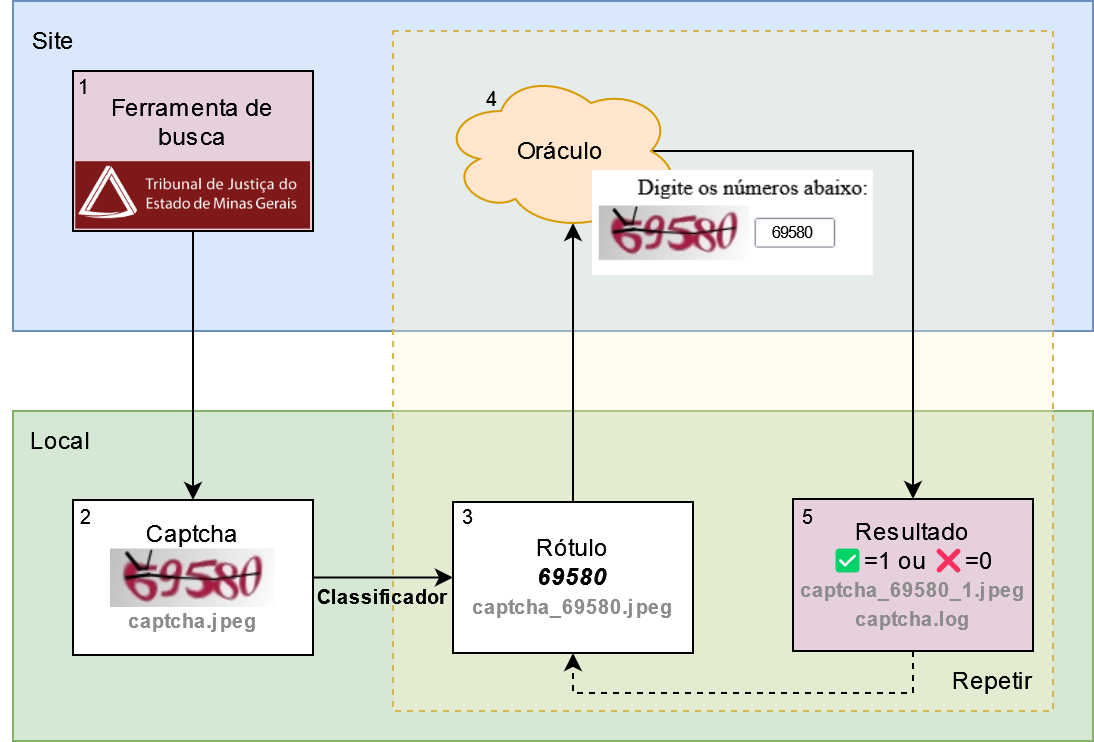
\includegraphics{./assets/img/esquema-oraculo.png}

}

\caption{\label{fig-esquema-oraculo}Esquema mostrando o funcionamento do
oráculo.}

\end{figure}

É possível generalizar naturalmente o oráculo para múltiplos chutes
mudando a definição da função que faz predições. Seja \(h\) uma função
que retorna um conjunto de \(k\) respostas possíveis,
\(k\in \mathbb N\), \(k\geq 1\), com \(\mathbf x_{n+1}\) e
\(\mathbf y_{n+1}\) iguais aos definidos definidos anteriormente. Então
o oráculo tem o funcionamento definido abaixo:

\[
\mathcal O(h(\mathbf x_{n+1})) = \left\{\begin{array}{ll}
    \{\mathbf y_{n+1}\}, & \text{ se } \mathbf y_{n+1} \in h(\mathbf x_{n+1})  \\
   \mathcal Y \setminus h(\mathbf x_{n+1}), & \text{ se } \mathbf y_{n+1} \notin h(\mathbf x_{n+1})
\end{array}\right..
\]

Nesse caso, o oráculo também retorna uma lista com a resposta
\(\mathbf y_{n+1}\). A única diferença é que, quando o Captcha aceita
múltiplos chutes, a lista retornada em caso de erro tem um comprimento
menor.

O oráculo tem um papel fundamental na solução proposta. O fato do
oráculo sempre retornar a resposta correta na lista de opções faz com
que ela necessariamente reduza o espaço de respostas a serem buscadas em
uma tentativa futura. Esse fato será explorado a partir de um método
iterativo para encontrar o valor real do rótulo.

\hypertarget{fatos-estilizados}{%
\subsubsection{Fatos estilizados}\label{fatos-estilizados}}

Historicamente, uma alternativa para resolver Captchas é separando o
problema em duas tarefas: segmentar e classificar. A tarefa de
segmentação consiste em receber uma imagem com várias letras e detectar
pontos de corte, separando-a em várias imagens de uma letra. Já a
classificação consiste em receber uma imagem com uma letra e identificar
o caractere correspondente. Nesse caso, a resposta é reduzida para
\(|\mathcal A|\) categorias, que cresce linearmente e, portanto,
tratável.

A tarefa de resolver Captchas também poderia ser vista como um problema
de reconhecimento óptico de caracteres (\emph{Optical Character
Recognition}, OCR). No entanto, as distorções encontradas em Captchas
são bem diferentes das distorções encontradas em textos escaneados, que
são o objeto de aplicação de ferramentas de OCR. Por esse motivo, as
ferramentas usuais de OCR apresentam resultados pouco satisfatórios em
vários Captchas.

As distorções encontradas em Captchas podem ser agrupadas em distorções
para dificultar a segmentação e distorções para dificultar a
classificação. Na parte de classificação, as principais formas de
dificultar o trabalho dos modelos são i) mudar as fontes (serifa ou sem
serifa ou negrito/itálico, por exemplo), ii) mudar letras minúsculas
para maiúsculas e iii) adicionar distorções nos caracteres. Já na parte
de segmentação, as principais formas são i) colar os caracteres e ii)
adicionar linhas ligando os dígitos. Essas técnicas são combinadas com a
adição de ruído e distorção nas imagens completas para compor a imagem
final.

\hypertarget{redes-neurais}{%
\subsection{Redes neurais}\label{redes-neurais}}

A abordagem discutida ao longo da tese utiliza redes neurais
convolucionais. Para explicar o funcionamento dessa técnica,
apresenta-se as definições para redes neurais e para a operação de
convolução no contexto de Captchas, construindo o modelo utilizado nas
simulações do modelo proposto.

A ideia abaixo é apresentar como funcionam as redes neurais no contexto
de Captchas. O modelo apresentado é o que foi utilizado nas simulações,
que é um modelo de redes neurais convolucionais simples, similar ao
LeNet, com três camadas convolucionais e duas camadas densas (LECUN et
al., 1998).

A técnica proposta pela tese pode utilizar diversas arquiteturas de
redes neurais. A escolha de uma arquitetura mais simples foi feita para
demonstrar a eficácia do procedimento de forma mais contundente. Outras
arquiteturas mais rebuscadas, como as apresentadas no referencial
teórico (GEORGE et al., 2017; YE et al., 2018) podem melhorar a
aplicação do modelo. A única restrição é que ela possa receber uma
função de perda modificada, como será mostrado a seguir.

É possível organizar a estrutura de uma rede neural em três componentes:
a \textbf{arquitetura da rede}, a \textbf{função de perda} e o
\textbf{otimizador}. Os componentes são detalhados nas próximas
subseções.

Como uma rede neural possui muitos componentes e subcomponentes, é usual
apresentar sua estrutura na forma de um diagrama. Redes neurais costumam
ser fáceis de representar através de grafos, que podem ser utilizados de
forma mais ou menos detalhada, dependento do interesse.

A Figura~\ref{fig-diagrama-modelo-cnn} mostra, de forma esquemática, os
componentes (retângulos tracejados) e subcomponentes (partes internas
dos componentes) do modelo utilizado.

\begin{figure}

{\centering 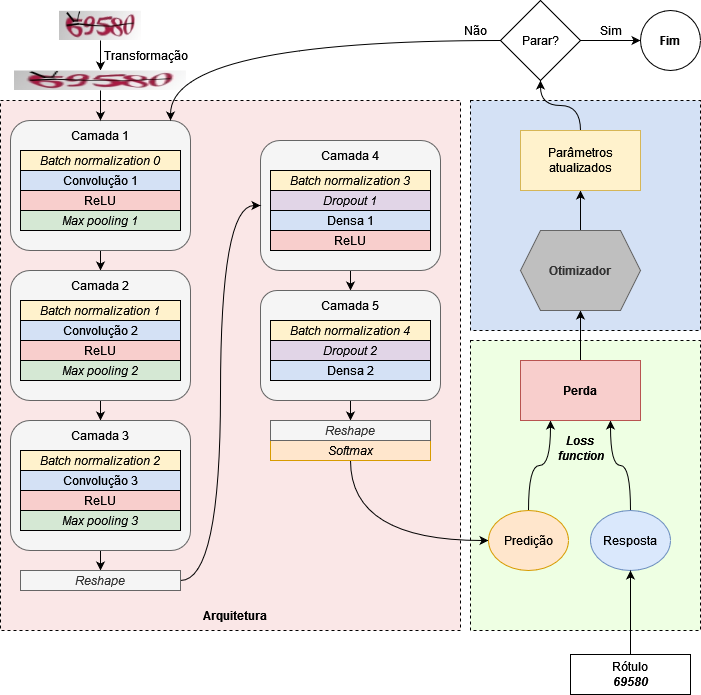
\includegraphics{./assets/img/diagrama-modelo-cnn.png}

}

\caption{\label{fig-diagrama-modelo-cnn}Diagrama representando o modelo
utilizado de forma genérica, com todos os componentes e subcomponentes
apresentados de forma esquemática. As partes de fora dos componentes são
entradas de dados ou decisões de parada do ajuste.}

\end{figure}

\hypertarget{sec-arquitetura-rede}{%
\subsubsection{Arquitetura da rede}\label{sec-arquitetura-rede}}

A arquitetura da rede é uma função que leva os dados de entrada na
estrutura de dados da variável resposta. A arquitetura tem papel similar
ao exercido pelo componente sistemático em um modelo linear generalizado
(NELDER; WEDDERBURN, 1972). Trata-se da parte mais complexa da rede
neural, carregando todos os parâmetros que serão otimizados.

A arquitetura da rede possui três componentes principais, separados em
dois itens cada:

\begin{itemize}
\tightlist
\item
  as camadas ocultas: camadas \textbf{convolucionais} e camadas
  \textbf{densas};
\item
  as técnicas de regularização: \textbf{normalização em lote}
  (\emph{batch normalization}), \textbf{\emph{dropout}} e junção de
  pixels (\emph{max pooling});
\item
  as funções de ativação: função de ativação linear retificada
  (\emph{rectified linear unit}, ReLU) e a função de normalização
  exponencial (\emph{softmax}).
\end{itemize}

Abaixo, apresenta-se as definições seguindo-se a ordem de aplicação das
operações na arquitetura da rede neural: camada convolucional, ReLU,
\emph{max pooling}, \emph{batch normalization}, \emph{dropout}, camada
densa e \emph{softmax}.

A \textbf{convolução} é uma operação linear que recebe como entrada uma
matriz e retorna outra matriz. Ela é diferente de uma operação usual de
multiplicação de matrizes vista no contexto de modelos lineares
generalizados, por envolver uma operação nos elementos na vizinhança de
cada pixel.

Uma forma organizada de fazer essa soma ponderada é criando uma matriz
de pesos. Com ela, não é necessário procurar os pontos da vizinhança.
Para cada ponto \((i,j)\), obtem-se a matriz de vizinhança,
multiplica-se pontualmente pela matriz de pesos e soma-se os valores
resultantes. A matriz de pesos é chamada de núcleo, ou \emph{kernel}.

Considere

\[
K = \left[\begin{array}{rrr}-1&-1&-1\\0&0&0\\1&1&1\end{array}\right]
\]

e a imagem da Figura~\ref{fig-tjmg-exemplo-conv}. Como visto
anteriormente, trata-de de uma matriz de dimensão
\(40\times110\times3\).

\begin{figure}

{\centering \includegraphics[width=1.14583in,height=\textheight]{./assets/img/tjmg16283c1e6d06.jpeg}

}

\caption{\label{fig-tjmg-exemplo-conv}Imagem de Captcha utilizado em
exemplos anteriores.}

\end{figure}

Tome por exemplo a primeira dimensão do pixel \((i,j,k) = (12,16,1)\). A
vizinhança 3x3 em torno desse ponto é dada por

\[
P_{i,j,k} = \left[\begin{array}{rrr}
0.094 & 0.412 & 0.686 \\ 
0.051 & 0.063 & 0.529 \\ 
0.071 & 0.000 & 0.086 
\end{array}\right]
\]

A operação de convolução é feita da seguinte forma:

\[
\begin{aligned}
(P_{12,16,1} *K )_{12,16,1}
&= k_{1,1}p_{11,15,1} + k_{1,2}p_{11,16,1} + k_{1,3}p_{11,17,1} + \\
&+ k_{2,1}p_{12,15,1} + k_{2,2}p_{12,16,1} + k_{2,3}p_{12,17,1} + \\
&+ k_{3,1}p_{13,15,1} + k_{3,2}p_{13,16,1} + k_{3,3}p_{13,17,1}
\end{aligned}
\]

Esse é o valor a ser colocado no ponto \((i,j,k)\). Isso funciona em
todos os pontos que não estão na borda da imagem.

Existem duas formas de trabalhar com as bordas da imagem. A primeira é
preenchendo as bordas com zeros, de forma a considerar apenas os pontos
da imagem. A segunda é descartar os pontos da borda e retornar uma
imagem menor, contendo somente os pixels em que foi possível aplicar
todo o \emph{kernel}.

No caso do exemplo, o resultado da convolução fica como na
Figura~\ref{fig-tjmg-exemplo-conv-horizontal}. A matriz não foi
escolhida por acaso: ela serve para destacar padrões horizontais da
imagem. Como a primeira linha é formada por \(-1\) e a última é formada
por \(1\), a matriz fica com valor alto se a parte de cima do pixel for
preta e a parte de baixo for branca
(\(\text{grande} * 1 + \text{pequeno} * (-1)\)). A parte destacada da
imagem acabou sendo a parte de baixo dos números e, principalmente, a
linha que une os números.

\begin{figure}

{\centering \includegraphics[width=1.14583in,height=\textheight]{./assets/img/tjmg_conv_horizontal.jpeg}

}

\caption{\label{fig-tjmg-exemplo-conv-horizontal}Aplicação de uma
convolução com kernel horizontal.}

\end{figure}

Aplicando o kernel vertical abaixo

\[
K = \left[\begin{array}{rrr}-1&0&1\\-1&0&1\\-1&0&1\end{array}\right],
\]

as partes destacadas são as laterais dos números, conforme
Figura~\ref{fig-tjmg-exemplo-conv-vertical}.

\begin{figure}

{\centering \includegraphics[width=1.14583in,height=\textheight]{./assets/img/tjmg_conv_vertical.jpeg}

}

\caption{\label{fig-tjmg-exemplo-conv-vertical}Aplicação de uma
convolução com kernel vertical.}

\end{figure}

O resultado da convolução pode ter números negativos ou maiores que um.
Para que seja possível visualizar, as imagens mostradas acima foram
normalizadas.

Uma característica das imagens mostradas acima é que elas ficaram
escuras, ou seja, com muitos valores próximos de zero. Uma técnica para
modificar a imagem é adicionar uma constante numérica ao resultado da
convolução. Esse é o chamado \textbf{viés} (\emph{bias}) da convolução.

A Figura~\ref{fig-tjmg-exemplo-conv-vertical-bias} mostra o efeito de
adicionar um viés de \texttt{0.6} após aplicação da convolução com
kernel vertical. É possível idenificar claramente a diferença entre os
números (mais suaves) e as curvas usadas para conectar os números (mais
proeminetes).

\begin{figure}

{\centering \includegraphics[width=1.14583in,height=\textheight]{./assets/img/tjmg_conv_vertical_bias.jpeg}

}

\caption{\label{fig-tjmg-exemplo-conv-vertical-bias}Aplicação de uma
convolução com kernel vertical e viés.}

\end{figure}

Uma \textbf{camada convolucional} envolve a aplicação de convoluções com
\(d\) \emph{kernels} em uma matriz, além da adição do \emph{bias}. O
resultado da aplicação de uma camada convolucional com preenchimento das
bordas é uma matriz com as mesmas dimensões \(N\) e \(M\) da matriz de
entrada, mas com \(d\) entradas na dimensão das cores. Como o valor de
\(d\) pode ser diferente de 1 ou 3, não faz mais sentido tratar essa
dimensão como cores, por isso essa dimensão é chamada de \textbf{canais}
da imagem resultante.

É importante notar que, nos exemplos apresentados anteriormente, a
convolução foi aplicada a apenas um dos canais da imagem: o primeiro.
Quando a imagem de entrada possui vários canais, camada convolucional
aplica cada \emph{kernel} em cada canal da imagem e, depois, faz a soma
dos valores resultantes.

A Figura~\ref{fig-tjmg-exemplo-camada-conv} mostra um exemplo de
aplicação de camada convolucional para a imagem utilizada nos exemplos
anteriores. Os \emph{kernels} foram escolhidos com base em um modelo que
já foi ajustado para o Captcha. Note que os canais capturam a informação
dos números e dos ruídos, focando em detalhes diferentes.

\begin{figure}

{\centering \includegraphics{./assets/img/tjmg_conv1_modelo.jpeg}

}

\caption{\label{fig-tjmg-exemplo-camada-conv}Resultado da aplicação da
primeira convolução à imagem.}

\end{figure}

Antes da aplicação da camada convolucional, a operação de
\textbf{\emph{batch normalization}} foi aplicada. Essa operação
normaliza os números da matriz de entrada antes da aplicação da
convolução, retirando a média e dividindo pelo desvio padrão.

\[
x_z = \left(\frac{x-\bar x}{\sqrt{\sigma^2_x + \epsilon}}\right) \gamma + \beta
\]

O valor \(\epsilon\), geralmente um valor pequeno, é adicionado para
evitar problemas numéricos quando a variância é muito baixa. Os
parâmetros \(\gamma\) e \(\beta\) podem ser adicionados no passo da
normalização, fazendo parte do fluxo de aprendizagem do modelo. Apesar
de não ser uma teoria fechada, alguns resultados indicam que o uso de
\emph{batch normalization} reduz o tempo de aprendizado dos modelos
(IOFFE; SZEGEDY, 2015). O passo foi adicionado nos modelos por
apresentar bons resulados nas simulações.

Após a aplicação da convolução, também é aplicada a função não linear
\textbf{ReLU}. A transformação ReLU é a mais simples das funções da
ativação, sendo igual à função identidade quando a entrada é positiva e
zero caso contrário:

\[
\text{ReLU}(x) = xI_{(x>0)}.
\]

A função ReLU serve para tornar a arquitetura do modelo uma operação não
linear. Qualquer operação não linear poderia ser utilizada, mas a mais
simples e mais popular é a ReLU.

Em seguida, aplica-se uma operação para reduzir a dimensão da imagem,
chamada \textbf{\emph{max pooling}}. Trata-se de uma operação que recebe
a imagem e um \emph{kernel}, retornando, para cada janela, o maior valor
dos pixels. Usualmente, a técnica também utiliza \emph{strides} fazendo
com que cada pixel seja avaliado apenas uma vez. Por exemplo, para uma
matriz com dimensões \(M_{10\times10}\) e \emph{kernel} com dimensões
\(2\times2\), o resultado é uma matriz \(M^p_{5\times5}\) onde cada
elemento é o valor máximo da janela correspondente ao pixel.

A operação \emph{max pooling} é muito comum no contexto de redes neurais
convolucionais. Sua aplicação é importante para que os \emph{kernels}
sejam aplicados em diferentes níveis da imagem de entrada.

A aplicação das camadas convolucionais é repetida três vezes. Ou seja,
as seguintes operações são aplicadas a partir da imagem original:

\begin{enumerate}
\def\labelenumi{\arabic{enumi}.}
\tightlist
\item
  \emph{batch normalization}: 6 parâmetros
\item
  camada convolucional: 896 parâmetros
\item
  ReLU
\item
  \emph{max pooling}
\item
  \emph{batch normalization}: 64 parâmetros
\item
  camada convolucional: 18.496 parâmetros
\item
  ReLU
\item
  \emph{max pooling}
\item
  \emph{batch normalization}: 128 parâmetros
\item
  camada convolucional: 36.928 parâmetros
\item
  ReLU
\item
  \emph{max pooling}
\item
  \emph{batch normalization}: 128 parâmetros
\end{enumerate}

A dimensão da imagem de entrada, bem como quantidade de canais gerados
por cada camada convolucional foram fixadas. Tais números podem ser
considerados como hiperparâmetros do modelo, mas foram fixados para
facilitar as simulações, que já contam com diversos hiperparâmetros.

A imagem de entrada foi fixada na dimensão \(32\times192\). O valor foi
definido dessa forma porque um dos Captchas de referência, da Receita
Federal do Brasil (RFB), possui 6 letras e \(32*6=192\). Ou seja, é como
se a imagem fosse a colagem lado a lado de 6 imagens \(32\times32\).

A quantidade de canais gerados pelas camadas convolucionais foram
fixadas em 32, 64 e 64. A utilização de números crescentes de canais nas
camadas convolucionais é comum (LECUN et al., 1998), bem como a
utilização de números que são potências de 2 (LECUN; BENGIO; HINTON,
2015). Nesse sentido, um possível valor para a terceira camada era de
128 canais, mas optou-se por 64 canais para que a quantidade de
parâmetros não ficasse grande demais, já que isso exigiria mais tempo de
computação e computadores mais poderosos.

O total de parâmetros que podem ser otimizados até o final das camadas
convolucionais é 56.646. Esse número pode parecer grande no contexto de
modelos estatísticos tradicionais como uma regressão linear, que teria,
considerando cada pixel como uma covariável, 4.401 parâmetros
(\(40\times110\) e o intercepto). No entanto, é uma quantidade
relativamente pequena no contexto de redes neurais. Redes neurais
recentes aplicadas a imagens, como o DALL-E 2 possui 3,5 bilhões de
parâmetros (RAMESH et al., 2022).

Em seguida, o resultado é transformado para um formato retangular,
similar ao que se encontra em modelos de regressão. Aqui, as dimensões
da imagem não são mais importantes e os pixels de cada canal são
tratados como variáveis preditoras. Esse passo pode ser interpretado da
seguinte forma: as camadas convolucionais funcionam como um
pré-processamento aplicado às imagens, como uma engenharia de variáveis
(KUHN; JOHNSON, 2019) otimizada, já que os parâmetros são ajustados no
modelo.

Uma vez obtidas as variáveis preditoras com o pré-processamento, é a
hora de aplicar as camadas densas. Tais camadas são as mais comuns no
contexto de redes neurais. Nesse caso, a operação linear aplicada é uma
multiplicação de matrizes, similar ao que é feito em um modelo linear
generalizado. Na verdade, o componente sistemático de um modelo linear
generalizado é equivalente a uma camada densa com a aplicação de viés,
com a função de ativação da fazendo o papel da função de ligação.

Assim como existem os canais das camadas convolucionais, existem os
filtros das camadas densas. A quantidade de filtros define a dimensão do
vetor de saída. O número de parâmetros da camada densa é igual ao número
de itens no vetor de entrada multiplicado pelo número de filtros, somado
à quantidade de filtros novamente, por conta do \emph{bias}. No caso do
exemplo, a saída das camadas convolucionais tem dimensão
\(2\times22\times64\) , ou seja, 64 canais de imagens \(2\times 22\).
Com a transformação em vetor, a quantidade de colunas da base passa a
ser a multiplicação das dimensões, ou 2.816. No modelo ajustado que foi
utilizado como exemplo, aplicou-se 200 filtros na camada densa,
totalizando 563.400 parâmetros. Nas simulações, a quantidade de filtros
foi variada para produzir modelos com menor ou maior capacidade.

É no contexto da grande quantidade de parâmetros que entra o conceito do
\emph{dropout} (BALDI; SADOWSKI, 2013). Trata-se de uma regra de
regularização muito simples de implementar, mas que possui grande
impacto no ajuste dos modelos. A técnica consiste em selecionar uma
amostra dos parâmetros em uma das camadas e apagá-los, forçando que os
valores sejam fixados em zero. Na prática, essa técnica obriga o modelo
a ser ajustado de forma que amostras aleatórias dos parâmetros sejam
boas para predizer a variável resposta. Quando o modelo ajustado é usado
para inferências, o \emph{dropout} é desativado e o modelo pode utilizar
todos os parâmetros, obtendo-se, na prática, uma média ponderada das
predições de cada sub-modelo. Dessa forma, o dropout tem um efeito
similar à aplicação da técnica de \emph{bagging} (GALAR et al., 2011),
muito utilizada na área de árvores de decisão.

O \emph{dropout} é aplicado após a finalização das camadas
convolucionais. Em seguida, vem a primeira camada densa, um ReLU e um
\emph{batch normalization}. Depois, é aplicada mais um \emph{dropout} e
mais uma camada densa. Com isso, a aplicação de operações é finalizada.
O total de parâmetros na configuração do modelo apresentado foi de
630.496. Os modelos mais simples utilizados nas simulações, com 100
filtros na camada densa, têm 343.696. Os mais complexos, com 300 filtros
na camada densa, têm 917.396 parâmetros.

Para finalizar a arquitetura do modelo, as quantidades resultantes devem
ser ajustadas ao formato da variável resposta. O número de filtros da
segunda camada densa precisa ser escolhido cuidadosamente, pois deve ser
igual à multiplicação das dimensões da variável resposta. No caso do
TJMG, os rótulos têm comprimento igual a 5 e vocabulário de comprimento
10 (algarismos arábicos), organizados em uma matriz \(5\times10\), com
50 entradas. Por isso, a quantidade de filtros da última camada densa
também é 50, e o vetor de saída é formatado para uma matriz de dimensão
\(5\times10\).

No final, o resultado precisa ser normalizado para que fique no mesmo
escopo de variação da resposta. A resposta possui apenas zeros e uns,
sendo que cada linha da matriz tem somente um número ``1'',
correspondendo ao índice do rótulo no alfabeto e, nas outras entradas, o
valor zero. A saída do modelo deve, portanto, apresentar números entre
zero e um que somam 1 em cada linha.

Isso é feito através da função \emph{softmax}, aplicada a cada linha da
matriz de saída. A função softmax é uma normalização que utiliza a
função exponencial no denominador, forçando que a soma dos valores do
vetor seja um.

\[
\text{soft}\max(y_i) = \frac{e^{y_i}}{\sum_{j=1}^{|\mathcal A|} e^{y_j}}
\]

No exemplo, a saída do modelo é a matriz abaixo:

\[
\hat{\mathbf z} = \left[\begin{array}{rrrrrrrrrr}
  -17.5 & -13.5 & -15.4 & -6.6 & -9.9 & 9.9 & -11.4 & -10.9 & -11.8 & -9.3 \\ 
  -10.9 & -15.6 & 8.3 & -6.5 & -11.0 & -10.3 & -10.0 & -5.8 & -11.4 & -15.1 \\ 
  -10.5 & -13.6 & -9.6 & -11.4 & 11.2 & -14.3 & -9.9 & -11.3 & -9.9 & -10.0 \\ 
  -18.1 & -9.6 & -10.9 & 5.3 & -10.1 & -6.6 & -15.5 & -13.3 & -6.8 & -10.8 \\ 
  -11.3 & -8.7 & 6.4 & -7.0 & -6.1 & -9.2 & -18.9 & -10.3 & -16.1 & -9.6 \\ 
\end{array}\right].
\]

Note que a matriz apresenta valores negativos e positivos. Na primeira
linha, por exemplo, o valor positivo está na sexta coluna,
correspondendo ao algarismo ``5''. De fato, esse é o valor do primeiro
elemento do rótulo para esta imagem. Após a aplicação do \emph{softmax},
a matriz de predições obtida é a matriz abaixo. O modelo de exemplo
aparenta ter confiança nas respostas, já que dá probabilidades bem altas
para alguns valores e quase zero para outros valores.

\[
\hat{\mathbf Y}\times 1000 = \left[\begin{array}{rrrrrrrrrr}
  0.00 & 0.00 & 0.00 & 0.00 & 0.00 & 1000.0 & 0.00 & 0.00 & 0.00 & 0.00 \\ 
  0.00 & 0.00 & 1000.0 & 0.00 & 0.00 & 0.00 & 0.00 & 0.00 & 0.00 & 0.00 \\ 
  0.00 & 0.00 & 0.00 & 0.00 & 1000.0 & 0.00 & 0.00 & 0.00 & 0.00 & 0.00 \\ 
  0.00 & 0.00 & 0.00 & 999.99 & 0.00 & 0.01 & 0.00 & 0.00 & 0.00 & 0.00 \\ 
  0.00 & 0.00 & 999.99 & 0.00 & 0.00 & 0.00 & 0.00 & 0.01 & 0.00 & 0.00 \\
\end{array}\right].
\]

Vale notar que, dependendo da implementação, nem sempre é necessário
aplicar a função \emph{softmax}. Em alguns pacotes computacionais como o
\texttt{torch}\footnote{Mais sobre o (py)torch:
  \url{https://pytorch.org}. Último acesso em 22 de novembro de 2022.},
utilizado nesta tese, a normalização pode ser feita diretamente na
função de perda, que aproveita a expressão completa para realizar
algumas simplificações matemáticas e, com isso, melhorar a precisão das
computações. O uso da função de perda ficará claro na próxima subseção.

\hypertarget{sec-funcao-perda-original}{%
\subsubsection{Perda}\label{sec-funcao-perda-original}}

A função de perda utilizada em um problema de classificação deve levar
em conta as probabilidades (ou log-probabilidades) associadas aos
rótulos. A perda deve ser pequena se a probabilidade associada ao rótulo
correto for alta e a perda deve ser grande se a probabilidade associada
ao rótulo correto for baixa.

Uma função de perda natural e popular nesse sentido é a de entropia
cruzada, ou \emph{cross-entropy}. Trata-se de uma perda com a formulação

\begin{equation}\protect\hypertarget{eq-perda-crossentropy}{}{
\mathcal L(g(x), y) = -\sum_{i=1}^c I(y=i)\log(g_i(x)),
}\label{eq-perda-crossentropy}\end{equation}

em que \(g_i(x)\) é a probabilidade dada ao rótulo \(i\) pela função
\(g\). Se o rótulo \(i\) é diferente do rótulo correto \(y\), a função
de perda vale zero por conta da função indicadora. Quando \(i=y\), a
perda é igual ao oposto do logaritmo da probabilidade associada ao
rótulo \(i\). Quanto menor a probabilidade, maior o valor da perda.

Ao trabalhar com o oráculo, a entropia cruzada passa a não fazer sentido
nos casos em que o modelo inicial erra. Por isso, a função de perda terá
de ser adaptada no método WAWL.

\hypertarget{sec-otimizador}{%
\subsubsection{Otimizador}\label{sec-otimizador}}

O otimizador utilizado para os modelos ajustados na tese foi o ADAM
(KINGMA; BA, 2017). A sigla significa \emph{Adaptive Moment Estimator} e
funciona como uma extensão da descida de gradiente estocástica (LECUN et
al., 2012), atualizando os parâmetros da seguinte forma:

\[
\begin{array}{cl}
m_{\theta}^{(t+1)} &\leftarrow \beta_1m_{\theta}^{(t)} + (1-\beta_1)\nabla_\theta L^{(t)} \\
v_{\theta}^{(t+1)} &\leftarrow \beta_2v_{\theta}^{(t)} + (1-\beta_2)(\nabla_\theta L^{(t)})^2 \\
\hat{m}_{\theta} &= \frac{m_\theta^{(t+1)}}{1-\beta_1^t} \\
\hat{v}_{\theta} &= \frac{v_\theta^{(t+1)}}{1-\beta_2^t} \\
\theta^{(t+1)} &\leftarrow \theta^{(t)} - \eta \frac{\hat{m}_{\theta}}{\sqrt{\hat{v}_{\theta}} + \epsilon},
\end{array}
\]

onde \(m\) e \(v\) são médias moveis para atualização dos parâmetros,
ponderando a perda e a perda ao quadrado com o passo anterior usando
pesos \(\beta_1\) e \(\beta_2\), respectivamente. Nessa notação \(\eta\)
é a taxa de aprendizado, um hiperparâmetro a ser ajustado. Por último, o
valor de \(\epsilon\) é uma constante, usualmente pequena, para evitar
divisão por zero.

\hypertarget{aprendizado-estatuxedstico}{%
\subsection{Aprendizado estatístico}\label{aprendizado-estatuxedstico}}

Apresentados o objeto de estudo, as redes neurais utilizadas e a
proposta da pesquisa, passa-se a discutir o significado disso tudo no
contexto de aprendizado estatístico. Essa parte foi escrita para
proporcionar a base teórica e a notação para apresentar as propriedades
do modelo WAWL.

O aprendizado fracamente supervisionado pode ser dividido em três tipos
principais. A supervisão com erros, a supervisão com rótulos incompletos
e a supervisão de grupos de observações. O caso do Captcha pode ser
entendido como uma sub-área do aprendizado fracamente supervisionado com
rótulos incompletos chamada aprendizado com dados parcialmente rotulados
(PLL), já que uma parte da base pode ser anotada sem erros e uma parte
da base é a resposta do oráculo indicando uma lista de rótulos possíveis
incluindo o correto.

A área de PLL não é nova (GRANDVALET, 2002) e aparece com outros nomes,
como aprendizado com rótulos ambíguos (HÜLLERMEIER; BERINGER, 2006) e
aprendizado de rótulos em superconjuntos (\emph{superset-label
learning)} (LIU; DIETTERICH, 2012). Um caso particular de PLL, aplicável
ao tema do Captcha são rótulos complementares (ISHIDA et al., 2017), que
considera os chutes errados na notação do problema.

As definições seguem uma terminologia adaptada a partir da leitura de
JIN; GHAHRAMANI (2002), COUR; SAPP; TASKAR (2011) e FENG et al. (2020a).
Sempre que possível, os casos são adaptados para o problema do Captcha
diretamente. Quando necessário, apresenta-se primeiro a definição
genérica e depois a formulação para o Captcha.

Em um problema de aprendizado supervisionado tradicional, tem-se um
conjunto de casos rotulados \(S=\{(\mathbf x_i,y_i), i=1,\dots, m\}\)
com uma distribuição \(p(\mathbf X,Y)\) desconhecida, onde
\(\mathbf X\in \mathcal X\) é uma imagem e \(Y\) é o rótulo, que possui
\(|\mathcal A|\) possíveis valores. O objetivo é obter um classificador
\(g\) que leva um valor de \(\mathbf x\) para o rótulo correto \(y\).

Para delimitar se o classificador está bom ou ruim, utiliza-se uma
função de perda. No caso do Captcha, como o interesse é simplesmente
acertar o rótulo inteiro (não importa se o classificador acerta só uma
parte do rótulo), utiliza-se uma função chamada 0-1:

\begin{equation}\protect\hypertarget{eq-perda}{}{
\mathcal L(g(\mathbf x),\mathbf y) = I (g(\mathbf x) \neq \mathbf y),
}\label{eq-perda}\end{equation}

em que \(I(\cdot)\) é uma função indicadora. Como a função de perda é
aplicada a apenas um par \((\mathbf x,y)\), define-se formalmente que o
objetivo do problema de aprendizado é minimizar o \emph{risco}, que é o
valor esperado da função de perda:

\begin{equation}\protect\hypertarget{eq-risco}{}{
\mathcal R(g) = \mathbb E_{p(\mathbf X,Y)}[\mathcal L(g(\mathbf X),Y)].
}\label{eq-risco}\end{equation}

A função de risco, no entanto, não é observada, já que depende da
distribuição desconhecida de \(p(\mathbf X,Y)\). Por isso utiliza-se um
estimador do risco, que pode ser calculado em bases usadas na validação
cruzada e na base de teste.

\[
\hat{\mathcal R}(g) = \sum_{i=1}^n \mathcal L(g(\mathbf x_i),y_i))
\]

Na base de teste, utilizada para estimar o risco, a função de perda 0-1
é apropriada. Na etapa de validação cruzada de um modelo de aprendizado
profundo, é útil considerar uma função de perda que seja contínua e
derivável, funcionando como uma versão suavizada da perda 0-1. A partir
de um vetor de parâmetros \(\boldsymbol \theta\) originados da
arquitetura do modelo, uma escolha de função de perda é a entropia
cruzada, como na Equação~\ref{eq-perda-crossentropy}. Os parâmetros são
estimados a partir de um otimizador, como o ADAM, apresentado na
Seção~\ref{sec-otimizador}.

As definições começam a precisar de ajustes quando \(y\) deixa de ser um
rótulo fixado. Como descrito na Seção~\ref{sec-oraculo}, a base de dados
observada contém tanto rótulos observados de forma exata quanto rótulos
apenas parcialmente informados. Nesse caso, os dados são gerados por uma
distribuição

\[
p(\mathbf X,\mathbf Y,\bar{\mathbf Y})=p(\mathbf X, \mathbf Y)p(\bar{\mathbf Y}|\mathbf X,\mathbf Y),
\]

em que \(\bar{\mathbf Y}\) é um conjunto de rótulos \emph{incorretos}.
Nesse caso observam-se, além das instâncias
\((\mathbf x_i,\mathbf y_i)\) quando o modelo inicial acerta, as
instâncias \((\mathbf x_j, \bar{\mathbf {y}}_j)\) quando o modelo
inicial erra. Supondo que \(\bar{\mathbf Y}\) é condicionalmente
independente de \({\mathbf Y}\) dado \({\mathbf X}\), temos que

\[
p(\mathbf X,\mathbf Y,\bar{\mathbf Y})=p(\mathbf X, \mathbf Y)p(\bar{\mathbf Y}|\mathbf Y).
\]

No caso dos Captchas, essa suposição é verificada. A probabilidade do
modelo inicial errar depende apenas do rótulo e não das distorções
realizadas pela imagem gerada a partir do rótulo. Além disso, a partir
do modelo inicial, é possível estimar os valores de
\(p(\bar{\mathbf Y}|\mathbf Y)\) a partir da base de teste utilizada
para medir a acurácia do modelo.

Nos casos em que \(|\hat{\mathbf Y}|=1\), as probabilidades
\(p(\bar{\mathbf Y}|\mathbf Y)\) podem ser organizadas em uma matriz de
transição \(\mathbf Q\), contendo as probabilidades de se obter um
rótulo incorreto para cada possível valor do rótulo. Isso acontece nos
Captchas em que não é possível realizar múltiplos chutes. Para resolver
problemas desse tipo, é possível realizar um ajuste na função de
predição que a torna a função de perda consistente e com taxa de
convergência conhecida (YU et al., 2018):

\[
f_{\text{adj}} (\mathbf X) = \mathbf Q ^{\top}f(\mathbf X)
\]

O tipo de problema apresentado acima é conhecido como \emph{biased
complementary label}, ou seja, rótulo complementar com viés. Também é
possível considerar um caso sem viés, ou seja, quando
\(p(\bar{\mathbf Y}|\mathbf Y) = \frac{1}{c-1}\) para todos os valores
de \(\mathbf Y\) e uma constante \(c\). Esse caso também foi resolvido
do ponto de vista teórico (ISHIDA et al., 2017). As conclusões são
parecidas, ou seja, é possível encontrar taxas de convergência para que
o problema com rótulos complementares se aproxime de um problema com
observações completas.

Quando os rótulos complementares não apresentam viés, existe ainda uma
extensão para rótulos complementares múltiplos (FENG et al., 2020b).
Neste caso, é possível derivar uma função de risco empírica que,
novamente, converge para a função de risco do problema completamente
supervisionado, além de apresentar taxas de convergência para essa
função de risco.

O caso do oráculo e dos Captchas é um problema com múltiplos rótulos
complementares e com viés. Até o momento, não existe uma solução geral
para este tipo de problema. No entanto, espera-se que as soluções para
problemas desse tipo tenham taxas de convergência mais estreitas do que
o caso de rótulos complementares, com ou sem viés, já que rótulos
complementares múltiplos trazem mais informação do que rótulos
complementares simples.

\hypertarget{sec-wawl}{%
\section{Método WAWL}\label{sec-wawl}}

O método WAWL (\emph{Web Automatic Weak Learning}) é a solução proposta
na pesquisa. Trata-se da técnica baixar dados da web para compor parte
da amostra que é utilizada no ajuste do modelo.

O método WAWL é inovador por dois motivos. Primeiro, porque o método faz
a ponte entre áreas que até o momento eram partes separadas do ciclo da
ciência de dados: a raspagem de dados e o aprendizado estatístico. Além
disso, o método é uma nova alternativa para resolver Captchas com pouca
ou nenhuma intervenção humana.

Existem duas formas principais de aplicar o método WAWL. A primeira
criando novas bases de treino a partir de um modelo inicial e
atualizando os modelos com os dados baixados. A segunda é baixando os
dados dentro do próprio ciclo de ajuste do modelo, acessando a web no
momento de construção de um \emph{minibatch}.

A arquitetura do modelo WAWL pode ser a mesma de um modelo ajustado com
uma base completamente anotada. O modelo pode, inclusive, aproveitar os
parâmetros já ajustados em uma eventual versão inicial do modelo para
acelerar o aprendizado. Nada impede, no entanto, que uma arquitetura
diferente seja utilizada, desde que a entrada seja uma imagem e a saída
seja uma matriz com as dimensões da variável resposta. O WAWL é
agnóstico à arquitetura do modelo.

A função de perda deve ser adaptada para considerar a informação
limitada fornecida pelo oráculo. Quando o rótulo fornecido pelo modelo
está correto, a informação é considerada normalmente, através da função
de perda da regressão multinomial multivariada. Já quando o rótulo
fornecido pelo modelo é incorreto, a função de perda é calculada com
base na probabilidade do rótulo estar incorreto:

\[
1 - p(\mathbf y|\boldsymbol \theta),
\]

Considerando o rótulo complementar \(\bar y\) e a função \(f\) dada pela
rede neural, a fórmula para descrever a função de perda é descrita da
seguinte forma:

\[
\mathcal L(\bar y, f(\mathbf x)) = -\log\left[1 - \sum_{y} {f_y}(\mathbf x) I(y=\bar y)\right]
\]

A função de perda proposta pode ser explicada de maneira intuitiva
através de um exemplo. Considere um problema com apenas \(c\) possíveis
valores para o rótulo (ou seja, uma resposta multinomial, sem ser
multivariada). Considere também que a rede neural retorna uma alta
probabilidade, por exemplo, \(0.99\), para o valor \(i\), que o oráculo
identificou como incorreta. Nesse caso, a função de perda é dada por

\[
\mathcal L(i,f(\mathbf x)) = -\log\left[1-{f_i}(\mathbf x)\right] = -\log\left[1-0.99 \right] = 4.61
\]

Como é possível ver no exemplo, quanto maior a probabilidade dada a um
rótulo identificado como incorreto pelo oráculo, mais a função de perda
penaliza essa predição. Dessa forma, a função de perda consegue
incorporar completamente a informação dada pelo oráculo.

Quando o Captcha aceita múltiplos chutes, a mesma conta é válida,
bastando subtrair as probabilidades de todos os rótulos incorretos:

\[
\mathcal L(\bar {\mathbf y}, f(\mathbf x)) = -\log\left[1 - \sum_{y} {f_y}(\mathbf x) I(y \in \bar {\mathbf y})\right]
\]

No final, o valor que é passado para a função de perda é a soma das
perdas para todas as observações do \emph{minibatch}. A soma considera
tanto as perdas calculadas com base nos rótulos corretos quanto as
perdas calculadas com base nos rótulos incorretos.

O otimizador que obtém novas estimativas dos parâmetros também não
precisa ser modificado. Basta aplicar a mesma técnica utilizada na
modelagem usual, como descida de gradiente estocástica ou métodos
adaptativos, como o ADAM.

Um detalhe importante sobre o método é sobre a implementação. Com a
utilização de ferramentas que fazem diferenciação automática como o
\emph{torch} e o \emph{TensorFlow}\footnote{Mais detalhes em
  \url{https://www.tensorflow.org}. Último acesso em 22 de novembro de
  2022.}, basta implementar a parte da arquitetura, a função de perda e
especificar o otimizador, já que o processo de atualização dos
parâmetros é feito automaticamente. No entanto, dependendo da
implementação, não é possível fazer a atualização dos parâmetros usando
o componente de computação gráfica, que potencialmente acelera o ajuste
dos modelos de forma significativa. Na implementação atual, a função de
perda apresentada não permite utilização desse componente, sendo uma
melhoria possível em futuros trabalhos.

O ajuste dos modelos, tanto para simulações quanto para construção dos
modelos finais, utilizou o pacote \texttt{\{torch\}} (FALBEL; LURASCHI,
2022), que é uma implementação do PyTorch para a linguagem de
programação R (R CORE TEAM, 2021). O pacote \texttt{\{luz\}} (FALBEL,
2022a) foi utilizado para organizar as funções de perda e
hiperparâmetros, enquanto o pacote \texttt{\{torchvision\}} (FALBEL,
2022b) foi utilizado para utilidades no tratamento de imagens.

\hypertarget{dados}{%
\section{Dados}\label{dados}}

Nesta seção, descreve-se em detalhes como foi a obtenção dos dados para
realizar a pesquisa. Como comentado anteriormente, a base foi construída
do zero para os fins do projeto, sendo uma parte significativa dos
esforços para chegar nos resultados.

No total, foram construídas bases de dados de dez Captchas que estavam
disponíveis publicamente no período de realização da pesquisa. Os
Captchas foram revisados pela última vez no dia 14/09/2022, para
verificar se ainda estavam ativos. Além disso, foram construídas duas
bases de dados de Captchas desenvolvidos internamente para fins de
teste.

Parte dos dados foram obtidos como um passo intermediário das
simulações. A presente seção descreve como os robôs de coleta foram
construídos, bem como a metodologia para obter rótulos via classificação
manual. Na subseção de dados da seção de simulação, é possível acessar
informações sobre os dados baixados para realizar as simulações.

\hypertarget{escolha-dos-captchas-analisados}{%
\subsection{Escolha dos Captchas
analisados}\label{escolha-dos-captchas-analisados}}

Para selecionar os Captchas, foram adotados alguns critérios objetivos.
Os critérios foram:

\begin{enumerate}
\def\labelenumi{\arabic{enumi}.}
\tightlist
\item
  O site acessado é de um serviço público (governo federal, tribunal,
  etc).
\item
  O Captcha contém letras (A a Z) e números (0 a 9) em uma imagem com
  extensão \texttt{jpeg} ou \texttt{png}.
\item
  O comprimento do Captcha é fixo, ou seja, dois Captchas da mesma
  origem devem ter sempre o mesmo comprimento.
\end{enumerate}

A primeira restrição para escolha dos Captchas é de ordem
principiológica. Um serviço público não deveria restringir o acesso aos
dados para robôs. Como já discutido anteriormente, nesses casos, a
existência do Captcha não tem como finalidade dar maior segurança ao
serviço prestado, mas sim limitar o acesso aos servidores por robôs.

As restrições 2 e 3 foram escolhidas com o objetivo de facilitar as
simulações para obtenção dos resultados. Em princípio, nada impede que
os modelos desenvolvidos trabalhem com outros tipos de rótulos, desde
que exista uma lista prévia de rótulos. Além disso, é possível realizar
adaptações no pré-processamento base de dados para lidar com diferentes
comprimentos de Captchas.

A Tabela~\ref{tbl-lista-captcha} mostra os Captchas trabalhados. Dos 10
exemplos trabalhados, 6 têm origem em tribunais, que são conhecidos por
não disponibilizarem os dados de forma aberta.

\hypertarget{tbl-lista-captcha}{}
\begin{table}[H]

\providecommand{\docline}[3]{\noalign{\global\setlength{\arrayrulewidth}{#1}}\arrayrulecolor[HTML]{#2}\cline{#3}}

\setlength{\tabcolsep}{0pt}

\renewcommand*{\arraystretch}{1.5}

\begin{longtable}[c]{|p{0.75in}|p{1.50in}|p{3.00in}}

\caption{\label{tbl-lista-captcha}Lista de captchas analisados. } \\ 


\hhline{>{\arrayrulecolor[HTML]{000000}\global\arrayrulewidth=1pt}->{\arrayrulecolor[HTML]{000000}\global\arrayrulewidth=1pt}->{\arrayrulecolor[HTML]{000000}\global\arrayrulewidth=1pt}-}

\multicolumn{1}{!{\color[HTML]{000000}\vrule width 0pt}>{\centering}p{\dimexpr 0.75in+0\tabcolsep+0\arrayrulewidth}}{\textcolor[HTML]{000000}{\fontsize{11}{22}\selectfont{Captcha}}} & \multicolumn{1}{!{\color[HTML]{000000}\vrule width 0pt}>{\centering}p{\dimexpr 1.5in+0\tabcolsep+0\arrayrulewidth}}{\textcolor[HTML]{000000}{\fontsize{11}{22}\selectfont{Exemplo}}} & \multicolumn{1}{!{\color[HTML]{000000}\vrule width 0pt}>{\centering}p{\dimexpr 3in+0\tabcolsep+0\arrayrulewidth}!{\color[HTML]{000000}\vrule width 0pt}}{\textcolor[HTML]{000000}{\fontsize{11}{22}\selectfont{Descrição}}} \\

\hhline{>{\arrayrulecolor[HTML]{000000}\global\arrayrulewidth=1pt}->{\arrayrulecolor[HTML]{000000}\global\arrayrulewidth=1pt}->{\arrayrulecolor[HTML]{000000}\global\arrayrulewidth=1pt}-}\endhead



\multicolumn{1}{!{\color[HTML]{000000}\vrule width 0pt}>{\centering}p{\dimexpr 0.75in+0\tabcolsep+0\arrayrulewidth}}{\textcolor[HTML]{000000}{\fontsize{11}{22}\selectfont{\href{https://pje.trf5.jus.br/pje/ConsultaPublica/listView.seam}{trf5}}}} & \multicolumn{1}{!{\color[HTML]{000000}\vrule width 0pt}>{\centering}p{\dimexpr 1.5in+0\tabcolsep+0\arrayrulewidth}}{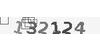
\includegraphics[width=0.9in, height=0.45in]{metodologia_files/figure-pdf/tbl-lista-captcha-1.png}} & \multicolumn{1}{!{\color[HTML]{000000}\vrule width 0pt}>{\centering}p{\dimexpr 3in+0\tabcolsep+0\arrayrulewidth}!{\color[HTML]{000000}\vrule width 0pt}}{\textcolor[HTML]{000000}{\fontsize{11}{22}\selectfont{Tribunal\ Regional\ Federal\ 5}}} \\





\multicolumn{1}{!{\color[HTML]{000000}\vrule width 0pt}>{\centering}p{\dimexpr 0.75in+0\tabcolsep+0\arrayrulewidth}}{\textcolor[HTML]{000000}{\fontsize{11}{22}\selectfont{\href{https://www4.tjmg.jus.br/juridico/sf/proc\_resultado.jsp?comrCodigo=24\&numero=1\&listaProcessos=50718889720218130024\&btn\_pesquisar=Pesquisar}{tjmg}}}} & \multicolumn{1}{!{\color[HTML]{000000}\vrule width 0pt}>{\centering}p{\dimexpr 1.5in+0\tabcolsep+0\arrayrulewidth}}{
\includegraphics[width=0.9in, height=0.45in]{metodologia_files/figure-pdf/tbl-lista-captcha-2.png}} & \multicolumn{1}{!{\color[HTML]{000000}\vrule width 0pt}>{\centering}p{\dimexpr 3in+0\tabcolsep+0\arrayrulewidth}!{\color[HTML]{000000}\vrule width 0pt}}{\textcolor[HTML]{000000}{\fontsize{11}{22}\selectfont{Tribunal\ de\ Justiça\ de\ Minas\ Gerais}}} \\





\multicolumn{1}{!{\color[HTML]{000000}\vrule width 0pt}>{\centering}p{\dimexpr 0.75in+0\tabcolsep+0\arrayrulewidth}}{\textcolor[HTML]{000000}{\fontsize{11}{22}\selectfont{\href{https://pje-consulta.trt3.jus.br/pje-consulta-api/api/processos/2104879}{trt}}}} & \multicolumn{1}{!{\color[HTML]{000000}\vrule width 0pt}>{\centering}p{\dimexpr 1.5in+0\tabcolsep+0\arrayrulewidth}}{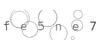
\includegraphics[width=0.9in, height=0.45in]{metodologia_files/figure-pdf/tbl-lista-captcha-3.png}} & \multicolumn{1}{!{\color[HTML]{000000}\vrule width 0pt}>{\centering}p{\dimexpr 3in+0\tabcolsep+0\arrayrulewidth}!{\color[HTML]{000000}\vrule width 0pt}}{\textcolor[HTML]{000000}{\fontsize{11}{22}\selectfont{Tribunal\ Regional\ do\ Trabalho\ 3}}} \\





\multicolumn{1}{!{\color[HTML]{000000}\vrule width 0pt}>{\centering}p{\dimexpr 0.75in+0\tabcolsep+0\arrayrulewidth}}{\textcolor[HTML]{000000}{\fontsize{11}{22}\selectfont{\href{http://esaj.tjba.jus.br/cpopg/open.do}{esaj}}}} & \multicolumn{1}{!{\color[HTML]{000000}\vrule width 0pt}>{\centering}p{\dimexpr 1.5in+0\tabcolsep+0\arrayrulewidth}}{
\includegraphics[width=0.9in, height=0.45in]{metodologia_files/figure-pdf/tbl-lista-captcha-4.png}} & \multicolumn{1}{!{\color[HTML]{000000}\vrule width 0pt}>{\centering}p{\dimexpr 3in+0\tabcolsep+0\arrayrulewidth}!{\color[HTML]{000000}\vrule width 0pt}}{\textcolor[HTML]{000000}{\fontsize{11}{22}\selectfont{Tribunal\ de\ Justiça\ da\ Bahia}}} \\





\multicolumn{1}{!{\color[HTML]{000000}\vrule width 0pt}>{\centering}p{\dimexpr 0.75in+0\tabcolsep+0\arrayrulewidth}}{\textcolor[HTML]{000000}{\fontsize{11}{22}\selectfont{\href{https://www.jucesponline.sp.gov.br/ResultadoBusca.aspx}{jucesp}}}} & \multicolumn{1}{!{\color[HTML]{000000}\vrule width 0pt}>{\centering}p{\dimexpr 1.5in+0\tabcolsep+0\arrayrulewidth}}{
\includegraphics[width=0.9in, height=0.45in]{metodologia_files/figure-pdf/tbl-lista-captcha-5.png}} & \multicolumn{1}{!{\color[HTML]{000000}\vrule width 0pt}>{\centering}p{\dimexpr 3in+0\tabcolsep+0\arrayrulewidth}!{\color[HTML]{000000}\vrule width 0pt}}{\textcolor[HTML]{000000}{\fontsize{11}{22}\selectfont{Junta\ Comercial\ de\ São\ Paulo}}} \\





\multicolumn{1}{!{\color[HTML]{000000}\vrule width 0pt}>{\centering}p{\dimexpr 0.75in+0\tabcolsep+0\arrayrulewidth}}{\textcolor[HTML]{000000}{\fontsize{11}{22}\selectfont{\href{https://srv01.tjpe.jus.br/consultaprocessualunificada/}{tjpe}}}} & \multicolumn{1}{!{\color[HTML]{000000}\vrule width 0pt}>{\centering}p{\dimexpr 1.5in+0\tabcolsep+0\arrayrulewidth}}{
\includegraphics[width=0.9in, height=0.45in]{metodologia_files/figure-pdf/tbl-lista-captcha-6.png}} & \multicolumn{1}{!{\color[HTML]{000000}\vrule width 0pt}>{\centering}p{\dimexpr 3in+0\tabcolsep+0\arrayrulewidth}!{\color[HTML]{000000}\vrule width 0pt}}{\textcolor[HTML]{000000}{\fontsize{11}{22}\selectfont{Tribunal\ de\ Justiça\ de\ Pernambuco}}} \\





\multicolumn{1}{!{\color[HTML]{000000}\vrule width 0pt}>{\centering}p{\dimexpr 0.75in+0\tabcolsep+0\arrayrulewidth}}{\textcolor[HTML]{000000}{\fontsize{11}{22}\selectfont{\href{https://www.tjrs.jus.br/site\_php/consulta/verificador.php}{tjrs}}}} & \multicolumn{1}{!{\color[HTML]{000000}\vrule width 0pt}>{\centering}p{\dimexpr 1.5in+0\tabcolsep+0\arrayrulewidth}}{
\includegraphics[width=0.9in, height=0.45in]{metodologia_files/figure-pdf/tbl-lista-captcha-7.png}} & \multicolumn{1}{!{\color[HTML]{000000}\vrule width 0pt}>{\centering}p{\dimexpr 3in+0\tabcolsep+0\arrayrulewidth}!{\color[HTML]{000000}\vrule width 0pt}}{\textcolor[HTML]{000000}{\fontsize{11}{22}\selectfont{Tribunal\ de\ Justiça\ do\ Rio\ Grande\ do\ Sul}}} \\





\multicolumn{1}{!{\color[HTML]{000000}\vrule width 0pt}>{\centering}p{\dimexpr 0.75in+0\tabcolsep+0\arrayrulewidth}}{\textcolor[HTML]{000000}{\fontsize{11}{22}\selectfont{\href{https://www.cadesp.fazenda.sp.gov.br/(S(vyfz1cfybbxj3sgpf4eqhxd3}{cadesp}}}} & \multicolumn{1}{!{\color[HTML]{000000}\vrule width 0pt}>{\centering}p{\dimexpr 1.5in+0\tabcolsep+0\arrayrulewidth}}{
\includegraphics[width=0.9in, height=0.45in]{metodologia_files/figure-pdf/tbl-lista-captcha-8.png}} & \multicolumn{1}{!{\color[HTML]{000000}\vrule width 0pt}>{\centering}p{\dimexpr 3in+0\tabcolsep+0\arrayrulewidth}!{\color[HTML]{000000}\vrule width 0pt}}{\textcolor[HTML]{000000}{\fontsize{11}{22}\selectfont{Centro\ de\ Apoio\ ao\ Desenvolvimento\ da\ Saúde\ Pública}}} \\





\multicolumn{1}{!{\color[HTML]{000000}\vrule width 0pt}>{\centering}p{\dimexpr 0.75in+0\tabcolsep+0\arrayrulewidth}}{\textcolor[HTML]{000000}{\fontsize{11}{22}\selectfont{\href{https://sei.economia.gov.br/sei/modulos/pesquisa/md\_pesq\_processo\_pesquisar.php?acao\_externa=protocolo\_pesquisar\&acao\_origem\_externa=protocolo\_pesquisar\&id\_orgao\_acesso\_externo=0}{sei}}}} & \multicolumn{1}{!{\color[HTML]{000000}\vrule width 0pt}>{\centering}p{\dimexpr 1.5in+0\tabcolsep+0\arrayrulewidth}}{
\includegraphics[width=0.9in, height=0.45in]{metodologia_files/figure-pdf/tbl-lista-captcha-9.png}} & \multicolumn{1}{!{\color[HTML]{000000}\vrule width 0pt}>{\centering}p{\dimexpr 3in+0\tabcolsep+0\arrayrulewidth}!{\color[HTML]{000000}\vrule width 0pt}}{\textcolor[HTML]{000000}{\fontsize{11}{22}\selectfont{Sistema\ Eletrônico\ de\ Informações\ -\ ME}}} \\





\multicolumn{1}{!{\color[HTML]{000000}\vrule width 0pt}>{\centering}p{\dimexpr 0.75in+0\tabcolsep+0\arrayrulewidth}}{\textcolor[HTML]{000000}{\fontsize{11}{22}\selectfont{\href{https://servicos.receita.fazenda.gov.br/servicos/cnpjreva/Cnpjreva\_Solicitacao\_CS.asp}{rfb}}}} & \multicolumn{1}{!{\color[HTML]{000000}\vrule width 0pt}>{\centering}p{\dimexpr 1.5in+0\tabcolsep+0\arrayrulewidth}}{
\includegraphics[width=0.9in, height=0.45in]{metodologia_files/figure-pdf/tbl-lista-captcha-10.png}} & \multicolumn{1}{!{\color[HTML]{000000}\vrule width 0pt}>{\centering}p{\dimexpr 3in+0\tabcolsep+0\arrayrulewidth}!{\color[HTML]{000000}\vrule width 0pt}}{\textcolor[HTML]{000000}{\fontsize{11}{22}\selectfont{Receita\ Federal}}} \\

\hhline{>{\arrayrulecolor[HTML]{000000}\global\arrayrulewidth=1pt}->{\arrayrulecolor[HTML]{000000}\global\arrayrulewidth=1pt}->{\arrayrulecolor[HTML]{000000}\global\arrayrulewidth=1pt}-}



\end{longtable}

\end{table}

Além dos Captchas de sites, também foram consideradas imagens geradas
artificialmente. O motivo de criar Captchas artificiais é a facilidade
de rodar modelos e simulações, já que nos casos reais é necessário ter
acesso à internet e também construir bases de dados de cada Captcha.

Foram gerados dois tipos de Captchas artificiais. O primeiro, chamado
\textbf{MNIST-Captcha}, é simplesmente uma adaptação da conhecida base
MNIST para ficar no formato de um Captcha. A partir da escolha do
comprimento e dos caracteres que fazem parte da imagem, o gerador
simplesmente faz uma amostra aleatória da base do MNIST e compõe as
imagens horizontalmente.

A Figura~\ref{fig-captcha-mnist} mostra um exemplo do Captcha gerado a
partir da base MNIST. No exemplo, o comprimento escolhido para o Captcha
foi de 4 valores.

\begin{figure}

{\centering \includegraphics[width=1.5625in,height=\textheight]{./assets/img/mnist128c49c36e13_6297.png}

}

\caption{\label{fig-captcha-mnist}Exemplo de MNIST-Captcha}

\end{figure}

O problema do MNIST-Captcha é que a base de dados original é finita.
Apesar de possuir por volta de 60 mil observações e de um Captcha
crescer em ordem exponencial, o MNIST-Captcha pode gerar Captchas
repetidos. Além disso, é necessário tomar cuidado com as bases de treino
e teste, já que os elementos de teste não poderiam fazer parte de
nenhuma observação de treino.

Pelos motivos supracitados, também foi criado um Captcha gerado
inteiramente por programação, chamado \textbf{R-Captcha}. O Captcha é
gerado utilizando a ferramenta ImageMagick, com a possibilidade de
customizar diversos parâmetros, como

\begin{itemize}
\tightlist
\item
  Quais caracteres usar na imagem
\item
  O comprimento do Captcha
\item
  Dimensões da imagem
\item
  Probabilidade de rotação da imagem
\item
  Probabilidade de adicionar um risco entre as letras
\item
  Probabilidade de adicionar uma borda nas letras
\item
  Probabilidade de adicionar uma caixa (retângulo) em torno das letras
\item
  Probabilidade de adicionar um ruído branco no fundo da imagem
\item
  Probabilidade de adicionar efeitos de tinta óleo e implosão
\end{itemize}

A Figura~\ref{fig-captcha-r} mostra um exemplo de R-Captcha. O exemplo
apresenta uma linha ligando as letras, comprimento 4, dígitos maiúsculos
e minúsculos e distorções.

\begin{figure}

{\centering \includegraphics[width=1.5625in,height=\textheight]{./assets/img/captcha128c4a9c32e4_boy4.png}

}

\caption{\label{fig-captcha-r}Exemplo de MNIST-Captcha}

\end{figure}

Por ser uma versão mais flexível e completa, optou-se por trabalhar
principalmente com o R-Captcha nas simulações. O MNIST-Captcha foi
implementado mas não foi utilizado nas simulações.

\hypertarget{construuxe7uxe3o-dos-dados}{%
\subsection{Construção dos dados}\label{construuxe7uxe3o-dos-dados}}

Para obter os dados da pesquisa, foram utilizadas técnicas de raspagem
de dados (ZHAO, 2017). A raspagem de dados é uma área da ciência da
computação responsável por criar rotinas que automatizam a coleta de
dados provenientes da web. Trata-se de uma atividade muito comum em
pesquisas aplicadas, especialmente as que envolvem análise de dados
públicos que não estão disponíveis de forma aberta, como os dados do
Judiciário.

Dentro do ciclo da ciência de dados, pode-se considerar que a raspagem
de dados está inserida nas tarefas de coleta e arrumação de dados. De
certa forma, é possível comparar a raspagem com uma consulta a um banco
de dados remoto, ou mesmo à obtenção de informações através de uma
\emph{Application Programming Interface} (API).

Para raspar uma página da web, usualmente se segue o fluxo descrito na
Figura~\ref{fig-fluxo-web-scraping}. Nem todos os passos foram seguidos
na obtenção dos dados necessários para realizar as simulações, mas é
importante conhecê-los para compreender bem a origem da ideia de
utilizar raspagem em conjunto com métodos de aprendizado de máquinas. O
exemplo da RFB foi utilizado para dar contexto aos passos.

\begin{figure}

{\centering 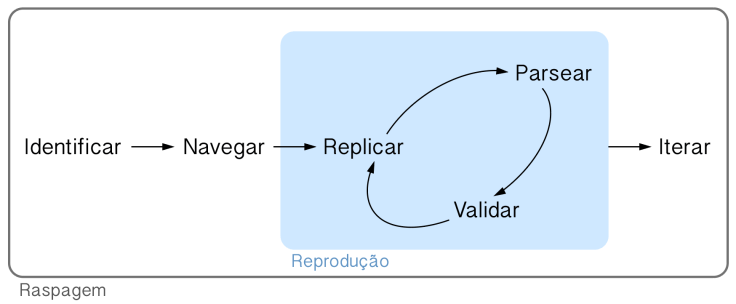
\includegraphics{./assets/img/cycle.png}

}

\caption{\label{fig-fluxo-web-scraping}Ciclo da raspagem de dados.
Fonte: \href{https://curso-r.github.io/main-web-scraping}{curso de Web
Scraping da Curso-R}.}

\end{figure}

No caso da RFB, o trabalho é iniciado acessando-se a
\href{http://servicos.receita.fazenda.gov.br/Servicos/cnpjreva/Cnpjreva_Solicitacao.asp}{página
inicial de busca de CNPJ}, como mostrado na
Figura~\ref{fig-raspagem-rfb-inicial}. É possível notar que o desafio
disponível é do tipo \emph{hCaptcha}, que não é o Captcha de interesse
da pesquisa. No entanto, ao clicar em ``Captcha Sonoro'', é possível
acessar o Captcha de interesse, como mostrado na
Figura~\ref{fig-raspagem-rfb-sonoro}. O motivo pelo qual o Captcha de
texto em imagem foi mantido após a implementação do \emph{hCaptcha} não
foi encontrado.

\begin{figure}

{\centering \includegraphics{./assets/img/raspagem-rfb-inicial.png}

}

\caption{\label{fig-raspagem-rfb-inicial}Página de busca de CNPJ da
RFB.}

\end{figure}

\begin{figure}

{\centering \includegraphics{./assets/img/raspagem-rfb-sonoro.png}

}

\caption{\label{fig-raspagem-rfb-sonoro}Página de busca de CNPJ da RFB,
com Captcha de texto.}

\end{figure}

A segunda tarefa é a de navegar pelo site, registrando as requisições
realizadas pelo navegador para realizar a consulta. Isso envolve abrir o
inspetor de elementos do navegador, na aba Rede (ou \emph{Network}, em
inglês), anotando as requisições que são realizadas.

No exemplo, testamos o CNPJ 13.612.840/0001-57, da Associação Brasileira
de Jurimetria. Ao preencher o CNPJ e o rótulo do Captcha, algumas
requisições aparecem na aba ``Rede'', como mostrado na
Figura~\ref{fig-raspagem-rfb-rede}. A primeira requisição é do tipo
POST\footnote{Existem dois tipos principais de requisição HTTP. A
  requisição GET serve para capturar uma página da internet, enquanto a
  requisição POST serve para enviar dados para o servidor como, um login
  e uma senha. A lista completa de requisições está disponível na
  \href{https://www.rfc-editor.org/rfc/rfc9110.html}{documentação da
  \emph{Internet Engineering Task Force} (IETF)}.}, responsável por
enviar os dados de CNPJ e do rótulo da imagem para o servidor, que
retorna com os dados da empresa.

\begin{figure}

{\centering \includegraphics{./assets/img/raspagem-rfb-rede.png}

}

\caption{\label{fig-raspagem-rfb-rede}Resultado da busca por CNPJ,
mostrando a aba Rede.}

\end{figure}

Investigando a requisição POST, na sub-aba ``Requisição'', é possível
observar os dados da consulta. Trata-se de um conjunto de parâmetros
enviados na forma de lista, com as informações abaixo. Para replicar a
requisição na linguagem de programação, estes são os dados enviados.

\begin{verbatim}
{
    "origem": "comprovante",
    "cnpj": "13.612.840/0001-57",
    "txtTexto_captcha_serpro_gov_br": "7hkhze",
    "search_type": "cnpj"
}
\end{verbatim}

As etapas de replicar, parsear e validar envolvem baixar e processar os
dados na linguagem de programação. No caso do Captcha da RFB, essa
tarefa envolve os passos abaixo.

\begin{enumerate}
\def\labelenumi{\arabic{enumi}.}
\tightlist
\item
  Acessar a página inicial de
  \href{http://servicos.receita.fazenda.gov.br/Servicos/cnpjreva/Cnpjreva_Solicitacao_CS.asp}{busca
  com Captcha sonoro}, através de uma requisição GET.
\item
  Baixar a imagem do Captcha com uma requisição GET, usando o
  \href{http://servicos.receita.fazenda.gov.br/Servicos/cnpjreva/captcha/gerarCaptcha.asp}{link
  gerado} ao clicar no botão de atualizar o Captcha.
\item
  Obter o rótulo a partir da imagem do Captcha.
\item
  Realizar a requisição POST com os dados do exemplo e o rótulo correto
  da imagem, baixando arquivo resultante em um HTML.
\item
  Utilizar técnicas de raspagem de arquivos HTML para obter os dados de
  interesse (como, por exemplo, a razão social da empresa) e validar os
  resultados, verificando, por exemplo, se o resultado estava completo e
  disponível.
\end{enumerate}

Todos os passos descritos acima devem ser realizados em uma sessão
persistente. Isso significa que a biblioteca utilizada para realizar as
requisições deve ser capaz de guardar os \emph{cookies} entre a
requisição GET do primeiro passo e a requisição POST do quarto passo, de
forma que as requisições sejam interligadas.

O quinto passo da lista acima descreve a parte de \emph{parsear,} que é
a responsável pelo nome ``raspagem'' nessa área do conhecimento. O nome
é adequado porque usualmente os arquivos baixados estão em um formato
bruto, inadequado para realização de análises. Os dados precisam ser
então extraídos -- raspados -- do arquivo HTML, através de ferramentas
de transformação de arquivos como a \emph{libxml2} (WICKHAM; HESTER;
OOMS, 2021), técnicas para acessar pedaços do documento, como o XPath
(WICKHAM, 2022a) e técnicas de manipulação de textos, como expressões
regulares (WICKHAM, 2022b).

A iteração encerra o fluxo da raspagem de dados. Nessa etapa, as
operações de replicar, parsear e validar o resultado são reaplicadas
iterativamente, com o fim de baixar dados para compor uma base maior. No
exemplo da RFB, isso significaria montar uma base de dados a partir de
uma lista de CNPJs.

No contexto dos Captchas, o interesse está nos passos de Replicar e
Validar. Estes são os passos em que a imagem é baixado e o rótulo é
anotado e testado no servidor. Esses são os passos relacionados à
anotação manual, e também à implementação do oráculo.

A anotação manual dos Captchas envolve o trabalho de baixar, anotar
(manualmente) e verificar se a anotação está correta. Trata-se de um
trabalho repetitivo e dispendioso, utilizado para gerar as simulações do
trabalho.

O oráculo envolve a possibilidade de checar, de forma automática, se uma
predição do rótulo de uma imagem está correta. Por ser um teste de
Turing inverso, o Captcha é obrigado a mencionar se uma predição está
correta: se a predição foi correta, a página de interesse é acessada; se
a predição está incorreta, o site envia uma mensagem de erro. As etapas
de replicar, parsear e validar para qualquer site de interesse envolvem
os passos a seguir.

\begin{enumerate}
\def\labelenumi{\arabic{enumi}.}
\tightlist
\item
  Acessar a página do site de interesse.
\item
  Preencher o formulário de pesquisa com a informação a ser consultada.
  Por exemplo, no site da RFB, a informação é o CNPJ da empresa a ser
  consultada. Em um site de tribunal, a informação é um número
  identificador de processo.
\item
  Baixar a imagem do Captcha da busca.
\item
  Obter o rótulo da imagem, aplicando um modelo na imagem baixada ou
  anotado manualmente.
\item
  Submeter a consulta no site, informando o rótulo.
\item
  Verificar o resultado. Se acessou a página desejada, o rótulo está
  correto. Caso contrário, o rótulo está incorreto.
\end{enumerate}

O procedimento descrito pode ser reproduzindo indefinidamente. Isso
significa que é possível criar uma base de dados virtualmente infinita
de imagens rotuladas, com a informação adicional do rótulo estar correto
ou incorreto. Isso foi feito para gerar os dados utilizados na
simulação.

O problema do uso de oráculos é que a informação adicional recebida
quando o modelo erra é \textbf{incompleta}. A única informação nova
disponível é que o rótulo testado está incorreto, dentre todos os
rótulos possíveis daquela imagem. Como existe uma grande quantidade de
rótulos possíveis em um Captcha, muitas vezes na ordem de milhões, a
informação que o oráculo fornece é fraca.

Uma possível abordagem para lidar com o segundo problema seria
simplesmente descartar os Captchas classificados incorretamente. É
possível criar uma base de dados (virtualmente infinita) somente com os
rótulos corretos e ajustar um novo modelo. Essa abordagem, no entanto,
tem sérios problemas, já que considera somente os casos em que o
classificador já funciona bem. O trabalho realizado na tese incorpora a
informação fornecida pelo oráculo quando o modelo erra.

Outra oportunidade que o oráculo oferece em parte dos casos é a
possibilidade de testar mais de uma predição. Sites com essa
característica permitem que a pessoa ou robô teste mais de uma predição
caso o Captcha tenha fracassado. Como é possível observar na
Tabela~\ref{tbl-lista-captcha}, dos 10 Captchas trabalhados, 7 permitem
a realização desses testes.

Neste momento, cabe uma observação sobre oráculos e força bruta. O poder
de testar vários rótulos para o mesmo Captcha implica na possibilidade
teórica de resolver um Captcha por força bruta. Bastaria testar todos os
rótulos possíveis para acessar a página de interesse. Na prática, no
entanto, essa estratégia não funciona, já que a quantidade de rótulos
possíveis é muito grande para testar no site, seja por demorar muito
tempo ou pelo site forçar a troca do desafio após a passagem de
determinado tempo ou quantidade de tentativas.

Voltando ao ciclo da raspagem, ao longo do procedimento de baixar
imagens de Captchas e aplicar o oráculo, pelo menos duas funções devem
ser criadas: \textbf{acesso} e \textbf{teste}. A operação de acesso é
responsável por preencher o formulário de busca e baixar o Captcha
(passos 1 a 3 da lista acima). A operação de teste é responsável por
submeter um rótulo do Captcha e verificar retornar se o rótulo está
correto ou incorreto (passos 4 a 6 da lista acima). Em alguns casos, as
funções de acesso e teste precisam compartilhar parâmetros que contêm a
sessão do usuário, para garantir que o teste envolva o mesmo Captcha da
etapa de acesso.

Os Captchas foram anotados manualmente com o procedimento chamado de
semi-automático, definido a seguir. No pacote
\texttt{\{captchaDownload\}} (ver Apêndice \ref{sec-pacote-download}),
foram desenvolvidas ferramentas para baixar e organizar cada Captcha,
utilizando o oráculo para garantir que as imagens eram corretamente
anotadas.

Cada Captcha teve as primeiras 100 observações anotadas manualmente.
Isso foi feito a partir do próprio RStudio, utilizando a ferramenta de
anotação manual do pacote \texttt{\{captcha\}}.

A partir das anotações iniciais, um modelo inicial foi ajustado. Esse
passo também foi feito com o pacote \texttt{\{captcha\}}, que possui uma
função de ajuste de modelos.

O modelo, então, foi utilizado como uma ferramenta para otimizar a
anotação manual, funcionando da seguinte forma. Primeiro, o modelo tenta
realizar a predição automaticamente e o oráculo avisa se a predição está
correta ou não. Se estiver incorreto e o site aceitar várias tentativas,
o modelo tenta novamente, mas com uma segunda alternativa de predição.
Caso o site não aceite várias tentativas ou o modelo não consiga acertar
o Captcha em \(N\) tentativas (abritrado como dez), a imagem do Captcha
aparece para anotação manual.

Com o procedimento destacado acima, é criada uma nova base de dados, que
por sua vez é utilizada para ajustar um novo modelo. O modelo,
atualizado, é utilizado para classificar novos Captchas, e assim por
diante, até que o modelo ajustado alcance uma acurácia razoável, que foi
arbitrada em 80\%. Com isso o procedimento de anotação é finalizado.

O único problema do procedimento de anotação diz respeito aos Captchas
que não aceitam várias tentativas. Nesses casos, não é possível
verificar com certeza absoluta que um caso anotado manualmente (após a
tentativa do modelo) foi anotado corretamente, já que a anotação manual
seria a segunda tentativa. No entanto, esse problema aparece somente em
três Captchas (\texttt{cadesp}, \texttt{jucesp} e \texttt{trf5}). A
anotação manual dos 100 primeiros Captchas, no entanto, mostrou que pelo
menos 95\% dos Captchas foram anotados corretamente quando anotados
manualmente. A proporção máxima de 5\% de erro é negligenciável
considerando que a maior parte das bases de dados foi construída com
verificação do oráculo.

Em alguns casos, os rótulos dos Captchas podem ser obtidos sem
intervenção humana, utilizando técnicas de raspagem de dados e
processamento de sinais. Um exemplo é o Captcha do SEI, que mostra
informações suficientes para resolver o Captcha na própria URL que gera
a imagem. Outro exemplo é o TJMG, que libera, além da imagem, um áudio
contendo o mesmo rótulo da imagem, sem a adição de ruídos. Como o áudio
não tem ruídos, basta ler o áudio, separar os áudios de cada caractere e
calcular uma estatística simples (como a soma das amplitudes, ao
quadrado). Essa estatística é utilizada para associar um pedaço de áudio
a um caractere.

A Tabela~\ref{tbl-lista-captcha-carac} caracteriza os Captchas anotados.
Todos os Captchas possuem comprimento entre 4 e 6 dígitos e, com exceção
do SEI, não são sensíveis a maiúsculas e minúsculas.

\hypertarget{tbl-lista-captcha-carac}{}
\begin{table}[H]

\providecommand{\docline}[3]{\noalign{\global\setlength{\arrayrulewidth}{#1}}\arrayrulecolor[HTML]{#2}\cline{#3}}

\setlength{\tabcolsep}{0pt}

\renewcommand*{\arraystretch}{1.5}

\begin{longtable}[c]{|p{0.75in}|p{0.80in}|p{1.10in}|p{1.10in}|p{0.75in}|p{1.30in}}

\caption{\label{tbl-lista-captcha-carac}Lista de captchas analisados e suas características. } \\ 


\hhline{>{\arrayrulecolor[HTML]{000000}\global\arrayrulewidth=1pt}->{\arrayrulecolor[HTML]{000000}\global\arrayrulewidth=1pt}->{\arrayrulecolor[HTML]{000000}\global\arrayrulewidth=1pt}->{\arrayrulecolor[HTML]{000000}\global\arrayrulewidth=1pt}->{\arrayrulecolor[HTML]{000000}\global\arrayrulewidth=1pt}->{\arrayrulecolor[HTML]{000000}\global\arrayrulewidth=1pt}-}

\multicolumn{1}{!{\color[HTML]{000000}\vrule width 0pt}>{\centering}p{\dimexpr 0.75in+0\tabcolsep+0\arrayrulewidth}}{\textcolor[HTML]{000000}{\fontsize{11}{22}\selectfont{Captcha}}} & \multicolumn{1}{!{\color[HTML]{000000}\vrule width 0pt}>{\centering}p{\dimexpr 0.8in+0\tabcolsep+0\arrayrulewidth}}{\textcolor[HTML]{000000}{\fontsize{11}{22}\selectfont{Vários\ chutes}}} & \multicolumn{1}{!{\color[HTML]{000000}\vrule width 0pt}>{\centering}p{\dimexpr 1.1in+0\tabcolsep+0\arrayrulewidth}}{\textcolor[HTML]{000000}{\fontsize{11}{22}\selectfont{Caracteres}}} & \multicolumn{1}{!{\color[HTML]{000000}\vrule width 0pt}>{\centering}p{\dimexpr 1.1in+0\tabcolsep+0\arrayrulewidth}}{\textcolor[HTML]{000000}{\fontsize{11}{22}\selectfont{Comprimento}}} & \multicolumn{1}{!{\color[HTML]{000000}\vrule width 0pt}>{\centering}p{\dimexpr 0.75in+0\tabcolsep+0\arrayrulewidth}}{\textcolor[HTML]{000000}{\fontsize{11}{22}\selectfont{Colorido}}} & \multicolumn{1}{!{\color[HTML]{000000}\vrule width 0pt}>{\centering}p{\dimexpr 1.3in+0\tabcolsep+0\arrayrulewidth}!{\color[HTML]{000000}\vrule width 0pt}}{\textcolor[HTML]{000000}{\fontsize{11}{22}\selectfont{\#\ Rótulos\ anotados}}} \\

\hhline{>{\arrayrulecolor[HTML]{000000}\global\arrayrulewidth=1pt}->{\arrayrulecolor[HTML]{000000}\global\arrayrulewidth=1pt}->{\arrayrulecolor[HTML]{000000}\global\arrayrulewidth=1pt}->{\arrayrulecolor[HTML]{000000}\global\arrayrulewidth=1pt}->{\arrayrulecolor[HTML]{000000}\global\arrayrulewidth=1pt}->{\arrayrulecolor[HTML]{000000}\global\arrayrulewidth=1pt}-}\endhead



\multicolumn{1}{!{\color[HTML]{000000}\vrule width 0pt}>{\centering}p{\dimexpr 0.75in+0\tabcolsep+0\arrayrulewidth}}{\textcolor[HTML]{000000}{\fontsize{11}{22}\selectfont{\href{https://pje.trf5.jus.br/pje/ConsultaPublica/listView.seam}{trf5}}}} & \multicolumn{1}{!{\color[HTML]{000000}\vrule width 0pt}>{\centering}p{\dimexpr 0.8in+0\tabcolsep+0\arrayrulewidth}}{\textcolor[HTML]{000000}{\fontsize{11}{22}\selectfont{Não}}} & \multicolumn{1}{!{\color[HTML]{000000}\vrule width 0pt}>{\centering}p{\dimexpr 1.1in+0\tabcolsep+0\arrayrulewidth}}{\textcolor[HTML]{000000}{\fontsize{11}{22}\selectfont{0:9}}} & \multicolumn{1}{!{\color[HTML]{000000}\vrule width 0pt}>{\centering}p{\dimexpr 1.1in+0\tabcolsep+0\arrayrulewidth}}{\textcolor[HTML]{000000}{\fontsize{11}{22}\selectfont{6}}} & \multicolumn{1}{!{\color[HTML]{000000}\vrule width 0pt}>{\centering}p{\dimexpr 0.75in+0\tabcolsep+0\arrayrulewidth}}{\textcolor[HTML]{000000}{\fontsize{11}{22}\selectfont{não}}} & \multicolumn{1}{!{\color[HTML]{000000}\vrule width 0pt}>{\centering}p{\dimexpr 1.3in+0\tabcolsep+0\arrayrulewidth}!{\color[HTML]{000000}\vrule width 0pt}}{\textcolor[HTML]{000000}{\fontsize{11}{22}\selectfont{1000}}} \\





\multicolumn{1}{!{\color[HTML]{000000}\vrule width 0pt}>{\centering}p{\dimexpr 0.75in+0\tabcolsep+0\arrayrulewidth}}{\textcolor[HTML]{000000}{\fontsize{11}{22}\selectfont{\href{https://www4.tjmg.jus.br/juridico/sf/proc\_resultado.jsp?comrCodigo=24\&numero=1\&listaProcessos=50718889720218130024\&btn\_pesquisar=Pesquisar}{tjmg}}}} & \multicolumn{1}{!{\color[HTML]{000000}\vrule width 0pt}>{\centering}p{\dimexpr 0.8in+0\tabcolsep+0\arrayrulewidth}}{\textcolor[HTML]{000000}{\fontsize{11}{22}\selectfont{Sim}}} & \multicolumn{1}{!{\color[HTML]{000000}\vrule width 0pt}>{\centering}p{\dimexpr 1.1in+0\tabcolsep+0\arrayrulewidth}}{\textcolor[HTML]{000000}{\fontsize{11}{22}\selectfont{0:9}}} & \multicolumn{1}{!{\color[HTML]{000000}\vrule width 0pt}>{\centering}p{\dimexpr 1.1in+0\tabcolsep+0\arrayrulewidth}}{\textcolor[HTML]{000000}{\fontsize{11}{22}\selectfont{5}}} & \multicolumn{1}{!{\color[HTML]{000000}\vrule width 0pt}>{\centering}p{\dimexpr 0.75in+0\tabcolsep+0\arrayrulewidth}}{\textcolor[HTML]{000000}{\fontsize{11}{22}\selectfont{sim}}} & \multicolumn{1}{!{\color[HTML]{000000}\vrule width 0pt}>{\centering}p{\dimexpr 1.3in+0\tabcolsep+0\arrayrulewidth}!{\color[HTML]{000000}\vrule width 0pt}}{\textcolor[HTML]{000000}{\fontsize{11}{22}\selectfont{1000}}} \\





\multicolumn{1}{!{\color[HTML]{000000}\vrule width 0pt}>{\centering}p{\dimexpr 0.75in+0\tabcolsep+0\arrayrulewidth}}{\textcolor[HTML]{000000}{\fontsize{11}{22}\selectfont{\href{https://pje-consulta.trt3.jus.br/pje-consulta-api/api/processos/2104879}{trt}}}} & \multicolumn{1}{!{\color[HTML]{000000}\vrule width 0pt}>{\centering}p{\dimexpr 0.8in+0\tabcolsep+0\arrayrulewidth}}{\textcolor[HTML]{000000}{\fontsize{11}{22}\selectfont{Sim}}} & \multicolumn{1}{!{\color[HTML]{000000}\vrule width 0pt}>{\centering}p{\dimexpr 1.1in+0\tabcolsep+0\arrayrulewidth}}{\textcolor[HTML]{000000}{\fontsize{11}{22}\selectfont{a-z0:9}}} & \multicolumn{1}{!{\color[HTML]{000000}\vrule width 0pt}>{\centering}p{\dimexpr 1.1in+0\tabcolsep+0\arrayrulewidth}}{\textcolor[HTML]{000000}{\fontsize{11}{22}\selectfont{6}}} & \multicolumn{1}{!{\color[HTML]{000000}\vrule width 0pt}>{\centering}p{\dimexpr 0.75in+0\tabcolsep+0\arrayrulewidth}}{\textcolor[HTML]{000000}{\fontsize{11}{22}\selectfont{não}}} & \multicolumn{1}{!{\color[HTML]{000000}\vrule width 0pt}>{\centering}p{\dimexpr 1.3in+0\tabcolsep+0\arrayrulewidth}!{\color[HTML]{000000}\vrule width 0pt}}{\textcolor[HTML]{000000}{\fontsize{11}{22}\selectfont{1500}}} \\





\multicolumn{1}{!{\color[HTML]{000000}\vrule width 0pt}>{\centering}p{\dimexpr 0.75in+0\tabcolsep+0\arrayrulewidth}}{\textcolor[HTML]{000000}{\fontsize{11}{22}\selectfont{\href{http://esaj.tjba.jus.br/cpopg/open.do}{esaj}}}} & \multicolumn{1}{!{\color[HTML]{000000}\vrule width 0pt}>{\centering}p{\dimexpr 0.8in+0\tabcolsep+0\arrayrulewidth}}{\textcolor[HTML]{000000}{\fontsize{11}{22}\selectfont{Sim}}} & \multicolumn{1}{!{\color[HTML]{000000}\vrule width 0pt}>{\centering}p{\dimexpr 1.1in+0\tabcolsep+0\arrayrulewidth}}{\textcolor[HTML]{000000}{\fontsize{11}{22}\selectfont{a-z}}} & \multicolumn{1}{!{\color[HTML]{000000}\vrule width 0pt}>{\centering}p{\dimexpr 1.1in+0\tabcolsep+0\arrayrulewidth}}{\textcolor[HTML]{000000}{\fontsize{11}{22}\selectfont{5}}} & \multicolumn{1}{!{\color[HTML]{000000}\vrule width 0pt}>{\centering}p{\dimexpr 0.75in+0\tabcolsep+0\arrayrulewidth}}{\textcolor[HTML]{000000}{\fontsize{11}{22}\selectfont{sim}}} & \multicolumn{1}{!{\color[HTML]{000000}\vrule width 0pt}>{\centering}p{\dimexpr 1.3in+0\tabcolsep+0\arrayrulewidth}!{\color[HTML]{000000}\vrule width 0pt}}{\textcolor[HTML]{000000}{\fontsize{11}{22}\selectfont{3000}}} \\





\multicolumn{1}{!{\color[HTML]{000000}\vrule width 0pt}>{\centering}p{\dimexpr 0.75in+0\tabcolsep+0\arrayrulewidth}}{\textcolor[HTML]{000000}{\fontsize{11}{22}\selectfont{\href{https://www.jucesponline.sp.gov.br/ResultadoBusca.aspx}{jucesp}}}} & \multicolumn{1}{!{\color[HTML]{000000}\vrule width 0pt}>{\centering}p{\dimexpr 0.8in+0\tabcolsep+0\arrayrulewidth}}{\textcolor[HTML]{000000}{\fontsize{11}{22}\selectfont{Não}}} & \multicolumn{1}{!{\color[HTML]{000000}\vrule width 0pt}>{\centering}p{\dimexpr 1.1in+0\tabcolsep+0\arrayrulewidth}}{\textcolor[HTML]{000000}{\fontsize{11}{22}\selectfont{a-z0-9}}} & \multicolumn{1}{!{\color[HTML]{000000}\vrule width 0pt}>{\centering}p{\dimexpr 1.1in+0\tabcolsep+0\arrayrulewidth}}{\textcolor[HTML]{000000}{\fontsize{11}{22}\selectfont{5}}} & \multicolumn{1}{!{\color[HTML]{000000}\vrule width 0pt}>{\centering}p{\dimexpr 0.75in+0\tabcolsep+0\arrayrulewidth}}{\textcolor[HTML]{000000}{\fontsize{11}{22}\selectfont{não}}} & \multicolumn{1}{!{\color[HTML]{000000}\vrule width 0pt}>{\centering}p{\dimexpr 1.3in+0\tabcolsep+0\arrayrulewidth}!{\color[HTML]{000000}\vrule width 0pt}}{\textcolor[HTML]{000000}{\fontsize{11}{22}\selectfont{4000}}} \\





\multicolumn{1}{!{\color[HTML]{000000}\vrule width 0pt}>{\centering}p{\dimexpr 0.75in+0\tabcolsep+0\arrayrulewidth}}{\textcolor[HTML]{000000}{\fontsize{11}{22}\selectfont{\href{https://srv01.tjpe.jus.br/consultaprocessualunificada/}{tjpe}}}} & \multicolumn{1}{!{\color[HTML]{000000}\vrule width 0pt}>{\centering}p{\dimexpr 0.8in+0\tabcolsep+0\arrayrulewidth}}{\textcolor[HTML]{000000}{\fontsize{11}{22}\selectfont{Sim}}} & \multicolumn{1}{!{\color[HTML]{000000}\vrule width 0pt}>{\centering}p{\dimexpr 1.1in+0\tabcolsep+0\arrayrulewidth}}{\textcolor[HTML]{000000}{\fontsize{11}{22}\selectfont{a-z0-9}}} & \multicolumn{1}{!{\color[HTML]{000000}\vrule width 0pt}>{\centering}p{\dimexpr 1.1in+0\tabcolsep+0\arrayrulewidth}}{\textcolor[HTML]{000000}{\fontsize{11}{22}\selectfont{5}}} & \multicolumn{1}{!{\color[HTML]{000000}\vrule width 0pt}>{\centering}p{\dimexpr 0.75in+0\tabcolsep+0\arrayrulewidth}}{\textcolor[HTML]{000000}{\fontsize{11}{22}\selectfont{não}}} & \multicolumn{1}{!{\color[HTML]{000000}\vrule width 0pt}>{\centering}p{\dimexpr 1.3in+0\tabcolsep+0\arrayrulewidth}!{\color[HTML]{000000}\vrule width 0pt}}{\textcolor[HTML]{000000}{\fontsize{11}{22}\selectfont{4000}}} \\





\multicolumn{1}{!{\color[HTML]{000000}\vrule width 0pt}>{\centering}p{\dimexpr 0.75in+0\tabcolsep+0\arrayrulewidth}}{\textcolor[HTML]{000000}{\fontsize{11}{22}\selectfont{\href{https://www.tjrs.jus.br/site\_php/consulta/verificador.php}{tjrs}}}} & \multicolumn{1}{!{\color[HTML]{000000}\vrule width 0pt}>{\centering}p{\dimexpr 0.8in+0\tabcolsep+0\arrayrulewidth}}{\textcolor[HTML]{000000}{\fontsize{11}{22}\selectfont{Sim}}} & \multicolumn{1}{!{\color[HTML]{000000}\vrule width 0pt}>{\centering}p{\dimexpr 1.1in+0\tabcolsep+0\arrayrulewidth}}{\textcolor[HTML]{000000}{\fontsize{11}{22}\selectfont{0-9}}} & \multicolumn{1}{!{\color[HTML]{000000}\vrule width 0pt}>{\centering}p{\dimexpr 1.1in+0\tabcolsep+0\arrayrulewidth}}{\textcolor[HTML]{000000}{\fontsize{11}{22}\selectfont{4}}} & \multicolumn{1}{!{\color[HTML]{000000}\vrule width 0pt}>{\centering}p{\dimexpr 0.75in+0\tabcolsep+0\arrayrulewidth}}{\textcolor[HTML]{000000}{\fontsize{11}{22}\selectfont{sim}}} & \multicolumn{1}{!{\color[HTML]{000000}\vrule width 0pt}>{\centering}p{\dimexpr 1.3in+0\tabcolsep+0\arrayrulewidth}!{\color[HTML]{000000}\vrule width 0pt}}{\textcolor[HTML]{000000}{\fontsize{11}{22}\selectfont{2000}}} \\





\multicolumn{1}{!{\color[HTML]{000000}\vrule width 0pt}>{\centering}p{\dimexpr 0.75in+0\tabcolsep+0\arrayrulewidth}}{\textcolor[HTML]{000000}{\fontsize{11}{22}\selectfont{\href{https://www.cadesp.fazenda.sp.gov.br/(S(vyfz1cfybbxj3sgpf4eqhxd3}{cadesp}}}} & \multicolumn{1}{!{\color[HTML]{000000}\vrule width 0pt}>{\centering}p{\dimexpr 0.8in+0\tabcolsep+0\arrayrulewidth}}{\textcolor[HTML]{000000}{\fontsize{11}{22}\selectfont{Não}}} & \multicolumn{1}{!{\color[HTML]{000000}\vrule width 0pt}>{\centering}p{\dimexpr 1.1in+0\tabcolsep+0\arrayrulewidth}}{\textcolor[HTML]{000000}{\fontsize{11}{22}\selectfont{a-z}}} & \multicolumn{1}{!{\color[HTML]{000000}\vrule width 0pt}>{\centering}p{\dimexpr 1.1in+0\tabcolsep+0\arrayrulewidth}}{\textcolor[HTML]{000000}{\fontsize{11}{22}\selectfont{4}}} & \multicolumn{1}{!{\color[HTML]{000000}\vrule width 0pt}>{\centering}p{\dimexpr 0.75in+0\tabcolsep+0\arrayrulewidth}}{\textcolor[HTML]{000000}{\fontsize{11}{22}\selectfont{sim}}} & \multicolumn{1}{!{\color[HTML]{000000}\vrule width 0pt}>{\centering}p{\dimexpr 1.3in+0\tabcolsep+0\arrayrulewidth}!{\color[HTML]{000000}\vrule width 0pt}}{\textcolor[HTML]{000000}{\fontsize{11}{22}\selectfont{3000}}} \\





\multicolumn{1}{!{\color[HTML]{000000}\vrule width 0pt}>{\centering}p{\dimexpr 0.75in+0\tabcolsep+0\arrayrulewidth}}{\textcolor[HTML]{000000}{\fontsize{11}{22}\selectfont{\href{https://sei.economia.gov.br/sei/modulos/pesquisa/md\_pesq\_processo\_pesquisar.php?acao\_externa=protocolo\_pesquisar\&acao\_origem\_externa=protocolo\_pesquisar\&id\_orgao\_acesso\_externo=0}{sei}}}} & \multicolumn{1}{!{\color[HTML]{000000}\vrule width 0pt}>{\centering}p{\dimexpr 0.8in+0\tabcolsep+0\arrayrulewidth}}{\textcolor[HTML]{000000}{\fontsize{11}{22}\selectfont{Sim}}} & \multicolumn{1}{!{\color[HTML]{000000}\vrule width 0pt}>{\centering}p{\dimexpr 1.1in+0\tabcolsep+0\arrayrulewidth}}{\textcolor[HTML]{000000}{\fontsize{11}{22}\selectfont{a-zA-Z0-9}}} & \multicolumn{1}{!{\color[HTML]{000000}\vrule width 0pt}>{\centering}p{\dimexpr 1.1in+0\tabcolsep+0\arrayrulewidth}}{\textcolor[HTML]{000000}{\fontsize{11}{22}\selectfont{4}}} & \multicolumn{1}{!{\color[HTML]{000000}\vrule width 0pt}>{\centering}p{\dimexpr 0.75in+0\tabcolsep+0\arrayrulewidth}}{\textcolor[HTML]{000000}{\fontsize{11}{22}\selectfont{sim}}} & \multicolumn{1}{!{\color[HTML]{000000}\vrule width 0pt}>{\centering}p{\dimexpr 1.3in+0\tabcolsep+0\arrayrulewidth}!{\color[HTML]{000000}\vrule width 0pt}}{\textcolor[HTML]{000000}{\fontsize{11}{22}\selectfont{10000}}} \\





\multicolumn{1}{!{\color[HTML]{000000}\vrule width 0pt}>{\centering}p{\dimexpr 0.75in+0\tabcolsep+0\arrayrulewidth}}{\textcolor[HTML]{000000}{\fontsize{11}{22}\selectfont{\href{https://servicos.receita.fazenda.gov.br/servicos/cnpjreva/Cnpjreva\_Solicitacao\_CS.asp}{rfb}}}} & \multicolumn{1}{!{\color[HTML]{000000}\vrule width 0pt}>{\centering}p{\dimexpr 0.8in+0\tabcolsep+0\arrayrulewidth}}{\textcolor[HTML]{000000}{\fontsize{11}{22}\selectfont{Sim}}} & \multicolumn{1}{!{\color[HTML]{000000}\vrule width 0pt}>{\centering}p{\dimexpr 1.1in+0\tabcolsep+0\arrayrulewidth}}{\textcolor[HTML]{000000}{\fontsize{11}{22}\selectfont{a-z0-9}}} & \multicolumn{1}{!{\color[HTML]{000000}\vrule width 0pt}>{\centering}p{\dimexpr 1.1in+0\tabcolsep+0\arrayrulewidth}}{\textcolor[HTML]{000000}{\fontsize{11}{22}\selectfont{6}}} & \multicolumn{1}{!{\color[HTML]{000000}\vrule width 0pt}>{\centering}p{\dimexpr 0.75in+0\tabcolsep+0\arrayrulewidth}}{\textcolor[HTML]{000000}{\fontsize{11}{22}\selectfont{não}}} & \multicolumn{1}{!{\color[HTML]{000000}\vrule width 0pt}>{\centering}p{\dimexpr 1.3in+0\tabcolsep+0\arrayrulewidth}!{\color[HTML]{000000}\vrule width 0pt}}{\textcolor[HTML]{000000}{\fontsize{11}{22}\selectfont{4000}}} \\

\hhline{>{\arrayrulecolor[HTML]{000000}\global\arrayrulewidth=1pt}->{\arrayrulecolor[HTML]{000000}\global\arrayrulewidth=1pt}->{\arrayrulecolor[HTML]{000000}\global\arrayrulewidth=1pt}->{\arrayrulecolor[HTML]{000000}\global\arrayrulewidth=1pt}->{\arrayrulecolor[HTML]{000000}\global\arrayrulewidth=1pt}->{\arrayrulecolor[HTML]{000000}\global\arrayrulewidth=1pt}-}



\end{longtable}

\end{table}

As bases de dados com imagens anotadas foram disponibilizadas na aba de
lançamentos (\emph{releases}) do
\href{https://github.com/jtrecenti/doutorado/releases}{repositório
principal do projeto de pesquisa}. As bases com imagens e modelos
ajustados estão disponíveis para quem tiver interesse em fazer novas
pesquisas e utilizar os resultados em suas aplicações, sem restrições de
uso.

\hypertarget{simulacoes}{%
\section{Simulações}\label{simulacoes}}

Para verificar o poder do uso do oráculo para o aprendizado do modelo,
uma série de simulações foi desenvolvidas. As simulações foram
organizadas em três passos: modelo inicial, dados e modelo final. Os
passos foram descritos em maior detalhe a seguir.

\hypertarget{primeiro-passo-modelo-inicial}{%
\subsection{Primeiro passo: modelo
inicial}\label{primeiro-passo-modelo-inicial}}

A simulação do modelo inicial teve como objetivo obter modelos
preditivos de Captchas com acurácias distintas. O modelo inicial seria
usado, então, para baixar dados diretamente do site usando o oráculo e,
por fim, ajustar um modelo final com os novos dados provenientes do
oráculo.

Os modelos iniciais foram construídos em dois passos. O primeiro foi
montar a base de dados completa, suficiente para ajustar um modelo com
alta acurácia, que arbitrados em 80\%, como descrito anteriormente.
Depois, montou-se 10 amostras de dados com subconjuntos das bases
completas, cada uma contendo 10\%, 20\%, e assim por diante, até a base
completa. Por exemplo: no Captcha da Jucesp, construiu-se um modelo com
acurácia maior que 80\% com 4000 Captchas. A partir disso, foi feita uma
partição dos dados com 400 imagens (10\% do total), 800 imagens (20\% do
total) e assim por diante, até o modelo com 4000 Captchas.

Para cada tamanho de amostra \(A\), aplicou-se uma bateria de 27
modelos. Isso foi feito porque para diferentes quantidades de amostra, a
configuração dos hiperparâmetros que resulta no melhor modelo pode ser
diferente. Os modelos seguiram uma grade de hiperparâmetros considerando
três informações:

\begin{itemize}
\tightlist
\item
  A quantidade de unidades computacionais na primeira camada densa após
  as camadas convolucionais, com os valores considerados: 100, 200 e
  300.
\item
  O valor do \emph{dropout} aplicado às camadas densas, com os valores
  considerados: 10\%, 30\% e 50\%.
\item
  O fator de decaimento na taxa de aprendizado a cada época, com os
  valores considerados: 1\%, 2\% e 3\%.
\end{itemize}

Combinando os três valores dos três hiperparâmetros, tem-se um total de
\(27=3^3\) hiperparâmetros. Com isso, foi possível identificar, para
cada tamanho de amostra \(A\), o classificador \(C_A\) com a melhor
acurácia dentre os modelos ajustados.

No final do primeiro passo, portanto, considera-se apenas o melhor
modelo para cada tamanho de amostra, dentre os 27 ajustados. É claro que
os modelos encontrados por essa técnica não são, necessariamente, os
melhores modelos possíveis. No entanto, como a técnica é a mesma para
todos os Captchas, é possível fazer comparações através de uma
metodologia mais transparente.

\hypertarget{segundo-passo-dados}{%
\subsection{Segundo passo: dados}\label{segundo-passo-dados}}

O segundo passo teve como objetivo construir as bases de dados
utilizando o oráculo. Primeiro, foi necessário decidir quais modelos,
dentre os 10 ajustados para cada Captcha, seriam utilizados para
construir novas bases. Não faria sentido, por exemplo, considerar um
modelo com acurácia de 0\%, já que ele não produziria nenhuma observação
comparado com um modelo que chuta aleatoriamente. Também não faria
sentido considerar um classificador com acurácia de 100\%, já que nesse
caso não há o que testar com a técnica do oráculo.

Decidiu-se que seria necessário considerar somente os modelos que
resultaram em acurácias maiores de 1\% e menores de 50\%. O valor máximo
foi decidido após realizar alguns testes empíricos e verificar,
informalmente, que a técnica do oráculo realmente resultava em ganhos
expressivos, mesmo com modelos de baixa acurácia. Concluiu-se então que
não seria necessário testar a eficácia da técnica para classificadores
com alta acurácia. Já o valor mínimo foi decidido de forma arbitrária,
retirando-se os classificadores com acurácia muito baixa.

A segunda decisão a ser tomada para construção dos dados foi a
quantidade de imagens que seria baixada para cada Captcha. Como são
Captchas de diferentes dificuldades, a quantidade de dados seria
diferente. Optou-se por baixar a quantidade de dados de forma a montar
uma base de treino que contém a quantidade de observações necessária
para obter o melhor modelo daquele Captcha. Por exemplo, no TJRS, um
modelo com acurácia próxima de 100\% foi identificado com 2000
observações. O melhor modelo com 300 imagens (240 para treino, 60 para
teste) resultou em uma acurácia de 35\%. Foram, então, baixadas 1760
observações para compor o total de 2000 na base de treino. As imagens de
teste do modelo inicial poderiam até ser utilizadas, mas optamos por
descartar para garantir que o modelo não ficasse sobreajustado para a
primeira base.

O motivo de baixar a mesma quantidade de observações que o melhor modelo
inicial foi feita por dois motivos. O primeiro é que existem evidências
de que é possível construir um bom modelo com essa quantidade de
imagens, ainda que em um caso as informações são completas e, no outro,
incompletas. O segundo é que isso permite a comparação do resultado do
modelo completamente anotado contra o modelo que é parcialmente anotado
e com anotações incompletas provenientes do oráculo.

A terceira e última decisão tomada para baixar os dados foi a quantidade
de chutes que o modelo poderia fazer, nos casos em que isso é permitido
pelo site. Optou-se, de forma arbitrária, por três valores: 1, que é
equivalente a um site que não permite múltiplos chutes, 5 chutes e 10
chutes.

Portanto, o procedimento de coleta dos dados foi feito, para cada
Captcha, da seguinte forma:

\begin{enumerate}
\def\labelenumi{\arabic{enumi}.}
\tightlist
\item
  Listou-se todos os melhores modelos ajustados para cada tamanho de
  amostra.
\item
  Filtrou-se os modelos para os que apresentavam acurácia de 5\% até
  50\%
\item
  Definiu-se o tamanho da base a ser obtida, com base no tamanho da base
  de treino utilizada no modelo e a quantidade total que se objetivou
  obter.
\item
  Para cada quantidade de tentativas disponível (1, 5 e 10), baixou-se
  as imagens, anotando com o valor ``1'' se o rótulo de alguma das
  tentativas estivesse correto e com o valor ``0'' caso contrário.
\item
  Nos casos com erros, armazenou-se um arquivo de log para cada Captcha
  com o histórico de tentativas incorretas, que é a informação mais
  importante a ser passada para o modelo final.
\end{enumerate}

No final, obteve-se bases de dados de treino para todos os Captchas
analisados, com quantidades de imagens variadas de acordo com os
parâmetros definidos anteriormente, variando também pela quantidade de
tentativas. A quantidade total de bases de dados geradas foi 65.

Além das bases de treino, foi construída uma base de teste para cada
Captcha. As bases de teste foram construídas completamente do zero, sem
utilizar informações de bases anteriores. Para construir as bases,
utilizou-se a mesma técnica semi-automática definida anteriormente,
usando o melhor modelo disponível para classificar a maioria das imagens
e classificando manualmente em caso de falha. Em alguns casos, como TJMG
e TJRS, a anotação humana quase não foi necessária, pois os
classificadores obtidos apresentaram acurácia próxima de 100\%.

Como o único objetivo da base de teste foi o de estimar a acurácia dos
modelos finais, a quantidade de observações poderia ser arbitrada. O
tamanho das bases de teste foi, então, arbitrado em 1000 imagens para
cada Captcha.

\hypertarget{sec-modelo-final}{%
\subsection{Terceiro passo: modelo final}\label{sec-modelo-final}}

O modelo final foi ajustado para cada uma das 65 bases de treino
disponíveis após a realização dos passos 1 e 2. Nesse caso, utilizou-se
o modelo proposto na Seção~\ref{sec-wawl}. Caso a imagem tenha sido
corretamente anotada, a função de perda é calculada normalmente. Caso
ela tenha sido anotada incorretamente, considera-se a probabilidade de
não observar nenhum dos chutes.

Além de modificar a forma de calcular a função de perda do modelo, foi
necessário realizar uma nova busca de hiperparâmetros. Optou-se por
utilizar os mesmos hiperparâmetros dos modelos iniciais para manter a
consistência. O único detalhe nesse ponto é que, como os parâmetros de
partida são os do modelo inicial, optou-se por não modificar a
quantidade de unidades na camada densa, variando somente os valores de
\emph{dropout} e de decaimento na taxa de aprendizado. Portanto,
ajustou-se 9 e não 27 modelos para cada base de dados.

No final, assim como no primeiro passo, os classificadors com melhor
acurácia foram selecionados para cada modelo. Obteve-se, então, com 65
modelos no final para comparar com os modelos iniciais e estimar a
efetividade do oráculo. As comparações foram feitas através de gráficos
de barras, explorando o efeito do uso do oráculo para diferentes
Captchas, diferentes modelos iniciais e diferentes quantidades de
chutes, além de um gráfico de dispersão para relacionar as acurácias
iniciais e finais.

Além do terceiro passo, outros experimentos foram realizados para
verificar se, ao aplicar a técnica do oráculo iterativamente, os
resultados continuariam melhorando. Ou seja, é possível considerar os
modelos obtidos no passo 3 como os modelos iniciais do passo 1, aplicar
novamente o passo 2 (baixar dados) e o passo 3 (rodar modelo com os
novos dados). Isso foi feito para apenas um conjunto selecionado de
Captchas para verificar essa possibilidade, não fazendo parte das
simulações principais do estudo.

As bases de dados das simulações também foram disponibilizadas na aba de
lançamentos (\emph{releases}) do
\href{https://github.com/jtrecenti/doutorado/releases}{repositório
principal do projeto de pesquisa}. As bases podem ser utilizadas para
aumentar as bases de treino e para testar outras arquiteturas de redes
neurais ao tema dos Captchas com uso de aprendizado fracamente
supervisionado.

\bookmarksetup{startatroot}

\hypertarget{sec-results}{%
\chapter{Resultados}\label{sec-results}}

\epigrafe{I'm not a robot, I'm a human. But I'm pretty sure the robot is better at this than I am.}{ChatGPT}

Neste capítulo, discute-se os resultados empíricos do método WAWL e
descreve-se pacote computacional desenvolvido para lidar com Captchas. A
Seção~\ref{sec-result-sim} mostra os resultados empíricos e a
Seção~\ref{sec-pacote-captcha} detalha o pacote \texttt{\{captcha\}}. No
final, a Seção~\ref{sec-discussao} apresenta uma discussão dos
resultados obtidos.

\hypertarget{sec-result-sim}{%
\section{Resultados empíricos}\label{sec-result-sim}}

Os resultados foram obtidos a partir das simulações com diversos
Captchas. Foram realizadas 65 simulações no total, variando no tipo de
Captcha, a acurácia do modelo inicial e a quantidade de tentativas no
oráculo.

Para realizar os cálculos, montou-se uma base de dados com os resultados
das simulações. A base está disponível publicamente no
\href{https://github.com/jtrecenti/doutorado}{repositório da tese} e
contém informações do Captcha ajustado (\texttt{captcha}), da quantidade
de observações do modelo inicial (\texttt{n}), da quantidade de
tentativas do oráculo (\texttt{ntry}), da etapa de simulação
(\texttt{fase}, inicial ou WAWL), do caminho do modelo ajustado
(\texttt{model}) e da acurácia obtida (\texttt{acc}).

Os resultados gerais mostram um ganho de 333\% na acurácia após a
aplicação da metodologia WAWL. Ou seja, em média, a acurácia do modelo
no terceiro passo da simulação (ver Seção~\ref{sec-modelo-final}) foi de
mais de \textbf{três vezes} a acurácia do modelo inicial. Em termos
absolutos (diferença entre as acurácias), o ganho foi de 33\%, ou seja,
após o terceiro passo modelos ganharam, em média, 33\% de acurácia.

As Figuras~\ref{fig-simulacao-geral-ntry-relativo} e
\ref{fig-simulacao-geral-ntry-absoluto} mostram os ganhos relativos e
absolutos, separando os resultados gerais por quantidade de tentativas.
Cada ponto é o resultado de uma simulação e o ponto em destaque é o
valor médio, acompanhado de intervalo \(m \mp 2*s/\sqrt(n)\), com \(m\)
sendo a média, \(s\) o desvio padrão e \(n\) a quantidade de dados. A
linha pontilhada indica se a acurácia aumentou ou diminuiu após a
aplicação da técnica.

Na Figura~\ref{fig-simulacao-geral-ntry-relativo}, é possível notar que
os ganhos em acurácia apresentam alta variabilidade, mas que apresentam
uma tendência positiva com relação ao número de tentativas. O ganho
entre aplicar 5 e 10 tentativas é menos expressivo do que o ganho entre
aplicar 1 e 5 tentativas, indicando que a oportunidade oferecida por
sites que aceitam vários chutes é relevante e que não há necessidade de
realizar tantos chutes para aproveitar essa oportunidade.

\begin{figure}

{\centering 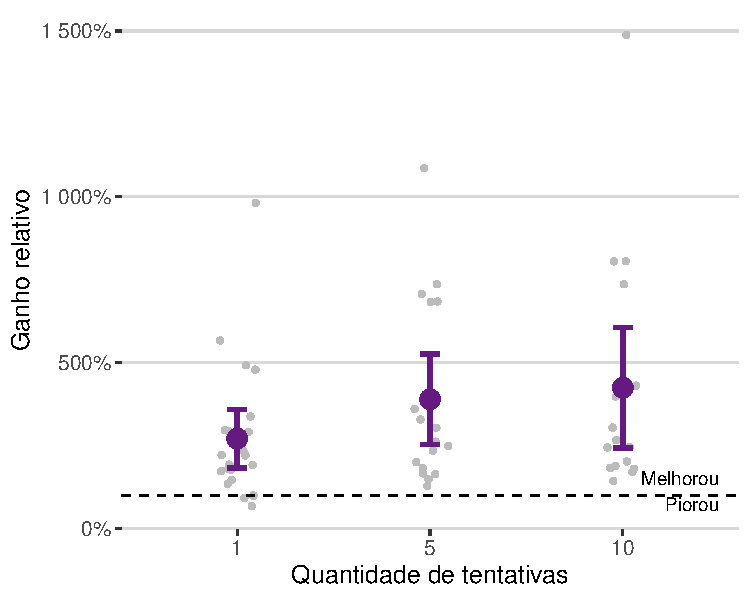
\includegraphics[width=0.75\textwidth,height=\textheight]{./resultados_files/figure-pdf/fig-simulacao-geral-ntry-relativo-1.pdf}

}

\caption{\label{fig-simulacao-geral-ntry-relativo}Ganho percentual ao
utilizar a técnica do oráculo, dividido por quantidade de tentativas.}

\end{figure}

A Figura Figura~\ref{fig-simulacao-geral-ntry-absoluto}, com as os
ganhos absolutos, mostra a mesma informação mas em quantidades mais
fáceis de interpretar. O ganho médio absoluto em sites que permitem mais
de um chute ficou em torno de 40\%, enquanto que o ganho com apenas um
chute ficou um pouco acima de 25\%. Importante notar também que o uso do
oráculo só piorou a acurácia do model em casos que com apenas um chute,
mostrando que a técnica é efetiva de forma consistente.

\begin{figure}

{\centering 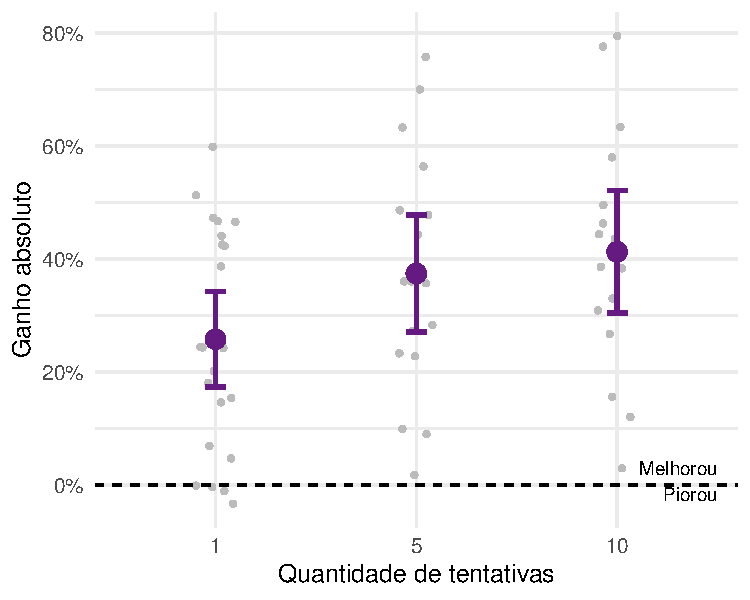
\includegraphics[width=0.75\textwidth,height=\textheight]{./resultados_files/figure-pdf/fig-simulacao-geral-ntry-absoluto-1.pdf}

}

\caption{\label{fig-simulacao-geral-ntry-absoluto}Ganhos absolutos ao
utilizar a técnica do oráculo, dividido por quantidade de tentativas.}

\end{figure}

As Figuras~\ref{fig-simulacao-geral-inicial-relativo} e
\ref{fig-simulacao-geral-inicial-absoluto} apresentam os resultados
gerais separando por acurácia inicial do modelo. A estrutura do gráfico
é similar às visualizações anteriores, que separaram os resultados por
quantidade de tentativas. As categorias escolhidas foram: até 10\%, mais
de 10\% até 35\% e mais de 35\% de acurácia no modelo inicial. A escolha
dos intervalos se deram pela quantidade de observações em cada
categoria.

A Figura~\ref{fig-simulacao-geral-inicial-relativo} mostra os ganhos
relativos. É possível notar uma tendência de queda no ganho de acurácia
com uso do oráculo conforme aumenta a acurácia do modelo inicial. Esse
resultado é esperado, pois, como a acurácia é um número entre zero e um,
um modelo que já possui alta acurácia não tem a possibilidade de
aumentar muito de forma absoluta.

\begin{figure}

{\centering 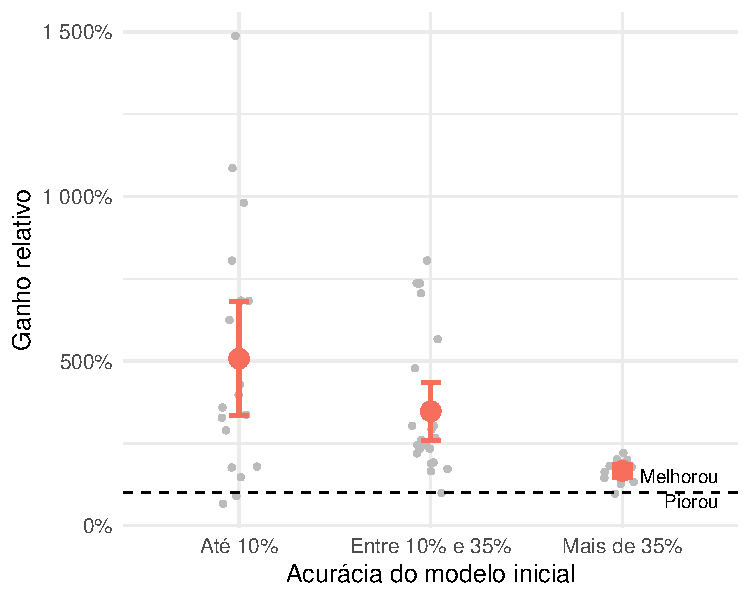
\includegraphics[width=0.75\textwidth,height=\textheight]{./resultados_files/figure-pdf/fig-simulacao-geral-inicial-relativo-1.pdf}

}

\caption{\label{fig-simulacao-geral-inicial-relativo}Ganho percentual ao
utilizar a técnica do oráculo, dividido por acurácia do modelo inicial.}

\end{figure}

A Figura~\ref{fig-simulacao-geral-inicial-absoluto} mostra os ganhos
absolutos. O gráfico apresenta o mesmo problema que o anterior, já que o
ganho máximo depende da acurácia inicial do modelo. Ainda assim, é
possível notar que, em termos absolutos, modelos com acurácia inicial
entre 10\% e 35\% apresentaram um ganho maior que modelos com acurácia
inicial de até 10\%.

\begin{figure}

{\centering 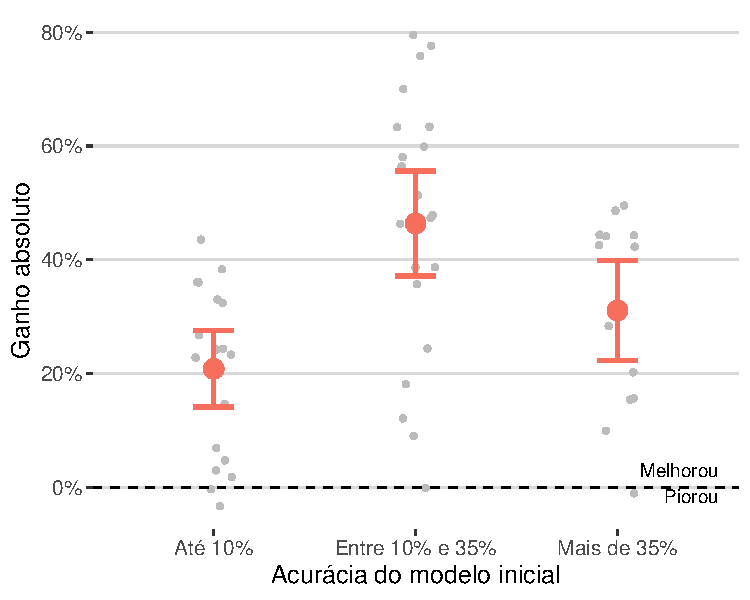
\includegraphics[width=0.75\textwidth,height=\textheight]{./resultados_files/figure-pdf/fig-simulacao-geral-inicial-absoluto-1.pdf}

}

\caption{\label{fig-simulacao-geral-inicial-absoluto}Ganho absoluto ao
utilizar a técnica do oráculo, dividido por acurácia do modelo inicial.}

\end{figure}

Para lidar com o fato da acurácia ser um número limitado, fizemos o
mesmo gráficos de antes, mas ajustado pelo máximo possível que a técnica
do oráculo poderia proporcionar. O ganho absoluto ajustado de uma
simulação é dado por

\[
\text{ganho} = \frac{\text{oráculo } - \text{ inicial}}{1\; - \text{ inicial}}.
\]

A Figura~\ref{fig-simulacao-geral-inicial-absoluto-ajustado} mostra os
ganhos ajustados. Pelo gráfico, é possível notar que existe um ganho
expressivo da técnica WAWL do oráculo para modelos iniciais com mais de
10\% de acurácia com relação a modelos iniciais com até 10\% de
acurácia. Ou seja, quando o modelo inicial é fraco, o ganho ao usar a
técnica é menor. É importante notar, no entanto, que as simulações
mostram a aplicação da técnica apenas uma vez -- é possível baixar mais
dados e atualizar o modelo indefinidamente. O menor efeito da técnica
para modelos iniciais fracos não significa, portanto, que a técnica não
funciona para modelos iniciais fracos; pelo contrário: ela ajuda o
modelo a sair do estado inicial e o leva para um estado com acurácia
maior, de onde seria possível aplicar a técnica novamente para obter
resultads mais expressivos.

\begin{figure}

{\centering 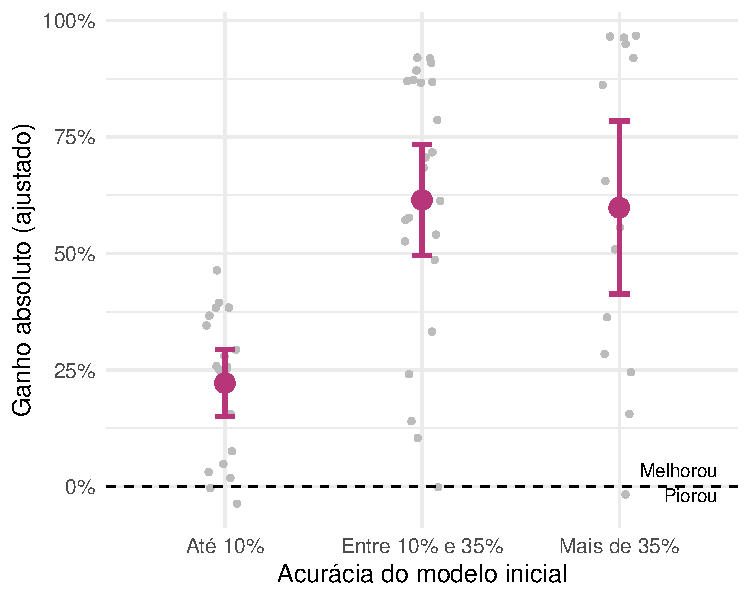
\includegraphics[width=0.75\textwidth,height=\textheight]{./resultados_files/figure-pdf/fig-simulacao-geral-inicial-absoluto-ajustado-1.pdf}

}

\caption{\label{fig-simulacao-geral-inicial-absoluto-ajustado}Ganho
absoluto ao utilizar a técnica do oráculo, dividido por acurácia do
modelo inicial.}

\end{figure}

Na Figura~\ref{fig-simulacao-captcha}, são apresentados os resultados
separando por Captcha. Cada linha é uma combinação de Captcha,
quantidade de tentativas e acurácia modelo inicial, classificados nas
três categorias mostradas anteriormente. As linhas pontilhadas indicam
modelos ajustados com mais de uma tentativa, enquanto as linhas
contínuas mostram modelos ajustados com apenas uma tentativa. A primeira
extremidade de cada linha, do lado esquerdo, indica a acurácia do modelo
inicial e a segunda extremidade, do lado direito, a acurácia do modelo
usando o método WAWL.

\begin{figure}

{\centering 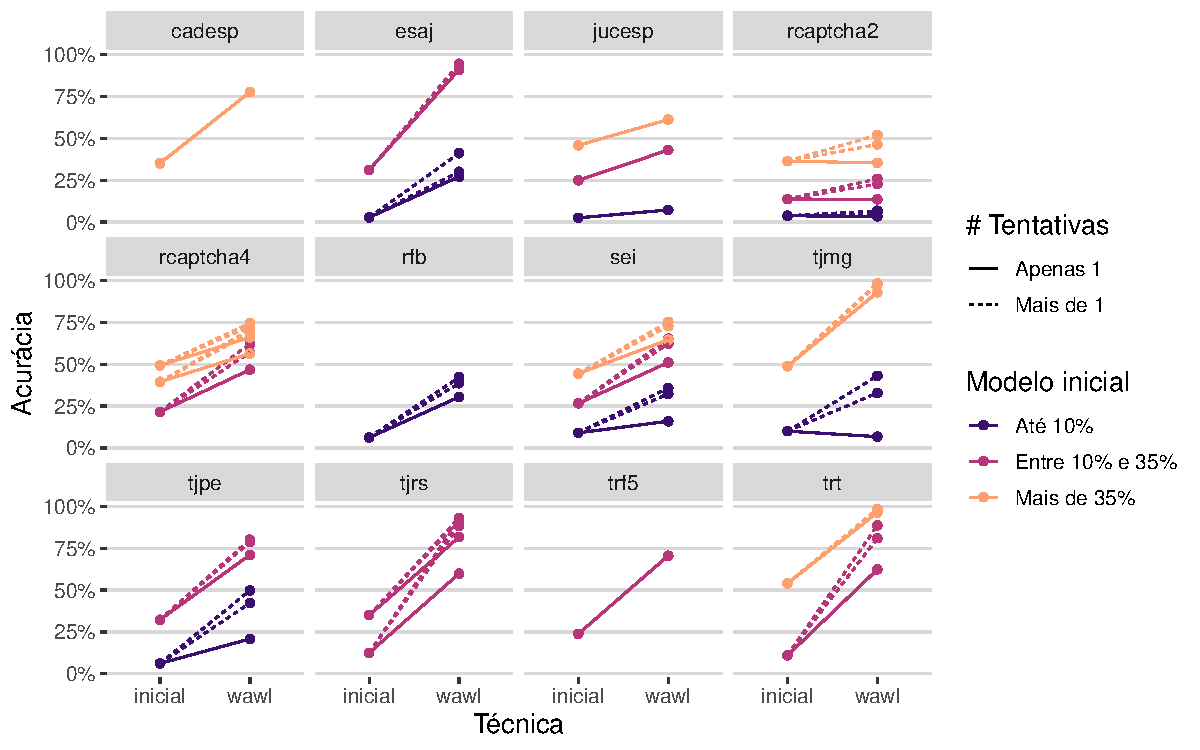
\includegraphics[width=1\textwidth,height=\textheight]{./resultados_files/figure-pdf/fig-simulacao-captcha-1.pdf}

}

\caption{\label{fig-simulacao-captcha}Resultados da simulação por
captcha, quantidade de tentativas e modelo inicial.}

\end{figure}

Pelo gráfico, é possível identificar duas informações relevantes. Como
já verificado anteriormente, os modelos ajustados com mais de uma
tentativa apresentam maiores ganhos do que os modelos ajustados com
apenas uma tentativa. Verifica-se também que modelos com acurácia
inicial de até 10\% só apresentam ganhos menores que os modelos com
acurácia inicial maior que 10\% nos casos em que apenas uma tentativa é
definda. Ou seja, existe interação entre a quantidade de tentativas e a
acurácia do modelo inicial ao avaliar o impacto nos ganhos empíricos do
método WAWL.

Pelos resultados das simulações, é possível concluir que o método WAWL
foi bem sucedido. Primeiro, o método apresenta resultados expressivos e
de forma consistente, sem realizar novas anotações manuais. Além disso,
a técnica aproveita a oportunidade oferecida pelos sites de obter o
\emph{feedback} oráculo múltiplas vezes na mesma imagem. Finalmente, o
método apresenta, em média, resultados positivos mesmo para modelos
iniciais muito fracos (com acurácia de até 10\%), indicando que sua
aplicação é possível para qualquer modelo inicial, o que é bastante
factível de atingir com bases pequenas ou com modelos generalistas para
resolver Captchas.

Um possível problema em aplicar o WAWL é que a técnica poderia
introduzir viés de seleção no modelo, impedindo-o de ser aprimorado
indefinidamente. Mesmo que os resultados teóricos dêem uma boa base para
acreditar que isso não seja verdade, foi feito um experimento adicional,
com apenas um dos Captchas, para verificar se a aplicação da técnica
múltiplas vezes apresenta bons resultados.

O Captcha escolhido para a simulação foi o \texttt{trf5}, por ser um
Captcha que não aceita múltiplos chutes, em uma tentativa de obter um
pior caso. Para esse Captcha, o melhor modelo obtido com a técnica do
oráculo foi considerado como modelo inicial, sendo usado para baixar
novos dados do site do Tribunal. Os novos dados foram adicionados à base
de treino, ajustando-se um novo modelo.

A Figura~\ref{fig-aplicacao-iterada} mostra os resultados da aplicação
iterada. A utilização da técnica não só funcionou como levou o modelo a
uma acurácia de 100\%.

\begin{figure}

{\centering 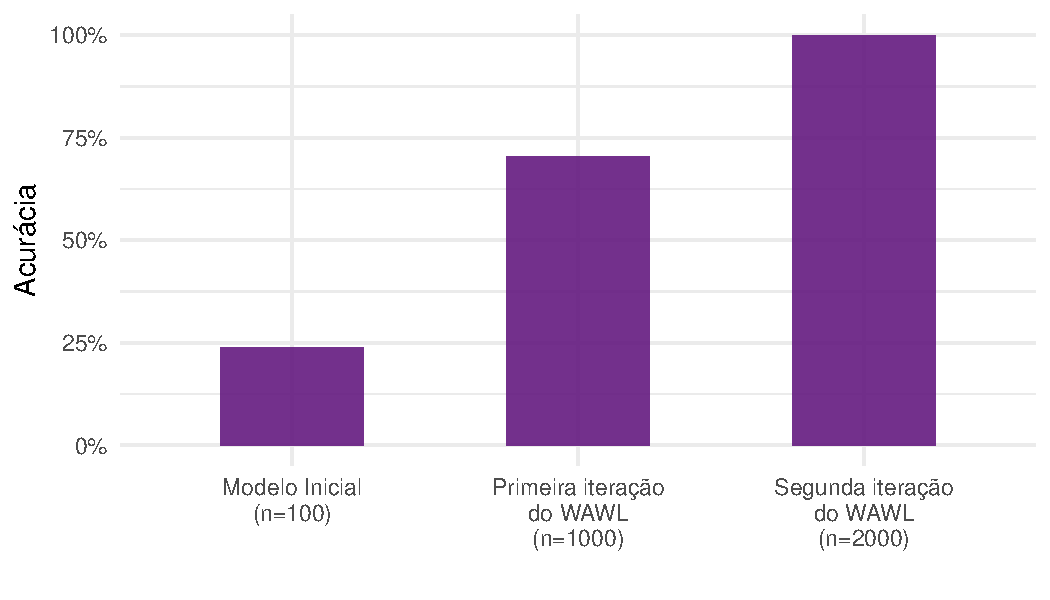
\includegraphics[width=0.85\textwidth,height=\textheight]{./resultados_files/figure-pdf/fig-aplicacao-iterada-1.pdf}

}

\caption{\label{fig-aplicacao-iterada}Resultados da aplicação iterada da
técnica.}

\end{figure}

O resultado sugere que a técnica pode ser utilizada em várias iterações
para auxiliar no aprendizado do modelo. Ela sugere, ainda, que uma
técnica de aprendizado ativo com \emph{feedback} automático do oráculo
pode dar bons resultados, já que a forma de obter os dados não introduz
viés de seleção no ajuste do modelo.

\hypertarget{sec-pacote-captcha}{%
\section{Pacote captcha}\label{sec-pacote-captcha}}

O pacote \texttt{\{captcha\}} foi construído para funcionar como uma
caixa de ferramentas para pessoas que desejam trabalhar com Captchas. O
pacote possui funções de leitura, visualização, anotação, preparação de
dados, modelagem, carregamento de modelos pré-treinados e predição. O
pacote também permite a construção de um fluxo de trabalho para resolver
um novo Captcha, criando um pacote para orquestrar o passo-a-passo.

\hypertarget{uso-buxe1sico}{%
\subsection{Uso básico}\label{uso-buxe1sico}}

A utilização básica do \texttt{\{captcha\}} envolve as funções
\texttt{read\_captcha()}, \texttt{plot()}, \texttt{captcha\_annotate()},
\texttt{captcha\_load\_model()} e \texttt{decrypt()}. As funções são
explicadas abaixo.

A função \texttt{read\_captcha()} lê um vetor de arquivos de imagens e
armazenar na memória. Por trás, a função utiliza o pacote
\texttt{\{magick\}} para lidar com os tipos de arquivos que podem
aparecer (JPEG, PNG, entre outros).

\begin{Shaded}
\begin{Highlighting}[]
\FunctionTok{library}\NormalTok{(captcha)}
\NormalTok{exemplo }\OtherTok{\textless{}{-}} \StringTok{"assets/img/dados\_tjmg.jpeg"}
\NormalTok{captcha }\OtherTok{\textless{}{-}} \FunctionTok{read\_captcha}\NormalTok{(exemplo)}

\NormalTok{captcha}
\CommentTok{\#\textgreater{} \# A tibble: 1 x 7}
\CommentTok{\#\textgreater{}   format width height colorspace matte filesize density}
\CommentTok{\#\textgreater{}   \textless{}chr\textgreater{}  \textless{}int\textgreater{}  \textless{}int\textgreater{} \textless{}chr\textgreater{}      \textless{}lgl\textgreater{}    \textless{}int\textgreater{} \textless{}chr\textgreater{}  }
\CommentTok{\#\textgreater{} 1 JPEG     100     50 sRGB       FALSE     4530 72x72}
\end{Highlighting}
\end{Shaded}

\begin{figure}[H]

{\centering 
\includegraphics[width=0.3\textwidth,height=\textheight]{./resultados_files/figure-pdf/fig-uso-basico-captcha-1.png}

}

\caption{\label{fig-uso-basico-captcha}\textbf{?(caption)}}

\end{figure}

A função retorna um objeto com a classe \texttt{captcha}, que pode ser
utilizada por outros métodos.

\begin{Shaded}
\begin{Highlighting}[]
\FunctionTok{class}\NormalTok{(captcha)}
\CommentTok{\#\textgreater{} [1] "captcha"}
\end{Highlighting}
\end{Shaded}

O objeto é uma lista com três elementos: \texttt{\$img}, que contém
imagem lida com o pacote \texttt{\{magick\}}, \texttt{\$lab}, que contém
o rótulo da imagem (por padrão, \texttt{NULL}) e \texttt{\$path}, que
contém o caminho da imagem que foi lida.

\begin{Shaded}
\begin{Highlighting}[]
\FunctionTok{str}\NormalTok{(captcha)}
\CommentTok{\#\textgreater{} Class \textquotesingle{}captcha\textquotesingle{}  hidden list of 3}
\CommentTok{\#\textgreater{}  $ img :Class \textquotesingle{}magick{-}image\textquotesingle{} \textless{}externalptr\textgreater{} }
\CommentTok{\#\textgreater{}  $ lab : NULL}
\CommentTok{\#\textgreater{}  $ path: chr "assets/img/dados\_tjmg.jpeg"}
\end{Highlighting}
\end{Shaded}

A função \texttt{read\_captcha()} possui um parâmetro
\texttt{lab\_in\_path=}, que indica se o rótulo está contido no caminho
da imagem. Se \texttt{lab\_in\_path=TRUE}, a função tentará extrair o
rótulo do arquivo (obtendo o texto que vem depois do último \texttt{\_}
do caminho) e armazenar no elemento \texttt{\$lab}.

\begin{Shaded}
\begin{Highlighting}[]
\NormalTok{exemplo }\OtherTok{\textless{}{-}} \StringTok{"assets/img/mnist128c49c36e13\_6297.png"}
\NormalTok{captcha }\OtherTok{\textless{}{-}} \FunctionTok{read\_captcha}\NormalTok{(exemplo, }\AttributeTok{lab\_in\_path =} \ConstantTok{TRUE}\NormalTok{)}

\FunctionTok{str}\NormalTok{(captcha)}
\CommentTok{\#\textgreater{} Class \textquotesingle{}captcha\textquotesingle{}  hidden list of 3}
\CommentTok{\#\textgreater{}  $ img :Class \textquotesingle{}magick{-}image\textquotesingle{} \textless{}externalptr\textgreater{} }
\CommentTok{\#\textgreater{}  $ lab : chr "6297"}
\CommentTok{\#\textgreater{}  $ path: chr "assets/img/mnist128c49c36e13\_6297.png"}
\end{Highlighting}
\end{Shaded}

A função plot \texttt{plot()} é um método de classe S3 do R básico. A
função foi implementada para facilitar a visualização de Captchas. A
função recebe uma lista de imagens obtida pela função
\texttt{read\_captcha()} e mostra o Captcha visualmente, como na
Figura~\ref{fig-exemplo-plot}.

\begin{Shaded}
\begin{Highlighting}[]
\NormalTok{exemplo }\OtherTok{\textless{}{-}} \StringTok{"assets/img/dados\_tjmg.jpeg"}
\NormalTok{captcha }\OtherTok{\textless{}{-}} \FunctionTok{read\_captcha}\NormalTok{(exemplo)}
\FunctionTok{plot}\NormalTok{(captcha)}
\end{Highlighting}
\end{Shaded}

\begin{figure}[H]

{\centering 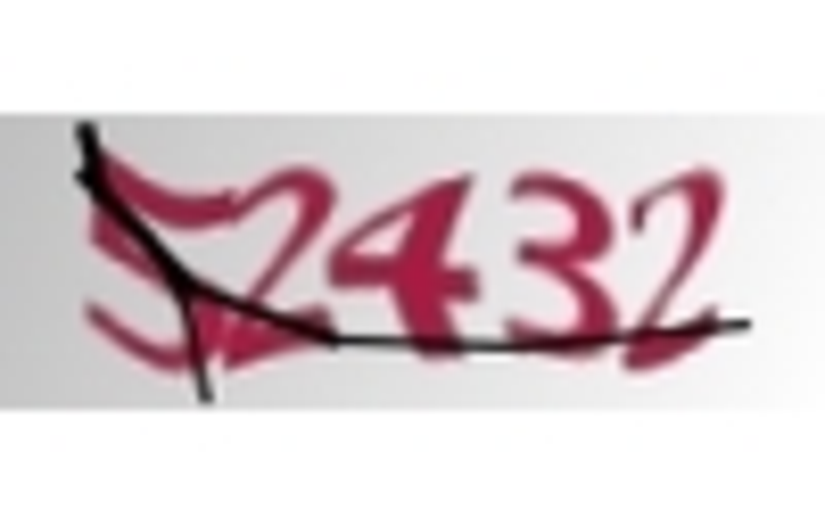
\includegraphics[width=0.3\textwidth,height=\textheight]{./resultados_files/figure-pdf/fig-exemplo-plot-1.pdf}

}

\caption{\label{fig-exemplo-plot}Exemplo de aplicação da função plot a
um objeto \texttt{captcha}.}

\end{figure}

Um aspecto interessante da função \texttt{plot()} é que ela lida com uma
lista de Captchas. Isso é útil quando o interesse é visualizar vários
Captchas de uma vez na imagem. A Figura~\ref{fig-exemplo-plot-multi}
mostra um exemplo de aplicação.

\begin{Shaded}
\begin{Highlighting}[]
\NormalTok{exemplos }\OtherTok{\textless{}{-}} \FunctionTok{paste0}\NormalTok{(}\StringTok{"assets/img/"}\NormalTok{, }\FunctionTok{c}\NormalTok{(}
  \StringTok{"dados\_tjmg.jpeg"}\NormalTok{,}
  \StringTok{"dados\_esaj.png"}\NormalTok{,}
  \StringTok{"dados\_rfb.png"}\NormalTok{,}
  \StringTok{"dados\_sei.png"}
\NormalTok{))}
\NormalTok{captchas }\OtherTok{\textless{}{-}} \FunctionTok{read\_captcha}\NormalTok{(exemplos)}
\FunctionTok{plot}\NormalTok{(captchas)}
\end{Highlighting}
\end{Shaded}

\begin{figure}[H]

{\centering 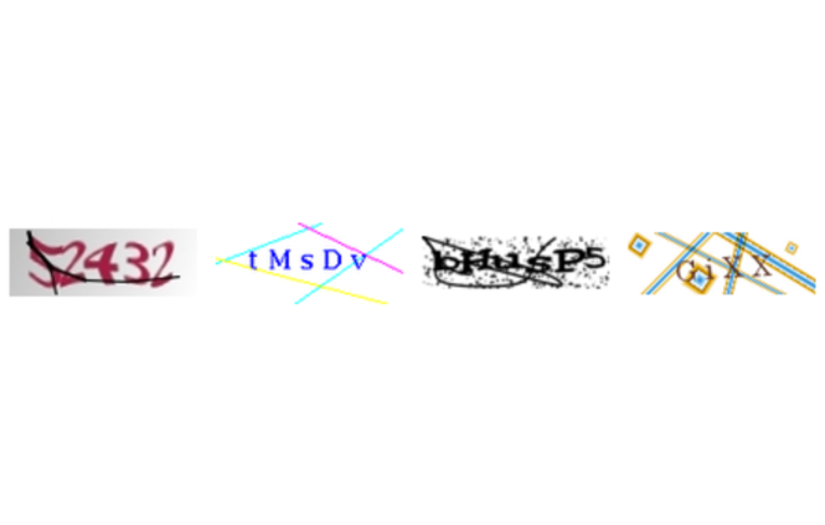
\includegraphics[width=0.7\textwidth,height=\textheight]{./resultados_files/figure-pdf/fig-exemplo-plot-multi-1.pdf}

}

\caption{\label{fig-exemplo-plot-multi}Exemplo de aplicação da função
plot a um objeto \texttt{captcha} com várias imagens.}

\end{figure}

Por padrão, a função plot dispõe as imagens em quatro colunas. Para
mudar o padrão, é possível modificar as opções usando
\texttt{options(captcha.print.cols\ =\ N)}, onde \texttt{N} é o número
de colunas desejado. A Figura~\ref{fig-exemplo-plot-multi-2col} mostra
um exemplo com duas colunas.

\begin{Shaded}
\begin{Highlighting}[]
\FunctionTok{options}\NormalTok{(}\AttributeTok{captcha.print.cols =} \DecValTok{2}\NormalTok{)}
\FunctionTok{plot}\NormalTok{(captchas)}
\end{Highlighting}
\end{Shaded}

\begin{figure}[H]

{\centering 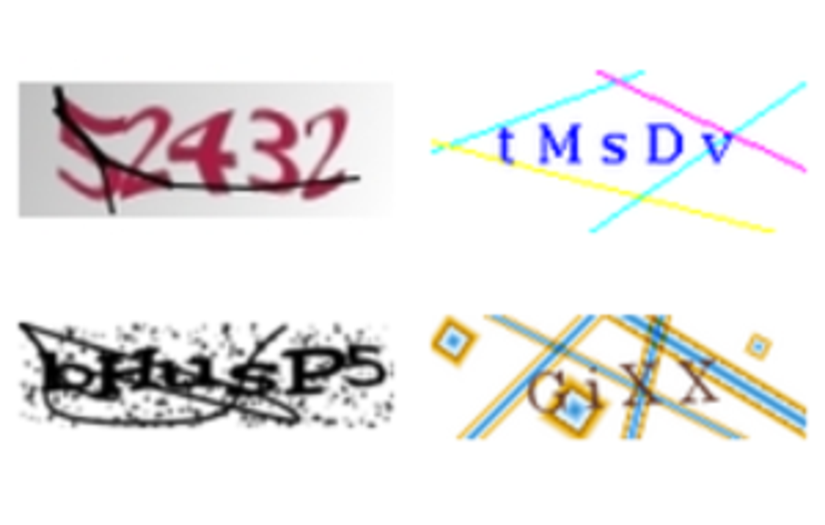
\includegraphics[width=0.6\textwidth,height=\textheight]{./resultados_files/figure-pdf/fig-exemplo-plot-multi-2col-1.pdf}

}

\caption{\label{fig-exemplo-plot-multi-2col}Exemplo de aplicação da
função plot a um objeto \texttt{captcha} com várias imagens,
disponibilizadas em duas colunas.}

\end{figure}

Quando o vetor de Captchas é muito grande, a função \texttt{plot()}
mostra um número máximo de 100 imagens, acompanhado de uma mensagem. O
padrão de 100 imagens está organizado em uma grade com 25 linhas e 4
colunas, podendo ser sobrescrito ao combinar as opções
\texttt{captcha.print.cols=} e \texttt{captcha.print.rows=}. A
Figura~\ref{fig-exemplo-plot-multi-varias} mostra um exemplo do
comportamento da função quando o número de imagens excede 100.

\begin{Shaded}
\begin{Highlighting}[]
\CommentTok{\# mais de 100 imagens:}
\NormalTok{exemplos }\OtherTok{\textless{}{-}} \FunctionTok{rep}\NormalTok{(}\StringTok{"assets/img/dados\_tjmg.jpeg"}\NormalTok{, }\DecValTok{110}\NormalTok{)}
\NormalTok{captchas }\OtherTok{\textless{}{-}} \FunctionTok{read\_captcha}\NormalTok{(exemplos)}
\FunctionTok{plot}\NormalTok{(captchas)}
\CommentTok{\#\textgreater{} i Too many images, printing first 100. To override, run}
\CommentTok{\#\textgreater{} * options(\textquotesingle{}captcha.print.rows\textquotesingle{} = MAX\_ROWS)}
\CommentTok{\#\textgreater{} * options(\textquotesingle{}captcha.print.cols\textquotesingle{} = COLUMNS)}
\end{Highlighting}
\end{Shaded}

\begin{figure}[H]

{\centering 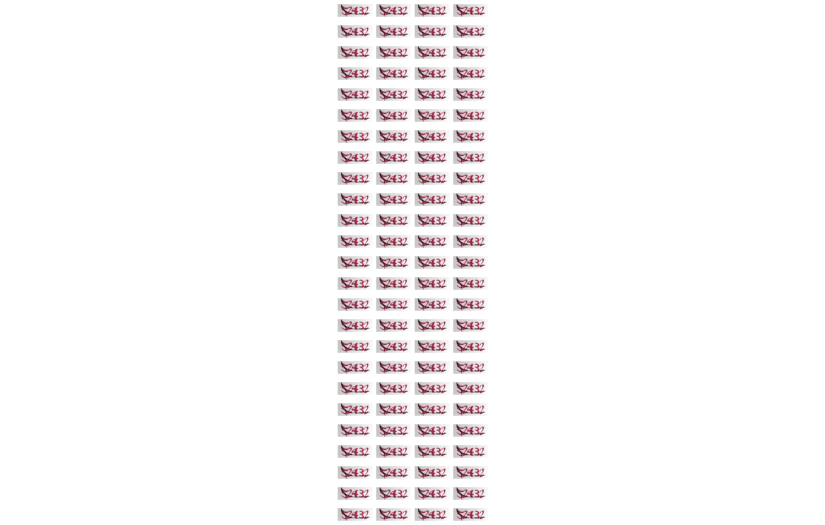
\includegraphics{./resultados_files/figure-pdf/fig-exemplo-plot-multi-varias-1.pdf}

}

\caption{\label{fig-exemplo-plot-multi-varias}Demonstração da função
\texttt{plot()} com muitas imagens.}

\end{figure}

Um detalhe interessante é que é possível criar subconjuntos de um objeto
de classe \texttt{captcha} simplesmente utilizando o operador
\texttt{{[}}. A função \texttt{length()} também pode ser utilizada para
medir a quantidade de imagens lidas. A
Figura~\ref{fig-exemplo-plot-multi-varias-subset} mostra um exemplo
dessas operações.

\begin{Shaded}
\begin{Highlighting}[]
\NormalTok{captchas\_subset }\OtherTok{\textless{}{-}}\NormalTok{ captchas[}\DecValTok{1}\SpecialCharTok{:}\DecValTok{20}\NormalTok{]}
\FunctionTok{length}\NormalTok{(captchas\_subset) }\CommentTok{\# 20}
\CommentTok{\#\textgreater{} [1] 20}
\FunctionTok{plot}\NormalTok{(captchas\_subset)}
\end{Highlighting}
\end{Shaded}

\begin{figure}[H]

{\centering 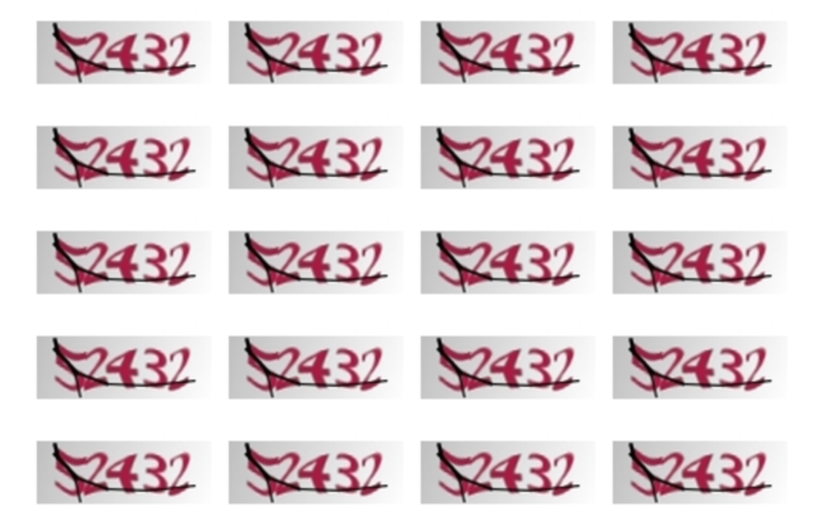
\includegraphics{./resultados_files/figure-pdf/fig-exemplo-plot-multi-varias-subset-1.pdf}

}

\caption{\label{fig-exemplo-plot-multi-varias-subset}Demonstração das
funções de subset e length aplicadas a um objeto do tipo
\texttt{captcha}.}

\end{figure}

Por fim, se a imagem possui um rótulo, por padrão, a função
\texttt{plot()} mostra o rótulo no canto da imagem. A
Figura~\ref{fig-exemplo-plot-rotulado} mostra um exemplo.

\begin{Shaded}
\begin{Highlighting}[]
\NormalTok{exemplo }\OtherTok{\textless{}{-}} \StringTok{"assets/img/mnist128c49c36e13\_6297.png"}
\NormalTok{captcha }\OtherTok{\textless{}{-}} \FunctionTok{read\_captcha}\NormalTok{(exemplo, }\AttributeTok{lab\_in\_path =} \ConstantTok{TRUE}\NormalTok{)}
\FunctionTok{plot}\NormalTok{(captcha)}
\end{Highlighting}
\end{Shaded}

\begin{figure}[H]

{\centering 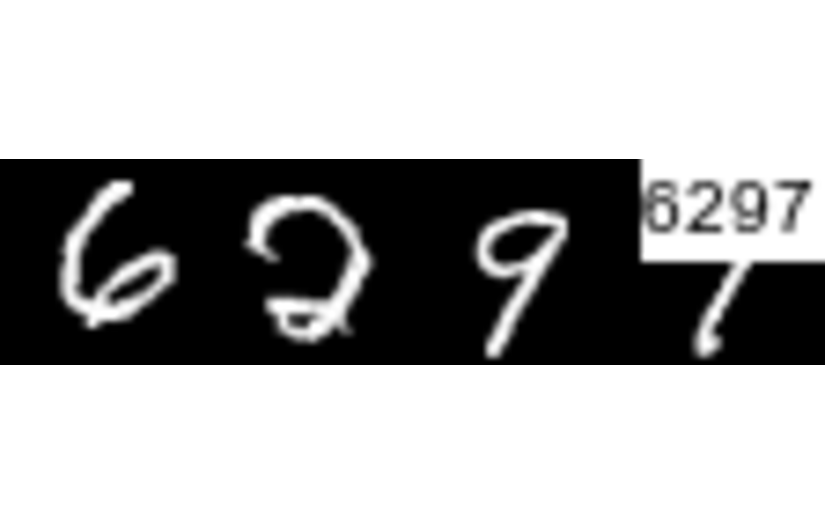
\includegraphics[width=0.3\textwidth,height=\textheight]{./resultados_files/figure-pdf/fig-exemplo-plot-rotulado-1.pdf}

}

\caption{\label{fig-exemplo-plot-rotulado}Demonstração da função
\texttt{plot()} quando o Captcha possui um rótulo}

\end{figure}

A função \texttt{captcha\_annotate()} serve para anotar o rótulo de uma
imagem de Captcha, manual ou automaticamente. Isso é feito modificando o
caminho da imagem, adicionando o texto \texttt{\_rotulo} ao final do
caminho do arquivo. A função possui os parâmetros listados abaixo:

\begin{itemize}
\tightlist
\item
  \texttt{files=}: objeto de classe \texttt{captcha} lido com a função
  \texttt{read\_captcha()} (recomendado) ou vetor de caminhos de
  arquivos.
\item
  \texttt{labels=}: (opcional) vetor com os rótulos das imagens. Deve
  ter o mesmo \texttt{length()} do que \texttt{files=}. Por padrão, o
  valor é \texttt{NULL}, indicando que deve ser aberto um
  \texttt{prompt} para que o usuário insira a resposta manualmente.
\item
  \texttt{path=}: (opcional) caminho da pasta onde os arquivos anotados
  serão salvos. Por padrão, salva os arquivos com nomes modificados na
  mesma pasta dos arquivos originais.
\item
  \texttt{rm\_old=}: (opcional) deletar ou não os arquivos originais.
  Por padrão, é \texttt{FALSE}.
\end{itemize}

A função, depois de aplicada, retorna um vetor com os caminhos dos
arquivos modificados. O parâmetro \texttt{labels=} é útil para lidar com
situações em que sabemos o rótulo do Captcha. Por exemplo, em um fluxo
de trabalho que utiliza o oráculo, pode ser que um modelo inicial já
forneça o valor correto do rótulo.

Quando não existe um rótulo, a função \texttt{captcha\_annotate()}, que
abre o \texttt{prompt} para anotação e aplica \texttt{plot()} para
visualizar a imagem. A Figura~\ref{fig-exemplo-annotate} mostra um
exemplo de aplicação da função \texttt{captcha\_annotate()} no software
\href{https://posit.co/download/rstudio-desktop/}{RStudio}.

\begin{figure}

{\centering \includegraphics{./assets/img/exemplo_annotate.png}

}

\caption{\label{fig-exemplo-annotate}Exemplo de aplicação da função
\texttt{captcha\_annotate()}. O rótulo \texttt{bhusp5} foi inserido
manualmente.}

\end{figure}

Por último, a função \texttt{decrypt()} tem o papel de obter o rótulo de
uma imagem utilizando um modelo já treinado para aquele tipo de imagem.
A função recebe dois argumentos: \texttt{file=} que pode ser tanto o
caminho do arquivo quanto um objeto de classe \texttt{captcha}, e um
argumento \texttt{model=}, que contém um modelo de classe
\texttt{luz\_module\_fitted}, ajustado utilizando as ferramentas que
serão apresentadas na próxima subseção.

Para a tese, foram desenvolvidos modelos para vários Captchas
diferentes. É possível carregar um modelo já treinado usando a função
\texttt{captcha\_load\_model()}, podendo receber em seu único parâmetro
\texttt{path=} o caminho de um arquivo contendo um modelo ajustado ou
uma \emph{string} com o nome de um modelo já treinado, como
\texttt{"rfb"}, por exemplo. Os modelos treinados são armazenados nos
\href{https://github.com/decryptr/captcha/releases}{releases do
repositório do pacote captcha}, são baixados e controlados pelo pacote
\texttt{\{piggyback\}} (BOETTIGER; HO, 2022) e são lidos utilizando o
pacote \texttt{\{luz\}}, que será descrito em maiores detalhes na
próxima subseção. No momento de submissão da tese, os Captchas com
modelos desenvolvidos eram \texttt{trf5}, \texttt{tjmg}, \texttt{trt},
\texttt{esaj}, \texttt{jucesp}, \texttt{tjpe}, \texttt{tjrs},
\texttt{cadesp}, \texttt{sei} e \texttt{rfb}.

A Figura~\ref{fig-diagrama-captcha-simples} resume visualmente as
funções apresentadas até o momento. As setas indicam a dependência das
funções de objetos gerados por outras funções.

\begin{figure}

{\centering 

\begin{figure}[H]

{\centering 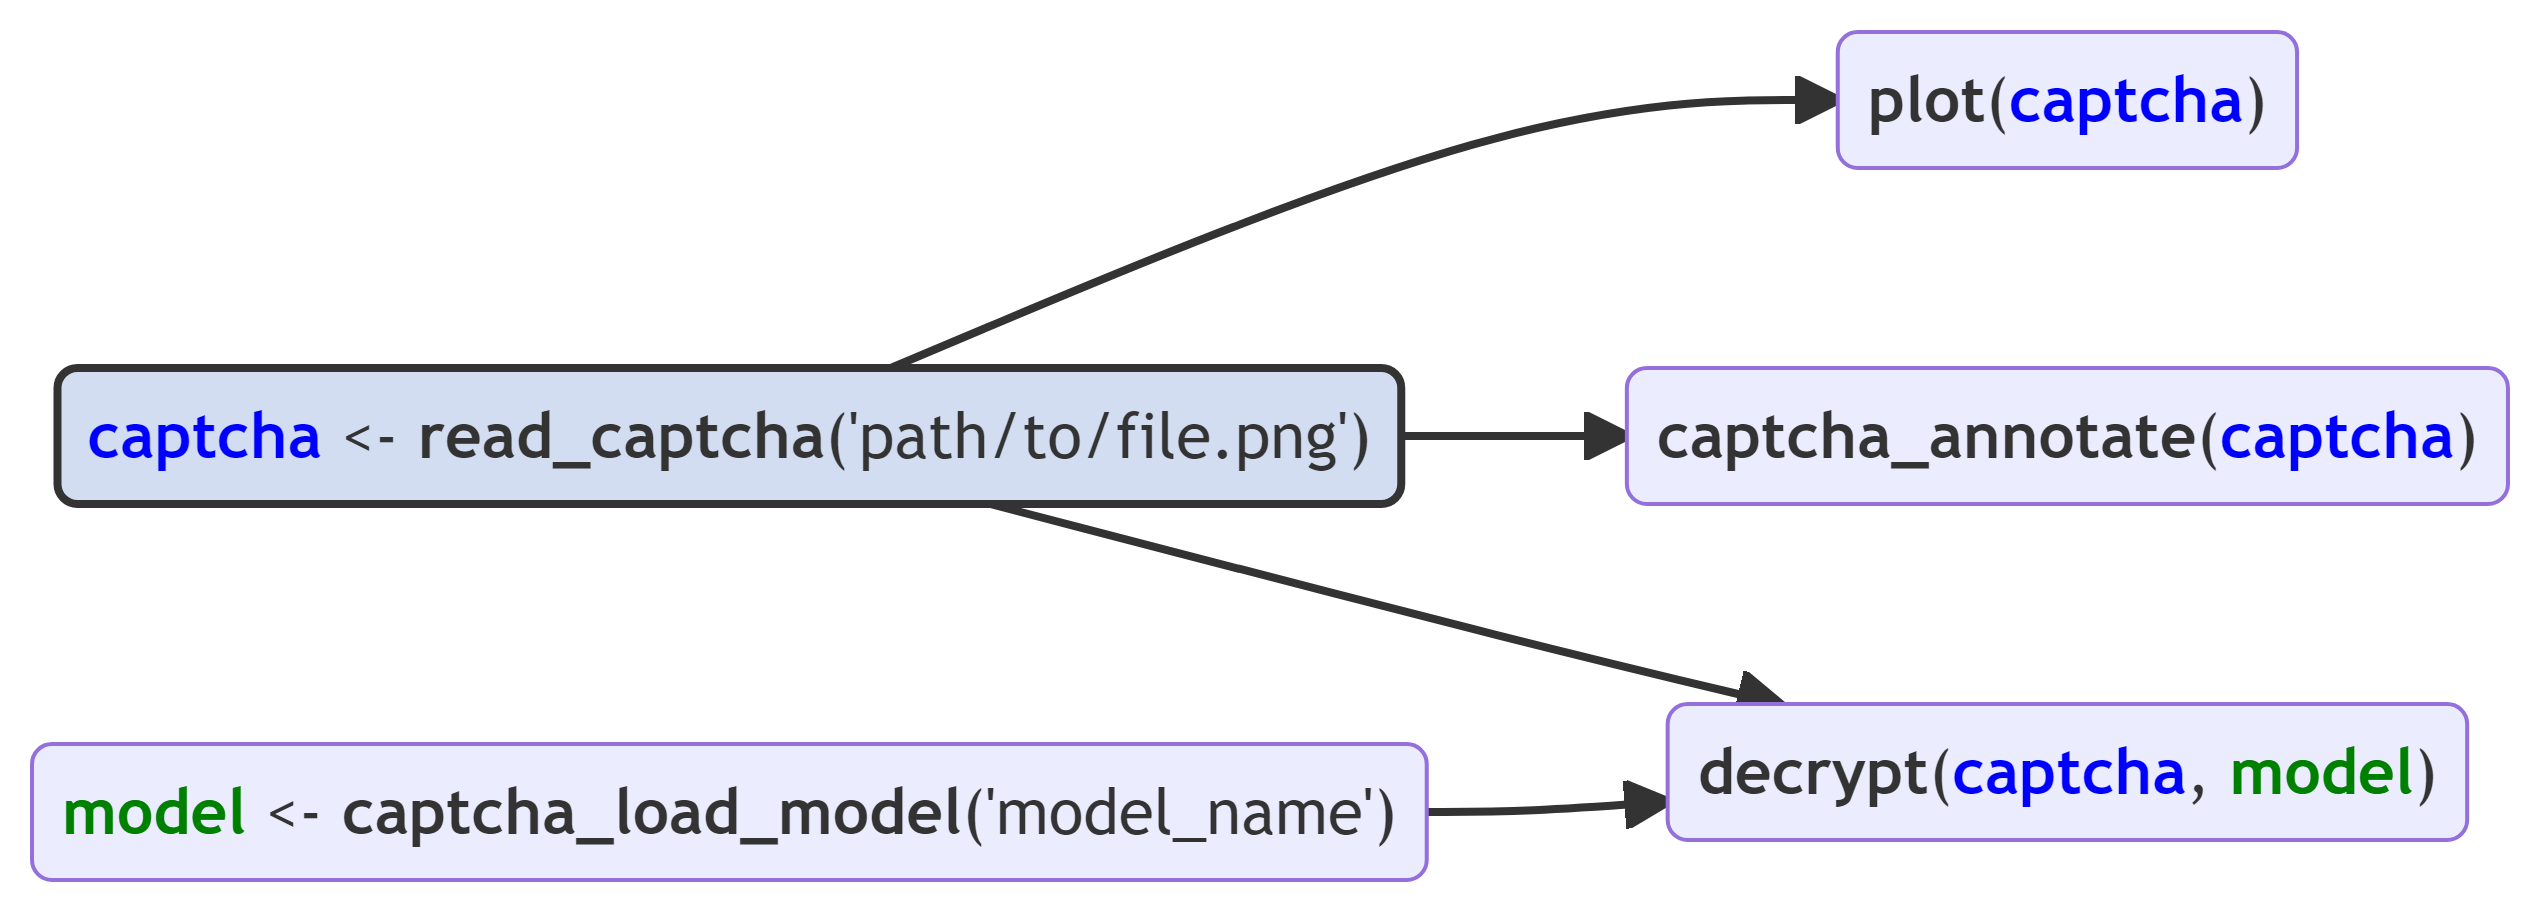
\includegraphics[width=6.61in,height=2.38in]{./resultados_files/figure-latex/mermaid-figure-1.png}

}

\end{figure}

}

\caption{\label{fig-diagrama-captcha-simples}Diagrama das funções
básicas do pacote \texttt{\{captcha\}}}

\end{figure}

\hypertarget{sec-ap-modelagem}{%
\subsection{Modelagem}\label{sec-ap-modelagem}}

O pacote \texttt{\{captcha\}} também fornece uma interface básica para o
desenvolvimento de modelos a partir de uma base completamente anotada. A
anotação pode ser feita manualmente pela função
\texttt{captcha\_annotate()}, apresentada anteriormente, ou por outro
método desenvolvido pelo usuário.

A parte de modelagem parte de algumas premissas sobre a base de dados.
As imagens precisam estar em uma pasta e ter o padrão
\texttt{caminho/do/arquivo/\textless{}id\textgreater{}\_\textless{}lab\textgreater{}.\textless{}ext\textgreater{}},
onde:

\begin{itemize}
\tightlist
\item
  \texttt{\textless{}id\textgreater{}}: pode ser qualquer nome, de
  preferência sem acentuação ou outros caracteres especiais, para evitar
  problemas de \emph{encoding}. Geralmente, é um \emph{hash}
  identificando o tipo e id do captcha. \textbf{Nota}: ao anotar um
  caso, é importante que o \texttt{id} seja único, já que dois Captchas
  podem ter o mesmo rótulo.
\item
  \texttt{\textless{}lab\textgreater{}}: é o rótulo do Captcha. Pode ser
  um conjunto de caracteres entre \texttt{{[}a-zA-Z0-9{]}},
  diferenciando maiúsculas e minúsculas se necessário. No momento, todos
  os arquivos em uma pasta devem ter a mesma quantidade de caracteres
  (comprimento homogêneo). Futuramente, o pacote poderá considerar
  Captchas de comprimento heterogêneo.
\item
  \texttt{\textless{}ext\textgreater{}}: extensão do arquivo. Pode ser
  \texttt{.png}, \texttt{.jpeg} ou \texttt{.jpg}. As operações também
  funcionam para o formato \texttt{.svg}, mas pode apresentar problemas
  por conta da transparência da imagem.
\end{itemize}

Atendidas as premissas da base anotada, é possível ajustar um modelo de
redes neurais usando o pacote \texttt{\{captcha\}}. No entanto, como o
ajuste de modelos de redes neurais envolve uma série de nuances e
pequenas adaptações, optou-se por exportar funções em dois níveis de
aprofundamento. A primeira é a \textbf{automatizada}, utilizando a
função \texttt{captcha\_fit\_model()} descrito a seguir, enquanto a
segunda é a \textbf{procedimental}, utilizando o passo a passo descrito
na Subseção \ref{sec-captcha-do-zero}.

A função \texttt{captcha\_fit\_model()} ajusta um modelo a partir de uma
pasta com arquivos anotados. A função recebe os parâmetros:
\texttt{dir=}, contendo o caminho dos arquivos anotados;
\texttt{dir\_valid=}, (opcional) contendo o caminho dos arquivos
anotados para validação; \texttt{prop\_valid=}, contendo a proporção da
base de treino a ser considerada como validação, ignorada quando
\texttt{dir\_valid=} é fornecida (por padrão, considera-se 20\% da base
para validação).

A função \texttt{captcha\_fit\_model()} também possui alguns parâmetros
relacionados à modelagem. São eles: \texttt{dropout=}, especificando o
percentual de \emph{dropout} aplicado às camadas ocultas da rede (por
padrão, \texttt{0.25}); \texttt{dense\_units=}, especificando a
quantidade de unidades na camada oculta que vem depois das camadas
convolucionais (por padrão, 200); \texttt{decay=}, especificando o
percentual de decaimento da taxa de aprendizado (por padrão,
\texttt{0.99}); \texttt{epochs=} número de épocas para ajuste do modelo
(por padrão 100). Uma observação importante é que o modelo está
configurado para parar o ajuste após 20 iterações sem redução
significativa na função de perda (arbitrado em 1\%; para mais detalhes
ver a Subseção \ref{sec-captcha-do-zero}).

No final, a função retorna um modelo ajustado com classe
\texttt{luz\_module\_fitted}, que pode ser salvo em disco utilizando-se
a função \texttt{luz\_save()}. O modelo também pode ser serializado para
utilização em outros pacotes como pytorch. Um tutorial sobre
serialização pode ser encontrado na
\href{https://torch.mlverse.org/docs/articles/serialization.html}{documentação
do pacote torch}.

O pacote \texttt{\{captchaOracle\}} possui uma interface similar para
trabalhar com bases com rótulos parciais. Como a estrutura de dados
nesse caso é mais complexa e pode evoluir no futuro, os códigos foram
organizados em outro pacote. Mais detalhes na Seção
\ref{sec-pacote-oracle}.

Na documentação do pacote \texttt{\{captcha\}}, foi adicionado um
exemplo de aplicação. O exemplo utiliza captchas gerados usando a função
\texttt{captcha\_generate()}, que gera Captchas utilizando o pacote
\texttt{\{magick\}}. O Captcha foi criado para a construção da tese,
apelidado de \texttt{R-Captcha}, e possui os seguintes parâmetros:

\begin{itemize}
\tightlist
\item
  \texttt{write\_disk=}: salvar os arquivos em disco? Por padrão, é
  falso.
\item
  \texttt{path=}: Caminho para salvar arquivos em disco, caso o
  parâmetro anterior seja verdadeiro.
\item
  \texttt{chars=}: Quais caracteres usar na imagem.
\item
  \texttt{n\_chars=}: O comprimento do Captcha.
\item
  \texttt{n\_rows=}: Altura da imagem, em pixels.
\item
  \texttt{n\_cols=}: Largura da imagem, em pixels.
\item
  \texttt{p\_rotate=}: Probabilidade de rotação da imagem.
\item
  \texttt{p\_line=}: Probabilidade de adicionar um risco entre as
  letras.
\item
  \texttt{p\_stroke=}: Probabilidade de adicionar uma borda nas letras.
\item
  \texttt{p\_box=}: Probabilidade de adicionar uma caixa (retângulo) em
  torno das letras.
\item
  \texttt{p\_implode=}: Probabilidade de adicionar efeitos de implosão.
\item
  \texttt{p\_oilpaint=}: Probabilidade de adicionar efeitos de tinta a
  óleo.
\item
  \texttt{p\_noise=}: Probabilidade de adicionar um ruído branco no
  fundo da imagem.
\item
  \texttt{p\_lat=}: Probabilidade de aplicar o algoritmo \emph{local
  adaptive thresholding} à imagem.
\end{itemize}

\hypertarget{sec-captcha-do-zero}{%
\subsection{Resolvendo um novo Captcha do
zero}\label{sec-captcha-do-zero}}

Em algumas situações, pode ser desejável rodar modelos de forma
customizada. Isso acontece pois modelos de aprendizagem profunda
costumam precisar de diversos pequenos ajustes, como a taxa de
aprendizado, utilização de outras funções de otimização, camadas
computacionais e funções de pré-processamento.

A função \texttt{captcha\_fit\_model()}, apresentada na subseção
anterior, é engessada. Ela aceita alguns parâmetros para estruturar o
modelo, mas não possui elementos suficientes para customização. É para
isso que pacotes como \texttt{\{torch\}} e \texttt{\{luz\}} existem,
pois criam ambientes de computação mais flexíveis para operar os modelos
de aprendizado profundo.

Outra desvantagem da utilização do \texttt{captcha\_fit\_model()} é a
disponibilização dos modelos. Um modelo pode ser utilizado localmente,
mas a tarefa de disponibilizar as bases de dados e o modelo para outras
pessoas não tem um procedimento bem definido.

Para organizar o fluxo de trabalho, implementou-se um fluxo de anotação
de Captchas dentro do pacote \texttt{\{captcha\}}. A função que
orquestra esse fluxo é a \texttt{new\_captcha()}. A função possui apenas
um parâmetro, \texttt{path=}, que é o caminho de uma nova pasta a ser
criada.

A função também pode ser chamada criando-se um projeto dentro do próprio
RStudio. A Figura~\ref{fig-exemplo-rstudio-template} mostra um exemplo
de utilização do template dentro do RStudio, após clicar em
\texttt{Novo\ Projeto\ \textgreater{}\ Novo\ Diretório}.

\begin{figure}

{\centering \includegraphics{./assets/img/exemplo-rstudio-template.png}

}

\caption{\label{fig-exemplo-rstudio-template}Exemplo de criação de um
novo projeto de Captcha utilizando o RStudio.}

\end{figure}

Ao criar um novo projeto, pelo comando \texttt{new\_captcha()} ou pela
interface do RStudio, uma nova janela é aberta. O projeto contém quatro
arquivos:

\begin{itemize}
\tightlist
\item
  \texttt{01\_download.R}: Contém algumas funções para auxiliar no
  desenvolvimento de funções que baixam Captchas em um caso real. Na
  prática, as funções que baixam Captchas precisam ser adaptadas porque
  os sites são organizados de formas muito diferentes.
\item
  \texttt{02\_annotate.R}: Contém um \emph{template} para anotação
  manual de Captchas. A anotação manual pode tanto ser realizada usando
  a interface criada pelo pacote \texttt{\{captcha\}} quanto
  externamente. No final, os arquivos anotados devem ser salvos na pasta
  \texttt{img}, no formato descrito na Subseção \ref{sec-ap-modelagem}.
\item
  \texttt{03\_model.R}: Contém um \emph{template} para modelagem,
  permitindo a customização completa do procedimento de ajuste. O
  \emph{script} contém comandos para carregar os dados, especificar o
  modelo, realizar o ajuste e salvar o modelo ajustado.
\item
  \texttt{04\_share.R}: Contém funções para criar um repositório
  \emph{git} da solução e disponibilizar o modelo ajustado. O modelo
  poderá ser lido e aplicado utilizando-se a função
  \texttt{captcha\_load\_model()}, para utilização em diferentes
  contextos, sem a necessidade de copiar arquivos localmente.
\end{itemize}

Sobre a parte de modelagem, cabe uma descrição mais detalhada. O
primeiro passo do \emph{script} é criar objetos do tipo \emph{dataset}
(objeto que armazena os dados de forma consistente) e \emph{dataloader}
(objeto que obtém amostras do dataset, que são utilizadas como os
\emph{minibatches} do modelo), com uma estrutura orquestrada pelo pacote
\texttt{\{torch\}}.

A função \texttt{captcha\_dataset()} cria o \emph{dataset}, recebendo
como parâmetro uma pasta de arquivos e gera um objeto com classes
\texttt{my\_captcha}, \texttt{dataset} e \texttt{R6}. A função é, na
verdade, um objeto do tipo \texttt{dataset\_generator}, criada
utilizando a função \texttt{dataset()} do pacote \texttt{\{torch\}}. O
objeto é chamado da mesma forma que uma função usual do R, aceitando
alguns parâmetros adicionais:

\begin{itemize}
\tightlist
\item
  \texttt{transform\_image=}: operação de transformação a ser aplicada à
  imagem. Por padrão, utiliza a função
  \texttt{captcha\_transform\_image()}, que lê a imagem e redimensiona
  para ficar com dimensões \texttt{32x192}. A dimensão foi escolhida
  para facilitar a implementação das camadas convolucionais e para lidar
  com o fato de que usualmente os Captchas são imagens retangulares.
\item
  \texttt{transform\_label=}: operação de transformação para gerar a
  variável resposta. Por padrão, utiliza a função
  \texttt{captcha\_transform\_label()}, que recebe um vetor de todos os
  possíveis caracteres do Captcha e aplica a operação
  \texttt{one\_hot()}, obtendo-se a versão matricial da resposta com
  zeros e uns, como descrito na Seção~\ref{sec-definicao-captcha}.
\item
  \texttt{augmentation=}: operações para aumentação de dados. Por
  exemplo, pode ser uma função que adiciona um ruído aleatório à imagem
  original para que, ao gerar uma nova amostra, os dados utilizados
  sejam sempre diferentes.
\end{itemize}

A função \texttt{captcha\_dataset()} deve ser aplicada duas vezes, uma
para criar a base de treino e outra para criar a base de validação. A
separação de bases de treino e validação deve ser feita de forma manual,
copiando parte dos Captchas anotados para uma nova pasta, com
aleatorização. É papel do usuário separar as bases em pastas distintas
carregá-as em um \emph{dataset}.

Em seguida, os \emph{dataloaders} são criados utilizando-se a função
\texttt{dataloader()} do pacote \texttt{\{torch\}}. Nessa parte é
definido o tamanho do \emph{minibatch}, além de outros possíveis
parâmetros disponíveis na função do \texttt{\{torch\}}. Para mais
detalhes, o usuário pode
\href{https://torch.mlverse.org/docs/reference/dataloader.html}{acessar
a documentação da função neste link}. Devem ser criados
\emph{dataloaders} tanto para a base de treino quanto para a base de
validação.

A próxima etapa é a especificação do modelo. No \emph{script} de
modelagem, o modelo é fornecido pelo objeto \texttt{net\_captcha} do
pacote \texttt{\{captcha\}}. Assim como no caso do \emph{dataset}, o
\texttt{net\_captcha} é um objeto especial do \texttt{\{torch\}}, com
classes \texttt{CAPTCHA-CNN}, \texttt{nn\_module} e
\texttt{nn\_module\_generator}. O objeto pode ser utilizado como uma
função, gerando um módulo do \texttt{torch}, similar a uma função de
predição. No entanto, por conta da forma que o objeto é utilizado em
passos posteriores pelo pacote \texttt{\{luz\}}, o objeto a ser
considerado é mesmo o \texttt{nn\_module\_generator}, como colocado no
\emph{script}.

Para customizar o modelo, o usuário deve modificar os métodos
\texttt{initialize()} e \texttt{forward()}, acessados dentro do objeto
\texttt{net\_captcha\$public\_methods}. O primeiro é responsável pela
inicialização do modelo, contendo a descrição das operações que são
realizadas, como convoluções. O segundo é a função \emph{feed forward}
das redes neurais, que recebe uma imagem e retorna um objeto contendo os
\emph{logitos} ou probabilidades, no formato da variável resposta.

Por padrão, o código de inicialização do modelo é o descrito abaixo. Os
parâmetros \texttt{input\_dim=}, \texttt{output\_ndigits=},
\texttt{output\_vocab\_size=} e \texttt{vocab=} descrevem,
respectivamente, as dimensões da imagem, o comprimeiro da resposta, o
comprimento do alfabeto e os elementos do alfabeto. Os parâmetros
\texttt{transform=}, \texttt{dropout=} e \texttt{dense\_units=}
controlam, respectivamente, a função de transformação da imagem, os
hiperparâmetros de \emph{dropout} e a quantidade de unidades na camada
densa. É possível notar que os parâmetros das convoluções são fixos, já
preparados para funcionar bem com uma imagem de dimensões
\texttt{32x192}.

\begin{Shaded}
\begin{Highlighting}[]
\NormalTok{initialize }\OtherTok{=} \ControlFlowTok{function}\NormalTok{(input\_dim,}
\NormalTok{                      output\_ndigits,}
\NormalTok{                      output\_vocab\_size,}
\NormalTok{                      vocab,}
\NormalTok{                      transform,}
                      \AttributeTok{dropout =} \FunctionTok{c}\NormalTok{(.}\DecValTok{25}\NormalTok{, .}\DecValTok{25}\NormalTok{),}
                      \AttributeTok{dense\_units =} \DecValTok{400}\NormalTok{) \{}
  
  \CommentTok{\# in\_channels, out\_channels, kernel\_size, stride = 1, padding = 0}
\NormalTok{  self}\SpecialCharTok{$}\NormalTok{batchnorm0 }\OtherTok{\textless{}{-}}\NormalTok{ torch}\SpecialCharTok{::}\FunctionTok{nn\_batch\_norm2d}\NormalTok{(}\DecValTok{3}\NormalTok{)}
\NormalTok{  self}\SpecialCharTok{$}\NormalTok{conv1 }\OtherTok{\textless{}{-}}\NormalTok{ torch}\SpecialCharTok{::}\FunctionTok{nn\_conv2d}\NormalTok{(}\DecValTok{3}\NormalTok{, }\DecValTok{32}\NormalTok{, }\DecValTok{3}\NormalTok{)}
\NormalTok{  self}\SpecialCharTok{$}\NormalTok{batchnorm1 }\OtherTok{\textless{}{-}}\NormalTok{ torch}\SpecialCharTok{::}\FunctionTok{nn\_batch\_norm2d}\NormalTok{(}\DecValTok{32}\NormalTok{)}
\NormalTok{  self}\SpecialCharTok{$}\NormalTok{conv2 }\OtherTok{\textless{}{-}}\NormalTok{ torch}\SpecialCharTok{::}\FunctionTok{nn\_conv2d}\NormalTok{(}\DecValTok{32}\NormalTok{, }\DecValTok{64}\NormalTok{, }\DecValTok{3}\NormalTok{)}
\NormalTok{  self}\SpecialCharTok{$}\NormalTok{batchnorm2 }\OtherTok{\textless{}{-}}\NormalTok{ torch}\SpecialCharTok{::}\FunctionTok{nn\_batch\_norm2d}\NormalTok{(}\DecValTok{64}\NormalTok{)}
\NormalTok{  self}\SpecialCharTok{$}\NormalTok{conv3 }\OtherTok{\textless{}{-}}\NormalTok{ torch}\SpecialCharTok{::}\FunctionTok{nn\_conv2d}\NormalTok{(}\DecValTok{64}\NormalTok{, }\DecValTok{64}\NormalTok{, }\DecValTok{3}\NormalTok{)}
\NormalTok{  self}\SpecialCharTok{$}\NormalTok{batchnorm3 }\OtherTok{\textless{}{-}}\NormalTok{ torch}\SpecialCharTok{::}\FunctionTok{nn\_batch\_norm2d}\NormalTok{(}\DecValTok{64}\NormalTok{)}
\NormalTok{  self}\SpecialCharTok{$}\NormalTok{dropout1 }\OtherTok{\textless{}{-}}\NormalTok{ torch}\SpecialCharTok{::}\FunctionTok{nn\_dropout2d}\NormalTok{(dropout[}\DecValTok{1}\NormalTok{])}
\NormalTok{  self}\SpecialCharTok{$}\NormalTok{dropout2 }\OtherTok{\textless{}{-}}\NormalTok{ torch}\SpecialCharTok{::}\FunctionTok{nn\_dropout2d}\NormalTok{(dropout[}\DecValTok{2}\NormalTok{])}
  
\NormalTok{  self}\SpecialCharTok{$}\NormalTok{fc1 }\OtherTok{\textless{}{-}}\NormalTok{ torch}\SpecialCharTok{::}\FunctionTok{nn\_linear}\NormalTok{(}
    \CommentTok{\# must be the same as last convnet}
    \AttributeTok{in\_features =} \FunctionTok{prod}\NormalTok{(}\FunctionTok{calc\_dim\_conv}\NormalTok{(input\_dim)) }\SpecialCharTok{*} \DecValTok{64}\NormalTok{,}
    \AttributeTok{out\_features =}\NormalTok{ dense\_units}
\NormalTok{  )}
\NormalTok{  self}\SpecialCharTok{$}\NormalTok{batchnorm\_dense }\OtherTok{\textless{}{-}}\NormalTok{ torch}\SpecialCharTok{::}\FunctionTok{nn\_batch\_norm1d}\NormalTok{(dense\_units)}
\NormalTok{  self}\SpecialCharTok{$}\NormalTok{fc2 }\OtherTok{\textless{}{-}}\NormalTok{ torch}\SpecialCharTok{::}\FunctionTok{nn\_linear}\NormalTok{(}
    \AttributeTok{in\_features =}\NormalTok{ dense\_units,}
    \AttributeTok{out\_features =}\NormalTok{ output\_vocab\_size }\SpecialCharTok{*}\NormalTok{ output\_ndigits}
\NormalTok{  )}
\NormalTok{  self}\SpecialCharTok{$}\NormalTok{output\_vocab\_size }\OtherTok{\textless{}{-}}\NormalTok{ output\_vocab\_size}
\NormalTok{  self}\SpecialCharTok{$}\NormalTok{input\_dim }\OtherTok{\textless{}{-}}\NormalTok{ input\_dim}
\NormalTok{  self}\SpecialCharTok{$}\NormalTok{output\_ndigits }\OtherTok{\textless{}{-}}\NormalTok{ output\_ndigits}
\NormalTok{  self}\SpecialCharTok{$}\NormalTok{vocab }\OtherTok{\textless{}{-}}\NormalTok{ vocab}
\NormalTok{  self}\SpecialCharTok{$}\NormalTok{transform }\OtherTok{\textless{}{-}}\NormalTok{ transform}
\NormalTok{\}}
\end{Highlighting}
\end{Shaded}

A função de \emph{feed forward} foi descrita abaixo. A função aplica o
passo-a-passo descrito na Seção~\ref{sec-arquitetura-rede}, recebendo
uma imagem \texttt{x} como entrada e retornando uma matriz com números
reais, que dão os pesos (positivos ou negativos) do modelo para cada
letra da resposta. O modelo retorna os valores de forma irrestrita, e
não os números no intervalo \([0,1]\) porque, no passo seguinte, a
função de perda considera como entrada esses valores. Se o usuário
decidir modificar o método \texttt{forward} para retornar
probabilidades, precisará também adaptar a função de perda utilizada.

\begin{Shaded}
\begin{Highlighting}[]
\NormalTok{forward }\OtherTok{=} \ControlFlowTok{function}\NormalTok{(x) \{}

\NormalTok{  out }\OtherTok{\textless{}{-}}\NormalTok{ x }\SpecialCharTok{|\textgreater{}}
    \CommentTok{\# normalize}
\NormalTok{    self}\SpecialCharTok{$}\FunctionTok{batchnorm0}\NormalTok{() }\SpecialCharTok{|\textgreater{}}
    \CommentTok{\# layer 1}
\NormalTok{    self}\SpecialCharTok{$}\FunctionTok{conv1}\NormalTok{() }\SpecialCharTok{|\textgreater{}}
\NormalTok{    torch}\SpecialCharTok{::}\FunctionTok{nnf\_relu}\NormalTok{() }\SpecialCharTok{|\textgreater{}}
\NormalTok{    torch}\SpecialCharTok{::}\FunctionTok{nnf\_max\_pool2d}\NormalTok{(}\DecValTok{2}\NormalTok{) }\SpecialCharTok{|\textgreater{}}
\NormalTok{    self}\SpecialCharTok{$}\FunctionTok{batchnorm1}\NormalTok{() }\SpecialCharTok{|\textgreater{}}
    
    \CommentTok{\# layer 2}
\NormalTok{    self}\SpecialCharTok{$}\FunctionTok{conv2}\NormalTok{() }\SpecialCharTok{|\textgreater{}}
\NormalTok{    torch}\SpecialCharTok{::}\FunctionTok{nnf\_relu}\NormalTok{() }\SpecialCharTok{|\textgreater{}}
\NormalTok{    torch}\SpecialCharTok{::}\FunctionTok{nnf\_max\_pool2d}\NormalTok{(}\DecValTok{2}\NormalTok{) }\SpecialCharTok{|\textgreater{}}
\NormalTok{    self}\SpecialCharTok{$}\FunctionTok{batchnorm2}\NormalTok{() }\SpecialCharTok{|\textgreater{}}
    
    \CommentTok{\# layer 3}
\NormalTok{    self}\SpecialCharTok{$}\FunctionTok{conv3}\NormalTok{() }\SpecialCharTok{|\textgreater{}}
\NormalTok{    torch}\SpecialCharTok{::}\FunctionTok{nnf\_relu}\NormalTok{() }\SpecialCharTok{|\textgreater{}}
\NormalTok{    torch}\SpecialCharTok{::}\FunctionTok{nnf\_max\_pool2d}\NormalTok{(}\DecValTok{2}\NormalTok{) }\SpecialCharTok{|\textgreater{}}
\NormalTok{    self}\SpecialCharTok{$}\FunctionTok{batchnorm3}\NormalTok{() }\SpecialCharTok{|\textgreater{}}
    
    \CommentTok{\# dense}
\NormalTok{    torch}\SpecialCharTok{::}\FunctionTok{torch\_flatten}\NormalTok{(}\AttributeTok{start\_dim =} \DecValTok{2}\NormalTok{) }\SpecialCharTok{|\textgreater{}}
\NormalTok{    self}\SpecialCharTok{$}\FunctionTok{dropout1}\NormalTok{() }\SpecialCharTok{|\textgreater{}}
\NormalTok{    self}\SpecialCharTok{$}\FunctionTok{fc1}\NormalTok{() }\SpecialCharTok{|\textgreater{}}
\NormalTok{    torch}\SpecialCharTok{::}\FunctionTok{nnf\_relu}\NormalTok{() }\SpecialCharTok{|\textgreater{}}
\NormalTok{    self}\SpecialCharTok{$}\FunctionTok{batchnorm\_dense}\NormalTok{() }\SpecialCharTok{|\textgreater{}}
\NormalTok{    self}\SpecialCharTok{$}\FunctionTok{dropout2}\NormalTok{() }\SpecialCharTok{|\textgreater{}}
\NormalTok{    self}\SpecialCharTok{$}\FunctionTok{fc2}\NormalTok{()}
  
\NormalTok{  out}\SpecialCharTok{$}\FunctionTok{view}\NormalTok{(}\FunctionTok{c}\NormalTok{(}
    \FunctionTok{dim}\NormalTok{(out)[}\DecValTok{1}\NormalTok{],}
\NormalTok{    self}\SpecialCharTok{$}\NormalTok{output\_ndigits,}
\NormalTok{    self}\SpecialCharTok{$}\NormalTok{output\_vocab\_size}
\NormalTok{  ))}
  
\NormalTok{\}}
\end{Highlighting}
\end{Shaded}

Definida a arquitetura do modelo, o penúltimo passo é o ajuste. O ajuste
do modelo é orquestrado pelo pacote \texttt{\{luz\}}, que facilita a
criação do \emph{loop} de ajuste dos parâmetros, desempenhando um papel
similar ao que o \texttt{keras} realiza para o \texttt{tensorflow} puro.

No caso dos Captchas, o código \texttt{\{luz\}} para ajuste do modelo
segue quatro passos, encadeados pelo operador \emph{pipe}, ou
\texttt{\textbar{}\textgreater{}}:

\begin{itemize}
\tightlist
\item
  \texttt{setup()}: serve para determinar a função de perda, o
  otimizador e as métricas a serem acompanhadas. No \emph{script}, a
  função de perda utilizada é a
  \texttt{nn\_multilabel\_soft\_margin\_loss()} do \texttt{\{torch\}}, o
  otimizador é o \texttt{optim\_adam()} do \texttt{\{torch\}} e a
  métrica é a \texttt{captcha\_accuracy()}, desenvolvida no pacote
  \texttt{\{captcha\}} para apresentar a acurácia considerando a imagem
  completa do Captcha e não a acurácia de cada letra da imagem, que
  seria o resultado se fosse utilizada a função
  \texttt{luz\_metric\_accuracy()}, do pacote \texttt{\{luz\}}.
\item
  \texttt{set\_hparams()}: serve para informar os hiperparâmetros e
  outras informações do modelo. Os parâmetros colocados dentro dessa
  função são exatamente os parâmetros do método \texttt{initialize()} da
  rede neural criada no passo anterior.
\item
  \texttt{set\_opt\_hparams()}: serve para informar os hiperparâmetros
  da otimização. Os parâmetros colocados nessa função são passados para
  a função de otimização. No script, o único parâmetro informado é a
  taxa de aprendizado, fixada em \texttt{0.01}.
\item
  \texttt{fit()}: serve para inicializar o \emph{loop} de ajuste do
  modelo. Aqui, é necessário passar os \emph{dataloaders} de treino e
  validação, a quantidade de épocas (fixada em 100), e os
  \emph{callbacks}, que são operações a serem aplicadas em diferentes
  momentos do ajuste (por exemplo, ao final de cada iteração). Por
  padrão, os \emph{callbacks} são:

  \begin{itemize}
  \tightlist
  \item
    O decaimento da taxa de aprendizado utilizando uma taxa
    multiplicativa. A cada iteração, a taxa de aprendizado decai em um
    fator determinado pela função definida em \texttt{lr\_lambda}, que
    por padrão é \texttt{0.99}. Ou seja, em cada época, a taxa de
    aprendizado fica 1\% menor.
  \item
    A parada precoce, ou \emph{early stopping}. Por padrão, está
    configurado para parar o ajuste do modelo se forem passadas 20
    épocas sem que o modelo melhore a acurácia em 1\% na base de
    validação. Por exemplo, se em 20 épocas consecutivas o modelo
    permanecer com acurácia em 53\%, o ajuste será encerrado, mesmo que
    não tenha passado pelas 100 épocas.
  \item
    O arquivo de \texttt{log}. Por padrão, o modelo guarda o histórico
    de ajuste em um arquivo do tipo \emph{comma separated values} (CSV),
    contendo a perda e a acurácia do modelo na base de treino e na base
    de validação, ao final de cada época. O arquivo de \texttt{log} é
    importante para acompanhar o ajuste do modelo e verificar sua
    performance ao longo das épocas, podendo dar \emph{insights} sobre
    possíveis ajustes nos hiperparâmetros.
  \end{itemize}
\end{itemize}

No final do fluxo definido pelo pacote \texttt{\{luz\}}, será obtido um
modelo ajustado. O modelo possui a classe \texttt{luz\_module\_fitted} e
pode ser investigado ao rodar o objeto no console do R. No exemplo do
\texttt{R-Captcha} apresentado na subseção anterior, o objeto possui as
características abaixo. O objeto contém um relatório conciso e bastante
informativo, mostrando o tempo de ajuste, as métricas obtidas no treino
e na validação e a arquitetura do modelo ajustado.

\begin{verbatim}
A `luz_module_fitted`
── Time ────────────────────────────────────────────────
• Total time: 10m 48.1s
• Avg time per training batch: 415ms
• Avg time per validation batch 217ms

── Results ─────────────────────────────────────────────
Metrics observed in the last epoch.

ℹ Training:
loss: 0.0049
captcha acc: 0.996
ℹ Validation:
loss: 0.0356
captcha acc: 0.905

── Model ───────────────────────────────────────────────
An `nn_module` containing 628,486 parameters.

── Modules ─────────────────────────────────────────────
• batchnorm0: <nn_batch_norm2d> #6 parameters
• conv1: <nn_conv2d> #896 parameters
• batchnorm1: <nn_batch_norm2d> #64 parameters
• conv2: <nn_conv2d> #18,496 parameters
• batchnorm2: <nn_batch_norm2d> #128 parameters
• conv3: <nn_conv2d> #36,928 parameters
• batchnorm3: <nn_batch_norm2d> #128 parameters
• dropout1: <nn_dropout> #0 parameters
• dropout2: <nn_dropout> #0 parameters
• fc1: <nn_linear> #563,400 parameters
• batchnorm_dense: <nn_batch_norm1d> #400 parameters
• fc2: <nn_linear> #8,040 parameters
\end{verbatim}

Por último, o modelo deve ser salvo em um arquivo local. Isso é feito
utilizando-se a função \texttt{luz\_save()} do pacote \texttt{\{luz\}},
guardando um objeto com extensão \texttt{.pt}, que será disponibilizado
no \texttt{04\_share.R}.

Cabe também um detalhamento do \emph{script} disponibilizado em
\texttt{04\_share.R}. O script utiliza o pacote \texttt{\{usethis\}}
(WICKHAM; BRYAN; BARRETT, 2022) para organizar o repositório,
configurando o Git (software de versionamento de códigos) e o GitHub
(sistema \emph{web} de organização de repositórios). Além disso, o
\emph{script} utiliza o pacote \texttt{\{piggyback\}} (BOETTIGER; HO,
2022) para disponibilizar o modelo ajustado nos \emph{releases} do
repositório criado. Opcionalmente, o usuário poderá também
disponibilizar a base com os arquivos anotados em um arquivo
\texttt{.zip}, o que é recomendado, pois permite que outras pessoas
possam trabalhar com os mesmos dados e aprimorar os modelos.

Um detalhe importante é sobre a inserção de arquivos pesados no
repositório. O \emph{script} utiliza \emph{releases} para disponibilizar
as soluções porque não é uma boa prática subir arquivos como modelos
ajustados ou arquivos brutos (imagens) diretamente no repositório. Isso
acontece porque o repositório pode ficar demasiadamente pesado e o
histórico do \emph{Git} fica alterado.

Uma vez compartilhado nos releases do repositório, o modelo poderá ser
lido por qualquer pessoa, em outras máquinas utilizando o pacote
\texttt{\{captcha\}}. Basta rodar o código abaixo e o modelo será
carregado.

Com isso, o trabalho pode ser compartilhado e Captchas podem ser
resolvidos de forma colaborativa pelas pessoas interessadas. Utilizando
o fluxo do \texttt{new\_captcha()}, as pessoas têm flexibilidade para
construir modelos customizados e utilizá-los de forma eficiente.

\hypertarget{sec-discussao}{%
\section{Discussão}\label{sec-discussao}}

Os resultados apresentados nas seções anteriores mostram que o método
WAWL possui bons resultados empíricos. Nesta seção, os resultados foram
confrontados com as hipóteses de pesquisa definidos na
Seção~\ref{sec-hipoteses} de forma crítica.

A primeira hipótese de pesquisa diz respeito à pertinência de utilizar
do aprendizado fracamente supervisionado como forma de ajustar modelos
para resolver Captchas. A hipótese foi verificada, já que os resultados
mostram um incremento significativo na acurácia do modelo em
praticamente todas as simulações.

Do ponto de vista teórico, várias pesquisas já apontavam que o
aprendizado com rótulos parciais ou rótulos complementares têm boas
propriedades. Por isso, já seria esperado que uma nova função de perda,
desde que pensada com cuidado, traria resultados positivos.

No entanto, até o momento, não existiam evidências de que a utilização
de rótulos parciais ou rótulos complementares teriam bons resultados
empíricos em Captchas. Isso foi verificado em todos os 12 Captchas
estudados, sendo 10 obtidos do mundo real. Em todos os casos, a função
de perda proposta funcionou bem e trouxe ganhos significativos na
acurácia do modelo, tanto em termos relativos quanto absolutos. Isso
demonstra que a escolha do método se alia bem ao problema que deu origem
à pesquisa, que são os Captchas.

Sobre a parte de aplicação iterada do WAWL, cabe um comentário. O
resultado encontrado, com 100\% de acurácia, pode sugerir que o método
WAWL sempre chegará em um resultado de 100\% para qualquer Captcha que
surgir. No entanto, pode ser que exista uma limitação na capacidade do
modelo, que é habilidade do modelo para se ajustar aos dados a partir
dos parâmetros. Pode ser que a arquitetura de rede neural escolhida para
resolver o Captcha não seja capaz de chegar a um modelo com 100\% de
acurácia, independente da quantidade de imagens observadas. É importante
olhar o resultado apresentado de forma crítica e compreender que os
resultados finais podem ser limitados, já que a arquitetura da rede
neural não é parte do método WAWL.

A segunda hipótese de pesquisa é a possibilidade de aliar a área de
raspagem de dados com a área de modelagem estatística. A hipótese também
foi verificada, já que o método WAWL, que utiliza técnicas de raspagem
de dados, apresentou bons resultados empíricos.

Neste momento, cabe um comentário sobre o ineditismo da ponte entre
raspagem de dados e estatística. É verdade que existem muitas pesquisas
que são possibilitadas por conta dos dados obtidos via raspagem de
dados: as pesquisas da ABJ, mencionadas na
Seção~\ref{sec-captchas-publicos} são alguns exemplos. Também existem
soluções que utilizam dados provenientes de raspagem de dados para
construção de modelos: por exemplo, o
\href{https://openai.com/dall-e-2/}{DALL-E-2}, que é parte de uma base
de dados construída utilizando imagens baixadas da internet (MURRAY;
MARCHESOTTI; PERRONNIN, 2012; RAMESH et al., 2022). No entanto, até o
momento da realização da pesquisa, não foi encontrado nenhum trabalho
que utiliza a raspagem de dados como parte do processo de aprendizado
estatístico. O método WAWL conecta as áreas de forma intrínseca, podendo
ser entendida como uma nova variação de aumentação de dados aplicada a
redes neurais convolucionais.

O fato da raspagem de dados ser relevante para o ajuste de um modelo
estatístico pode levar a algumas discussões sobre o ensino da
estatística. Primeiro, é importante mencionar que:

\begin{enumerate}
\def\labelenumi{\arabic{enumi}.}
\tightlist
\item
  Raspagem de dados não faz parte dos currículos de Bacharelado em
  Estatística das principais universidades do país\footnote{Sites de
    universidades buscados: USP Butantã (IME), UFSCar, UNESP, Unicamp,
    USP São Carlos (ICMC), UFBA, UFPR, UFRGS, UFPE, UFAM, UFRN, UFF,
    ENCE, UFRJ, UFMG, UnB e UFG.}. Logo, pode-se argumentar que raspagem
  de dados não é uma área de interesse da estatística.
\item
  Raspagem de dados não é uma área de conhecimento bem definida, como
  álgebra ou análise de sobrevivência. A área é melhor desenvolvida
  através de aplicações práticas e utilização de ferramentas (como R ou
  python) do que através de aulas teóricas.
\end{enumerate}

Os resultados levam, então, a um problema de balanceamento entre
pertinência e oportunidade. De um lado, a área de raspagem não se
encaixa muito bem no currículo de estatística. Por outro lado, a área
expande as possibilidades de atuação de uma profissional da estatística.

Para aliar a pertinência e a oportunidade, uma opção seria oferecer
disciplinas optativas de raspagem de dados nos cursos de estatística.
Para aumentar a quantidade de potenciais ministrantes, a disciplina
poderia ser oferecida em parceria com outros cursos, como ciência da
computação, matemática aplicada e engenharias. Dessa forma, as pessoas
interessadas teriam a oportunidade de aprender um pouco sobre as
técnicas principais, conectando a raspagem de dados com as áreas de
conhecimento específicas, como é o caso do Captcha, que alia raspagem de
dados com estatística e inteligência artificial.

No final, as duas hipóteses de pesquisa foram verificadas. No processo
de obtenção dos resultados, no entanto, um terceiro avanço muito
importante foi realizado na parte computacional. O pacote
\texttt{\{captcha\}} e os pacotes auxiliares
\texttt{\{captchaDownload\}} e \texttt{\{captchaOracle\}} são frutos
desse trabalho. Pela primeira vez, foi construída uma ferramenta aberta
contendo um fluxo de trabalho adaptado para trabalhar com Captchas. Além
disso, trata-se de uma das primeiras aplicações completas dos pacotes
\texttt{\{torch\}} e \texttt{\{luz\}}, que têm potencial de revolucionar
a forma em que os modelos estatísticos são desenvolvidos por pessoas que
fazem pesquisa em estatística. Os pacotes foram descritos em detalhes no
sec-pacote.

Por fim, todos os modelos construídos foram disponibilizados no pacote
\texttt{\{captcha\}}. Os códigos, dados e resultados das simulações
estão disponíveis no pacote \texttt{\{captchaOracle\}}. Os dados
utilizados para elaboração da tese estão disponíveis no
\href{https://github.com/jtrecenti/doutorado}{repositório da tese no
GitHub}. Dessa forma, a pesquisa pode ser considerada como reprodutível,
podendo servir como base para pesquisas futuras.

\bookmarksetup{startatroot}

\hypertarget{conclusao}{%
\chapter{Conclusões}\label{conclusao}}

\epigrafe{Even robots need a break from the daily grind of solving captchas.}{ChatGPT}

Este trabalho de doutorado teve como objeto de estudo os Captchas, que
são desafios utilizados para identificar se o acesso à uma página na
internet é realizado por uma pessoa ou uma máquina. A pesquisa
apresentou um breve histórico dos Captchas, os problemas de sua
utilização em serviços públicos e as abordagens existentes para
resolução automática de Captchas. Em seguida, apresentou-se como uma
nova abordagem, o WAWL, poderia aliar técnicas de raspagem de dados e
aprendizado estatístico com rótulos parciais para obter modelos
poderosos de resolução de Captchas sem a necessidade de anotar vários
casos manualmente. Por fim, foram apresentadas as propriedades do modelo
proposto e os resultados empíricos através de uma série de simulações.

Os resultados da pesquisa foram positivos. Na parte teórica, pesquisas
já apontavam que o aprendizado com rótulos parciais ou rótulos
complementares possuiam boas propriedades. O trabalho mostrou
empiricamente que a técnica apresenta bons resultados, aumentando a
acurácia dos modelos iniciais em mais de 3 vezes, sem a necessidade de
anotar novos dados. Além disso, foram encontradas evidências de que o
método pode ser aplicado iterativamente, resultado em modelos com poder
preditivo ainda maior.

As contribuições do estudo podem ser organizadas em três tipos:
contribuições para a sociedade em geral, contribuições para a pesquisa
acadêmica e contribuições para a comunidade de programação. Os próximos
parágrafos descrevem esses avanços.

A contribuição para a sociedade em geral está na quebra de um mecanismo
de incentivo nefasto, gerado pela utilização de Captchas em sites
serviços públicos. Como comentado na introdução, o uso de Captchas gera
um incentivo para que pessoas e empresas que fazem raspagem de dados
utilizem serviços que se aproveitam de mão de obra humana com baixíssima
remuneração. Ao disponibilizar os modelos para resolução de Captchas
publicamente e uma ferramenta que facilita seu uso, as pessoas e
empresas interessadas podem resolver Captchas gratuitamente, afastando a
necessidade de utilizar esses serviços. Dessa forma, espera-se que o
trabalho possa ter um impacto positivo, ainda que pequeno, na qualidade
das relações de trabalho na sociedade.

A contribuição para a pesquisa acadêmica pode ser separada em duas
partes. A primeira é que a função de perda proposta apresenta boas
propriedades matemáticas, mostrando que pode ser um bom ponto de partida
para quem deseja trabalhar com aprendizado com rótulos parcialmente
anotados. A segunda é relacionada ao uso da raspagem de dados como passo
intermediário na construção de modelos estatísticos, que pode ser a base
para o desenvolvimento de um novo campo de pesquisa. Espera-se que os
resultados obtidos sirvam como incentivo para que as técnicas de
raspagem de dados sejam ensinadas como disciplinas optativas em cursos
de estatística e similares.

A contribuição para a comunidade de programadoras e programadores está
no pacote \texttt{\{captcha\}}. O pacote é uma caixa de ferramentas
completa para quem tiver interesse em resolver Captchas, além de ser uma
das primeiras aplicações que utilizam os pacotes \texttt{\{torch\}} e
\texttt{\{luz\}} como motor computacional. O pacote possui uma interface
que permite o compartilhamento de códigos, bases de dados e modelos de
forma distribuída, possibilitando a criação de soluções que vão muito
além do próprio pacote.

Com isso, pode-se concluir que os quatro objetivos descritos na
Seção~\ref{sec-objetivos} foram atendidos. O modelo proposto foi
descrito e suas propriedades estudadas. Um repositório de dados completo
foi construído e disponibilizado no repositório do pacote
\href{https://github.com/decryptr/captcha/releases}{\texttt{\{captcha\}}},
contendo dados e modelos ajustados. O método foi utilizado e testado
para diferentes Captchas e diferentes situações, com sucesso.
Finalmente, foi disponibilizado um pacote computacional aberto,
possibilitando a resolução de novos Captchas que aparecerem em serviços
públicos.

É evidente, no entanto, que o trabalho apresenta algumas limitações. Na
parte teórica, os resultados matemáticos podem ser desenvolvidos com
maior detalhamento. Especificamente, outras propostas de função de perda
podem ser apresentadas, bem como os testes empíricos com essas funções
de perda. A escolha de apenas uma alternativa foi feita por conta do
foco em resolver o problema de pesquisa (os Captchas) em detrimento da
discussão detalhada do aprendizado com rótulos parciais, bem como da
necessidade de fazer muito mais simulações se outras funções de perda
fossem propostas.

Outra limitação importante do estudo está na aplicação iterada. A
pesquisa apresentou essa parte como um resultado adicional, mas os
limites da aplicação iterada ainda não foram estudados de forma
completa. Essa limitação pode ser entendida também como um próximo
passo, que seria uma solução de \emph{online learning}.

Uma extensão possível desta pesquisa é a criação de um modelo que
aprende diretamente da \emph{web}, sem a separação de passos descrita
pelo WAWL. A técnica consiste em inserir as funções de acesso e teste do
Captcha como método de obtenção de amostras do \emph{dataset} do Captcha
(mais detalhes na Seção~\ref{sec-captcha-do-zero}). Dessa forma, o
modelo poderia obter novos dados em cada \emph{minibatch},
indefinidamente. A vantagem dessa abordagem é que ela seria menos
burocrática que o WAWL, que precisa de uma pessoa para escrever as
aplicações iteradas. A desvantagem é que o ajuste do modelo dependeria
de uma conexão com a internet e seria mais suscetível a problemas de
conexão, que precisariam ser tratados com cuidado.

Outra extensão oportuna seria a criação de um modelo geral de resolução
de Captchas, desenvolvido a partir das bases que foram construídas
durante a pesquisa. Esse modelo poderia ser utilizado como modelo
inicial para a resolução de novos Captchas e aprimorado com o oráculo,
podendo até afastar completamente a necessidade de anotação manual. No
momento, não é possível saber se esse modelo funcionaria na prática de
forma consistente, já que i) nada garante que ele tenha uma acurácia
maior que 10\% para um novo Captcha, mesmo se construído com base em
Captchas de várias origens e ii) foram encontradas evidências de que os
modelos com acurácia menor de 10\% têm mais dificuldades em melhorar com
o método WAWL.

A presente tese foi fruto de um longo processo de investigação e
desenvolvimento, investigando os aspectos relevantes dos Captchas de
textos em imagens. Espera-se que a metodologia proposta, os resultados
obtidos e os pacotes computacionais desenvolvidos sejam úteis na luta
pela abertura dos dados públicos, especialmente no judiciário. O uso de
Captchas em sites de serviços públicos deve acabar.

\bookmarksetup{startatroot}

\hypertarget{bibliografia}{%
\chapter*{Bibliografia}\label{bibliografia}}
\addcontentsline{toc}{chapter}{Bibliografia}

\markboth{Bibliografia}{Bibliografia}

\hypertarget{refs}{}
\begin{CSLReferences}{0}{1}
\leavevmode\vadjust pre{\hypertarget{ref-tempodo}{}}%
ABJ. \textbf{Tempo dos processos relacionados à adoção}., 2014.
Disponível em:
\textless{}\url{https://abj.org.br/pesquisas/adocao/}\textgreater.

\leavevmode\vadjust pre{\hypertarget{ref-observat}{}}%
ABJ. \textbf{Observatório da insolvência: Rio de Janeiro}., 2021.
Disponível em:
\textless{}\url{https://abj.org.br/pesquisas/obsrjrj/}\textgreater.

\leavevmode\vadjust pre{\hypertarget{ref-diagnosticoABJ}{}}%
ABJ. \textbf{Diagnóstico do Contencioso Tributário Administrativo}.,
2022. Disponível em:
\textless{}\url{https://abj.org.br/pesquisas/bid-tributario/}\textgreater.

\leavevmode\vadjust pre{\hypertarget{ref-vonahnReCAPTCHAHumanBasedCharacter2008}{}}%
AHN, L. VON et al. reCAPTCHA: Human-Based Character Recognition via Web
Security Measures. \textbf{Science}, v. 321, n. 5895, p. 1465--1468, 12
set. 2008. Disponível em:
\textless{}\url{https://www.science.org/doi/10.1126/science.1160379}\textgreater.

\leavevmode\vadjust pre{\hypertarget{ref-vonahnTellingHumansComputers2002}{}}%
AHN, L. VON; BLUM, M.; LANGFORD, J. \textbf{Telling humans and computers
apart automatically or how lazy cryptographers do AI (Tech. Rep. No.
CMU-CS-02-117)}. Disponível em:
\textless{}\url{http://reports-archive.adm.cs.cmu.edu/anon/2002/CMU-CS-02-117.pdf}\textgreater.

\leavevmode\vadjust pre{\hypertarget{ref-tensorflow}{}}%
ALLAIRE, J.; TANG, Y. tensorflow: R Interface to 'TensorFlow'. 2022.
Disponível em:
\textless{}\url{https://CRAN.R-project.org/package=tensorflow}\textgreater.

\leavevmode\vadjust pre{\hypertarget{ref-baldi2013}{}}%
BALDI, P.; SADOWSKI, P. J. Understanding dropout. \textbf{Advances in
neural information processing systems}, v. 26, 2013.

\leavevmode\vadjust pre{\hypertarget{ref-blum1998}{}}%
BLUM, A.; KALAI, A. A note on learning from multiple-instance examples.
\textbf{Machine learning}, v. 30, n. 1, p. 2329, 1998.

\leavevmode\vadjust pre{\hypertarget{ref-piggyback}{}}%
BOETTIGER, C.; HO, T. piggyback: Managing Larger Data on a GitHub
Repository. 2022. Disponível em:
\textless{}\url{https://CRAN.R-project.org/package=piggyback}\textgreater.

\leavevmode\vadjust pre{\hypertarget{ref-chellapilla2005}{}}%
CHELLAPILLA, K. et al. \textbf{Designing human friendly human
interaction proofs (HIPs)}. : CHI '05.New York, NY, USA: Association for
Computing Machinery, 2 abr. 2005. Disponível em:
\textless{}\url{https://doi.org/10.1145/1054972.1055070}\textgreater.

\leavevmode\vadjust pre{\hypertarget{ref-chellapilla2004}{}}%
CHELLAPILLA, K.; SIMARD, P. Using machine learning to break visual human
interaction proofs (HIPs). \textbf{Advances in neural information
processing systems}, v. 17, 2004.

\leavevmode\vadjust pre{\hypertarget{ref-colosimo2006}{}}%
COLOSIMO, E. A.; GIOLO, S. R. \textbf{Análise de sobrevivência
aplicada}. Editora Blucher, 2006.

\leavevmode\vadjust pre{\hypertarget{ref-cour2011}{}}%
COUR, T.; SAPP, B.; TASKAR, B. Learning from partial labels. \textbf{The
Journal of Machine Learning Research}, v. 12, p. 15011536, 2011.

\leavevmode\vadjust pre{\hypertarget{ref-luz}{}}%
FALBEL, D. luz: Higher Level 'API' for 'torch'. a2022. Disponível em:
\textless{}\url{https://CRAN.R-project.org/package=luz}\textgreater.

\leavevmode\vadjust pre{\hypertarget{ref-torchvision}{}}%
FALBEL, D. torchvision: Models, Datasets and Transformations for Images.
b2022. Disponível em:
\textless{}\url{https://CRAN.R-project.org/package=torchvision}\textgreater.

\leavevmode\vadjust pre{\hypertarget{ref-torch}{}}%
FALBEL, D.; LURASCHI, J. torch: Tensors and Neural Networks with 'GPU'
Acceleration. 2022. Disponível em:
\textless{}\url{https://CRAN.R-project.org/package=torch}\textgreater.

\leavevmode\vadjust pre{\hypertarget{ref-feng2020}{}}%
FENG, L. et al. Provably consistent partial-label learning.
\textbf{Advances in Neural Information Processing Systems}, v. 33, p.
1094810960, a2020.

\leavevmode\vadjust pre{\hypertarget{ref-feng2020a}{}}%
FENG, L. et al. \textbf{Learning with multiple complementary labels}.
PMLR, b2020.

\leavevmode\vadjust pre{\hypertarget{ref-galar2011}{}}%
GALAR, M. et al. A review on ensembles for the class imbalance problem:
bagging-, boosting-, and hybrid-based approaches. \textbf{IEEE
Transactions on Systems, Man, and Cybernetics, Part C (Applications and
Reviews)}, v. 42, n. 4, p. 463484, 2011.

\leavevmode\vadjust pre{\hypertarget{ref-george2017}{}}%
GEORGE, D. et al. A generative vision model that trains with high data
efficiency and breaks text-based CAPTCHAs. \textbf{Science}, v. 358, n.
6368, p. eaag2612, 2017.

\leavevmode\vadjust pre{\hypertarget{ref-goodfellow2013}{}}%
GOODFELLOW, I. J. et al. Multi-digit number recognition from street view
imagery using deep convolutional neural networks. \textbf{arXiv preprint
arXiv:1312.6082}, 2013.

\leavevmode\vadjust pre{\hypertarget{ref-goodfellowGenerativeAdversarialNetworks2014}{}}%
GOODFELLOW, I. J. et al. \textbf{Generative {Adversarial Networks}}.
{arXiv}, jun. 2014. Disponível em:
\textless{}\url{https://arxiv.org/abs/1406.2661}\textgreater.

\leavevmode\vadjust pre{\hypertarget{ref-grandvalet2002}{}}%
GRANDVALET, Y. \textbf{Logistic regression for partial labels}. 2002.

\leavevmode\vadjust pre{\hypertarget{ref-hullermeier2006}{}}%
HÜLLERMEIER, E.; BERINGER, J. Learning from ambiguously labeled
examples. \textbf{Intelligent Data Analysis}, v. 10, n. 5, p. 419439,
2006.

\leavevmode\vadjust pre{\hypertarget{ref-ioffe2015}{}}%
IOFFE, S.; SZEGEDY, C. \textbf{Batch normalization: Accelerating deep
network training by reducing internal covariate shift}. PMLR, 2015.

\leavevmode\vadjust pre{\hypertarget{ref-ishida2017}{}}%
ISHIDA, T. et al. Learning from complementary labels. \textbf{Advances
in neural information processing systems}, v. 30, 2017.

\leavevmode\vadjust pre{\hypertarget{ref-jin2002}{}}%
JIN, R.; GHAHRAMANI, Z. Learning with multiple labels. \textbf{Advances
in neural information processing systems}, v. 15, 2002.

\leavevmode\vadjust pre{\hypertarget{ref-kaur2014}{}}%
KAUR, K.; BEHAL, S. Captcha and Its Techniques: A Review.
\textbf{International Journal of Computer Science and Information
Technologies,} v. 5, 1 jan. 2014.

\leavevmode\vadjust pre{\hypertarget{ref-kingmaAdamMethodStochastic2017}{}}%
KINGMA, D. P.; BA, J. Adam: {A Method} for {Stochastic Optimization}. n.
arXiv:1412.6980, jan. 2017. Disponível em:
\textless{}\url{https://arxiv.org/abs/1412.6980}\textgreater.

\leavevmode\vadjust pre{\hypertarget{ref-kuhn2019}{}}%
KUHN, M.; JOHNSON, K. \textbf{Feature engineering and selection: A
practical approach for predictive models}. CRC Press, 2019.

\leavevmode\vadjust pre{\hypertarget{ref-lecun1998}{}}%
LECUN, Y. et al. Gradient-based learning applied to document
recognition. \textbf{Proceedings of the IEEE}, v. 86, n. 11, p.
22782324, 1998.

\leavevmode\vadjust pre{\hypertarget{ref-lecun2012}{}}%
LECUN, Y. A. et al. Efficient backprop. Em: Springer, 2012. p. 948.

\leavevmode\vadjust pre{\hypertarget{ref-lecun2015}{}}%
LECUN, Y.; BENGIO, Y.; HINTON, G. Deep learning. \textbf{nature}, v.
521, n. 7553, p. 436444, 2015.

\leavevmode\vadjust pre{\hypertarget{ref-li2014}{}}%
LI, J.; TSUNG, F.; ZOU, C. Multivariate binomial/multinomial control
chart. \textbf{IIE Transactions}, v. 46, n. 5, p. 526542, 2014.

\leavevmode\vadjust pre{\hypertarget{ref-lillibridgeMethodSelectivelyRestricting2001}{}}%
LILLIBRIDGE, M. D. et al. \textbf{Method for Selectively Restricting
Access to Computer Systems}., fev. 2001.

\leavevmode\vadjust pre{\hypertarget{ref-liu2012}{}}%
LIU, L.; DIETTERICH, T. A conditional multinomial mixture model for
superset label learning. \textbf{Advances in neural information
processing systems}, v. 25, 2012.

\leavevmode\vadjust pre{\hypertarget{ref-michener2015}{}}%
MICHENER, G.; MONCAU, L. F.; VELASCO, R. B. \textbf{Estado brasileiro e
transparência avaliando a aplicação da Lei de Acesso à Informação}.

\leavevmode\vadjust pre{\hypertarget{ref-mori2003a}{}}%
MORI, G.; MALIK, J. \textbf{Recognizing objects in adversarial clutter:
Breaking a visual CAPTCHA}. IEEE, 2003.

\leavevmode\vadjust pre{\hypertarget{ref-murray2012}{}}%
MURRAY, N.; MARCHESOTTI, L.; PERRONNIN, F. \textbf{AVA: A large-scale
database for aesthetic visual analysis}. IEEE, 2012.

\leavevmode\vadjust pre{\hypertarget{ref-murray-rust2008}{}}%
MURRAY-RUST, P. Open data in science. \textbf{Nature Precedings}, p. 11,
2008.

\leavevmode\vadjust pre{\hypertarget{ref-na2020}{}}%
NA, B. et al. \textbf{Deep Generative Positive-Unlabeled Learning under
Selection Bias}. : CIKM '20.New York, NY, USA: Association for Computing
Machinery, 19 out. 2020. Disponível em:
\textless{}\url{https://doi.org/10.1145/3340531.3411971}\textgreater.

\leavevmode\vadjust pre{\hypertarget{ref-nelder1972}{}}%
NELDER, J. A.; WEDDERBURN, R. W. Generalized linear models.
\textbf{Journal of the Royal Statistical Society: Series A (General)},
v. 135, n. 3, p. 370384, 1972.

\leavevmode\vadjust pre{\hypertarget{ref-noh2017}{}}%
NOH, H. et al. Regularizing deep neural networks by noise: Its
interpretation and optimization. \textbf{Advances in Neural Information
Processing Systems}, v. 30, 2017.

\leavevmode\vadjust pre{\hypertarget{ref-magick}{}}%
OOMS, J. magick: Advanced Graphics and Image-Processing in R. 2021.
Disponível em:
\textless{}\url{https://CRAN.R-project.org/package=magick}\textgreater.

\leavevmode\vadjust pre{\hypertarget{ref-rcran}{}}%
R CORE TEAM. \textbf{R: A Language and Environment for Statistical
Computing}. Vienna, Austria: R Foundation for Statistical Computing,
2021. Disponível em:
\textless{}\url{https://www.R-project.org/}\textgreater.

\leavevmode\vadjust pre{\hypertarget{ref-rameshHierarchicalTextConditionalImage2022}{}}%
RAMESH, A. et al. Hierarchical {Text-Conditional Image Generation} with
{CLIP Latents}. n. arXiv:2204.06125, abr. 2022. Disponível em:
\textless{}\url{https://arxiv.org/abs/2204.06125}\textgreater.

\leavevmode\vadjust pre{\hypertarget{ref-reshefMethodSystemDiscriminating2005}{}}%
RESHEF, E.; RAANAN, G.; SOLAN, E. \textbf{Method and System for
Discriminating a Human Action from a Computerized Action}., 2005.

\leavevmode\vadjust pre{\hypertarget{ref-sutton2018}{}}%
SUTTON, R. S.; BARTO, A. G. \textbf{Reinforcement learning: An
introduction}. MIT press, 2018.

\leavevmode\vadjust pre{\hypertarget{ref-decryptr}{}}%
TRECENTI, J. et al. decryptr: An extensible API for breaking captchas.
2022.

\leavevmode\vadjust pre{\hypertarget{ref-turing2009}{}}%
TURING, A. M. Computing machinery and intelligence. Em: Springer, 2009.
p. 2365.

\leavevmode\vadjust pre{\hypertarget{ref-reticulate}{}}%
USHEY, K.; ALLAIRE, J.; TANG, Y. reticulate: Interface to 'Python'.
2022. Disponível em:
\textless{}\url{https://CRAN.R-project.org/package=reticulate}\textgreater.

\leavevmode\vadjust pre{\hypertarget{ref-vonahnCaptchaTellingHumans2003}{}}%
VON AHN, L. et al. \textbf{Captcha: {Telling} Humans and Computers Apart
Automatically}. Proceedings of Eurocrypt. \textbf{Anais}...2003.

\leavevmode\vadjust pre{\hypertarget{ref-vonahnTellingHumansComputers2004}{}}%
VON AHN, L.; BLUM, M.; LANGFORD, J. Telling Humans and Computers Apart
Automatically. \textbf{Communications of the ACM}, v. 47, n. 2, p.
56--60, 2004.

\leavevmode\vadjust pre{\hypertarget{ref-inaccess}{}}%
W3C. \textbf{Inaccessibility of CAPTCHA}., 2021. Disponível em:
\textless{}\url{https://www.w3.org/TR/turingtest/}\textgreater.

\leavevmode\vadjust pre{\hypertarget{ref-wang2021}{}}%
WANG, Y. et al. Make complex captchas simple: a fast text captcha solver
based on a small number of samples. \textbf{Information Sciences}, v.
578, p. 181194, 2021.

\leavevmode\vadjust pre{\hypertarget{ref-stringr}{}}%
WICKHAM, H. stringr: Simple, Consistent Wrappers for Common String
Operations. b2022. Disponível em:
\textless{}\url{https://CRAN.R-project.org/package=stringr}\textgreater.

\leavevmode\vadjust pre{\hypertarget{ref-rvest}{}}%
WICKHAM, H. rvest: Easily Harvest (Scrape) Web Pages. a2022. Disponível
em:
\textless{}\url{https://CRAN.R-project.org/package=rvest}\textgreater.

\leavevmode\vadjust pre{\hypertarget{ref-usethis}{}}%
WICKHAM, H.; BRYAN, J.; BARRETT, M. usethis: Automate Package and
Project Setup. 2022. Disponível em:
\textless{}\url{https://CRAN.R-project.org/package=usethis}\textgreater.

\leavevmode\vadjust pre{\hypertarget{ref-xml2}{}}%
WICKHAM, H.; HESTER, J.; OOMS, J. xml2: Parse XML. 2021. Disponível em:
\textless{}\url{https://CRAN.R-project.org/package=xml2}\textgreater.

\leavevmode\vadjust pre{\hypertarget{ref-ye2018}{}}%
YE, G. et al. \textbf{Yet another text captcha solver: A generative
adversarial network based approach}. 2018.

\leavevmode\vadjust pre{\hypertarget{ref-yu2018}{}}%
YU, X. et al. \textbf{Learning with biased complementary labels}. 2018.

\leavevmode\vadjust pre{\hypertarget{ref-yuan2019}{}}%
YUAN, X. et al. Adversarial examples: Attacks and defenses for deep
learning. \textbf{IEEE transactions on neural networks and learning
systems}, v. 30, n. 9, p. 28052824, 2019.

\leavevmode\vadjust pre{\hypertarget{ref-zhao2017}{}}%
ZHAO, B. Web scraping. \textbf{Encyclopedia of big data}, p. 13, 2017.
Disponível em:
\textless{}\url{https://www.researchgate.net/profile/Bo-Zhao-3/publication/317177787_Web_Scraping/links/5c293f85a6fdccfc7073192f/Web-Scraping.pdf}\textgreater.

\leavevmode\vadjust pre{\hypertarget{ref-zhou2018}{}}%
ZHOU, Z.-H. A brief introduction to weakly supervised learning.
\textbf{National science review}, v. 5, n. 1, p. 4453, 2018.

\leavevmode\vadjust pre{\hypertarget{ref-zhu2005}{}}%
ZHU, X. J. Semi-supervised learning literature survey. 2005.

\end{CSLReferences}

\appendix
\addcontentsline{toc}{part}{Apêndices}

\hypertarget{sec-pacote}{%
\chapter{Pacotes}\label{sec-pacote}}

Este apêndice foi construído para mostrar a estrutura dos pacotes
\texttt{\{captchaDownload\}} e \texttt{\{captchaOracle\}}, utilizados
como auxiliares para implementação do WAWL, orquestradas pelo pacote
\texttt{\{captcha\}}. Apresenta-se também um breve histórico sobre a
construção das soluções desenvolvidas, descrevendo outras alternativas e
projetos que foram aposentados.

\hypertarget{sec-historico}{%
\section{Histórico}\label{sec-historico}}

O trabalho de resolução de Captchas pelo autor da tese surgiu no ano de
2016. Como foi comentado na introdução da tese, é muito comum se deparar
com desafios de Captchas ao raspar dados do judiciário, já que os dados
não são abertos.

O primeiro Captcha a ser investigado foi o do sistema e-SAJ. O desafio
era utilizado no site do TJSP que, depois de alguns anos, passou a
utilizar o sistema reCaptcha. O Captcha do e-SAJ faz parte da tese, mas
tem como fonte de dados o TJBA, que continua utilizando o desafio até o
momento que os sites foram investigados pela última vez, em setembro de
2022.

A primeira abordagem para resolver o Captcha do e-SAJ foi utilizando
heurísticas para separar as letras, em 2016. Infelizmente o pacote
original, chamado \texttt{\{captchasaj\}}, foi removido da
\emph{internet}, mas um código legado construído para o TJRS está
disponível
\href{https://github.com/decryptr/captchaTJRS/blob/master/R/tools.R}{neste
link}. Nessa abordagem, as letras primeiro são segmentadas, alimentando
um modelo de florestas aleatórias que considera os pixels da imagem como
variáveis preditoras e a letra como resposta. Esses trabalhos tiveram
contribuições importantes de Fernando Corrêa e Athos Damiani, ambos do
IME-USP.

A segunda abordagem para resolver os Captchas foi utilizando o áudio,
também em 2016. O código para resolver o Captcha da RFB utilizando áudio
está disponível
\href{https://github.com/decryptr/captchaReceitaAudio}{neste link}. A
ideia de resolução era parecida, passando pelo procedimento de
segmentação e depois de modelagem, mas tinha um passo intermediário de
processamento envolvendo engenharia de \emph{features} (KUHN; JOHNSON,
2019). O trabalho teve contribuições importantes de Athos Damiani.

Com o advento da ferramenta TensorFlow para o R (ALLAIRE; TANG, 2022),
os modelos para resolver Captchas passaram a utilizar modelos de redes
neurais. No início, por falta de conhecimento da área, a arquitetura das
redes era demasiadamente complexa. Depois que os primeiros modelos
começaram a funcionar, notou-se que as etapas de pré-processamento com
segmentação e algumas camadas das redes eram desnecessárias para ajustar
os modelos. Essa parte teve grande contribuição de Daniel Falbel, também
do IME-USP, que foi a pessoa que introduziu o TensorFlow e a área de
\emph{deep learning} para a comunidade brasileira de R.

Depois de resolver com sucesso alguns Captchas, notou-se que seria
possível criar um ambiente completo de modelagem de Captchas. Isso deu
origem ao pacote \texttt{\{decryptr\}} (TRECENTI et al., 2022), que foi
construído em 2017. O trabalho teve grandes contribuições de Caio Lente,
do curso de Ciência da Computação do IME-USP e outros colegas de
faculdade.

Com o passar do tempo, o pacote \texttt{\{decryptr\}} ficou cada vez
mais estável, funcionando como dependência de várias ferramentas
utilizadas nos trabalhos de jurimetria. O pacote também ganhou um site:
\url{https://decryptr.xyz} e uma API com acesso gratuito, precisando
apenas de uma chave de acesso. A ferramenta ficou bastante popular, com
\href{https://github.com/decryptr/decryptr}{178 estrelas no GitHub} no
mês de dezembro de 2022. Essas ferramentas envolveram contribuições
principalmente de Caio Lente e Daniel Falbel.

A construção do pacote \texttt{\{captcha\}} separada do
\texttt{\{decryptr\}} se deu por dois motivos. Primeiro, o pacote
\texttt{\{decryptr\}}, por ser o primeiro a tratar do assunto, possui
muitos códigos legados e dificuldades de instalação por conta da
dependência do python, necessário para o funcionamento do TensorFlow,
que é chamado através do pacote \texttt{\{reticulate\}} (USHEY; ALLAIRE;
TANG, 2022). Além disso, a implementação das técnicas do oráculo
envolviam modificações na função de perda, que são difíceis de
implementar no ambiente do \texttt{\{tensorflow\}}, justamente por conta
da necessidade de conhecer o código python que roda por trás dos códigos
mais usuais.

Com o advento do pacote \texttt{\{torch\}}(FALBEL; LURASCHI, 2022), no
entanto, tudo foi facilitado. O pacote não possui dependências com o
python, além de ser bastante transparente e flexível na construção da
arquitetura do modelo, funções de perda e otimização. O pacote, também
construído por Daniel Falbel, é um grande avanço científico e facilitou
muito a construção dos códigos desta tese.

O pacote \texttt{\{captcha\}}, apesar de ter sido construído do zero,
foi desenvolvido durante \emph{lives} realizadas na plataforma
\emph{Twitch}. A construção em \emph{lives} foi interessante porque era
possível obter \emph{feedback} e ideias da comunidade durante a
construção da ferramenta, o que acelerou o desenvolvimento e auxiliou na
arquitetura do pacote.

Com o desenvolvimento da tese, notou-se a necessidade de construir
alguns pacotes adicionais. Os pacote \texttt{\{captchaDownload\}} e
\texttt{\{captchaOracle\}} foram desenvolvidos para facilitar a obtenção
dos resultados da tese, enquanto o pacote \texttt{\{captcha\}} pode ser
utilizado por qualquer pessoa interessada em visualizar, anotar e
resolver Captchas. As próximas subseções do apêndice descrevem os
pacotes.

\hypertarget{sec-pacote-download}{%
\section{Pacote captchaDownload}\label{sec-pacote-download}}

O pacote \texttt{\{captchaDownload\}} foi construído para armazenar os
códigos de baixar dados de Captchas de forma consistente. O pacote
também inclui funções para trabalhar com oráculos.

O pacote não foi criado para ser usado pelo público geral. O intuito de
criar o pacote foi o de organizar as funções utilizadas para realizar as
simulações e obter os resultados empíricos da tese.

As funções do pacote \texttt{\{captchaDownload\}} são organizadas em
dois tipos principais. As funções de \emph{acesso}, identificadas pelo
termo \texttt{\_access}, fazem o \emph{download} da imagem do Captcha e
retornam todas as informações necessárias para fazer a verificação do
oráculo, como, por exemplo, \emph{cookies} e dados da sessão do usuário.
Já as funções de \emph{teste}, identificadas pelo termo \texttt{\_test},
servem para verificar se um rótulo fornecido para o Captcha está correto
ou não.

As funções ficam mais claras através de um exemplo. No caso do TRF5, por
exemplo, o acesso é feito pela página do
\href{https://pje.trf5.jus.br/pjeconsulta/ConsultaPublica/listView.seam}{sistema
PJe}. A função \texttt{captcha\_access\_trf5()} recebe o parâmetro
\texttt{path=}, que é a pasta para salvar a imagem, retornando uma lista
com o caminho da imagem que foi salva e de componentes da sessão do
usuário.

\begin{Shaded}
\begin{Highlighting}[]
\NormalTok{acesso }\OtherTok{\textless{}{-}}\NormalTok{ captchaDownload}\SpecialCharTok{:::}\FunctionTok{captcha\_access\_trf5}\NormalTok{(}\StringTok{"assets/img"}\NormalTok{)}
\NormalTok{acesso}
\end{Highlighting}
\end{Shaded}

\begin{verbatim}
$f_captcha
assets/img/trf5ac031dafbd.jpeg

$j_id
[1] "j_id1"

$u
[1] "https://pje.trf5.jus.br/pjeconsulta/ConsultaPublica/listView.seam"
\end{verbatim}

Em seguida, obtém-se o rótulo do modelo. Isso pode ser feito manualmente
ou através de um modelo.

\begin{Shaded}
\begin{Highlighting}[]
\FunctionTok{library}\NormalTok{(captcha)}
\NormalTok{captcha }\OtherTok{\textless{}{-}} \FunctionTok{read\_captcha}\NormalTok{(acesso}\SpecialCharTok{$}\NormalTok{f\_captcha)}
\FunctionTok{plot}\NormalTok{(captcha)}
\NormalTok{modelo\_trf5 }\OtherTok{\textless{}{-}} \FunctionTok{captcha\_load\_model}\NormalTok{(}\StringTok{"trf5"}\NormalTok{)}
\NormalTok{(lab }\OtherTok{\textless{}{-}} \FunctionTok{decrypt}\NormalTok{(acesso}\SpecialCharTok{$}\NormalTok{f\_captcha, modelo\_trf5))}
\CommentTok{\#\textgreater{} [1] "969588"}
\end{Highlighting}
\end{Shaded}

\begin{figure}[H]

{\centering 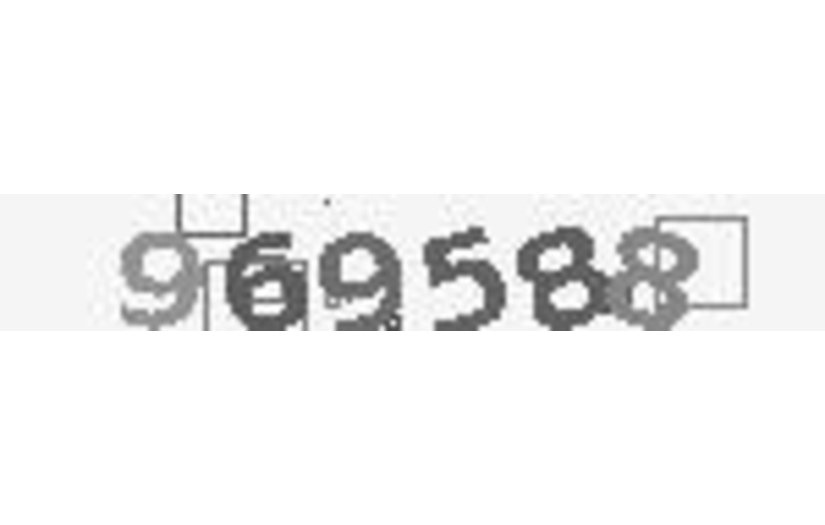
\includegraphics[width=0.2\textwidth,height=\textheight]{./pacote_files/figure-pdf/fig-exemplo-acesso-trf5-1.pdf}

}

\caption{\label{fig-exemplo-acesso-trf5}Exemplo de Captcha baixado
diretamente do TRF5.}

\end{figure}

Agora, aplica-se a função \texttt{captcha\_test\_trf5()} para verificar
se o rótulo está correto ou incorreto. A verificação é feita de forma
automática, diretamente da \emph{internet}, através do oráculo. A função
recebe dois parâmetros: \texttt{obj=} com as informações obtidas da
função de acesso; e \texttt{label=}, o rótulo obtido. A função retorna
\texttt{TRUE} se o rótulo está correto e \texttt{FALSE} caso contrário.

\begin{Shaded}
\begin{Highlighting}[]
\NormalTok{(acertou }\OtherTok{\textless{}{-}}\NormalTok{ captchaDownload}\SpecialCharTok{:::}\FunctionTok{captcha\_test\_trf5}\NormalTok{(acesso, lab))}
\end{Highlighting}
\end{Shaded}

\begin{verbatim}
[1] TRUE
\end{verbatim}

Cada Captcha possui uma função de acesso e uma função de teste. Na
prática, se uma pessoa desejar resolver um novo Captcha usando a técnica
do oráculo, são essas funções que ela precisar desenvolver. Todas as
outras operações podem ser generalizadas para diferentes casos de uso e
estão implementadas nos pacotes \texttt{\{captchaDownload\}} e
\texttt{\{captchaOracle\}}. Vale notar que a construção dessas funções
geralmente é necessária para a construção de \emph{web scrapers}, ou
seja, elas não criam dificuldades adicionais para pessoas interessadas
em resolver Captchas para acessar dados da \emph{internet}.

A função principal do pacote \texttt{\{captchaDownload\}} é a
\texttt{captcha\_oracle()}. A função é responsável por realizar a
anotação parcial automática dos Captchas utilizando um modelo inicial e
o oráculo. A função possui os seguintes parâmetros:

\begin{itemize}
\tightlist
\item
  \texttt{path=}: caminho em que os arquivos serão salvos.
\item
  \texttt{model=}: modelo para predizer o rótulo de uma imagem.
\item
  \texttt{max\_ntry=}: quantidade máxima de chutes até desistir.
\item
  \texttt{manual=}: caso o máximo de tentativas seja alcançado, abrir o
  \emph{prompt} para anotar manualmente? Por padrão, sim.
\item
  \texttt{captcha\_access=}: função que baixa um Captcha e retorna dados
  da sessão para validar o Captcha, como mostrada anteriormente.
\item
  \texttt{captcha\_test=}: função que testa se um Captcha está correto a
  partir de um rótulo específico, como mostrado anteriormente.
\end{itemize}

A função amarra todos os conceitos necessários para criar novas bases de
dados de forma automática. Primeiro, considera o caminho para salvar os
dados. Em seguida, considera o modelo e formas de lidar com o oráculo.
Por último, recebe as funções de acesso e de teste do Captcha. A função
escreve um arquivo de \emph{log} com os resultados dos testes. O arquivo
contém \texttt{max\_ntry} linhas, podendo ter uma linha adicional se
\texttt{manual=TRUE}, já que, se o modelo errar todas os chutes, a
anotação manual deve ser adicionada.

No exemplo do TRF5, a chamada da função \texttt{captcha\_oracle()} com
um chute ficaria da seguinte forma:

\begin{Shaded}
\begin{Highlighting}[]
\NormalTok{modelo\_trf5 }\OtherTok{\textless{}{-}} \FunctionTok{captcha\_load\_model}\NormalTok{(}\StringTok{"trf5"}\NormalTok{)}

\NormalTok{captchaDownload}\SpecialCharTok{::}\FunctionTok{captcha\_oracle}\NormalTok{(}
  \AttributeTok{path =} \StringTok{"assets/img/"}\NormalTok{,}
  \AttributeTok{model =}\NormalTok{ modelo\_trf5, }
  \AttributeTok{max\_ntry =} \DecValTok{1}\NormalTok{,}
  \AttributeTok{manual =} \ConstantTok{TRUE}\NormalTok{, }
  \AttributeTok{captcha\_access =}\NormalTok{ captchaDownload}\SpecialCharTok{:::}\NormalTok{captcha\_access\_trf5,}
  \AttributeTok{captcha\_test =}\NormalTok{ captchaDownload}\SpecialCharTok{:::}\NormalTok{captcha\_test\_trf5}
\NormalTok{)}
\end{Highlighting}
\end{Shaded}

\begin{verbatim}
✔ Acertou!!!
\end{verbatim}

No teste do exemplo, a função acertou, salvando o seguinte arquivo de
\emph{log}. Espaços foram adicionados para facilitar a visualização.

\begin{verbatim}
ntry, label , type, result
1,    569328, auto, TRUE
\end{verbatim}

Abaixo, foi colocado um modelo ruim para o TRT, para forçar o modelo a
errar todos os chutes. O resultado é o log abaixo

\begin{Shaded}
\begin{Highlighting}[]
\NormalTok{modelo }\OtherTok{\textless{}{-}} \FunctionTok{captcha\_load\_model}\NormalTok{(}\StringTok{"assets/modelo\_ruim.pt"}\NormalTok{)}

\NormalTok{captchaDownload}\SpecialCharTok{::}\FunctionTok{captcha\_oracle}\NormalTok{(}
  \AttributeTok{path =} \StringTok{"assets/img/"}\NormalTok{,}
  \AttributeTok{model =}\NormalTok{ modelo, }
  \AttributeTok{max\_ntry =} \DecValTok{10}\NormalTok{,}
  \AttributeTok{manual =} \ConstantTok{TRUE}\NormalTok{, }
  \AttributeTok{captcha\_access =}\NormalTok{ captchaDownload}\SpecialCharTok{:::}\NormalTok{captcha\_access\_trt,}
  \AttributeTok{captcha\_test =}\NormalTok{ captchaDownload}\SpecialCharTok{:::}\NormalTok{captcha\_test\_trt}
\NormalTok{)}
\end{Highlighting}
\end{Shaded}

\begin{verbatim}
ℹ Temos 10 candidatos...
ℹ Errou! O chute foi: v2su7w
ℹ Errou! O chute foi: t2su7w
ℹ Errou! O chute foi: v2su7y
ℹ Errou! O chute foi: t2su7y
ℹ Errou! O chute foi: y2su7w
ℹ Errou! O chute foi: v2su7h
ℹ Errou! O chute foi: t2su7h
ℹ Errou! O chute foi: y2su7y
ℹ Errou! O chute foi: v2wu7w
Label: v2xu7w
\end{verbatim}

No novo exemplo, a função errou todos os dez chutes, salvando o seguinte
arquivo de \emph{log}. Espaços foram adicionados para facilitar a
visualização. O último valor é um rótulo inserido manualmente.

\begin{verbatim}
ntry,  label,   type, result
   1, v2su7w,   auto,  FALSE
   2, t2su7w,   auto,  FALSE
   3, v2su7y,   auto,  FALSE
   4, t2su7y,   auto,  FALSE
   5, y2su7w,   auto,  FALSE
   6, v2su7h,   auto,  FALSE
   7, t2su7h,   auto,  FALSE
   8, y2su7y,   auto,  FALSE
   9, v2wu7w,   auto,  FALSE
  10, 92su7w,   auto,  FALSE
  NA, v2xu7w, manual,   TRUE
\end{verbatim}

Se o parâmetro \texttt{manual=FALSE} e o modelo não consegue acertar o
rótulo, a função também adiciona a mensagem:

\begin{verbatim}
✖ Errado depois de todas as tentativas...
\end{verbatim}

Em alguns casos, é possível que a função realize menos do que
\texttt{max\_ntry} chutes. Isso acontece quando a probabilidade do
melhor rótulo depois do chute errado é muito pequena, segundo o modelo.
Isso é feito pela função \texttt{captcha\_candidates()}, que considera
como padrão o corte de \texttt{0.01} de probabilidade. Ou seja, na
prática, a função testa no máximo os \texttt{max\_ntry} rótulos com
probabilidades maior que \texttt{0.01} segundo o modelo.

Em resumo, o pacote \texttt{\{captchaDownload\}} contém toda a parte de
\emph{web scraping} utilizada no desenvolvimento da tese.
Adicionalmente, o pacote contém funções para orquestrar o
\emph{download} automático de Captchas parcialmente rotulados, a partir
de um modelo inicial e um oráculo.

Os dados fornecidos pelo pacote ficam tanto na forma de imagens
rotuladas quanto na forma de arquivos de \emph{log}, disponibilizados em
arquivos \emph{CSV}. Para lidar com essa estrutura de dados, mais um
pacote foi desenvolvido: o \texttt{\{captchaOracle\}}, definido a
seguir.

\hypertarget{sec-pacote-oracle}{%
\section{Pacote captchaOracle}\label{sec-pacote-oracle}}

O pacote \texttt{\{captchaOracle\}}, assim como o
\texttt{\{captchaDownload\}}, foi desenvolvido para a construção da
tese. O pacote, portanto, não apresenta documentação extensiva e suas
funções podem não estar com a sintaxe final. Futuramente, o pacote
poderá funcionar como novo \emph{backend} para o pacote
\texttt{\{captcha\}}, aplicando o WAWL como uma alternativa no fluxo de
resolução de Captchas definido na Subseção \ref{sec-captcha-do-zero}.

O pacote possui quatro funções principais: a
\texttt{captcha\_dataset\_oracle()}, a \texttt{net\_captcha\_oracle()},
a \texttt{oracle\_loss()} e a \texttt{captcha\_accuracy\_oracle()}. Cada
função desempenha um papel similar a seus pares do pacote
\texttt{\{captcha\}}, mas conseguem lidar com a estrutura de dados
fornecida pelo oráculo.

A primeira função a ser utilizada é a
\texttt{captcha\_dataset\_oracle()}. Trata-se de uma função similar à
\texttt{captcha\_dataset()} do pacote \texttt{\{captcha\}}, mas com um
parâmetro adicional, \texttt{path\_logs=}, que recebe o caminho dos
arquivos de \emph{log}.

A estrutura de dados no caso do oráculo é mais complexa do que no caso
canônico. Na resposta, ao invés de guardar uma matriz \emph{one hot}
para cada Captcha, é armazenada uma lista com várias matrizes \emph{one
hot}, uma para cada tentativa do Captcha. Além disso, é armazenado um
vetor \texttt{z}, com zeros e uns, informando se algum rótulo está
correto ou se todos os rótulos estão incorretos. A variável \texttt{z} é
construída a partir dos nomes dos arquivos, que contém um \texttt{\_1}
caso o rótulo esteja correto e \texttt{\_0} caso contrário. Por último,
a imagem de entrada é armazenada da mesma forma que na função
\texttt{captcha\_dataset()}.

O módulo \texttt{net\_captcha\_oracle()} faz poucos ajustes à estrutura
inicial fornecida pelo módulo \texttt{net\_captcha()} do pacote
\texttt{\{captcha\}}. A única modificação da função é que ela recebe um
modelo inicial de entrada, transferindo os pesos ajustados do modelo ao
novo módulo. O módulo \texttt{net\_captcha\_oracle()}, inclusive,
poderia ser utilizado fora do contexto do WAWL, já que só utiliza os
dados de \emph{input}, que não são alterados.

A função \texttt{captcha\_accuracy\_oracle()} é utilizada para estimar a
acurácia do modelo. Para isso, a função precisa lidar com o fato de que
os dados de validação apresentam uma estrutura diferente dos dados de
treino, já que estão completamente anotados. No treino, a acurácia é
calculada considerando apenas os casos em que a resposta é conhecida. Na
validação, a acurácia é calculada considerando-se todas as observações.

Por último, a função \texttt{oracle\_loss()} é a que contém a proposta
de função de perda do método WAWL. Nos casos corretos, a função de perda
é obtida calculando-se uma entropia cruzada simples. Nos casos
incorretos, a perda é calculada pela estratégia \texttt{1-p}, ou seja,
considerando o complementar da probabilidade de observar os chutes que
foram apresentados segundo o modelo.

Em resumo, o pacote \texttt{\{captchaOracle\}} é o que contém os
principais avanços da tese do ponto de vista estatístico. Na prática, é
utilizado como \emph{backend} computacional para ajuste dos modelos que
utilizam o oráculo, dentro de um fluxo de trabalho igual ao que é
construído para ajuste dos modelos canônicos.

Os códigos para realizar as simulações do modelo foram adicionados na
pasta \texttt{data-raw} do pacote \texttt{\{captchaOracle\}}. Os códigos
foram organizados da seguinte forma:

\begin{itemize}
\tightlist
\item
  \texttt{passo\_01\_*.R}. Contêm os códigos utilizados para ajustar os
  modelos iniciais. Os códigos são organizados de forma a permitir que
  vários modelos sejam rodados em paralelo, aproveitando o máximo do
  poder computacional da máquina utilizada para realizar os ajustes.
\item
  \texttt{passo\_02\_*.R}. Contêm os códigos utilizados para construir
  as bases de treino e validação para o passo 03. Foi o passo mais
  demorado da simulação, já que envolveu acessar os sites dos tribunais
  pela \emph{internet} para obtenção dos Captchas anotados
  automaticamente. Para realizar a simulação, foram baixados mais de
  500.000 Captchas da \emph{internet}.
\item
  \texttt{passo\_03\_*.R}. Contêm os códigos utilizados para ajustar os
  modelos finais. Os códigos foram organizados de forma similar ao passo
  01, mas utilizando as funções desenvolvidas no pacote
  \texttt{\{captchaOracle\}} para considerar os dados fornecidos pelo
  oráculo.
\end{itemize}

Por fim, foi adicionado também um script \texttt{report.R}, que monta as
bases principais e os resumos dos modelos ajustados. As bases fornecidas
pelo último \emph{script} foram adicionadas ao repositório da tese.

% \input{conteudo/00-exemplo-introducao}
% \input{conteudo/01-exemplo-normas-ime}
% \input{conteudo/02-exemplo-usando-o-modelo}
% \input{conteudo/03-exemplo-latex}
% \input{conteudo/04-exemplo-tutorial}
% \input{conteudo/05-exemplo-exemplos}


%%%%%%%%%%%%%%%%%%%%%%%%%%%% APÊNDICES E ANEXOS %%%%%%%%%%%%%%%%%%%%%%%%%%%%%%%%

% Um apêndice é algum conteúdo adicional de sua autoria que faz parte e
% colabora com a ideia geral do texto mas que, por alguma razão, não precisa
% fazer parte da sequência do discurso; por exemplo, a demonstração de um
% teorema intermediário, as perguntas usadas em uma pesquisa qualitativa etc.
%
% Um anexo é um documento que não faz parte da tese (em geral, nem é de sua
% autoria) mas é relevante para o conteúdo; por exemplo, a especificação do
% padrão técnico ou a legislação que o trabalho discute, um artigo de jornal
% apresentando a percepção do público sobre o tema da tese etc.
%
% Os comandos appendix e annex reiniciam a numeração de capítulos e passam
% a numerá-los com letras. "annex" não faz parte de nenhuma classe padrão,
% foi criado para este modelo. Se o trabalho não tiver apêndices ou anexos,
% remova estas linhas.
%
% Diferentemente de \mainmatter, \backmatter etc., \appendix e \annex não
% forçam o início de uma nova página. Em geral isso não é importante, pois
% o comando seguinte costuma ser "\chapter", mas pode causar problemas com
% a formatação dos cabeçalhos. Assim, vamos forçar uma nova página antes
% de cada um deles.

%%%% Apêndices %%%%

\makeatletter
\if@openright\cleardoublepage\else\clearpage\fi
\makeatother

% \pagestyle{appendix}

% \appendix

% \addappheadtotoc acrescenta a palavra "Apêndice" ao sumário; se
% só há apêndices, sem anexos, provavelmente não é necessário.
% \addappheadtotoc

% \input{conteudo/apendice-exemplo-pseudocodigo}
% \par

%%%% Anexos %%%%

% \makeatletter
% \if@openright\cleardoublepage\else\clearpage\fi
% \makeatother

% \pagestyle{appendix} % repete o anterior, caso você não use apêndices

% \annex

% \addappheadtotoc acrescenta a palavra "Anexo" ao sumário; se
% só há anexos, sem apêndices, provavelmente não é necessário.
% \addappheadtotoc

% \input{conteudo/anexo-exemplo-faq}
% \par


%%%%%%%%%%%%%%% SEÇÕES FINAIS (BIBLIOGRAFIA E ÍNDICE REMISSIVO) %%%%%%%%%%%%%%%%

% O comando backmatter desabilita a numeração de capítulos.
\backmatter

\pagestyle{backmatter}

% Espaço adicional no sumário antes das referências / índice remissivo
\addtocontents{toc}{\vspace{2\baselineskip plus .5\baselineskip minus .5\baselineskip}}

% A bibliografia é obrigatória

\printbibliography[
  title=\refname\label{bibliografia}, % "Referências", recomendado pela ABNT
  %title=\bibname\label{bibliografia}, % "Bibliografia"
  heading=bibintoc, % Inclui a bibliografia no sumário
]

% \printindex % imprime o índice remissivo no documento (opcional)

\end{document}
